\providecommand{\classoptions}{keys}
\documentclass[noworkareas,deliverables,svgnames,\classoptions]{euproposal}       % for writing
%\documentclass[submit,noworkareas,deliverables]{euproposal}        % for submission
%\documentclass[submit,public,noworkareas,deliverables]{euproposal} % for public version

\usepackage[utf8]{inputenc}
%\usepackage{minitoc}

\usepackage{float}  % used to suppress floating of tables in Resources section.
\usetikzlibrary{calc,fit,positioning,shapes,arrows,snakes}

\addbibresource{../lib/kbibs/kwarcpubs.bib}
\addbibresource{../lib/kbibs/extpubs.bib}
\addbibresource{../lib/kbibs/kwarccrossrefs.bib}
\addbibresource{../lib/kbibs/extcrossrefs.bib}
\addbibresource{bibliography.bib}
% temporary fix due to http://tex.stackexchange.com/questions/311426/bibliography-error-use-of-blxbblverbaddi-doesnt-match-its-definition-ve
\makeatletter\def\blx@maxline{77}\makeatother

%%% institutions
\WAinstitution[id=PS,
        countryshort=FR,
        acronym=UPSud]
        {Universit\'e Paris-Sud}

\WAinstitution[id=LL,
        countryshort=FR,
        acronym=Logilab]
        {Logilab}

\WAinstitution[id=UV,
        countryshort=FR,
        acronym=UVSQ]
        {Universit\'e de Versailles Saint-Quentin}

\WAinstitution[id=UJF,
        countryshort=FR,
        acronym=UGA]
        {Universit\'e Grenoble Alpes}

\WAinstitution[id=UB,
        countryshort=FR,
        acronym=CNRS]
        {CNRS}

\WAinstitution[id=UO,
        countryshort=UK,
        acronym=UOXF]
        {University of Oxford}

\WAinstitution[id=USH,
        countryshort=UK,
        acronym=USFD]
        {University of Sheffield}

\WAinstitution[id=USO,
        countryshort=UK,
        acronym=SOUTHAMPTON]
        {University of Southampton}

\WAinstitution[id=SA,
        countryshort=UK,
        acronym=USTAN]
        {University of St Andrews}

\WAinstitution[id=UW,
        countryshort=UK,
        acronym=UWarwick]
        {University of Warwick}

\WAinstitution[id=JU,
        countryshort=DE,
        acronym=JacobsUni]
        {Jacobs University Bremen}

\WAinstitution[id=FAU,
        countryshort=DE,
        acronym=FAU]
        {Friedrich-Alexander Universit\"at Erlangen/N\"urnberg}

\WAinstitution[id=UK,
        countryshort=DE,
        acronym=UNIKL]
        {University of Kaiserslautern}

\WAinstitution[id=US,
        countryshort=PL,
        acronym=USlaski]
        {University of Silesia}

\WAinstitution[id=ZH,
        countryshort=CH,
        acronym=UZH]
        {Universit\"{a}t Z\"{u}rich}

\WAinstitution[id=SR,
        countryshort=NO,
        acronym=Simula]
        {Simula Research Laboratory}

\WAinstitution[id=UG,
	countryshort=BE,
	acronym=UGent]
	{Ghent University}

\WAinstitution[id=XFEL,
        countryshort=DE,
        acronym=XFEL]
        {European XFEL GmbH}

% \WAinstitution[id=UWS,
%         countryshort=US,
%         acronym=UWS]
%         {University of Washington at Seattle}

% \WAperson[id=miko, 
%            personaltitle=Prof. Dr.,
%            birthdate=13. September 1964,
%            academictitle=Professor of Computer Science,
%            affiliation=jacu,
%            department=case,
%            privaddress=None of your business,
%            privtel=that neither,
%            email=m.kohlhase@jacobs-university.de,
%            workaddress={Campus Ring 1, 28757 Bremen},
%            worktel=+49 421 200 3140,
%            worktelfax=+49 421 200 3140/493140,
%            workfax=+49 421 200 493140]
%            {Michael Kohlhase}

\WAperson[id=thiery,
           personaltitle=Prof. ,
           birthdate=28 Mai 1973,
           academictitle=Professor of Computer Science,
           affiliation=PS,
           department=Laboratoire de Recherche en Informatique,
           privaddress=None of your business,
           privtel=that neither,
           email=Nicolas.Thiery@u-psud.fr,
           workaddress={Campus Ring 1, 28757 Bremen},
           %worktel=+33 6 77 90 32 79,
           worktelfax=+33 6 77 90 32 79,
           %workfax=N/A
           ]
           {Nicolas M. Thiéry}

%%% Local Variables: 
%%% mode: latex
%%% TeX-master: "proposal"
%%% End: 

% LocalWords:  WAperson miko personaltitle academictitle privaddress privtel Sud
% LocalWords:  workaddress worktel workfax gc worktelfax pcg pcsa WAinstitution
% LocalWords:  shortname partof streetaddress townzip countryshort efo 3kd89
% LocalWords:  jacobs-logo.png Seefahrtstrasse Kruislann Montparnasse Universit
% LocalWords:  baz Westerfield
 % Some sections of the included files depend on this.
\usepackage{lscape} % for landscape
\usepackage{comments}
% %\usepackage[final]{comments}
\usepackage{verbatim}
\usepackage{listings}
\usepackage{supertabular,array}
\makeatletter
\newcommand\arraybslash{\let\\\@arraycr}
\makeatother
% \setlength\tabcolsep{1mm}
% \renewcommand\arraystretch{1.3}
%% Related Projects
\newcommand{\scienceproject}{\mbox{\textsc{SCIEnce}}\xspace}
\newcommand{\OOMMF}{OOMMF\xspace}
\newcommand{\OOMMFNB}{OOMMF-NB\xspace}
\newcommand{\ODK}{OpenDreamKit\xspace}
\newcommand{\VRE}{VRE\xspace}
\newcommand{\VREs}{VRE\xspace}
\newcommand{\software}[1]{\textsc{#1}\xspace}
\newcommand{\GAP}{\software{GAP}}
\newcommand{\HPCGAP}{\software{HPC-GAP}}
\newcommand{\libGAP}{\software{libGAP}}
\newcommand{\Singular}{\software{Singular}}
\newcommand{\Sage}{\software{Sage}}
\newcommand{\SageCombinat}{\software{Sage-Combinat}}
\newcommand{\MuPADCombinat}{\software{MuPAD-Combinat}}
\newcommand{\Sphinx}{\software{Sphinx}}
\newcommand{\SCSCP}{\software{SCSCP}}
\newcommand{\JavaScript}{\software{JavaScript}}
\newcommand{\Python}{\software{Python}}
\newcommand{\IPython}{\software{IPython}}
\newcommand{\Jupyter}{\software{Jupyter}}
\newcommand{\JupyterHub}{\software{JupyterHub}}
\newcommand{\Cython}{\software{Cython}}
\newcommand{\Pythran}{\software{Pythran}}
\newcommand{\Numpy}{\software{Numpy}}
\newcommand{\Pari}{\software{PARI}}
\newcommand{\PariGP}{\software{PARI/GP}}
\newcommand{\libpari}{\software{libpari}}
\newcommand{\GP}{\software{GP}}
\newcommand{\GPtoC}{\software{GP2C}}
\newcommand{\Linbox}{\software{LinBox}}
\newcommand{\LMFDB}{\software{LMFDB}}
\newcommand{\OpenEdX}{\software{OpenEdX}}
\newcommand{\Linux}{\software{Linux}}
\newcommand{\LATEX}{\software{\LaTeX}}
\newcommand{\SMC}{\software{SageMathCloud}}
\newcommand{\Simulagora}{\software{Simulagora}}
\newcommand{\KANT}{\software{KANT}}
\newcommand{\Magma}{\software{Magma}}
\newcommand{\Mathematica}{\software{Mathematica}}
\newcommand{\Maple}{\software{Maple}}
\newcommand{\Matlab}{\software{Matlab}}
\newcommand{\MuPAD}{\software{MuPAD}}
\newcommand{\MPIR}{\software{MPIR}}
\newcommand{\Arxiv}{\software{arXiv}}
\newcommand{\Givaro}{\software{Givaro}}
\newcommand{\fflas}{\software{fflas}}
\newcommand{\MathHub}{\software{MathHub}}
\newcommand{\FindStat}{\software{FindStat}}
\newcommand{\GitHub}{\software{GitHub}}
\newcommand{\git}{\software{git}}
\newcommand\DKS{\ensuremath{\mathcal{DKS}}\xspace}
\newcommand{\FLINT}{\software{FLINT}}

%%% Local Variables: 
%%% mode: latex
%%% TeX-master: "proposal"
%%% End: 

\usepackage{framed}

\begin{document}
\begin{proposal}[
  % These PM numbers (person months) are for the coordinator to help planning
  % Participants should not change these, but add PM numbers in the CVS in
  % the site descriptions at CVs/*.tex
  % TODO: Nicolas needs to update these numbers from the (requested ones)
  site=PS, %paris sud
  site=UB,   % CNRS (Bordeaux)
  site=JU,  % Jacobs University Bremen
  site=UJF, % Univ Josef Fourier Grenoble
  site=UK, % Kaiserslautern
  site=UO, % Oxford
  site=US, % Silesia
  site=USH, % Sheffield
  site=USO, % Southhampton
  site=SA, % St Andrews
  site=UV, % Versailles
  site=UW, % Warwick
  site=ZH, % Z"urich
  site=LL, % logilab
  site=SR, % Simula
  site=UG, % Gent
  site=FAU, % FAU Erlangen/Nuremberg
  site=XFEL, % European XFEL GmbH
  site=LEEDS, % Leeds
  botupPM, % we want to work via bottom up PM distribution,
  % alternative: (can be combined)
  % topdownPM, % the coordinator distributes PM as follows:
  % PSRM=48, %paris sud
  % LLRM=48, % logilab
  % UVRM=48, % Versailles
  % UJFRM=48, % Fourier
  % UBRM=48,   % CNRS (Bordeaux)
  % UORM=48, % Oxford
  % USHRM=48, % Sheffield
  % USORM=48, % Southhampton
  % SARM=48, % St Andrews
  % UWRM=48, % Warwick
  % JURM=48,  % Jacobs
  % UKRM=48, % Kaiserslautern
  % USRM=48, % Silesia
  % ZHRM=48, % Z"urich
  % SRRM=48, % Simula
    coordinator=thiery,
  coordinatorsite=PS,
  acronym={OpenDreamKit},
  acrolong={OpenDreamKit},
  proposalnumber={676541},
  title=Open Digital Research Environment Toolkit\\ for the Advancement of Mathematics,
  callname=Topic: e-Infrastructures for Virtual Research Environments (VRE),
  callid=EINFRA-9-2015,
  % TODO: consistency with provided template
  % CALL: H2020-EINFRA-2015-1
  % TOPIC: e-Infrastructures for Virtual Research Environments (VRE)
  % Instrument: e-Infrastructures
  keywords={pure mathematics, computer algebra, simulation,
    visualisation, component architecture, databases, 
reproducibility, Sage, IPython, Jupyter, LMFDB, MathHub},
  % computational mathematics,
  % GAP, Linbox, PARI, Sage, Singular, IPython, Jupyter, SageMathCloud, LMFDB, MathHub
  % Virtual research environments, MPIR, /GP
  % open source, free software, number theory, abstract algebra, notebooks
  instrument= Call: H2020-EINFRA-2015-1, %Call: H2020-EINFRA-2015-1, 3 Topic 9-2015
  challengeid = TODO,
  %challenge = {N/A},
  %objectiveid={N/A},
  %objective = TODO,
  %outcomeid = N/A,
  %outcome = N/A,
  coordinator=thiery,
  months=48,
  compactht]
\newcommand{\TheProject}{\pn}% \pn is defined automatically
\section*{History of changes}

\subsection*{Grant agreement number 676541, June 2015}
\thispagestyle{empty}

\begin{enumerate}
\item Updated participant acronyms for consistency with the EU portal.

\item Resources for UPSud: reinstated PhD position that was planned in
  the budget but went missing in the proposal document: +36PM for UPSud.
\item Reinstated related task T6.5 ``Knowledge-based code infrastructure''.
  +33PM for WP6
\item Minor update to the involvement for Pons, Hivert, Lelièvre at
  UPSud for consistency with the submitted budget (-1PM each).
\item Minor update to the involvement for Gouarin at CNRS to make up
  for a higher salary than expected (-1PM); adapted accordingly WP2
  (-1PM).
\item Where relevant: updated PM information according to the above.

\item WP2: Added mention of our participation to the European
  E-Infrastructure concertation activities.

\item Updated resources to be committed: audit costs should be in the
  direct costs, not subcontracting.

\item Updated the risk table to address the reviewers comments.

\item As suggested by the project officer, reduction of the number of
  deliverables (typically by merging together intermediate
  check-points into the corresponding final deliverable):
  \begin{itemize}
  \item Suppressed irrelevant D1.1. (Consortium agreement).
  \item Removed accidently duplicated deliverables:
    \begin{itemize}
    \item D2.10 Course material on using OpenDreamKit in data science;
    \item D2.12, D2.13 indexing service;
    \item D2.20 Demonstrator: Interactive lecture notes and marking
      systems based on OpenDreamKit.
    \end{itemize}
  \item Merged together D1.5 and D1.8 (Data Management Plan V2,V3)
  \item Merged D2.2, D2.7, D2.14, D2.19, D2.25, and D2.26 (community
    building reports: impact of development and training workshops)
    into a single yearly report.
  \item Merged together D2.3, D2.15, D2.23, and D2.24 (Demonstrators:
    Problems in Physics with Sage v1,2 , Computational Mathematics for
    Engineering).
  \item Merged together D2.8 (Community-curated indexing tool (open
    source)) and D2.9 (Community-curated indexing service for
    OpenDreamKit).
  \item Merged D2.16 (Micromagnetic VRE code and documents source
    online), D3.4 (Python interface to OOMMF completed), D4.8
    (Micromagnetic VRE software completed), D4.11 (Micromagnetic VRE
    tutorial and documentation notebooks), and D4.14 (Demonstrator
    online portal available) into a single deliverable D2.13
    (Micromagnetic VRE completed and online).
  \item Merged D3.1 and D3.9 (one-click install Sage distribution for
    Windows with Cygwin 32bit/64bit).
  \item Merged D5.1 (Facility to compile \Pythran compliant user
    kernels and sage code) and D5.3 (Improve \Pythran runtime support
    to automatically take advantage of multi-cores and SIMD
    instruction units and use it in CYTHON); also switched lead info
    for D5.3 and D5.5 (Improve PYTHRAN typing to improve error
    information).
  \item Merged D5.9 (Report on development of designs for the GAP
    developments – parallel library, interacts to standard
    infrastructure and CYTHON-like extensions) and D5.15
    (Implementations of the GAP developments, ready for release) into
    D5.18 (Final report and evaluation of the GAP developments).
  \item Merged D6.1 (DKS base survey and Requirements Workshop Report)
    and D6.3 (initial DKS base Design).
  \item Merged D6.4 (Design of Triform (DKS) Theories
    (Specification/RNC Schema/Examples)) and D6.5 (Implementation of
    Triform Theories in the MMT API).
  \item Merged D6.6 (LMFDB deep modelling: Fragment Identification and
    Initial Model Design), D6.7 (Heuristic Parser for the OEIS Import,
    Cross Validation of DKS-Model), D6.8 (Conversion of existing and
    new Databases to unified interoperable System).
  \item Merged D6.10 (Full-text search (Formulae + Keywords) over
    Notebooks) and D6.12 (Formula search in CAS programs and Software
    Modules).
  \item Merged D7.1, D7.4, D7.7 (Reports on relevant research in
    sociology of mathematics and lessons for design of OpenDreamKit
    VRE, parts I, II, III).
  \end{itemize}
\end{enumerate}
\clearpage
\thispagestyle{empty}
\subsection*{1st amendment of the Grant Agreement, June 2016}

\begin{enumerate}
\item Addition of Ghent University (UGent) to the list of beneficiaries
\item Change of lead beneficiary from UPSud to UGent for D4.13
\item Addition of UGent the list of partners concerned by tasks: T1.1, T1.2, T1.3, T2.3, T3.1, T3.2, T3.3, T3.6, T3.7, T4.1, T4.4, T4.5, T4.12
\item Change of participation to WP1: 26.5 PM for UPSud and 1.5 PM fpr UGent
\item Change of participation to WP2: 9 PM for UPSud and 1 PM for UGent
\item Change of participation to WP3: 50 PM for UPSud and 14 PM for UGent
\item Change of participation to WP4: 12 PM for UPSud and 14 PM for UGent
\item Allocation of resources to UGent following their addition
\item Equivalent reduction of UPSud's resources following the addition of UGent
\item Reshuffling of resources allocated to JacobsUni following the
  organisation of an extra workshop (no change to their total budget)
\item Some deliverables are postponed, mostly due to difficulties in the recruitment process: D2.13, D3.2, D4.2, D5.2
\item Some tasks are postponed, mostly due to difficulties in the recruitment process: T2.7, T2.8, T2.9, T3.8, T4.11, T4.13, T4.14, T7.4
\item Stripped erroneously included pages about WP7 (page numbered 54
  and 55 between 29 and 31); inserted missing page 30 about
  milestones.
\item Fixed minor typos in the texts.
\end{enumerate}
\clearpage
\thispagestyle{empty}
\subsection*{2nd amendment of the Grant Agreement, March 2017}
\ednote{insert month when ready}
\begin{enumerate}
\item Accomodate the move of the KWARC Group (Prof Michael Kohlhase) from \site{JU} to
  \site{FAU}.
\begin{enumerate}
\item Addition of Friedrich Alexander University Erlangen/Nuremberg (\site{FAU}) to the
  list of beneficiaries.
\item \WPref{management}: moved 1 PM from \site{JU} to \site{FAU}.
\item \WPref{dksbases}: Made \site{FAU} lead of \WPref{dksbases} (even though JU had been
  for the initial phase), moved 34 PM and the lead of all deliverables after month 15 from
  \site{JU} to \site{FAU}.
\item \WPref{UI}: moved 8 PM and the lead of all deliverables after month 15 from
  \site{JU} to \site{FAU}.
\item Resources (Section~\ref{sec:resources}): moved the respective resources from
  \site{JU} to \site{FAU}.
\end{enumerate}
\item \WPref{dksbases}: adapted the titles of \delivref{dksbases}{psfoundation},
  \delivref{dksbases}{pssem}, and \delivref{dksbases}{lfmverif} to respect the change in
  priority on system interoperability and distributed computing in the
  ``Math-in-the-Middle'' Paradigm over algorithm verification.
\item Changed the lead of \delivref{component-architecture}{semantic-interface-sage-gap}
  from \site{UO} to \site{PS}, and the lead of \delivref{dksbases}{lfmverif} from \site{ZH} to \site{FAU}
\item Changed the lead of \site{USH} from Neil Lawrence to Michael Croucher, and the breakdown
of Person-Month to be used by this site (within the frame of the 360,00.00€ of their Personnel Costs)
\item Typo fix: \delivref{UI}{ipython-kernels} was meant to be due M24, not M14.
\item Changed the lead PI of \site{UO} from Ursula Martin to Dmitrii Pasechnik
\item Changed the lead PI of \site{SR} from Hans-Peter Langtangen to Martin A. Sandves
\item \site{UJF} changed name from Universite Joseph Fourier to Universite Grenoble Alpes
\item \site{PS} changed its PhD position of 36 PM into a Postdoc position of 24 PM
  Reduced accordingly \site{PS}'s involvement in PM's in \WPref{dksbases}.
\item Consistency fix for \site{PS}: adjusted involvement in \WPref{component-architecture} from 50~PM to 46~PM and reduced accordingly the PM's
  requested in \site{PS}'s description for research engineers: upon
  the transfer to UGent, those figures had been incorrectly updated in
  the 1st amendment.
\item Accommodate the move of Hans Fangohr from \site{USO} to
  \site{XFEL}.
\begin{enumerate}
\item Addition of European XFEL GmbH/Schenefeld (\site{XFEL}) to the
  list of beneficiaries.
\item \WPref{management}: moved 1 PM from \site{USO} to \site{XFEL}.
\item \WPref{dissem}:  Moved 15 PM and the lead of all tasks to be
  completed after month 24 and the deliverable \delivref{dissem}{oommfnb-vre-deliver} from
  \site{USO} to \site{XFEL}.
\item \WPref{UI}: moved 5 PM from \site{USO} to \site{XFEL}.
\item \WPref{social-aspects}: moved deliverable D7.8 and 6 PM from
  \site{USO} to \site{XFEL}. % D7.8 is explicitly written here because
                             % it is removed in the next proposal
                             % change and we cannot refer to it
                             % anymore (MB).

\item Resources (Section~\ref{sec:resources}): moved the respective resources from
  \site{USO} to \site{XFEL}.

\item Removed 4,000 EUR for open access publication charges from
  Southampton (were by mistake omitted in submission and are thus not available).
\end{enumerate}


\item  Clarification of the CNRS site situation
\begin{enumerate}
\item Added S\'ebastien Labb\'e as a member of CNRS and removed 18 PM for
  the recruited engineer.
\item Clarification of PM repartition between CNRS and its third
  party University of Bordeaux
Removed 28,198 EUR from "Other goods and services" from
  CNRS in order to take into account modifications in Person-Months
  involved in the project. This will have no impact on the deliverables
  in which CNRS is involved.
\end{enumerate}

\item Postponment of deliverables within the first Reporting Period
\begin{enumerate}
\item \delivref{UI}{pari-python-lib1} from M6 to M18
\item \delivref{UI}{mathhub-editing} from M12 to M18
\item \delivref{hpc}{pythran-typing} from M12 to M18
\end{enumerate}

\item Some deliverables names in \WPref{hpc} were modified
\begin{enumerate}
\item \delivref{hpc}{MPIRsuperoptimiser} from "Extend the existingassembly superoptimiser
for AVX and upcoming Intel processor extensions for the MPIR library" to "Write an assembly
superoptimiser supporting AVX and upcoming Intel processor extensions for the MPIR library
and optimise MPIR for modern processors"
\item \delivref{hpc}{QS-linalg} from"Parallelise the relation sieving component of the
Quadratic Sieve and implement a parallel version of Block-Wiederman linear algebra over GF2
and the triple large prime variant" to "Parallelise the relation sieving component of the
Quadratic Sieve and implement a parallel version of Block-Wiederman linear algebra over GF2
and implement large prime variants"
\item \delivref{hpc}{FFT} from "Take advantage of multiple cores in the matrix Fourier Algorithm
component of the FFT for integer and polynomial arithmetic,and include assembly primitives for
SIMD processor instructions (AVX, Knight's Bridge, etc.), especially in the FFT butterflies" to
"Take advantage of multiple cores in the matrix Fourier Algorithm component of the FFT for
integer and polynomial arithmetic,and include assembly primitives for SIMD processor
instructions (e.g. AVX, etc.), especially in the FFT butterflies"
\end{enumerate}

\end{enumerate}

\clearpage
\thispagestyle{empty}
\subsection*{Work Plan revisions, Fall 2017}
\ednote{insert month when ready}

Following feedback from project officer and reviewers at the 18 month
project review, we are proposing the following revisions:
\begin{enumerate}
\item Reduction of number of deliverables:
  \begin{itemize}
  \item Merged \delivref{dissem}{workshops-2} into \delivref{dissem}{workshops-3}.
  \item Merged \delivref{dissem}{ibook2} into \delivref{dissem}{ibook1}.
  \item Merged together \delivref{dissem}{datascience-course},
    \delivref{dissem}{lecture-notes} and \delivref{dissem}{notebook-repo} into \delivref{dissem}{IntroODK}

  \item Merged \delivref{component-architecture}{sage-repository} into \delivref{component-architecture}{sage-distribution}.

  \item Merged \delivref{UI}{cfd-vis} into \delivref{UI}{vis3d}, to be delivered in M36.

  \item Merged \delivref{hpc}{cython-pythran-cilk} into \delivref{hpc}{sage-HPCcombi}.
  \item Merged \delivref{hpc}{LinBox-DSL} into \delivref{hpc}{LinBox-distributed}.
  \item Merged \delivref{hpc}{pari-hpc1} into \delivref{hpc}{pari-hpc2}.

  \item Merged \delivref{dksbases}{conv} into \delivref{dksbases}{psfoundation}.
  \item Merged \delivref{dksbases}{lfmint} into \delivref{dksbases}{psfoundation} and
    \delivref{dksbases}{lfmverif}.
  \item Merged
    \delivref{component-architecture}{semantic-interface-sage-gap} and
    \delivref{dksbases}{pssem} into \delivref{dksbases}{lfmverif}.
  \item Merged \delivref{dksbases}{notebooksearch} into \delivref{dksbases}{nbad-search}.

  \item Merged \delivref{social-aspects}{oommf-nb-evaluation} into
    \delivref{dissem}{oommfnb-vre-deliver}.%, lead by \site{XFEL}.
  \end{itemize}

\item Integration of WP7 activities into other WPs:
  \begin{itemize}
  \item Integrated T7.4 in
    \taskref{dissem}{dissemination-of-oommf-nb-workshops}, lead by
    \site{XFEL}. Merged task is now
    \taskref{dissem}{dissemination-of-oommf-nb-workshops}.
  \item Canceled \taskref{social-aspects}{social-input} and associated deliverable \delivref{social-aspects}{social-report-three}, and moved PM to WP3.
  \item Canceled \taskref{social-aspects}{social-output} and associated deliverables \delivref{social-aspects}{jupyter-comment} , \delivref{social-aspects}{social-poster} and \delivref{social-aspects}{social-publishing-report} and moved PM to \taskref{dissem}{project-intro}.
  \item Canceled \taskref{social-aspects}{isocial-decisionmaking}, cancelled deliverables \delivref{social-aspects}{social-tracaddon} and \delivref{social-aspects}{social-gametheoretic}, and moved PM to WP3 and WP5.
  \end{itemize}
\item Work package specific milestones:
  \begin{itemize}
  \item Introduced one milestone at month 42 for
    \WPref{component-architecture}, two milestones at months 36 and 48
    for \WPref{UI}, one milestone at month 36 for \WPref{hpc} and two
    milestones at month 36 and 42 for \WPref{dksbases}.
  \item Removed redundant general milestone at month 36.
  \end{itemize}
\item New Key Performance Indicators introduced to better monitor the progress impact and results
  \begin{itemize}
  \item Four Indicators linked to the four project aims
  \item Focus on success stories and qualitative indicators in general
  \item Reusable, meaningful and realistic quantitative indicators decided by the steering committee
 
\item Miscellaneous
  \begin{itemize}
  \item Canceled \delivref{component-architecture}{personal-smc} as
    not relevant anymore: work has been done by the community. The
    corresponding workload has been reallocated, mostly to
    WorkPackage~\WPref{dissem}.
  \item \delivref{UI}{jupyter-import} moved from M24 to M36 to incorporate results
    from workshop on live structured documents.
  \item \taskref{UI}{notebook-collab} expanded from M1-M24 to M1-M48 (the full duration of the grant)
    to reflect the ongoing nature of the work. Activity, total work,
    and deliverables are unchanged.
  \item typo fix in deliverable title for \delivref{management}{ipr2}
    (reports for year 2 and 3, not just year 2).
  \item Modification of lead for WP6: from Jacobsuni to FAU
  \item Remove the HPC conference in Bordeaux in favor of more dissemination schools and workshops (no modification of resources)
  \item Termination of Jacobsuni on 31/12/2017: all relevant staff for the project was moved to FAU and UNiversité Paris-Sud
  \item Termination of UZH on 31/12/2017: all activity planned for the partner has been accomplished and resources were spent
  \end{itemize}
\end{enumerate}


\clearpage
\setcounter{page}{1}

%%% Local Variables:
%%% mode: latex
%%% TeX-master: "grantagreement"
%%% End:

\ifgrantagreement
\else
\clearpage
  Work Package WP6 develops a novel, foundational, knowledge-based framework for
  interfacing existing open source mathematical software systems and knowledge bases into
  a mathematical VRE, where systems can delegate functionalities among each other
  seamlessly without losing semantics.

  The overall Math-in-the-Middle (MitM) Framework developed in WP6 over the last three
  years is described in D6.5; this Report complements it by describing the curated
  contents Math-in-the-Middle (MitM) Ontology which serves as a reference and pivotal
  point for translations between the various input languages of mathematical software
  systems and knowledge bases.

  In a nutshell, the MitM Ontology describes the mathematical objects, concepts, and their
  relations in a general, system-agnostic way in an OMDoc/MMT theory graph while the
  mathematical systems export API theories that describe the system interface language in
  terms of types, classes, constructors, and functions -- again in OMDoc/MMT. These two
  levels of descriptions are linked by OMDoc/MMT alignments that allow the translation of
  expressions between systems.

%%% Local Variables:
%%% mode: visual-line
%%% fill-column: 5000
%%% mode: latex 
%%% TeX-master: "report"
%%% End:

\fi
\ifsubmit\else\setcounter{tocdepth}{4}\fi
\tableofcontents

\TOWRITE{MK}{Larger table of participants}
\TOWRITE{MK}{Abstract in the first page?}
\TOWRITE{MK}{Centering}

\begin{draft}
\section*{Outline of Project (for Proposers)}

\TODO{This is the place for various READMEs not included in the final submission}

\subsection*{Vision}

An internal attempt at specifying our vision through short
(unsubstantiated) answers.

\begin{verbatim}
> 1) Who are we?

Lead or core developers of some of the major open source components
for pure mathematics and applications:

- Computational components: GAP, Linbox, MPIR, Pari, Sage, Singular
- Databases: LMFDB (findstat as well)
- Knowledge management: MathHub

Together with, in a larger scientific domain, lead developers for:

- Collaborative user interfaces (IPython, SageMathCloud)
- Database and Scientific Computing for the industry (Logilab)
- Numerical code optimization/parallelisation (Pythran)

> 2) What is our goal?

Building blocks with a sustainable development model that can be
seamlessly combined together to build versatile high performance
VRE's, each tailored to a specific need in pure mathematics and
application.

> 2.5) What is our strategy?

Maximize sustainability and impact by reusing and improving existing
building blocks, and reaching toward larger communities whenever possible.
E.g. factoring out our common user interface needs at the level
of IPython/Jupyter will save us time (sustainability), and impact
the larger scientific computing community.
The improvements to the building blocks will impact all their users,
whether they use the VRE or not.

> 3) From where do we start?

- Building blocks with a sustainable development model
- Proof-of-concept prototypes of VRE (SMC, Simulagora)
- Experience on combining together some of the building blocks

> 4) How do we connect or differ from other projects?

The other projects focus on either one or a few of the building
blocks, or on a specific VRE.

We articulate our work with each of them.

> 5) Why are we excellent?

The consortium puts together recognized experts in all
areas and most building blocks that are relevant to the goal. There is
simultaneously a variety of point of views and a record of past
experiences collaborating together at smaller scale
(e.g. GAP-Singular). The approach is bottom up.  Most joint tasks
consist in bringing together people with a common need. There is
experience in community building.  Most participants are
simultaneously users and developers of their tools.

All of this makes me confident that we will indeed be able to
productively collaborate. And do stuff that is first class and useful.

On Sat, Dec 13, 2014 at 11:18:10PM +0100, Wolfram Decker wrote:
> 0) What precisely is our starting point and why are we the right people to
> achieve what we promise to do? Are we leaders in the area touched
> by the proposal? How do we connect? Is there some past
> collaborative success?
> 1) You still do not say what we actually will provide. What precisely will
> the VRE offer to its users?

I more or less answered those points above. Let me know if I should
elaborate.

> Who will be its users? Will those already familiar with the involved
> CAS use it? Will it make the CAS more attractive for a much larger
> community?

One objective is definitely to make CAS and others more attractive by
lowering a lot the entry barrier to access the soft (and db, ...). A
typical situation that most of us ran into is, when collaborating with
other less tech-savvy mathematicians, to have trouble sharing code,
data, and in-the-writing papers with them. SMC was launched with this
idea in mind, and the success proves the concept.

At the same time, the improvements in the building blocks will also
impact CAS users that are happy with their current user interface /
work-flow.

Improvements to IPython will impact a much larger community.

> 2) You motivate what we wish to do by the success of SageMathCloud.
> But why do we than need another VRE? How do we differ from
> SageMathCloud?

There is no one-size-fits-all VRE. One might want to run a VRE on
one's own computer resources for a variety of reason (speed of access,
specific resources, privacy, independence, ...). One might want a
different combination of software (e.g. a lightweight VRE with only
Singular).  One might want to focus on data with LMFDB-style database
searches, or on interactive computing, or on document writing, or some
combination thereof.

> Do we have a chance to compete? Or will we rather join forces? In
> which way?

We join forces (the plan is to have William/UW in the consortium, as
non funded participant). SMC focuses on one specific cloud based
VRE. We focus on the building blocks and the glue. Both project are
mutually beneficial. See the language p. 14 of the proposal.

> 3) You motivate what we wish to do by the success of LMFDB. But what
> are our connections to this database? Will we enhance it? Will we connect
> it to other stuff we do? Will we create other databases?

LMFDB is a prototype of large scale database. We want to make it
easier for other groups of mathematicians to set up similar databases
in their area. Reciprocally, like SMC, the LMFDB with benefit back
from the improved building blocks.

> 4) Why is Europe in the lead if there is already SageMathCloud?
> Where precisely is Europe in the lead?

Europe is the lead in many of the building blocks.
\end{verbatim}

% \subsection*{Mission statement for the grant}

% Our mission is to promote the next generation of community-developed
% open source software, databases, and services adapted to the needs of
% collaborative research in pure mathematics and applications.

% Our research will cover a wide variety of aspects, ranging from
% software development models, user interfaces \TODO{virtual
%   environments?}, deployment frameworks and novel collaborative tools,
% component architecture, design, and standardization of software
% \TODO{system?} and databases, to links to publication, data archival
% and reproducibility of experiments, development models and tools, and
% social aspects.

% It will consolidate Europe's leading position in computational
% mathematics and build on the remarkable success of the ecosystem of
% projects GAP, Python/Sage, Pari, Singular, LMFDB.

\subsection*{Description of the call}

\verbatiminput{call_description}

% \TODO{What do we mean by ``new generation''}.

\renewcommand{\thepage}{\arabic{page}}
\setcounter{page}{1}
\black
\cleardoublepage
\end{draft}

%%% Local Variables: 
%%% mode: latex
%%% TeX-master: "proposal"
%%% End: 

%  LocalWords:  verbatiminput renewcommand thepage setcounter cleardoublepage


% ---------------------------------------------------------------------------
%  Section 1: Excellence
% ---------------------------------------------------------------------------

\section{Excellence}
\TOWRITE{ALL}{Proofread 1. Excellence introduction pass 2}
% Some guiding questions of Wolfram:

% Agreed, but why is such a thing needed? "I have worked with CAS for
% years and I am fine with what is there". "I still can think with my
% own head and do not need a CAS". "I do not understand what a MathVre
% is".

% The art here is to explain in, say, at most 10-15 lines, why the
% design of CAS is a success story for math, what a MathVRE provides
% in addition and why we need it, and why we are the right people to
% create it. Again, we might even run into referees whom we first have
% to convince that CAS is a good thing to have!

\COMMENT{For good or bad, the ``pure math'' aspect does not appear in
  this introduction.}

\TOWRITE{All}{Try to include the following suggestions by Wolfram:
  \begin{compactitem}
  \item The mathematics involved has originally not been developed for
    the application (as for the Radon transform). It was already
    there, when needed.
  \item In a ever faster changing world, we need a reasonably ample
    mathematical algorithmic tool kit to choose from, when the need
    arises.
  \item At the beginning, applications have been dominated by inexact
    but fast numerical methods.  With more powerful computers
    available, exact computer algebra methods have become more and
    more crucial (examples such as cell phones, internet security.)
    Will now enter all application areas.
 \item  The things we provide are indispensable for the quick reactions needed
   and for allowing the potential applicants use the systems we develop
   (so far only used by specialists) Mention the success of mathlab as an
    important example on the numerical side.
  \end{compactitem}
}

% maths at the core of technology and innovation
\TOWRITE{All}{Improve the examples? Something from health care depending on
  pure maths?}

Improvements of the economy, ecology, health care, security and
society overall are driven by innovation. Key tools
for innovation are mathematical knowledge and
algorithms. Our global positioning system (GPS)
needs relativistic mathematics, our mobile phones are allocated frequencies through
combinatorial optimisation, the combinatorics of our genome yields clues to curing rare diseases, 
the privacy of our communications depends on cryptographic protocols steeped in number theory,  
and our national security is reliant on the mathematical analysis of increasingly complex networks. Engineering, Science and Business
innovations that enrich society and mankind are made possible through
mathematical foundations which are often developed long before their potential
applications.
%
% recent developments
Reciprocally, modern mathematical research is increasingly accelerated by and
enabled through collaborative tools, computational environments and
online databases. These digital tools have the potential to
revolutionise the way research is conducted.

% what is this proposal about - aim
In this project, we will provide mathematicians and scientists with a
generic unified toolkit, the Open Digital Research Environment Toolkit
for the Advancement of Mathematics (\TheProject), that allows
building of specific \emph{Virtual Research Environments} (VREs) for
particular tasks and communities.
%and (ii) more effective communication of research.


% How will we achieve this?
We will achieve this by focusing on a \emph{toolkit of software
  components} from which \emph{tailored VREs can be assembled
  flexibly} to cater for the diversity and evolution of needs in
mathematics, science and engineering.  We are at a critical point providing
an opportunity to do so: collaborative tools for code sharing (e.g.
\texttt{github}) now allow us to bring together very large communities
of open source code developers. % working on the same codebase.

Simultaneously the last decade has witnessed the emergence of fundamental
open source building blocks, at the forefront of which are computational
components such as the general purpose mathematical software system \Sage
and the interactive computing environment \Jupyter (successor of \IPython).
Throughout this project we will reuse and extend open source code, and
\TheProject will benefit from future open source contributions during
and beyond the lifetime of the project. By unifying tools with
overlapping functionality, such as \Jupyter and \Sage with their notebooks, we focus the
effort of the computational community onto \TheProject, producing
additional economies of scale.
\COMMENT{By a reader: what does "producing additional economies of scale" mean?}
Finally, thanks to the ``by users for
users'' model, the development will be steered by the actual needs of
the community.

% other things we should say somewhere
In more detail, VREs based on \TheProject can combine symbolic
mathematics, automatic code generation, numerical computation, data
bases, post-processing and visualisation in a single collaborative
workspace. The basic units are executable documents, i.e., data- and
code- driven narratives that combine live code, equations, text,
interactive dashboards and other rich media. Potential applications
include active scientific logbooks, papers, lecture notes, etc.,
covering the whole lifecycle of a mathematical research project.

% Impact
\COMMENT{By a reader: what are 'step changes'}\COMMENT{NL: they are changes in function value where the function is not continuous at the point of change}
This will enable step changes in effective research, research
communication, and reproducibility in computational mathematics and
science. It will further provide end-to-end toolchains that link
fundamental mathematics to domain specific specialised computation,
thus bridging the gap between fundamental research and technology, and
paving the way towards faster application, exploitation and
commercialisation of basic research.

% other things we do to make this a holistic project [maybe expand here]
As part of this project, we will also study the social challenges
associated with large-scale open source code development and
publications based on executable documents, and implement
demonstrator VREs based on \TheProject.

% about the team
The \TheProject team is a Europe-wide collaboration that brings
together a leading body of mathematicians and transdisciplinary
computational researchers, with an extensive track record of
delivering innovative open source software solutions.

% conclusion
By focusing on a toolkit rather than a monolithic VRE, and by
concentrating the efforts on improving and unifying existing general
purpose building blocks, and in the forefront \Jupyter, \TheProject
will simultaneously maximise sustainability and broad impact. Indeed,
though the primary target users are \emph{researchers in
  mathematics}, the set of beneficiaries extends to workers in scientific
computing, physics, chemistry, biology, engineering, medicine, earth
sciences and geography, social sciences and finance, and includes researchers as well as teachers
and practitioners in the industry. \TheProject will further foster
development models that are mutually beneficial to academia and highly
innovative SMEs.






\clearpage


%%% Local Variables:
%%% mode: latex
%%% TeX-master: "proposal"
%%% End:


\TOWRITE{ALL}{Proofread 1.1 and 1.2 pass 2}

\subsection{Objectives}
\label{sect:objectives}
\subsection{Explanation of work carried out per Objective}
%List the specific  objectives  for  the  project  as  described  in  section  1.1  of  Part B   and describe  the  work  carried  out  during  the  reporting  period  towards  the  achievement  of  each listed objective. Provide clear and measurable details.
For reference, let us recall the aims of \ODK.
\begin{compactenum}[\bf {Aim} 1\rm]
\item \label{aim:collaboration} Improve the productivity of
  researchers in pure mathematics and applications by promoting
  collaborations based on mathematical \textbf{software},
  \textbf{data}, and \textbf{knowledge}.
\item \label{aim:vre} Make it easy for teams of researchers of any
  size to set up custom, collaborative \emph{Virtual Research
    Environments} tailored to their specific needs, resources and
  workflows. The \VREs should support the entire life-cycle of
  computational work in mathematical research, from initial
  exploration to publication, teaching and outreach.
  % and bridge the gaps between
  % code, published results, and educational material.
\item \label{aim:sharing} Identify and promote best practices in
  computational mathematical research including: making results easily
  reproducible; producing reusable and easily accessible
  software; sharing data in a semantically sound way; exploiting and
  supporting the growing ecosystem of computational tools.
\item \label{aim:impact} Maximise sustainability and impact in
  mathematics, neighbouring fields, and scientific computing.
\end{compactenum}

Those aims are backed up in our proposal by nine objectives; we now
highlight our main contributions during this reporting period toward
achieving each of them.

\begin{compactenum}[\bf {Obj} 1\rm]
\item\label{objective:framework} \textbf{Virtual Research Environment Kit:} ``\emph{To develop and standardise an architecture
    allowing combination of mathematical, data and software components with off-the-shelf
    computing infrastructure to produce specialised \VREs for different communities.}''

  \ednote{@defeo, @minrk: update for RP3: work carried out for Objective 1: Virtual Research Environment Kit}
  This objective is by nature multilevel; achievements include:
  \begin{itemize}
  \item Collaborative workspaces: major \JupyterHub developments,
    see~\longlocaltaskref{UI}{notebook-collab};
  \item User interface level: enabling \Jupyter as uniform interface for all computational
    components; see \longlocaltaskref{UI}{ipython-kernels}.
  \item Interfaces between computational or database components:
    \begin{itemize}
    \item \emph{short term}: refactoring of existing ad-hoc interfaces, see \longlocaltaskref{UI}{pari-python};
    \item \emph{long term}: investigation of patterns to share data, ontologies, and semantics uniformly across components, see \longlocaltaskref{component-architecture}{interface-systems}, and Section~\ref{dksbases} about \WPref{dksbases}, where we report on the ``Math-in-the-Middle'' (MitM) paradigm for semantic system integration and non-trivial mathematical use cases. In RP3, we have added interoperability of mathematical data sets to the mix. 
  \end{itemize}
\end{itemize}

\item\label{objectives:core} \textbf{Core Components:}
  ``\emph{To develop open source core components
  for \VREs where existing software is not suitable. These components
  will support a variety of platforms, including standard cloud
  computing and clusters. This primarily addresses Aim~\ref{aim:vre},
  thereby contributing to Aim \ref{aim:collaboration}
  and~\ref{aim:sharing}.}''
  \ednote{@defeo, @minrk: update for RP3: work carried out for Objective 2: Core Components
    Presumably we need not list nbval, nbdiff, planetaryum anymore}
  At this stage, it has been possible to implement most of the required developments within
  existing components or extensions thereof. New software components includes the tools
  nbmerge, nbdiff and nbval (see \delivref{UI}{jupyter-test} and
  \delivref{UI}{jupyter-collab}), and planetaryum (see \delivref{dissem}{ils-tool}). For the
  Math-in-the-Middle paradigm for semantic system interoperability we have developed
  knowledge-based Mediator based on the MMT system.
  In RP3 we have concentrated on mathematical data sets. We have added a data aspect to \textsf{MathHub.info} which allows dataset authors to semantically  describe data sets and then generate data database schemata, management functionality, and user interfaces from that. 

\item \label{objective:community}
  \textbf{Community Building across Disciplines:}
  ``\emph{To bring together research
    communities (e.g. users of \Jupyter, \Sage, \Singular, and \GAP) to
    symbiotically exploit overlaps in tool creation building efforts,
    avoid duplication of effort in different disciplines, and share best
    practice. This supports Aims~\ref{aim:collaboration},
    \ref{aim:sharing} and~\ref{aim:impact}.}''
  \ednote{@defeo,@minrk, @ClementPernet: update for RP3: key outcomes of dev workshops
    Maybe: conda packaging, continuous integration}

  We have organized or co-organized a dozen users or developers
  workshops (see~\longlocaltaskref{dissem}{devel-workshops}) which brought
  together several communities. Some key outcomes include:
  \begin{itemize}
  \item Enabling \Jupyter as uniform interface for all computational components; see \longlocaltaskref{UI}{ipython-kernels}.
  \item Sharing best practices for development, packaging, building containers (see~\longlocaltaskref{component-architecture}{mod-packaging}), and continuous integration (see~\longlocaltaskref{component-architecture}{portability});
  \item A smooth collaboration between \JupyterHub, \SMC, and \Simulagora; see~\longlocaltaskref{component-architecture}{extract-smc}, \longlocaltaskref{component-architecture}{simulagora-dev} and Section~\ref{infrastructures};
  \item Work on interfaces between systems; see \longlocaltaskref{component-architecture}{interface-systems}, \longlocaltaskref{UI}{mathhub}, and \longlocaltaskref{UI}{pari-python};
    % \item Steps toward \longlocaltaskref{UI}{sage-sphinx}
  \item Sharing of best practices and tools for authoring live structured documents (see~\longlocaltaskref{UI}{structdocs});
  \item Sharing of best practices when using VRE's like \cocalc or \Jupyter for research and education;
  \item Collaboration on interactive visualization \longlocaltaskref{UI}{vis3d}, \longlocaltaskref{UI}{cfd-vis}, \longlocaltaskref{UI}{dynamic-inspect}.
  \item Jump-starting a community on semantically described, interoperable mathematical data sets around \url{data.mathhub.info}. A Math Data workshop (8 Days) in Cernay included external mathematicians and will be continued by external partners in 2020. 
  \end{itemize}

  \ednote{maybe: mention dissemination workshops as well?}

\item \label{objective:updates}
  \textbf{Updates to Mathematical Software Components:}
  ``\emph{Update a range of existing open source
  mathematical software systems for seamless deployment and efficient
  execution within the VRE architecture of objective~\ref{objective:framework}.
  This fulfils part of Aim~\ref{aim:vre}.}''

  \ednote{@defeo, @ClementPernet: update for RP3: work carried out for Objective 4: Updates to Mathematical Software Components}

  Achievements include:
  \begin{itemize}
  \item Continuous efforts of development, release and integration within \Sage
    have been put for
    \begin{itemize}
    \item  the linear algebra computational kernels of LinBox,
      fflas-ffpack and Givaro (Deliverable~\longdelivref{hpc}{LinBox-algo})
    \item the PARI library for computational number theory
      (Deliverable~\longdelivref{hpc}{pari-hpc2} still ongoing)
    \item the GAP software for computational group theory
      (Deliverable~\longdelivref{hpc}{GAP-HPC-report})
    \end{itemize}
  \item Packaging efforts: docker containers (delivered and regularly
    updated), Debian and Conda packages (beta); see
    \longlocaltaskref{component-architecture}{mod-packaging}.
  \item Continued efforts on portability of \Sage and its dependencies
    (see \longlocaltaskref{component-architecture}{portability}, in
    particular \delivref{component-architecture}{portability-cygwin}).
  \item Improved continuous integration and development workflow;
    (see~\longlocaltaskref{component-architecture}{workflow}), and
    \longdelivref{component-architecture}{multiplatform-buildbot}.
  \item Integration of all the relevant mathematical software in the
    uniform \Jupyter user interface, in particular for integration in
    the VRE framework (delivered, ongoing); see
    \longlocaltaskref{UI}{ipython-kernels}.
  \item Ongoing work in \WPref{hpc} to better support HPC in the
    individual mathematical software system and combinations thereof;
    see Section~\ref{hpc}.
  \item The \Sage and \GAP systems have been extended by a persistent memoization package, which allows to cache computational results and even share them between any system that implementes the memoization format; see \longdelivref{dksbases}{persistent-memoization} for details. 
  \item Ongoing work on the MMT system which forms the basis of the \WPref{dksbases}: Work on \taskref{dksbases}{isabelle} has led to a tight integration with the Isabelle theorem prover and a complete revamp of the code for indexing theory morphisms (crucial for the MitM-based integration of VRE components). 
  \end{itemize}

\item \label{objective:sustainable}
  \textbf{A Sustainable Ecosystem of Software Components:}
  ``\emph{Ensure that our ecosystem of
  interoperable open source components is \emph{sustainable} by
  promoting collaborative software development and outsourcing
  development to larger communities whenever suitable. This fulfils
  part of Aims~\ref{aim:sharing} and~\ref{aim:impact}.}''

  \ednote{@defeo: update for RP3: work carried out for Objective 5: A Sustainable Ecosystem of Software Components
    Maybe: Python 3? phasing out of the Sage notebook? Jeroen's PEP to ease introspection and doctools?
  }

  Achievements include:
  \begin{itemize}
  \item Continued work on outsourcing the computational system user
    interfaces by migrating to \Jupyter; see \longlocaltaskref{UI}{ipython-kernels};
  \item Refactoring \Sage's documentation build system to contribute many local developments
    upstream (\Sphinx) \longlocaltaskref{UI}{sage-sphinx};
  \item Outsourcing and contributing upstream as \Python bindings the existing \Sage
    bindings for many computational systems; see \longlocaltaskref{UI}{pari-python}.
  \end{itemize}

\begingroup
\color{gray}
\item \label{objective:social}
  \textbf{Engineering Social Interactions in Open Source \VRE:}

  This objective was the social science research side of
  \WPref{social-aspects}. Following the work plan revisions after
  Reporting Period 1, the manpower originally allocated to this
  objective was reallocated to other objectives. There thus was no new
  achievements in Reporting Period 2 and 3.

\endgroup

\item \label{objective:data}
  \textbf{Next Generation Mathematical Databases:}
  ``\emph{Identify and extend ontologies and
  standards to facilitate safe and efficient storage, reuse,
  interoperation and sharing of rich mathematical data whilst taking
  account of provenance and citability. This fulfills parts of
  Aims~\ref{aim:vre} and~\ref{aim:sharing}.}''

  This objective is at the core of \WPref{dksbases}; see Section~\ref{dksbases} for details.
  In the first two reporting periods \WPref{dksbases} has developed the Math-in-the-Middle ontology that acts as the pivot point mediating between system languages in the MitM interoperability framework.
  This work has been reported in deliverables \delivref{dksbases}{psfoundation} and \delivref{dksbases}{lfmverif}.

  In the third reporting period the focus of \WPref{dksbases} has been on instantiating the FAIR principles for mathematics (we call the result \textbf{deep FAIR}) and turning mathematical datasets into deep FAIR VRE components.
  This work has been reported in \delivref{dksbases}{nbad-search}.
  The \dmh system, which implements deep FAIR datasets from scratch meets exactly the objectives stated above -- but the system is still very young and needs to attract a critical mass of datasets and community.
  The LMFDB system which has both has been retrofitted with aspects of deep FAIR in \pn, and is much more interoperable than at the start of \pn.
  In parallel, and somewhat dual (lightweight/ad-hoc persistent data caching for mathematical software systems), is the work on \tasktref{dksbases}{data-memo}. Here we have developed a  data memorization format and corresponding memoization packages for \Python (for \Sage) and \GAP.
  These have the potential to lead (by collecting computation results on the side) to informal data sets, which can be semantified later. 

\item \label{objective:demo}
  \textbf{Collaborative Research Environments that Transcend Domains:}
  ``\emph{Demonstrate the effectiveness of Virtual
    Research Environments built on top of \ODK components for a
    number of real-world use cases that traverse domains. This addresses
    part of Aim~\ref{aim:vre} and through documenting best practices in
    reproducible demonstrator documents Aim~\ref{aim:sharing}.}''

  \ednote{@fangohr: update for RP3: work carried out for Objective 8: Collaborative Research Environments that Transcend Domains
    Ubermag's tasks and deliverable
    Shall we mention here other VRE's to illustrate the breath of applications?
    Maybe the interactive text books which cover computer science, biology, physics?
    }

  Most of the work toward this objective is by nature planned for the last period of the \pn
  project. Nevertheless, work has started e.g.  toward the OOMMF demonstrator; see
  \longlocaltaskref{dissem}{dissemination-of-oommf-nb-virtual-environment}
  \longlocaltaskref{dissem}{dissemination-of-oommf-nb-workshops},
  \longlocaltaskref{component-architecture}{oommf-python-interface}.

%Long term sustainability
\item \label{objective:disseminate}
  \textbf{Training and Dissemination:}
  ``\emph{Promote and disseminate
    \ODK to the scientific community by active communication,
    workshop organisation, and training in the spirit of open-source
    software. This addresses Aim~\ref{aim:impact}.}''

  \ednote{@Izabela: update number of meetings and workshops}
  This objective is at the core of \WPref{dissem}, with in particular
  more than 30 meetings, developer, training, and community building
  workshops organized during the third reporting period. See
  Section~\ref{dissem} and \longdelivref{dissem}{workshops-4} for
  details.
\end{compactenum}

%%% Local Variables:
%%% mode: latex
%%% mode: visual-line
%%% fill-column: 5000
%%% TeX-master: "report"
%%% End:

%  LocalWords:  compactenum textbf aim:vre emph JupyterHub longtaskref notebook-collab Simulagora mathhub visualization cfd-vis fflas-ffpack Givaro LinBox-algo multiplatform-buildbot nbad-search dmh psfoundation lfmverif
%  LocalWords:  extract-smc Jupyter localtaskref ipython-kernels dksbases WPref dksbases
%  LocalWords:  nbmerge nbdiff nbval delivref delivref jupyter-collab dissem organized
%  LocalWords:  cocalc portability-cygwin hpc taskref citability fulfills
%  LocalWords:  dissemination-of-oommf-nb-virtual-environment oommf-python-interface
%  LocalWords:  dissemination-of-oommf-nb-workshops

\clearpage

\draftpage
% ---------------------------------------------------------------------------
%  Section 1.2: Relation to the work programme
% ---------------------------------------------------------------------------
\subsection{Relation to the Work Programme}

% \eucommentary{
% Indicate the work programme topic to which your proposal relates, and
% explain how your proposal addresses the specific challenge and scope
% of that topic, as set out in the work programme.}
\TOWRITE{ALL}{Table is too long. Could be made a little wider (left
  column). Needs fiddling to fit on page}
\enlargethispage{4cm}

Below we explain how the project addresses the specific challenge and
the scope of the topic ``E-infrastructures for Virtual Research
Environments (\VREs)'' under E-Infrastructures-2015 call, as set out in the work program.
\begin{center}
\begin{tabular}{|m{.37\textwidth}|m{.60\textwidth}|}
  \hline
  \textbf{Specific challenge} &
  \textbf{\TheProject contribution} \\\hline
  Empower researchers through development and deployment of service-driven
  digital research environments, services and tools tailored to their
  specific needs. &
  \TheProject will empower researchers in mathematics and applications by
  developing a service-driven tool, based on software, knowledge and data
  integration. Tailored to the researchers' specific needs and workflows,
  the \VREs will support the entire life-cycle of computational work in
  mathematical research. It will improve the productivity within the
  community by investigating better collaboration processes (\WPref{UI}), and
  identifying, sharing and promoting software development best
  practices (Objective~\ref{objective:community},  \ref{objective:social} and \ref{objective:disseminate}).\\\hline
  \VREs should integrate resources across all layers of the e-infrastructure
  (networking, computing, data, software, user interfaces) &

Our \VREs will be assembled from \TheProject components, which include mathematical \textit{software}
(from \WPref{component-architecture} and \WPref{hpc})
\textit{user interface} tools (from \WPref{UI}) and \textit{databases}
(from \WPref{dksbases}). In \WPref{hpc} we will adapt them to interface to
standard HPC and cloud environments, enabling \textit{computing
  resources} to be included in a VRE. Specialised networking is not
usually needed in this area.%
  %% \TheProject will integrate resources across all layers of the
  %% e-infrastructure: software development models, collaborative
  %% tools, data, component architecture, deployment frameworks,
  %% standardization, social aspects
  %% (Objectives~\ref{objective:framework},
  %% \ref{objective:sustainable} and \ref{objective:social},
  %% \WPref{social-aspects}), but also fostering collaboration inside
  %% the community, community enlargement and links with other
  %% scientific communities (Objectives~\ref{objective:community} and
  %% \ref{objective:demo}, \WPref{dissem} and \WPref{UI}).
  \\\hline
  \VREs should foster cross-disciplinary data interoperability. &
  \TheProject will foster a sustainable ecosystem of interoperable source
  components developed by overlapping communities, and data
  interoperability between different fields of mathematics (Objectives \ref{objective:community}, \ref{objective:updates} and \ref{objective:sustainable}).\\\hline
  \VREs should provide functions allowing data citation and promoting data
  sharing and trust. &
  The project will allow an easy, safe and efficient storage, reuse and
  sharing of rich mathematical data, taking account of provenance and
  citability. It will allow data sharing in a semantically sound way (Objectives~\ref{objectives:core}, \ref{objective:community}, \ref{objective:data} and \ref{objective:disseminate}), and
  make software sustainable, reusable and easily accessible (\WPref{component-architecture} and \WPref{dksbases}).\\\hline
  Each \VRE should abstract from the underlying e-infrastructures using
  standardised building blocks and workflows, well documented interfaces,
  in particular regarding APIs, and interoperable components &
  We will use building blocks with a sustainable development model that
  can be seamlessly combined together to build versatile high performance
  \VREs, each tailored to a specific need in pure mathematics and
  applications (Objectives~\ref{objectives:core} and \ref{objective:sustainable}). 
  We will develop and demonstrate (\WPref{dissem},\WPref{component-architecture}) a set of APIs enabling components
  such as database interfaces, computational modules, separate systems
  such as \GAP or \Sage to be flexibly combined
  and run smoothly across a wide range of environments (cloud, local,
  server etc.). Through well defined APIs, we will enable discovery of
  subsystems, functionality, documentation and computational
  resources.\\\hline
  %
  The \VREs proposals should clearly identify and build on requirements from
  real use cases &
  \TheProject will be built on requirements from use cases (\WPref{dissem}),
  including those involving industrial stakeholders. At the end of the
  project, the effectiveness of the \VREs will be demonstrated for a number
  of use cases from different domains (Objectives~\ref{objective:demo} and \ref{objective:disseminate}).\\\hline
  They should re-use tools and services from existing infrastructures and
  projects at national and/or European level as appropriate.  &
  \TheProject project brings together and integrates already existing tools
  and interactive scientific computing environments: \GAP, \Sage, \Linbox,
  \PariGP, \Singular and \Jupyter (\IPython), connected to databases, that will allow a
  huge gain in efficiency and productivity, enabling a large-scale
  collaboration on software, knowledge, and data (Objectives \ref{objective:community}, \ref{objective:updates}, \ref{objective:sustainable} and \ref{objective:disseminate}, \WPref{component-architecture} and \WPref{hpc}).\\\hline
%
Where data are concerned, projects will define the semantics,
ontologies, the \emph{what} metadata, as
well as the best computing models and levels of abstraction (e.g. by
means of open web services) to process the rich semantics at machine
level, as to ensure interoperability. &
We will investigate patterns to share data, ontologies, and semantics
across computational systems, possibly
connected remotely. We will leverage the well established semantics used
in mathematics (categories, type systems) to give powerful
abstractions on computational objects (Objectives~\ref{objectives:core} and \ref{objective:data}, \WPref{component-architecture} and \WPref{dksbases}).\\\hline
\end{tabular}
\end{center}
%\caption{Relation to the work program}
%\end{table}

\clearpage

%%% Local Variables: 
%%% mode: latex
%%% TeX-master: "proposal"
%%% End: 

%  LocalWords:  Programme eucommentary enlargethispage tablehead hline citability Linbox
%  LocalWords:  IPython emph clearpage TOWRITE textwidth textwidth textbf WPref dissem
%  LocalWords:  dksbases Jupyter hpc


\draftpage
% ---------------------------------------------------------------------------
%  Section 1.3: Concept and Approach
% ---------------------------------------------------------------------------
\TOWRITE{NT/...}{Finalise}
\TOWRITE{JC}{Proofread concept and approach pass 1
  \begin{compactitem}
  \item Checking whether the overall structure of the narrative
    makes sense
  \item Checking how much this fulfills all the points raised by
    Wolfram
  \end{compactitem}
}
\TOWRITE{ALL}{Proofread concept and approach pass 2 (done by HF)}

\subsection{Concept and Approach}\label{sec:concept}
\eucommentary{5-8 pages}
\eucommentary{
-- Describe and explain the overall concept underpinning the project.
Describe the main ideas, models or assumptions involved. Identify
any trans-disciplinary considerations;
-- Describe and explain the overall approach and methodology, distinguishing, as
appropriate, activities indicated in the relevant section of the work programme, e.g.
Networking Activities, Service Activities and Joint Research Activities, as detailed in
the Part E of the Specific features for Research Infrastructures of the Horizon 2020
European Research Infrastructures (including e-Infrastructures) Work Programme 2014-
2015;\\
-- Describe how the Networking Activities will foster a culture of co-operation between the
participants and other relevant stakeholders.\\
-- Describe how the Service activities will offer access to state-of-the-art infrastructures,
high quality services, and will enable users to conduct excellent research.\\
-- Describe how the Joint Research Activities will contribute to quantitative and qualitative
improvements of the services provided by the infrastructures.\\
-- As per Part E of the Work Programme, where relevant, describe how the project will
share and use existing basic operations services (e.g. authorisation and accounting
systems, service registry, etc.) with other e-infrastructure providers and justify why such
services should be (re)developed if they already exist in other e-infrastructures. Describe
how the developed services will be discoverable on-line.\\
-- Where relevant, describe how sex and/or gender analysis is taken into account in the
project's content.}

%\minitoc

\begin{center}
\begin{boxedminipage}{.95\textwidth}\em
In its briefest form, the concept of this project is to develop,
evaluate and disseminate a
toolkit of compatible, open, modern and powerful software components from
which bespoke VREs can be assembled to meet the needs of research
projects in mathematics and its applications and developed and
maintained by a sustainable free software ecosystem.
\end{boxedminipage}
\end{center}

The next sections explain the history and role of computation in mathematics,
and why our proposed toolkit will meet a wide range of research
needs. We then explore the types of software and software development
model which already exist, in order to explain the remaining tasks
needed to realise our goal, and to maximise impact.

\subsubsection{Background: Mathematics and Innovation in the Digital World}\label{sec:innovation}

\paragraph{Mathematics is at the heart of innovation}\

We live in an innovation-driven society and mathematics is a key enabling tool for
many of those innovations.
%Examples abound.
The global
positioning system (GPS) needs detailed calculations from special and
general relativity.
Computer Assisted Tomography (CAT scanning), a vital medical tool, is based on solving
mathematical inverse problems.
%finite element calculations and
Mobile phone connectivity depends on combinatorial optimisation
algorithms and Delaunay triangulations for frequency allocation.
The modern
e-commerce infrastructure relies on cryptographic algorithms
derived from number theory and algebra. At the core of each of these innovations
there is underpinning mathematics developed and implemented as practical
algorithms. These developments have been made possible through investments
into pure and applied research in mathematics over many decades.
Engineering and business innovation then builds on the mathematical
insights to enrich society, though often the
general public remains unaware of their mathematical foundations.


The mathematics research community has always been keen to develop and
adopt new technology, from Newton's innovations in reflecting
telescopes, to Turing and von Neumann's roles as the founding fathers
of Computer Science. The power and adaptability of mathematical ideas
has been applied to generate important technological advances.  In
1945 Alan Turing wrote of his design for the NPL ACE computer, that
``\emph{There will be positively no internal alterations to be made
  even if we wish suddenly to switch from calculating the energy
  levels of the neon atom to the enumeration of groups of order
  720.}''.

This shows both the power of mathematical abstraction, that allowed
two very different problems to be united, and the role of mathematical
research as an ``early adopter'' of computational methods.

Even in more practical areas, such as in web standards, mathematicians
have led the way. MathML was the first XML recommendation, while
\url{planetmath.org} adopted Web 2.0 standards even before
Wikipedia. The theory of high performance computing (HPC) is
underpinned by mathematical models of concurrency. Computer algebra
systems adopted and explored advanced programming concepts like
comprehensions, iterators, or generics long before they became
standard features of modern programming languages (e.g. in the early
seventies for generics in Axiom, versus 2004 for Java).



\paragraph{Digital exploration tools are crucial for research in mathematics}

From their earliest days, electronic computers have been used in pure
mathematics, either to make tables, to prove theorems (famously the
four colour theorem) or, as with the astronomer's telescope, to explore
new theories. Computer aided experiments are now part of the standard
toolbox of the pure mathematician, and certain areas of mathematics
completely depend on it.

Computational experiments have led to new conjectures which have had a
deep impact on the future development of mathematics. An outstanding
example is the Birch and Swinnerton-Dyer conjecture (one of the Clay
Millennium Problems).  Databases relying on computer calculations such
as the Small Groups Library in GAP, the Modular Atlas in group and
representation theory, or the \LMFDB, provide indispensable tools for
researchers. A constructive way of understanding proofs of deep
theorems yields algorithmic tools to deal with highly abstract
concepts. These tools make the concepts available to a broader class
of researchers, with many potential applications. A prominent example
from algebraic geometry is the desingularisation theorem of Hironaka,
for which Hironaka won the Fields Medal, and its algorithmisation by
Villamayor.

\TOWRITE{SL/JC}{Reinsert language about Serre's conjecture?}
%
% Commented this para out because I don't understand what point it's making
%
%% Spectacular theoretical breakthroughs such as the recent complete
%% resolution of Serre's conjectures, directly inspired by Wiles' proof
%% of Fermat's last theorem, are based on interdisciplinary approaches.
%% % Serre's conjecture was in fact proved completely within the last 10
%% % years, Serre is probably famous enough in Europe (?), and that work
%% % really is a *direct* extension of work of Wiles; at the same time, the
%% % conjecture of Serre and much work on it were directly inspired by big
%% % numerical computations (e.g., by Mestre).
% Current developments on the algorithmic side also allow us to forge
% cross-connections between different areas of mathematics
% computationally, and hence produce cutting-edge applications
% which were previously inconceivable.

\paragraph{Computers as a tool for collaboration not just computation}

Mathematicians have always collaborated openly, and emphasised the
role of the team of authors in a discovery. It is usual to list
authors alphabetically on a paper, rather than the first or last
author getting special credit, and it is normal to write about what
``we'' discovered, rather than assign credit to individuals.
%% An
%% extreme case is the famous footnote ``since completing this work, one of us has died”.
%% \TOWRITE{JC}{can t source this quote -- Sadly neither can I SL}

In the last three decades, however, the mechanisms of collaboration
have changed, and this is enabling a much more widespread and
fine-grained collaboration. Whereas mathematics research on a
day-to-day basis was traditionally a solitary pen-and-paper activity of
talented individuals corresponding via lectures, letters, and journal
articles, it is often now a collaborative, geographically distributed
team activity supported by e-infrastructures.

E-mail was the first step in this direction, allowing correspondence
in seconds instead of days, followed by web based tools including
bulletin boards like \texttt{mathoverflow.net} and collaboration tools
such as \SMC\ (see Section~\ref{linked-projects},
page~\pageref{sec:SMC-page}), Google Docs and \texttt{github}.

\paragraph{Open collaboration on Mathematical Software, Data,  Knowledge}%\label{}

In keeping with a strong tradition of sharing knowledge openly,
Mathematicians started early on posting preprints on servers such as
\url{arxiv.org}, publishing open online textbooks and monographs,
contributing to \href{Wikipedia.org}{Wikipedia}, or building open
source software. Due to the nature of the material, patents or
restrictive copyrights are usually considered as irrelevant, when not
as an obstacle to further innovation. Finally, mathematicians have a
good record of credit recognition, with fights over intellectual
ownership exceedingly rare.

Today research in many subjects is transformed by the availability of
vast amounts of research data on the Internet. In this area
mathematics has perhaps lagged behind, especially so when it comes to
open exchange of data, not just static publication. One reason for
this is that mathematical data is very varied and often has a complex
structure. It could be divided into three kinds:
\begin{compactitem}
\item $\mathcal{D}$: tables or lists of numerical or symbolic data
\item $\mathcal{K}$: knowledge about the mathematical objects given as statements
  (definitions, theorems or proofs; either formal or rigorously informal)
\item $\mathcal{S}$ : software that computes (with) the mathematical objects
\end{compactitem}

All three kinds of ``data'' are equally important for mathematics and are tightly
interlinked:
\begin{compactitem}
\item $\mathcal{D}$ serves as examples for $\mathcal{K}$ or as counterexamples for
  conjectures in $\mathcal{K}$;
\item $\mathcal{S}$ computes $\mathcal{D}$ and establishes properties of $\mathcal{D}$
  (given as $\mathcal{K}$);
\item $\mathcal{D}$ tests $\mathcal{S}$, $\mathcal{S}$ is verified with respect to
  $\mathcal{K}$;
\item theorems and proofs in $\mathcal{K}$ induce and justify algorithms for
  $\mathcal{S}$;
\item $\mathcal{D}$ induces conjectures and guides proofs in $\mathcal{K}$.
\end{compactitem}

Figure~\ref{fig:thebigpicture} on page~\pageref{fig:thebigpicture}
shows some relationships between existing mathematical resources of
these kinds.

Relevant examples include:
\begin{compactenum}
\item \textbf{Data Repositories/Communities}: Many communities have been collecting and
  sharing data about the objects they study: e.g.
  \begin{compactenum}[a.]
  \item The \emph{Open Encyclopedia of Integer Sequences} [\url{http://oeis.org}] has
    collected sequences of integers for half a century, it now contains publications
    about, relations between, programs for, and data on ca. 250.000 sequences and is
    steadily growing
  \item The \emph{database of L-Functions, Modular Forms, and
    related objects} [\url{http://www.lmfdb.org}] is an extensive
    database of mathematical objects
      arising in Number Theory.  The associated website aims to become
      a modern handbook including tables, formulas, links, and references,
      to these objects, including specific L-functions and their sources.
  \item \FindStat [\url{http://www.findstat.org/}] is an online database for statistics and
  maps on combinatorial objects. Its purpose is to automatically find
  relations between mathematical objects. It was initiated in 2011 and
  contains 228 statistics over 17 classes of objects.
\item The libraries of small groups and semigroups (in \GAP) which
  make accessible complete classifications of key algebraic objects up
  to a certain size.
  \end{compactenum}
\item \textbf{Knowledge Sources and Repositories} There are many ways to represent
  mathematical knowledge and involve computers. Systems and resources range from
  relatively traditional pre-publication systems like
  \begin{compactenum}[a.]
  \item the \emph{Cornell EPrint archive} [\url{http://arxiv.org}] has over 1 million
    {\LaTeX}-based pre-prints of which ca 10-15\% are on mathematics and bordering areas.
  \item community-driven Q/A sites like [\url{http://mathoverflow.net}] with almost 40
    thousand questions answered
  \item mathematical encyclopedias like [\url{http//planetmath.org}], which as a Web2.0
    site predates Wikipedia,
  \item the LMFDB website [\url{http://www.lmfdb.org}]  which includes novel ways to present this data, following a principle called \emph{transclusion},
  and in the extreme to
  \item formalisations of mathematical knowledge, e.g., in theorem prover libraries like
    Mizar [\url{http://mizar.org}], which has formalised 50 thousand relatively elementary
    theorems in 40 years or the formalisation of the Feit-Thomson Theorem or the Kepler
    Conjecture.
  \end{compactenum}
\item \textbf{Mathematical Software Development and Systems}
  \begin{compactenum}[a.]
    \item The \GAP library is roughly 400000 lines of code in a
      specially developed high-level language that describes many
      algorithms for diverse computations in algebra and discrete
      mathematics, not all of which are published elsewhere.
  \item A constraint solver such as Minion is by contrast a highly refined
    solution to a single problem (combinatorial search).
  \item The superseeker software provides an enhanced query interface
    to the Encyclopedia of Integer Sequences, detecting when the
    search key is a transformed version of a sequence in the database.
  \end{compactenum}
\end{compactenum}

Many mathematical databases now exist, some very large; however their
internal structure often hides the true richness of the data, limiting
the scope for interaction with it to the specific tasks the designer
had in mind. The past has shown
that a more flexible approach can be  fruitful:
\begin{compactitem}
\item both the Riemann Hypothesis and the Birch and Swinnerton-Dyer conjectures resulted
  from exploratory $L$-function computations, and now stand among the seven Clay Millenium
  Problems;
\item the Monstrous Moonshine conjecture finds its origin in a numerical coincidence
  between dimensions of representations of the Monster group and coefficients of the
  $j$-function, and its conclusion eventually led to Borcherds' Fields medal;
\end{compactitem}


% Comment by William:
% > Regarding "Mathematicians have a strong tradition of sharing knowledge
% > openly", I think one reason for this is that the landscape of math
% > research is arguably *dramatically* larger than the research landscape
% > in any other field.  As a result, mathematicians find themselves in a
% > situation where collaboration is far more rewarding and productive
% > than competition, which results in a basic culture of sharing.  In
% > sharp contrast, in areas like drug discover or physics (or perhaps
% > even more intensely, in business!), being extremely competitive and
% > secretive is frequently the best strategy.  It is thus no surprise to
% > us that mathematicians are leading the way in developing tools for
% > collaboration and sharing.      Of course, many people outside of
% > mathematics simply don't know that there is anything to mathematics
% > "beyond calculus", so they don't realize how broad our research
% > landscape is.
% >
% > I remember a professor in chemistry or physics coming to Sage Days 7
% > at IPAM (UCLA), and remarking that he was very surprised Sage was
% > coming from "number theorists", rather than computer science (say).  I
% > would imagine that computer science is also very competitive, since
% > it's a well-funded area with many people, but compared to mathematics
% > it's basically like one relatively small research area (within
% > combinatorics...).


\paragraph{Computational mathematics is interdisciplinary by nature}


The very name of ``computational mathematics'' suggests that it is
interdisciplinary, drawing on both mathematics and computer
science (and in fact having many applications in physics, chemistry
and engineering as well). Computational techniques also open up
unexpected connections between different areas of mathematics.
For instance fruitful interactions unfold between computer algebra and
algebraic geometry, number theory, combinatorics and group theory. Algebraic algorithms
open up new ways of accessing subareas of these key disciplines of
mathematics, and they are fundamental to practical applications of the
disciplines. Conversely, challenges arising in algebraic geometry, number
theory, combinatorics and group theory quite often lead to algorithmic breakthroughs
which, in turn, open the door for new theoretical and practical applications
of computer algebra.

% +in nature, with links to many areas of mathematics, applications
% +within mathematics and to other branches of science and engineering,
% +and with constantly new and often surprising developments. Many of
% +these developments, and even the creation of whole subareas of the
% +field, have been initiated by European researchers making crucial
% +contributions at all levels. These include the design of fundamental
% +algorithms, the development of major computer algebra systems,
% +applications of the computational methods in various fields, and the
% +creation of widely used databases.



\paragraph{The diversity of needs in the mathematical community}

Certain scientific areas, for example in genomics, have large
communities of researchers whose computational workflows are very
standardised, which justifies the development of specialised Virtual
Research Environments, typically taking the form of clickable web
services. The situation is very different in mathematics.

Indeed mathematical research projects and teams that make use of
computation, databases or collaborative tools are extremely diverse in
size, skills, sophistication, needs, requirements, and available
resources. Here are some typical scenarios to illustrate this:

\begin{compactitem}
\item At one extreme a project might consist of a single researcher, with limited
  general computing expertise, using a computational tool to compute some data
  that confirms or refutes a hypothesis, writing up the results as a paper
  linking to the data and publishing it. Such a user needs a simple system
  that supports the computational tool of their choice, logging and replay of
  the computation, automatic incorporation of key data in a mathematical
  document, data archival and subsequent citation. They will use very little
  computational resource, and probably have no means of paying for what they
  do use, and will have limited ability to install software.

\item A slightly larger research project in, for instance, algebraic
  combinatorics might involve
  two or three researchers of varying computing skills. It will
  require tools from very different areas of mathematics:
  linear algebra, commutative and non-commutative algebra, symbolic
  manipulations, group theory, graph theory, language theory, and
  rewriting techniques, perhaps. The researchers will thus need to use simultaneously many
  computational components, and to implement a specialised library of code
  that combines them in novel ways. They often will have access to
  some local or remote computational resource (cloud or HPC server),
  and parallelisation and distribution of the computations is
  essential to cope with combinatorial explosion. Last but not
  least, they will need to visualise the results of their computations,
 typically large graphs
  with complicated information attached to the nodes or edges, and may have
  access to wall-sized screens for this. They will advertise their
  results through lectures involving live demos. Early on, they will
  want to share their code and data with colleagues typically with
  little computing expertise, and eventually contribute it back to the
  community.

\item A larger collaborative project might involve five or six researchers at two
  or three sites, developing a significant extension to a system such as \Sage
  and using it to explore or catalogue examples of the mathematics of
  interest, and publishing multiple versions of their software and data, and a
  number of mathematical papers based upon that data. They need a much more
  sophisticated environment, including communication and collaboration tools,
  software development tools and so on.

\item Yet another type of project would be a very large and open-ended
  collaborative framework such as polymath, but with the capability to attach
  computations, machine-checked proofs and other computational elements to the
  discussion and the collaboratively assembled proof.
\end{compactitem}

These are just a few of the many forms of computational or
collaborative mathematical project that we aim to support.

\subsubsection{Key Concept: a Virtual Research Environment Toolkit}

The diversity of requirements for different projects described above
make it inappropriate to seek to provide  a one-size-fits-all Virtual Research
Environment, not even for substantial subcommunities. Instead we propose:

\begin{framed}
  Towards an Open Digital Research Environment Toolkit for the
  Advancement of Mathematics.

  \TheProject proposes to deliver a flexible \textbf{toolkit} that
  will make it easy for individuals and teams of researchers of any
  size to set up custom collaborative Virtual Research Environments
  tailored to their specific needs, resources and workflows, which
  will provide modern, flexible and reliable support for the entire
  life-cycle of computational and collaborative work in mathematical
  research, from initial exploration to proof, publication, archival,
  teaching and outreach. They will support mathematical computations
  and databases of all scales from tiny to huge.
\end{framed}

The kit will take the form of a collection of compatible components,
ready to be connected using extensible documented interfaces both to
other bespoke components and to standard infrastructural tools and
services. Most of the capabilities of these components will come from
existing software -- computational tools such as \Sage, \GAP,
\Singular and \Pari; databases such as \LMFDB; user interface tools
such as \Jupyter notebooks; existing compute servers, clusters and
clouds; typesetting tools such as \LaTeX\ and so on.

\subsubsection{Benefit of this concept: a Toolkit which can evolve to best support
  real research practices}

The kit will be designed to create VREs that support the ways in which
mathematicians actually work together through the lifecycle of a
project, informed by recent research into the sociology of
mathematical collaboration.

Such engineering of the social aspects of such systems to maximise their
success is an imprecise science. A great deal is learnt from the
deployment of any given system and the reaction of the wider
community. Historically such an experiment has been a massive effort:
\SMC required 70k lines of bespoke code; similarly each of
the databases and collaboration sites is essentially a bespoke
program. Furthermore, much of this effort is necessarily \emph{not} spent on
the innovation in the environment, but on the underlying
infrastructure. Our more flexible and modular system will allow
focus to be placed on the environment
itself. This ability to construct experimental VREs and gain feedback
on them will accelerate the development of  our understanding
of the social dynamics of user and developer communities enormously,
ultimately leading to better VREs.

\subsubsection{Background: the scope of a VRE in mathematics, relevant
  recent developments}


\TODO{Here could be a good spot to cite \href{https://www.authorea.com/users/23/articles/8762/_show_article}{The Paper of the Future}}

\paragraph{Virtual Research Environments for Mathematics}\

\begin{figure}
  \centerline{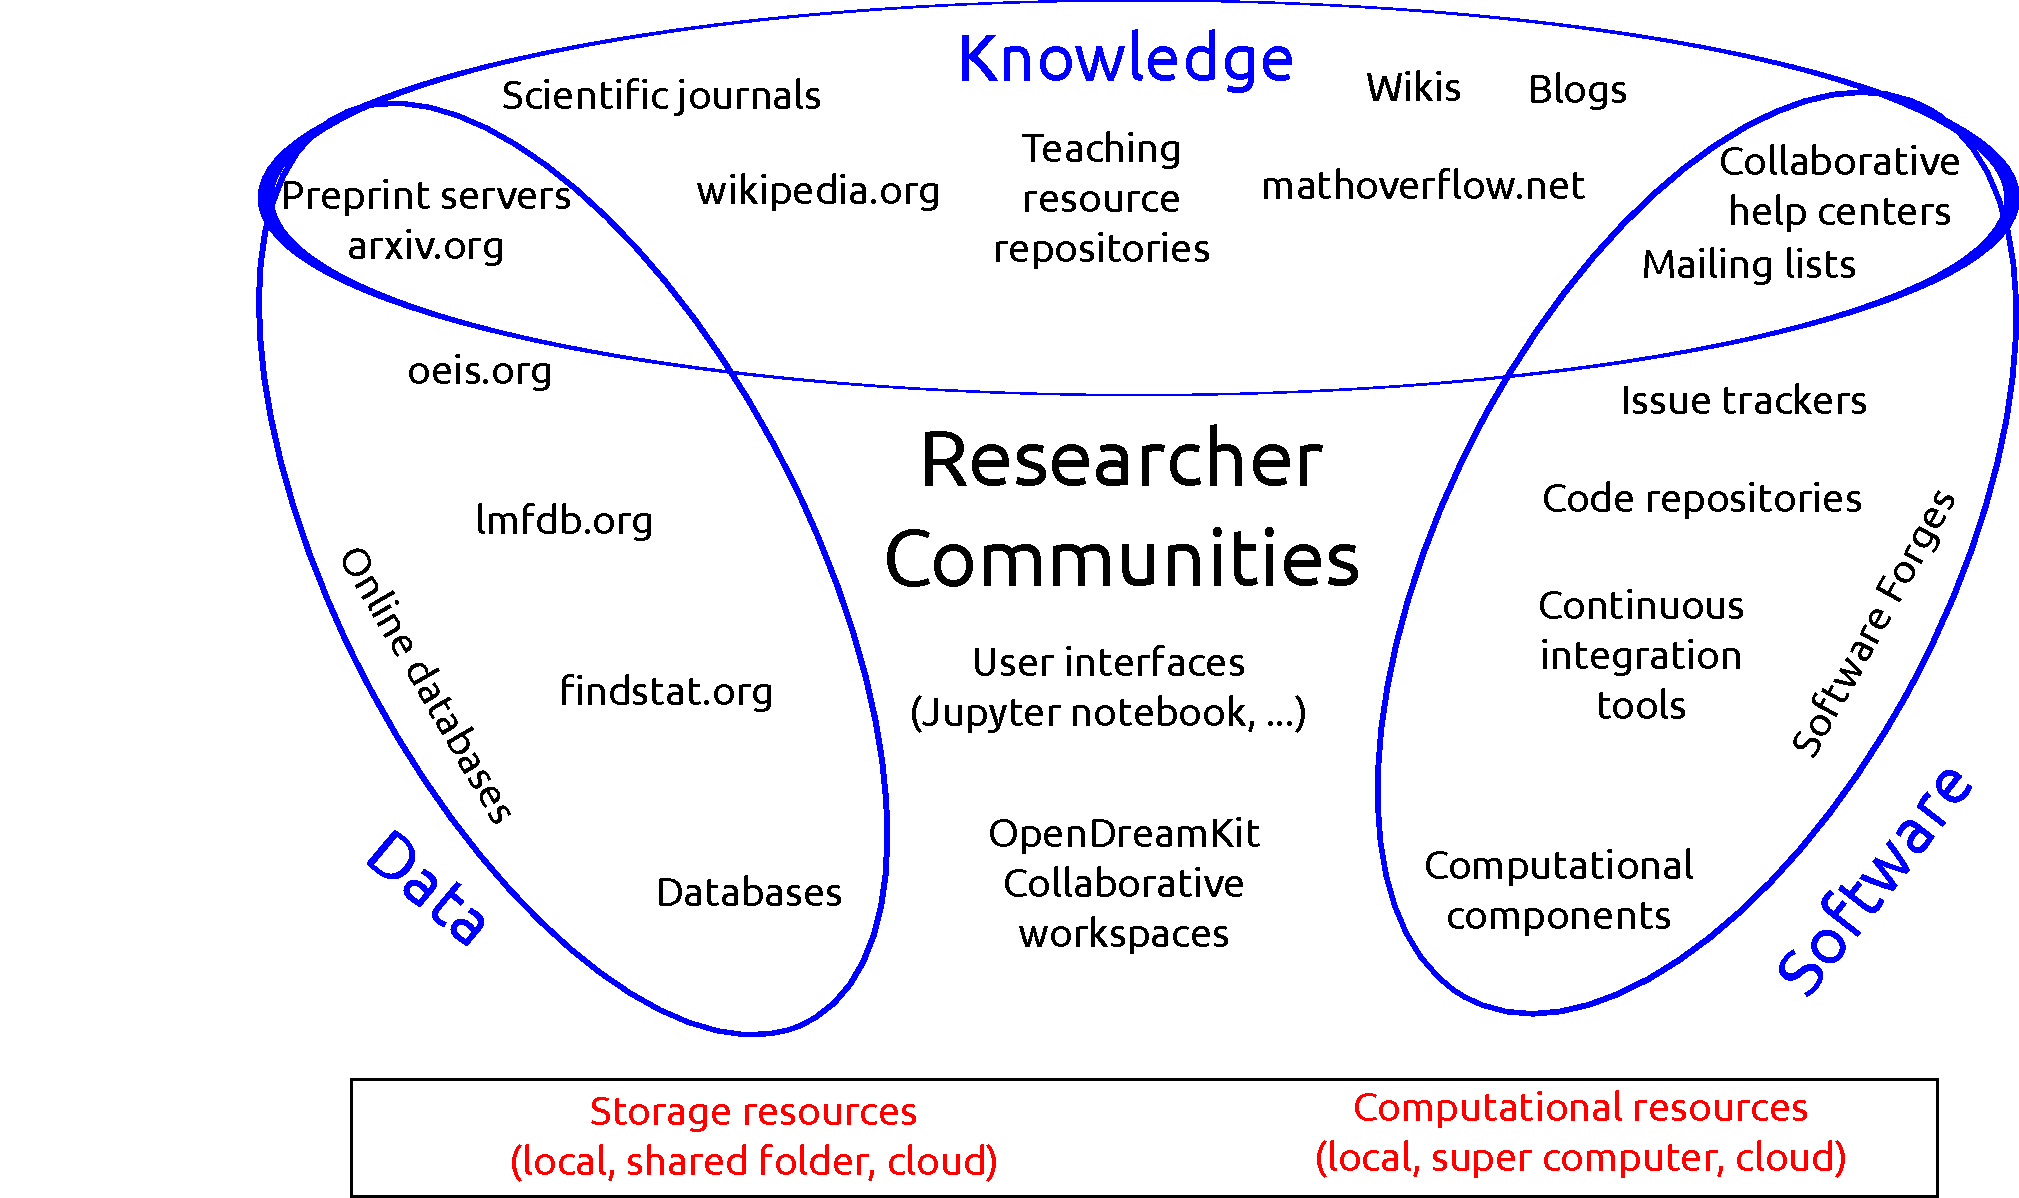
\includegraphics[width=\textwidth]{Pictures/TheBigPicture.pdf}}
  \caption{Virtual Research Environments for research in pure
    mathematics and applications.}
  \label{fig:thebigpicture}
\end{figure}

% \TODO{NT: the purpose of Figure~\ref{fig:thebigpicture} is to give a quick
%   sense of what Virtual Research Environments can be in our context,
%   and a ``big picture'' for the project. A graphic artist friend of
%   mine is going to help me improve it. I have collected here some material for her.\\\\
%   \textbf{\Large What we would like the ``big picture'' in
%     Figure~\ref{fig:thebigpicture} to highlight:}
%   \begin{description}
%   \item[This is a human centered project:] At the core: researchers and communities
%     thereof.
%   \item[The three types of information:]
%     Software, Knowledge, Data (currently in blue)\\
%     How they interact:
%     \begin{compactitem}
%     \item Knowledge help structure data and software (e.g. through ontologies)
%     \item Software produce data
%     \item Data is used by researchers to build knowledge
%     \end{compactitem}
%   \item[Physical resources:]
%     (currently in red)
%   \item[Virtual Research Environments]\ 
%     \begin{compactitem}
%     \item Researchers in Math have a long tradition of collaborating
%       on Software, Knowledge, and, up to some point, Data
%     \item For this they use a variety of collaborative tools which
%       form a loosely knit Virtual Research Environment.
%     \item \textbf{Aim 2}: make it easy for subcommunities of
%       researchers to set up custom collaborative work spaces / Virtual
%       Research Environments tailored to their needs, by combining:
%       \begin{compactitem}
%       \item Computational resources
%       \item Storage resources
%       \item Computational software components
%       \item Databases
%       \item User interfaces
%       \item Wikis-Knowledge bases (true for findstat, LMFDB): quicker
%         cycle for consolidation of information spread over
%         papers/brains
%       \end{compactitem}
%       Such VRE shall help them:
%       \begin{compactitem}
%       \item collaboratively develop software (e.g. specialized
%         libraries), data and knowledge (e.g. articles) for their
%         research projects.
%       \item contribute back this information to the larger community
%         whenever relevant.
%       \end{compactitem}
%     \end{compactitem}
%   \item[Processes:]\ \\
%     It would be interesting to depict the following processes. They
%     are indeed about collaboration and sharing (and quality control),
%     that is what \textbf{Aim 1} is to promote.
%     \begin{description}
%     \item[Software development]\ 
%       \begin{compactitem}
%       \item \emph{bug reports} and \emph{enhancement requests} emerge
%         from the community, typically through collaborative help
%         centers, and are posted on issue trackers.
%       \item \emph{Design discussions} occur on mailing lists and issue
%         trackers.
%       \item Researchers \emph{submit code} to the code repositories.
%       \item \emph{Quality control}: the code is reviewed and
%         tested by continuous integration tools.
%       \item Finally the code \emph{integrated} within computational
%         components, and used by the community.
%       \end{compactitem}
%       Researchers (as well as other users: teachers, engineers, ...)
%       interact at each step of the process.
%     \item[Scientific publication]\ 
%       \begin{compactitem}
%       \item researchers submit articles to journals and post them on
%         preprint servers;
%       \item the articles get reviewed by other researchers;
%       \item finally they are distributed back to the community
%       \end{compactitem}
%     \end{description}
%   \end{description}
%   %
%   Improvements to implement:
%   \begin{compactitem}
%   \item the findstat link does not work for me, kerning looks
%     extremely weird -- POD
%   \item LMFDB, OEIS, and findstat have a strong knowledge component as
%     well, with knowls and wikis, references, ...
%   \item arxiv is not far from a database of knowledge
%   \end{compactitem}
%   %
%   \textbf{\Large A collection of links that might give some idea of
%     the look and feel of our universe:}
%   \begin{description}
%   \item[Examples of (computational) components:]\ 
%     \begin{compactitem}
%     \item IPython: \url{http://ipython.org/}
%     \item GAP: \url{http://www.gap-system.org/}
%     \item Singular: \url{http://www.singular.uni-kl.de/}
%     \item Sage: \url{http://sagemath.org/}
%     \item \PariGP: \url{http://pari.math.u-bordeaux.fr/}
%     \item Linbox: \url{http://www.linalg.org/}
%     \end{compactitem}
%   \item[Examples of online collaborative tools]\ 
%     \begin{compactitem}
%     \item Issue tracker: \url{http://trac.sagemath.org/timeline/}
%     \item Code repository: \url{https://github.com/}
%     \item Collaborative help center: \url{http://ask.sagemath.org/}
%     \item Collaborative math site: \url{http://mathoverflow.net/}
%     \end{compactitem}
%   \item[Examples of online databases]\ 
%     \begin{compactitem}
%     \item Online databases: \url{http://oeis.org/?language=french}
%     \item LMFDB: \url{http://www.lmfdb.org/EllipticCurve/Q/14.a3}
%     \item Findstat: \url{http://www.findstat.org/}
%     \end{compactitem}
%   \item[Example of graphical material]\ 
%     \begin{compactitem}
%     \item \url{http://boxen.math.washington.edu/home/nthiery/main2014.pdf}
%     \end{compactitem}
%   \end{description}
% }


\COMMENT{Role of this section: reflecting our knowledge of the context
  + and explaining that the success of those early VRE’s, even if
  incomplete, showcases their importance and the appetite of the
  community for these kind of tools. It's exciting. We want to
  highlight the appetite rather than the need which is hard to define
  at this point}

%% \begin{center}
%%   \begin{boxedminipage}{.95\textwidth}\em
%%     \COMMENT{In short: maths needs VRE's}

%%     Our priority is the delivery of complete Virtual Research
%%     Environments (VRE). A VRE supports the entire life-cycle of
%%     computational work in mathematical research, from initial
%%     exploration to publication, teaching, and outreach. We envisage
%%     VREs as the main medium for development and deployment of
%%     mathematical research.
%%   \end{boxedminipage}
%% \end{center}

Virtual Research Environments are flexible, powerful, unified
environments for communication, distribution and implementation of
mathematical research.

Initial work shows the potential for this idea, for example, the
Virtual Research and Teaching Environment \SMC\ 
(see Section~\ref{linked-projects},  page~\pageref{sec:SMC-page})
hosting more than 10k users and 100k projects after just one year.  
\SMC is a open-source web-based hosting and web browser-based UI
solution for full access to systems such as \Sage, GAP, Singular, PARI/GP, IPython, and many
more, to the end user, and may be descibed as truly \emph{cloud}-based. 
Figure~\ref{fig:SMC-screenshot} on page~\pageref{fig:SMC-screenshot} shows an example of an SMC session.
\begin{figure}
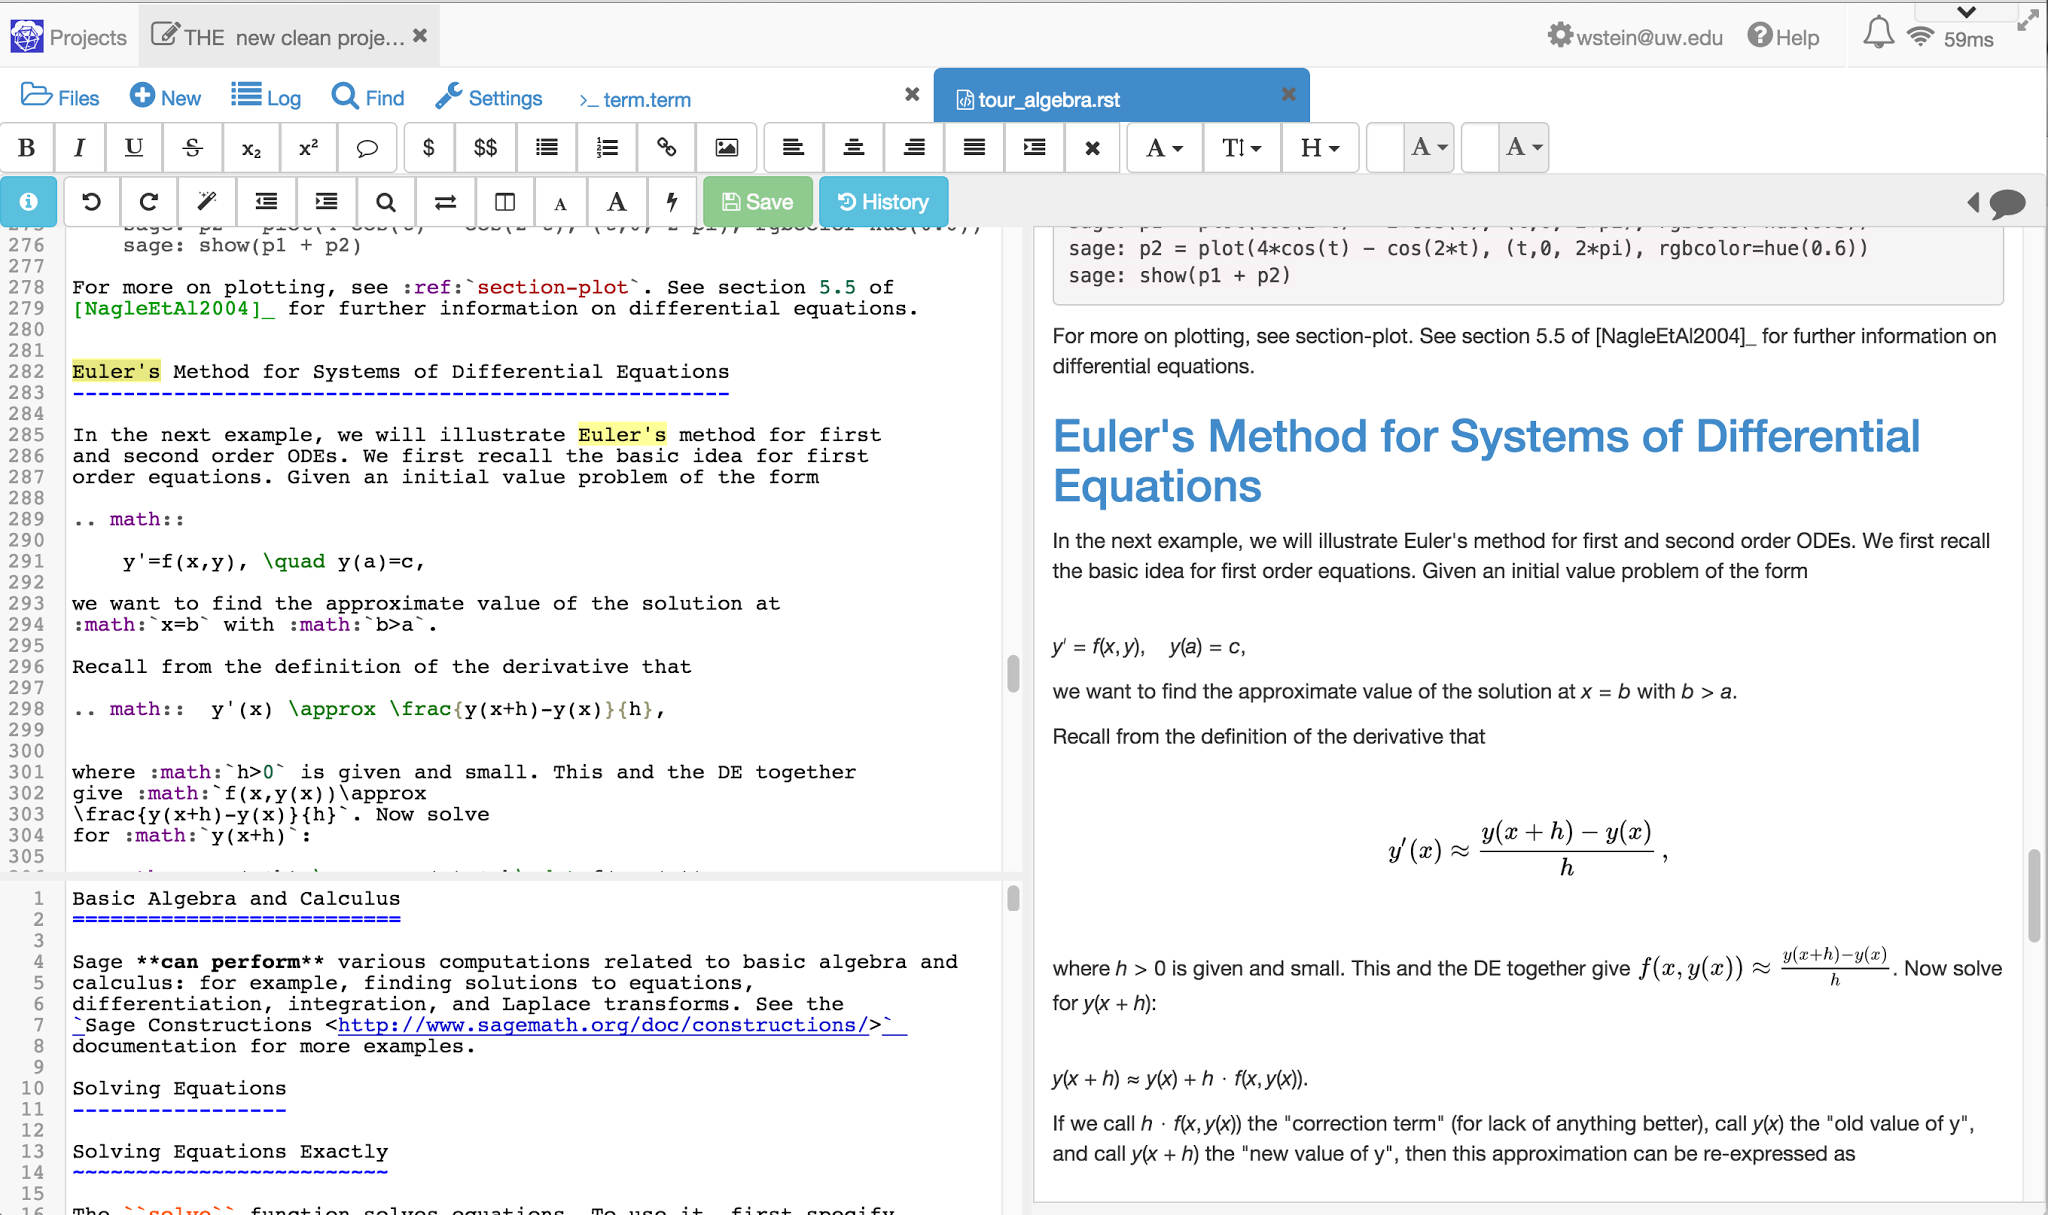
\includegraphics[width=\textwidth]{Pictures/SMC-screenshot.png}
\caption{\label{fig:SMC-screenshot} Typical \SMC\ session in a web browser} 
\end{figure}

There is widespread community interest in well-executed
\emph{integrated solutions} which can enable large-scale collaboration
on Mathematical \emph{software}, \emph{knowledge}, and
\emph{data}. This interest is also evidenced by the considerable
activity (since the inception of the internet) in a range of online
mathematical databases such as the Online Encyclopedia of Integers
Sequences, the Atlas of Finite Group Representations, and \LMFDB.
%
Other systems such as \href{http://polymathprojects.org/}{polymath}
and \href{mathoverflow.net}{MathOverflow} show the interest among
mathematicians in exploring new forms of collaboration, in particular
when the tools are well-designed and the balance of effort and reward
is correct.

Elements of a mathematical VRE can also be seen in ``everyday''
collaboration tools such as \texttt{arxiv} (sharing new mathematical
knowledge with control of provenance) \texttt{Wikipedia} (presenting
established knowledge in a consistent and linked way) and
\texttt{github}, used for collaborative paper writing as
well as software development.

\TODO{Simulagora}

\paragraph{Development models for mathematical software: a historical
  perspective}

Supporting the experimental method in mathematics requires spending
substantial resources
on software development. As the sophistication of the required
computations increased, supported by the growth of available
computational power, it became vital to distribute those efforts across
ever-larger research communities. European mathematicians have been
pioneers in this and have built up a tradition of collaborative open
source software development, that was key
to many highly successful,
open-source, community-developed specialised systems, starting with
\PariGP in Number Theory in 1979, and including \GAP in Group Theory
or \Singular in Algebraic Geometry. This was at a time when much other
scientific computing research relied on bespoke Fortran programs and used
for one calculation and then discarded.
%  \TODO{Is this quite true?
%  \url{http://en.wikipedia.org/wiki/Basic_Linear_Algebra_Subprograms}
%  says BLAS dates back from 1979 as well.}
%
%   Not quite true, but trueish. The NAG library (commercial) is another
%   possible exception

%% \COMMENT{The emergence of massive collaborative development models and
%%   tools is revolutionizing the landscape; innovation is now led by
%%   communities, not corporate software}

%% \TODO{There is redundancy below}

In that period, inter-project communication was limited by the lack of
standardisation of, and interconnection between, computers. Systems
produced remained limited
to specific research topics and often specific computer systems and
were not easily interoperable. It was left to the
corporate world to gather sufficient manpower to develop general
purpose systems that could support a broad range of engineering,
scientific and statistical mathematics, through a coherent user
interface. These companies (e.g., Wolfram, Mathworks, MapleSoft) were
mainly US-based and created a profitable industry.

% The next scale was reached in the last decade with the advent of the
% general purpose mathematical system \Sage which proved the viability
% and sustainability of the ``developed by users for users'' development
% model at the international level.

The modern environment, however, is quite different. A more connected
digital world has led to the emergence of open source software and
open development models (the so-called ``bazaar'' approach). This is
clearly exemplified in the \Sage system. \Sage is a truly
general purpose computational mathematical system. It is committed to,
and draws huge benefits from the power of open source software.
% a virtual software development environment.
It showcases the modern
reality that open source software is not just a viable alternative for
commercially produced alternatives, but it actually allows for more
rapid innovation through providing an open platform through which the
community can deploy and share advances more rapidly. \Sage demonstrates
this modern community approach to development by
delivering high quality software to researchers, teachers, and
practitioners in mathematics. It is founded on a widespread
international community of contributors and developers, and builds
successfully on a large stack of existing open source software,
ranging from the specialised computational systems mentioned above, to
\Python, a general purpose programming language that is used by
millions of programmers worldwide. This flexible, open source
architecture then allows it to rapidly assimilate new components such
as \Jupyter (formerly IPython notebook) as they are developed.

In the 1980s and 1990s the economies of scale favoured the commercial
development model for mathematical software: corporate entities could
co-locate a large body of expertise and orient it towards one
goal. This was difficult for the much larger, but naturally more
dissipated, communities of mathematical researchers. However, modern
interconnection of researchers (through the infrastructure of the
internet and collaborative development environments such as github)
start to reverse the balance of these economies. Commercial packages
can no longer develop fast enough to assimilate the innovation of the
wider mathematical community, where there is greater expertise and
manpower.

%% \TODO{The material here is somewhat redundant with the language in
%%   Objective~\ref{objective:sustainable}; see where this belongs best
%%   to. The previous section being too long, it might be good to move
%%   things here.}

\newpage

\paragraph{A unifying user interface: executable notebooks and project Jupyter}


%\subsubsection{Jupyter}
\label{sec:jupyter}

\begin{wrapfigure}{r}{0.50\textwidth}
%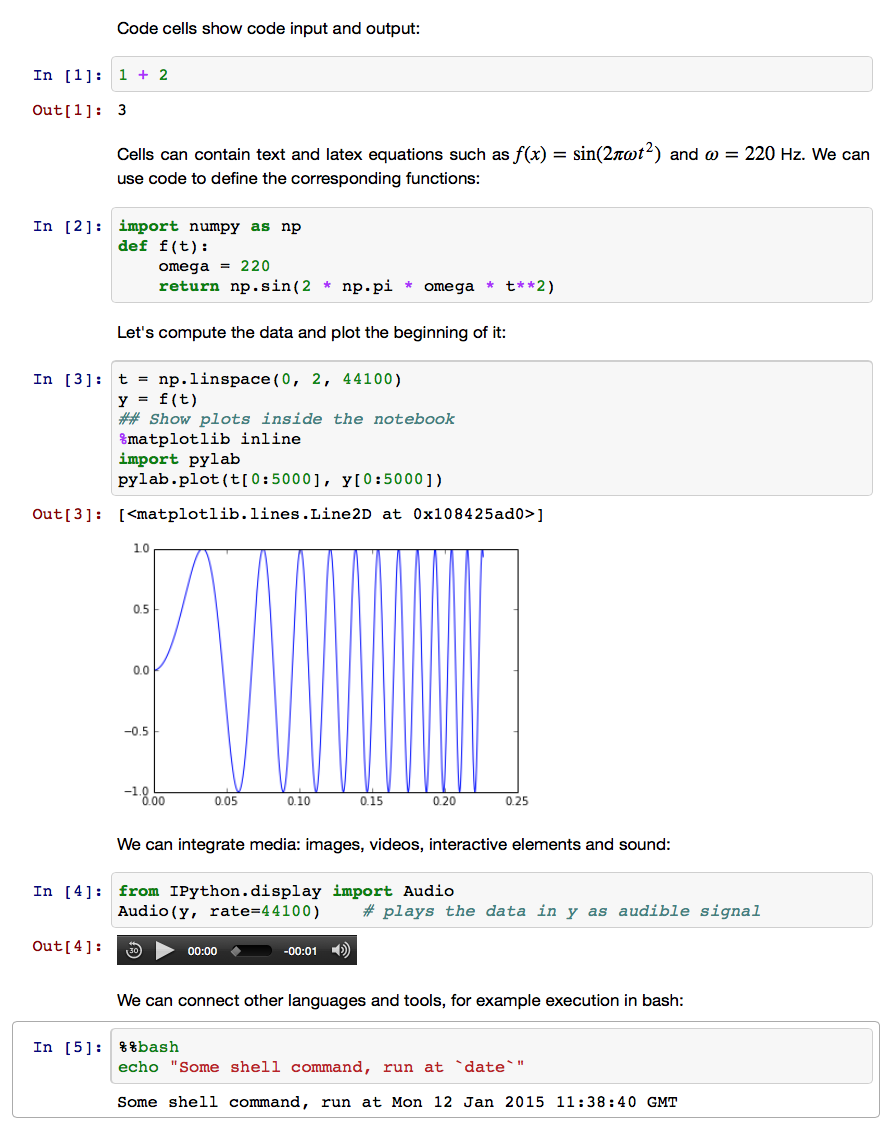
\includegraphics[scale=0.23]{Pictures/jupyterdemo1.png}
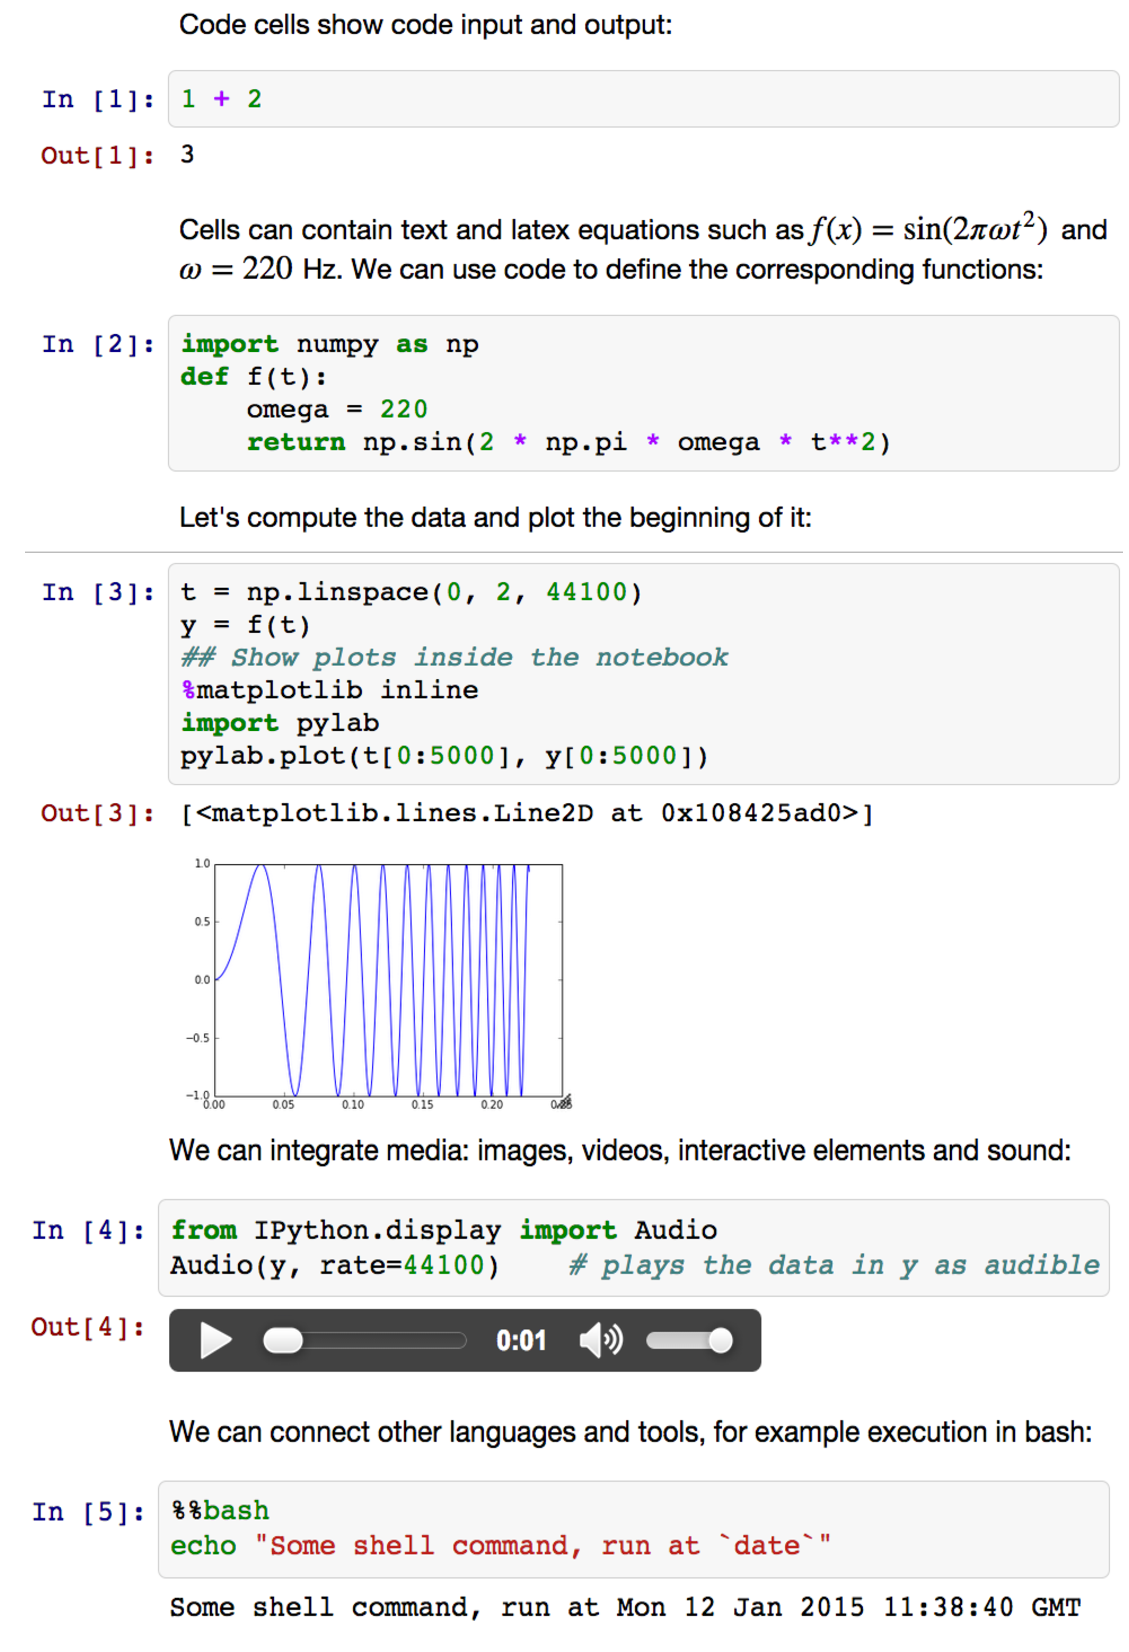
\includegraphics[width=.5\textwidth]{Pictures/jupyterdemo-largefont.pdf}
\caption{\label{fig:jupyterdemo} Self-contained \Jupyter Notebook demonstrating the concepts of cells that contain different types of material and can be executed (or updated) in arbitrary or sequential order.}
\end{wrapfigure}

Project \Jupyter \cite{Jupyter} is a set of open-source software projects for
interactive and exploratory computing emerging from \IPython \cite{IPython}. These
software projects help make scientific computing and data science
reproducible and multi-language (Python, Julia, R, Haskell, Bash, R,
\ldots). The main component offered by \Jupyter is the \Jupyter
notebook, a web-based interactive computing platform that allows users
to create data- and code-driven narratives that combine live
(re-executable) code, equations, narrative text, interactive
dashboards and other rich media.

Figure~\ref{fig:jupyterdemo} shows a Python-based sample
session. Within the Python session, all libraries available in Python
can be imported and combined flexibly, a number of interfaces between
different languages exist. Many more examples are available, for
example \cite{IPython-demo-hyperbolic-conservation-laws} and
within \cite{IPython-sload-foundation-report-2013}.

The \Jupyter notebook is being used widely in academia
(e.g. University of California, Berkeley, Stanford,
MIT, Harvard, Cambridge, Oxford, Imperial College, Southampton,
Hamburg, Paderborn, Vienna, Paris, Katowice, and Oslo) and government
(NASA JPL, LBL, KBase, White House Hackathon) as well as
industry (e.g. Google, IBM, Facebook, Oracle, Otto Group, Microsoft,
Bloomberg, JP Morgan, WhatsApp, O’Reilly, Quantopian, Logilab,
GraphLab, Enthought, Continuum, Authorea, BuzzFeed)  and
journalism (e.g. 538 and New York Times). \\
%
Because the architecture and building blocks of \Jupyter are open,
they are used to build numerous other commercial and non-profit
products and services. The \Jupyter Notebook has between 500,000 and
1.5 million individual users worldwide.

These notebook documents provide a \emph{complete} and
\emph{executable} record of a computation that can be shared with
others in a way that has not been possible before. This has led, among
other things, to a huge boost in reproducible, interactive
teaching/education documents in recent years. A paradigm that Fernando Perez, creator of the project, has referred to as ``literate computing''.\footnote{\url{http://blog.fperez.org/2013/04/literate-computing-and-computational.html}}

We will build on this technology by extending \Jupyter with new
functionality, unifying other computational tools to be usable as
components in this framework, and merging the \Sage and \Jupyter
development.  \TOWRITE{NT}{Is the 'merge' too strong a claim? Please
  correct / remove.}






\subsubsection{Approach}

In previous sections, we have analysed the diverse needs of
researchers in pure mathematics and applications, and argued that the
concept of a VRE toolkit, as proposed by \TheProject, will match those
needs, and have a considerable impact on how mathematical research is
conducted.

In this section we describe how we will realise this concept by
building on existing software components in a new way, and why
this is an ideal time to do so.
\begin{framed}
  The fundamental factor is that the last decade has witnessed the
  emergence of the necessary building blocks, all in open source:
  \begin{compactitem}
  \item Key enabling technologies: virtual machines and containers for easy
    deployment; open cloud infrastructure; web technologies
    such as MathJax or WebGL allowing powerful in-browser clients; scalable
    decentralised database software and more
  \item Computational mathematics components as described elsewhere in
    this proposal
  \item Flexible user interfaces and interactive computing environments
  \end{compactitem}
\end{framed}

The emergence of these components is itself enabled by progress in the
wider technological environment -- cheap powerful computers; fast
reliable networks; stable and advanced platforms such as JavaScript;
and more importantly and uniquely the maturation of open source
development models and collaborative tools (e.g. \texttt{github})
supporting them. This now
makes it possible to  bring together large and diverse communities of
developers, and foster large ecosystems of interoperable
components. We elaborate later in this section how this has
specifically affected the development of mathematical software in the
last decade, showcasing the sustainability of the ``by users for
users`` development models even for general purpose mathematical
computational components. These models are still not perfect on the
largest scales, and we will address this, for our purposes within the project.

\begin{framed}
  Our technical approach is to join forces with the \Jupyter project and focus on developing
  and improving building blocks that can be
  assembled and re-used flexibly to address the varied
  requirements of mathematics and the applications of mathematics in
  science and engineering, rather than creating one particular
  monolithic environment.
\end{framed}
\paragraph{Activities}

The activities of the project are planned and structured to develop
and promote \TheProject, including new research into
architectures, database techniques, parallel algorithms and the
sociology of collaborative free software development, as well as
engineering work on existing software and networking and
community-building activities.

The project inherently spans the disciplines of mathematics and
computer science, as well as bringing in results and techniques from
social sciences. Exemplar applications may also arise from areas to
which symbolic and algebraic computing is applied, such as physics,
chemistry, systems biology and engineering.


The project is divided into seven work packages. Work Package~1
(\WPref{management}) covers project management and coordination as
usual. \WPref{dissem} is our main networking activity
including community-building workshops, demonstrator applications and
direct dissemination of project results.
This covers the following topics from section E of the Work Programme:
\begin{compactitem}
\item dissemination and/or exploitation of project results and
  knowledge, contribution to socioeconomic impacts, promotion of
  innovation (\taskref{dissem}{dissemination-communication},
  \taskref{dissem}{dissemination});
\item reinforcing partnership with industry: outreach and
  dissemination activities, transfer of knowledge, activities to
  foster the use of e-infrastructures by industrial researchers,
  involvement of industrial associations in consortia or in advisory
  bodies (\taskref{dissem}{dissemination-communication},
  \taskref{dissem}{dissemination}, \taskref{dissem}{project-intro});
\item strengthening of virtual research communities
  (\taskref{dissem}{devel-workshops},\taskref{dissem}{dissemination});
\item spreading of good practices, consultancy and training courses to
  new users (\taskref{dissem}{project-intro},
  \taskref{dissem}{dissemination-of-oommf-nb-workshops});
\item exchange of personnel and training of staff
  (\taskref{dissem}{devel-workshops}).
\end{compactitem}


The remaining work packages are Joint Research Activities, dividing up
the research needed to design and implement the \TheProject and
investigate the best models for its future development. \TODO{Explain
  the rationale for the division and how they all come together at the end}

This covers the following topics from section E of the Work Programme:

\begin{compactitem}
\item higher performance methodologies and protocols, higher performance instrumentation,
  including the testing of components, subsystems, materials, techniques and dedicated
  software; (\WPref{UI}, \WPref{hpc})
\item integration of installations and infrastructures into virtual
  facilities (\WPref{component-architecture};
\item innovative solutions for data collection, management, curation
  and annotation (\WPref{dksbases});
\end{compactitem}


Additional topics addressed include effective software development and
maintenance methodologies for systems of free software systems and the
design of VREs to best support real mathematical practice.

Since the infrastructure that we are developing is free software,
there is no need for formal Service activities. All partners have
access to all the software anyway, and development and demonstration
can take place on computing resources already available to them.

\subparagraph{Networking activities}
The mathematical software community, and the various overlapping open
source software communities already have an excellent spirit of
collaboration, and excellent cultures promoting open debate, constant
improvement and common purpose. Our networking activities build on
this in essentially two directions: within the project we aim to
provide more opportunities for close collaboration and learning
from one another, in visits, code sprints, and cross-community days;
outside the project we aim to encourage more users of mathematical
computation to join this ``community-of-communities'' through our open
workshops, training events and demonstrator applications.



\subparagraph{Joint Research Activities} The joint research activities are defined by our
vision for \TheProject and match up with the work packages defined in
the implementation section:
\WPref{component-architecture} defines the
requirements for a component to be part of the kit, \WPref{UI}, \WPref{hpc} and
\WPref{dksbases} address limitations of current components, or areas where they have
become out of date and \WPref{dissem} is key to our goal to produce systems that
address the end-user needs.


By focusing on a toolkit rather than a monolithic VRE, and by
concentrating the efforts on improving and unifying existing general
purpose building blocks, \TheProject
will simultaneously maximise sustainability and broad impact. Although
the primary target users are \emph{researchers in
  mathematics}, the beneficiaries include users of components such as
\Jupyter in  scientific
computing, physics, chemistry, biology, engineering, medicine, earth
sciences and geography, and  teachers
and practitioners in industry as well as researchers.
Users of many of the component systems will also benefit from our
improvements even if they do not choose to use \TheProject VRE, since
those components will be updated and improved. We will also perform
important research into open
development models that will benefit academia and many highly
innovative SME's.


\subsubsection{Benefits of this approach}

Throughout this project we will reuse and extend existing open source
systems. By doing this, we ensure that \TheProject will benefit from future open
source contributions during and beyond the lifetime of the project. By
unifying tools with overlapping functionality, such as \Jupyter and
\Sage, we focus the effort of the computational community onto
\TheProject, producing additional economies of scale. Finally, thanks
to the ``by users for users`` model, the development will be steered
by the actual needs of the community.

The net effect of this is that \TheProject will include far more
capabilities and code than could possibly be developed within a single
research project, and will continue to accrue additional capabilities
from its users as it is used. The investment in this project will be
greatly amplified by these factors and the impact and sustainability
greatly increased.


\subsubsection{Demonstrators}

\TOWRITE{NT}{Simulagora}


To confirm the usability of our software tools, and demonstrate their
value to potential academic and industrial users groups, we plan three
demonstrator projects. These will be developed as soon as the
necessary components are available to give early feedback and then
refined and maintained during the remainder of the project to
demonstrate the increasing scope and reliability of \TheProject.


\paragraph{Demonstrator: Interactive Books} ---
In \taskref{dissem}{ibook}  we will produce a series of interactive books
that can be read, executed, modified and explored within the
\TheProject VREs. This will demonstrate the collaboration and
document-handling capabilities of \TheProject and the ability to link
presentation to computation. The books will target students, an
audience familiar with modern web applications, but with traditional
computational tools. Evaluation of the acceptance of these books with
provide valuable feedback on our user interface components.

\begin{figure}
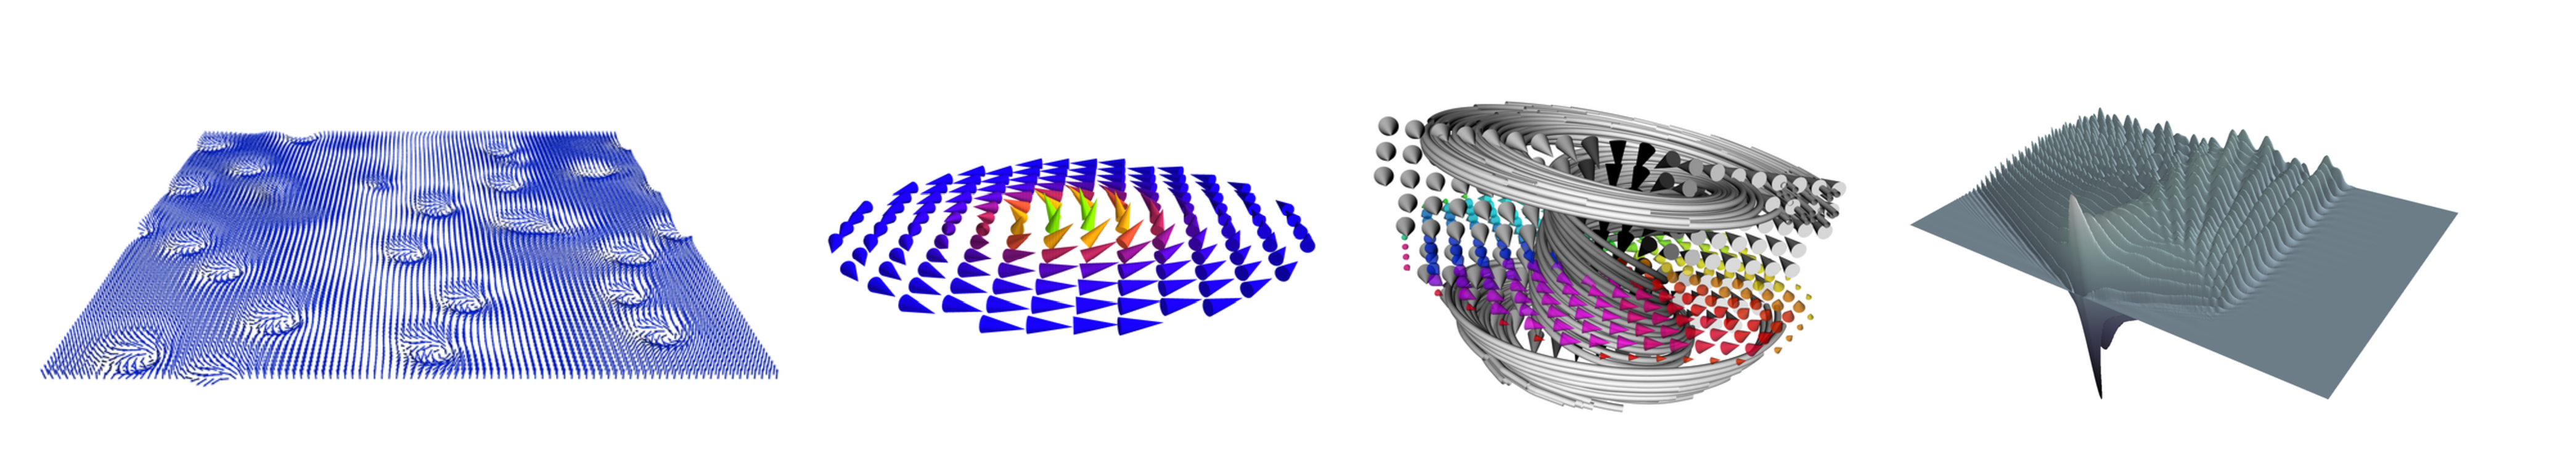
\includegraphics[width=1.0\textwidth]{Pictures/micromagnetic-and-3d-vis-4x1.pdf}
\caption{\label{fig:3d-plots} A selection of typical visualisation patterns often required in science and engineering. From left to right: a 3d vector field on a 2d domain, a 3d vector field coloured with another scalar field on a 2d domain, a 3d vectorfield on a 3d domain with streamlines, and scalar field plotted on a 2d domain.}
\end{figure}

\paragraph{Demonstrator: Micromagnetic VRE}
\label{sec:introduction-micromagnetic-vre-demonstrator} In
\taskref{UI}{oommf-py-ipython-attributes} we will build
a sample VRE targetting a specific research community, that of \textit{micromagnetics}.

Micromagnetics deals with the behaviour of
magnetisation at length scales of the order of
micrometers and below. It is widely used in the research and
development of magnetic data storage media and devices, for magnetic
sensing, permanent magnets and healthcare applications such as cancer
treatment and diagnostics. Figure~\ref{fig:3d-plots} shows some micromagnetic simulation results.
Researchers needing to carry out simulations in this area often do not
have  extensive computational background; they may be
material scientists, engineers and physicists that
interpreting  experiments and designing new devices. Industrial users include Seagate, Hitachi,
TDK, Samsung, Bosch and Toyota.


We will embed the most popular micromagnetic
simulation software (Object Oriented MicroMagnetic Framework
\cite{OOMMF-url}, which has over 1800 citations) within a micromagnetic VRE, complemented by other
components that add value, including notebook user interfaces,
replacing the current text driven, unautomated and error-prone workflow.

We will evaluate this demonstrator application in 
\taskref{social-aspects}{oommf-nb-evaluation}, immediately feeding
results back into the \TheProject work. This will also
be a case study for the sustainability of the approach and tool beyond
the life time of this H2020 project.

\paragraph{Demonstrator: Computational Mathematics Resource Indexing
Service}

In \taskref{dissem}{index-librorum-salvificorum} 
we will demonstrate the ability to build persistemnt highly-linked
web-based services using \TheProject by developing a unified index of
components and documents relevant to \TheProject. This will test
elements such as cloud interaction and internationalisation, and our
abvility to provide a uniform mathematical view of diverse
components. It will also serve
to advertise the range of components available.




\subsubsection{Specific requests of the call}

\paragraph{Use of Existing Basic Services}
This will be addressed primarily in work packages \WPref{component-architecture},
\WPref{dksbases} and \WPref{hpc}. Our architecture will include interfaces to standard
APIs for cloud provisioning, authentication, cloud storage, HPC scheduling and so
forth. Actual VREs will be deployed by users integrating those with specialist tools
according to the needs of their projects. \COMMENT{weak}

\paragraph{Gender analysis}

All partners will follow inclusive practices in recruiting staff for this project, in
inviting the community to our workshops and outreach events and in choosing users to
evaluate our demonstrator applications. We will consult with the Head of Equality and
Diversity at St Andrews, about any known gender differences in collaborative working and
ensure that our collaborative tools properly support open, equitable and inclusive
patterns of cooperation. This will be reported in deliverable \delivref{management}{ipr}.

\paragraph{Service discovery}

The \TheProject web pages (\taskref{dissem}{dissemination-communication}) and the
dedicated training portal (\taskref{dissem}{training-portal}) will
provide a central point of service discovery, providing a directory to
all components, demonstrators, online services, protocol and interface
specifications, software and other project activities and outputs.

\TOWRITE{NT}{Happy with the above Service discovery snippet?}

%%  \TheProject aims to create a framework to make the
%% systems interoperable and synergistic and to give working mathematicians full access to
%% the potential spanned by already-existing systems. Essentially every node in
%% Figure~\ref{fig:thebigpicture} represents a user community, so \TheProject is at its heart
%% a project that also combines researchers and communities.


%% \subsubsection{Old material}

%% \TODO{What the proposal is about}
%% This proposal is about providing mathematicians with the tools to
%% carry out and communicate their research effectively. It will ensure that ideas are
%% distributed and discussed as widely as possible to enable rapid
%% assimilation of these ideas into the pipeline of innovation. Our aim
%% is to develop an ecosystem that exploits the modern computing
%% infrastructure to streamline development and deployment of
%% mathematical advances. We will ensure that the societal benefit of
%% these advances is realized in the shortest possible timescale.

%% This proposal is about supporting the next generation of innovation in
%% the mathematical computing ecosystem. It is a Europe-wide
%% collaboration that assimilates a leading body mathematicians and
%% computational researchers with a track record of delivering innovative
%% open source software solutions.

%% In keeping with the \Sage strategy, a major focus is on reusing and
%% improving existing components, and reaching toward larger communities
%% whenever possible.

%% \begin{center}
%%   \begin{boxedminipage}{.95\textwidth}\em
%%     \COMMENT{Short description of the consortium}

%%     To achieve this aim, \TheProject brings together lead developers
%%     and experts from existing mathematical computational components
%%     (\Linbox, \GAP, \Sage, \Singular), existing Virtual Research
%%     Environments (\SMC, \Simulagora), online mathematical databases
%%     (\LMFDB), mathematics knowledge portals (\MathHub) and general
%%     purpose interactive computing components (\Jupyter).

%%     \TODO{Most of the participants are themselves primary users of the
%%       infrastructure, with a long track record of community building
%%       and dissemination. Thus the governance will naturally be steered
%%       by users needs.}
%%   \end{boxedminipage}
%% \end{center}


%%   Chunks of language that we might want to recycle above:
%%   \begin{compactenum}[\em i)\rm]
%%   \item \TheProject will attack all those challenges upfront, while
%%     consolidating Europe's leading position in this field.
%%   \item innovate virtual research environment (VRE) development:
%%     instead of building an essentially monolithic system like
%%     Mathematica or Maple, we will build an open framework for Math
%%     VREs, which can be extended by plugins and experimented on as
%%     needed, and
%%   \item wrest the initiative in the space of computational mathematics
%%     from the corporate world into the open source research/innovation
%%     community, which is traditionally strong in Europe.
%% \end{compactenum}

\subsubsection{Linked research and innovation activities}\label{linked-projects}

\eucommentary{Describe any national or international research and
  innovation activities which will be linked with the project,
  especially where the outputs from these will feed into the project;}

\TODO{For each item below, write a paragraph describing the project
  and one describing how it connects with this proposal}

\paragraph{DFG Priority Project SPP 1489}
\url{computeralgebra.de}

The SPP1489 ``Algorithmic and Experimental Methods in Algebra, Geometry, and
Number Theory'' is a nationwide Priority Project of the German Research Council DFG
which commenced in July  2010 and will end in June 2016. The focus of the programme
is on the interactions between computer algebra and algebraic geometry, number theory,
and group theory. It combines expertise at all levels of research in computer algebra,
be it the design of algorithms, the implementation of algorithms, the application
of algorithms, or the creation of mathematical databases. The goal of SPP1489 is to
considerably further the algorithmic and experimental methods in the afore mentioned
disciplines, to combine the different methods across boundaries between the disciplines,
and to apply them to central questions in theory and praxis. A fundamental concern of the
programme is the further development of open source
computer algebra systems with origins in Germany, which in
the framework of different projects will be cross-linked on
different levels. Of particular interest are interactions with application areas inside
and outside of mathematics such as system- and control theory, coding
theory, cryptography, CAD, algebraic combinatorics, and algebraic
statistics as well as hybrid methods which combine numerical and
symbolic approaches.

The work in the SPP1489 has established effective communication channels between the core
developers of different computer algebra systems. It is a showcase project for several
objectives of this proposal (such as community building and fostering a sustainable
ecosystem of interoperable open source components).  The experience made in parallelizing
mathematical software will be crucial for Work package \WPref{component-architecture}.


\paragraph{IPython/Jupyter grant from the Alfred P. Sloan foundation}
\url{http://ipython.org/sloan-grant.html}

The IPython project received a \$1.15M grant from the Alfred P. Sloan
foundation that is supporting IPython development for two years
(1/1/2013-12/31/2014), in particular at the University of California,
Berkeley and California Polytechnic State University, San Luis Obispo.
This grant enabled the project to focus on developing the IPython
Notebook as a general tool for scientific and technical computing that
is open, collaborative and reproducible. This goes a long way toward
the aims \TODO{... and ...} of \TheProject, especially given the current
rapid evolution of IPython toward its language agnostic avatar
Jupyter.

\TheProject will build on the outcome of the Sloan grant, and further
develop the critical IPython/Jupyter component in close collaboration
with the IPython/Jupyter team. In particular, we plan to hire some of
the European developers that are currently funded by the Sloan grant
to work in California and wish to later return to Europe.

\paragraph{NSF SI2-SSE OCI-1147247}

%\SageCombinat is a subproject of \Sage whose mission is "to improve
%\Sage as an extensible toolbox for computer exploration in (algebraic)
%combinatorics, and foster code sharing between researchers in this
%area".

The OCI-1147247 Collaborative Research grant ``Sage-Combinat:
Developing and Sharing Open Source Software for Algebraic
Combinatorics'' is a project funded by the National Science Foundation
from June 2012 to May 2015. The grant supports the development of
\SageCombinat, on the USA side, and in areas relevant to the ongoing
research of the participants (symmetric functions, Macdonald
polynomials for arbitrary Cartan types, crystals, rigged
configurations and combinatorial R-matrices, affine Weyl groups and
Hecke algebras, cluster algebras, posets, ...), together with relevant
underlying infrastructure. The grant funds a yearly Sage Days
workshop, and cofunded two others at ICERM and Orsay respectively. The
grant also funds a dedicated software development and computation
server for \SageCombinat, hosted in the \Sage computation farm in
Seattle. Emphasis is placed on the development of thematic tutorials
that make the code accessible to new users. The grant also funds
graduate student RA support, curriculum development, and other
mentoring.

Thiéry and Stein, respectively coordinator and in the tentative
advisory board of \TheProject,
are respectively foreign senior participant and PI of this NSF grant.
It funded, through them,
some of the development of \SMC as well as of the category framework
in \Sage; both are key assets for this proposal. The workshop and
outreach actions pursued by this NSF grant have proven to be potent
tools for connecting researchers and recruiting users and
developers. One of the role of this proposal is to support similar
community building in Europe.

\paragraph{Open Archive of Formalizations (DFG)} The German Science Foundation (DFG) has
funded a three-year project (OAF) on the development of a integrated knowledge base of
formal mathematics. The project builds on the LATIN project (DFG) which developed a
foundation-independent metalogical framework for representing and interrelating theorem
prover logics based on the OMDoc/MMT format. In the OAF project, the LATIN Framework is
extended to a system that allows combine the most important theorem prover logics in one
system (MathHub/OAF).  The PIs of the OAF project (Kohlhase/Rabe) are members of the
\TheProject Consortium.


\paragraph{HPAC grant from the A.N.R.}

The French national research agency ANR has funded a 4 years project
on High Performance Algebraic Computing (HPAC) focused on the
development of parallel exact linear algebra. The consortium gathers
research groups from LIP6 (Paris 6), LIRMM (Montpellier), LIP (Lyon)
and LIG and LJK (Grenoble). The main goals of the project is to first
develop high performance exact linear algebra kernels with dedicated
parallel runtime, propose a domain specific language for the
parallelisation of exact linear algebra libraries and their
composition, invent new algorithmic solutions for large scale
parallelisations. The output of the project is then twofolds: new
computational challenges arising in algebraic cryptanalysis will be
addressed, and the open-source libraries maintained by each group will
not only integrate these advances, but will expose them in a close
integration to high level computer algebra softwares. In this process,
\Sage will start benefitting from the new shared-memory parallel code
of \Linbox for the linear algebra over a finite field.  The scope of
this project is mostly focused on shared memory parallelism (except
for some challenge computations). Addressing distributed and
heterogeneous infrastructures is the next step after this project,
that is be addressed in work-package 5 of the this proposal.


\paragraph{RADIANT Grant from EU FP7-HEALTH (ref 305636)}
\url{http://radiant-project.eu/}

This EU funded proposal focuses on making available computational and
mathematical models to the computational biology communities as
rapidly as they are developed with a particular focus on high
throughput sequencing techniques. The rapid development of sensorics
technology in the biological sciences results in mathematical
challenges in the data analysis. To address these challenges in a
timely manner collaborative frameworks for mathematical and
computational modelling are required. \TheProject provides the
framework for pipeline delivery of methodologies to end users through
approachable IPython/Jupyter notebooks.

% for an example see: http://nbviewer.ipython.org/github/SheffieldML/notebook/blob/master/compbio/index.ipynb

\paragraph{Cubicweb} \url{http://www.cubicweb.org}

Logilab has been developing CubicWeb since 2001 as FLOSS (Free Libre Open
Source Software). CubicWeb is a semantic web framework, that allows to
build web applications and web services from an ontology. CubicWeb
could be used in \TheProject to build mathematical databases dynamically
that will store data, knowledge and software.

\paragraph{Math Search (Leibniz Foundation)} The Leibniz foundation has funded a
three-year project on search in mathematical information systems. The project is
undertaken by FIZ Karlsruhe (the publisher of the Zentralblatt Math Database) and
\site{JU}. The project has developed a formula/keyword search engine that is in production
use for Zentralblatt (see \url{https://zbmath.org/formulae/}).

\paragraph{Simulagora} \url{http://www.simulagora.com}

Logilab is maintaining Simulagora, a software as a service (SaaS) that builds
on free software (FLOSS) to provide its users with a Virtual Research Environment
(VRE) that greatly guarantees traceability and reproducibility as well as
facilitates group collaboration. Logilab will bring its experience of Simulagora
to \TheProject and feed back to Simulagora many of the deliverables available
under a free license.

\paragraph{Sage Math Cloud} \url{https://cloud.sagemath.com/} \label{sec:SMC-page}

\SMC provides a collaborative online environment for students,
teachers and researchers to interact with \Sage and with each
other. It has \Sage and \IPython worksheets, powerful \LATEX editing
features and a full \Linux shell, all accessible from a standard
web browser. Its main design feature is to enable and promote
collaboration between groups of users. It is for example a natural
place to host a course, allowing teachers to collaborate with their
students using modern tools like \Sage and \LATEX, with facilities for
real-time communication through chat, video, and shared editing of
documents, programs and worksheets; course material can be provided as
worksheets, assignments can be distributed, collected, and returned as
well. Launched in 2013, \SMC presently hosts over 100,000 projects and
10,000 weekly active users. This fast adoption by a wide variety of
users demonstrates the relevance and the long term impact this kind of
collaborative environments can have.

Technically speaking, \SMC is a specific open-source cloud-based
Virtual Research and Teaching Environment for mathematics developed
since 2013 under the lead of William Stein, with funding from the NSF,
and Google's Education Grant program.
It's currently deployed partly at the University of Washington at
Seattle, and there is a business plan for commercial support for
courses.


%  It's currently deployed at the
% University of Washington at Seattle, with a business plan in the work
% for commercial support for massive on line courses, subsidizing a free
% service for all other academic usage and some further \Sage
% development.

In comparison \TheProject focuses on open source building blocks and
architecture to easily set up and deploy custom Virtual Research
Environments. On the one hand, \SMC will serve as prototype for
\TheProject, paving the way and showcasing important features from the
users perspective. On the other hand, basically each and every task
undertaken in \TheProject will be of benefit to \SMC.

% \paragraph{FLINT grant?}

\paragraph{LMFDB grant}\url{http://www2.warwick.ac.uk/fac/sci/maths/people/staff/john_cremona/lmf}

The L-functions and Modular Forms Database (LMFDB) project originated
at a meeting at The American Institute for Mathematics (AIM) in 2007.
As well as providing a central repository of data as a resource for
researchers in number theory, through its website \url{www.lmfdb.org},
the LMFDB provides a modern handbook of L-functions and related
objects, including tables, formulas, links and references.  The LMFDB
has been funded by the NSF (2008-2012, \$1M) and by EPSRC (2013-2019)
through a £2.2M Programme Grant, PI Prof.~J.~E.~Cremona (Warwick).

Almost all contributors to the LMFDB project are pure mathematicians,
with good computational skills, but not professional programmers or
software developers.  The LMFDB hence needs to broaden the support it
can call upon from software professionals, for the computation of
number-theoretic data and also to support database management and
enhance the website user interface.  The codebase of the LMFDB project
is entirely open source and hosted at GitHub
\url[https://github.com/LMFDB/lmfdb], written in Python with
specialist modules such as flask and pymongo to manage the website and
database interface, and \Sage\ for higher-level mathematical
computations.  It also implements ``Knowls''
(\url{http://www.aimath.org/knowlepedia/}), a very fruitful method of
presenting mathematical knowledge which have been an unexpected
spin-off, now used in many websites unrelated to the LMFDB.

The LMFDB project would benefit greatly from collaboration with
\TheProject by connecting with a wider pool of experts in computer
science.  The proposed joint workshops between the LMFDB and
\TheProject will stimulate and enable collaboration.  As a leading
example of the use of databases in mathematical research, the LMFDB
will provide \TheProject\ with a real large-scale prototype around
which to develop new ideas about the design and implementation of such
databases and their associated software.  The feasibility of such
collaboration was successfully tried at a workshop at ICMS (Edinburgh)
in 2013 on ``Online databases: from L-functions to combinatorics'',
sponsored by the NSF, AIM and the ICMS.

\paragraph{``ACCORD: Algorithms for Making Complex Decisions on Structured Domains''}
is Edith Elkind's ERC Starter Grant
awarded in 2014, and to be started in March 2015. It
will develop theoretic tools for analysing and improving situations
arising in collaborative environments.
It can be viewed as a interdisciplinary project, bringing together methods from
computer science, game theory, and economics and political science
to quantify complex behaviour of social interactions, and engineer
positive outcomes by designing appropriate mechanisms.
In particular, it aims to develop a suite of preference aggregation procedures with complex outputs (i.e.,
partial orders satisfying user-defined structural restrictions) that admit efficient algorithms on realistic
inputs and are computationally resistant to dishonest behavior, and to identify a set of guiding
principles that can be used to choose an appropriate procedure from this suite for a specific decision-making
scenario.

\TheProject\ VRE appears to be a natural testing ground and a potential virtual
laboratory for developing and testing ideas and tools developed, within the
framework of the grant, on in a ``real life'' situation, and the collaboration
will be mutually beneficial for both projects.


\paragraph{``MathSoMac: The Social Machine of Mathematics'', EPSRC EP/K040251/2}
is Ursula Martin's EPSRC Senior Fellowship grant, started in
2014 and to be running for 4 years. It brings rigorous methods from social
sciences into studying of the crowdsourcing, e.g., large-scale online
collaboration, phenomenon in mathematical sciences.  Most striking is this
regard are recent large scale collaborations, such as the Polymath projects led
by Fields medallists Gowers and Tao, the collaboration on homotopy type theory
led by Fields medallist Voevedsky and others.  Martin’s project will develop
new paradigms to understand these, and new tools to support them, within the
framework provided by the larger EPSRC collaboration, SOCIAM, 2013-2018. SOCIAM
aims to understand the phenomenon of social machines, defined as purposeful
human interactions on the web, and to enable the effective co-ordination and
deployment of the burgeoning ecosystem of social machines currently available.
SOCIAM aims to answer questions such as how individuals are incentivised to
take part, how communities develop and mature, and how the speed and quality of
results can be optimised. A mathematical example is provided by OEIS, the
online Encyclopedia of Integer Sequences, where it is volunteer social
mechanisms that determine the nature of the data available and the reliability
and reproducibility of outcomes.  SOCIAM in turn builds on previous work in
Oxford (De Roure, Goble and others) on VREs, such as MyExperiment.

\TheProject\ and VREs in general are natural objects to investigate
within the framework of this grant, and conclusions drawn would lead to better understanding
of the ways VREs function. This has important potential benefits for \TheProject, and
vice versa.

%\paragraph{Findstat?}

%\paragraph{KWARC group}

\paragraph{SCIEnce: Symbolic Computation Infrastructure for Europe}
(FP6 eRII3-CT-026133, 2006--2011) was coordinated by the University
of St Andrews (PI Prof Steve Linton) and tackled the fragmentation of the
European community of researchers in, and users of, symbolic computation.
Among the nine partners were four major system developers (of \GAP,
\Maple, \MuPAD and \KANT), an international research institute (RISC-Linz)
and other groups with specialist expertise. Project activities
included symbolic web services, system composability, symbolic
grid and cloud computing and a program of visits, workshops and
summer schools. One important outcome was a new protocol \SCSCP,
now used well beyond the original project.

\paragraph{HPCGAP: High Performance Computational Algebra and
Discrete Mathematics} (EP/G055181, 2009--2014) was a 4-site project
coordinated by the University of St Andrews (PI Prof Steve Linton). It aimed
at reengineering GAP to support simple, safe and efficient parallel
programming on a range of systems from multicore laptops and desktops,
through departmental and university clusters to HPC systems. By the
end of the project, we had adapted a complex system including a
language runtime and over 400 000 lines of interpreted code to enable
safe and efficient parallel programs. The proposed project is very timely as
the multi-threaded version of GAP is becoming mainstream, and users and
package developers need training and support to parallelise their code.

\paragraph{CoDiMa} is a new EPSRC funded Collaborative Computational Project
in the area of {\em Co}mputational {\em Di}screte {\em Ma}thematics (EP/M022641/1).
It will begin in 2015 and will be aimed at \GAP and \Sage community-building
activities in the UK, involving a programme of short research visits, workshops
and training events. Through CoDiMa, we will have an excellent opportunity to
interact with UK user and developer communities of \GAP and \Sage in order to
to collect feedback about their requirements and to inform them about \TheProject
outcomes.

\paragraph{Doctoral Training Centre in Next Generation Computational Modelling}
\url{http://ngcm.soton.ac.uk} The Doctoral Training Centre in Next
Generation Computational Modelling is a \euro{12}million investment,
jointly funded by the UK's Engineering and Physical Sciences Research
Council (EPSRC), the University of Southampton and 50 industry
partners. Its mission is to improve professionalism, simulation
software and exploitation of emerging hardware to support
Computational Science and Engineering. The centre will train about 75
PhD students and is funded to run from 2013 to 2022.

The centre has chosen the \Jupyter Notebook as the key tool used in
its teaching programme, and runs a programme to improve and
disseminate best-practice in computational science. The centre's PhD
students will be natural contributors, testers, and target audience
for dissemination of \TheProject and its research results. Hans
Fangohr (USO) is the director of this doctoral training centre.


%%% Local Variables:
%%% mode: latex
%%% TeX-master: "proposal"
%%% End:

%  LocalWords:  eucommentary programme authorisation includegraphics textwidth textbf WPs
%  LocalWords:  thebigpicture subcommunities findstat emph emph knowls IPython Linbox ce
%  LocalWords:  clearpage subsubsection Swinnerton-Dyer Millenium desingularization Serre
%  LocalWords:  Hironaka algorithmization Villamayor Serre's Mestre Simulagora Wakari.io
%  LocalWords:  tmpnb computeralgebra.de Jupyter TOWRITE SageCombinat Sage-Combinat Weyl
%  LocalWords:  Macdonald Cartan cofunded Thiéry sensorics modelling Logilab cubicweb les
%  LocalWords:  github pymongo boxedminipage compactitem mathcal compactenum EPrint qu'il
%  LocalWords:  Feit-Thomson minitoc planetmath.org Borcherds figure-vre.tex MathJax faut
% -*-mode: LaTeX; coding: utf-8;-*-
%  LocalWords:  mathoverflow.net texttt dissem pouvoir composants calcul rendre sur une
%  LocalWords:  performants gamme maximising Mathworks favoured UMs Libre Elkind's Gowers
%  LocalWords:  analysing behaviour Voevedsky Roure incentivised optimised Encyclopeadia
%  LocalWords:  Goble composability parallelise mputational screte utf-8 realise maximise
%  LocalWords:  emphasised pageref superseeker specialised trueish standardisation WPref
%  LocalWords:  taskref devel-workshops dissemination-of-oommf-nb-workshops hpc dksbases
%  LocalWords:  delivref ipr Fangohr


\draftpage
% ---------------------------------------------------------------------------
%  Section 1.4: Ambition
% ---------------------------------------------------------------------------
\TOWRITE{ALL}{Proofread 1.4 Ambition pass 2}

\subsection{Ambition}

\eucommentary{1-2 pages}

\eucommentary{-- Describe the advance your proposal would provide beyond the
state-of-the-art, and the extent the proposed work is ambitious. Your answer
could refer to the ground-breaking nature of the objectives, concepts
involved, issues and problems to be addressed, and approaches and methods to be used.\\
-- Describe the innovation potential which the proposal represents. Where relevant, refer to
products and services already available, e.g. in existing
e-Infrastructures.}

For most pure mathematicians using computational tools in their
research, the state of the art at the start of 2015 still consists of
a collection of
separate programs, each of which must be installed individually on their
desktop or laptop computer, respecting a complicated set of interdependencies.
Alternatively, software may be installed for them on a
departmental server or cluster, and used via a text- or browser-based remote
login. The software performs computations (using a variety of excellent
implementations of extremely sophisticated algorithms), with inputs and
outputs usually in a bespoke text-based format.
Multiple computations involved in producing a mathematical
result must be managed by editing, naming and filing multiple scripts
or programs, and there is no automatic support for rerunning
computations to check for human or algorithmic error. The results of
computations are incorporated into publications using cut-and-paste, and
collaboration is mostly done through exchange of programs and data by email,
shared general-purpose file servers or, rarely, a service such as
GitHub. Amongst other problems,  this approach creates a serious
obstacle to the reproducibility
of published computational experiments both by other researchers and
the authors themselves at a later time.
% see e.g. "Case Studies and Challenges in Reproducibility in the
% Computational Sciences", http://arxiv.org/abs/1408.2123, submitted

There are commercial ``symbolic computation systems'' such as
\Mathematica or \Maple which offer somewhat more modern frameworks, but
they lack the specialised algorithms for research work in many fields
of pure mathematics, including for instance
abstract algebra, number theory and algebraic geometry, and their
design is often not well-suited to support these.
\TOWRITE{AK/MK}{This statement needs verification. It's not only the
  lack of algorithms in these areas. Moreover, we want to cater for
  wider areas of mathematics == made it a bit less precise SL}

The need for a more modern, more productive and less error-prone
environment for this kind of mathematical research computing is widely
acknowledged, but the separate groups developing existing open systems have
individually neither the time nor the expertise to develop it. There
have been a number of interesting projects which have explored
different aspects of what is needed, in particular
\SMC, \HPCGAP, \scienceproject (for all three, see \ref{linked-projects});
\Sage and its notebooks;
Polymath and MathOverflow (see MathSoMac entry in \ref{linked-projects});
and \software{Recomputation.org}.
We will build on the experiences, and where useful, on the software,
of all of these.
\TOWRITE{AK/MK}{Cleanups in the list of projects}

\subsubsection{Advances beyond the state of the art}

Our ambitious plan in this project is to learn from, and leapfrog,
these piecemeal developments and provide a toolkit of software and
interfaces, which supports the whole mathematical research process in
a way which is \textbf{modern}, \textbf{seamless},
\textbf{collaborative}, mathematically \textbf{rigourous} and
\textbf{adaptable} to the diverse needs of different mathematical
research areas and of different mathematicians and collaborations.

The system will be \textbf{modern} in its construction: following best
practices in distributed software development, internationalisation,
use of web and clouds services, etc.; in its user experience, offering
a modern supportive user interface that automates all of the routine
tasks that it can; and in its support for important new research areas
that may cross traditional subdiscipline boundaries. It will combine
\textbf{seamlessly} a range of software components, hardware resources
and databases, so that the user can work, or program with any
combination of them in the same way (but, where relevant, can still
attribute credit correctly). It will be \textbf{collaborative}, with
shared projects the norm and discussion and exploration integrated
with computation and writing. It will be \textbf{rigourous} in that,
for instance, data passed between systems will be translated according
to its mathematical meaning, not just its textual
presentation. Finally it will be \textbf{adaptable} allowing an
environment to be easily built and deployed to suit anything from a
lone researcher tackling a problem for a week or two up to a complex
project with subteams and multiple publications.


\subsubsection{Challenges specific to  mathematics}

Mathematical research, especially pure mathematics, presents some
unique challenges to the realisation of this ambition.


\begin{compactitem}
\item The community mainly consists of individuals or \textit{very} small
  groups (perhaps a professor and a few students). There are far fewer formal or structured research
  teams as you might find in an equipment-intensive science. There are
  certainly examples of large scale collaborations, for instance the
  project to prove the Classification of Finite Simple Groups in the
  1980s and the Polymath experiments in the last few years,
  but these are driven by individuals, not defined by formal
  structures or funding bodies.
\item Many top researchers have little or no formal research
  funding. If they need computational resources, these are limited to what 
  is already available nearby, such as personal laptops or
  departmental clusters or to what they can access by asking favours
  of friends.
\item Many mathematical computations are highly complex and irregular.
  Run times are not predictable and simple decomposition paradigms do
  not work well. Thus,
  traditional HPC approaches coming from numerical simulations and linear algebra do not apply.
\item Mathematical notations have been refined over many centuries to be
  used by humans with pen, paper and blackboard. Even such simple
  problems as selecting a sub-expression are hard to handle well on a
  computer. For instance $a+c$ is naturally seen as a subexpression of
  $a+b+c$ by a human.
\item The mathematical correctness of widely used algorithms hinges on
  quite complex chains of reasoning. Subtle coding errors may easily
  produce plausible, but wrong, answers.

\item Mathematical data differ in several ways from typical
  scientific data
  \begin{compactitem}
  \item More often rather than not, data is the result of a computation (and
    not a measurement of the real world). The role of databases is thus primarily
    to store results for later search and reuse. 
    Because of this, many issues (semantics, ontologies,
    reproducibility) involve the software which produced the data as
    much as the data itself.
%  \item Extreme reification in mathematics makes classical ontologies
%   techniques (such as e.g. RDF) impractical. \TODO{Someone explain this}
  \item The stored form of mathematical data (ultimately as strings of
    bits) is much further from the meaning of the data as perceived
    by a mathematician than is usual in other sciences. To make the
    link, many related objects and conventions must be considered and
    most interesting mathematical objects have multiple
    representations. Many mathematical theorems are implicit in these
    forms of representation, so that proving an ontology consistent
    may be very difficult.
  \end{compactitem}
\end{compactitem}

\subsubsection{Challenges of a community built around multiple
  existing software projects}

Another source of unique challenges for this project is the need to
interact with several large and diverse ecosystems of software
developers. For instance the \GAP package development community, the
\Sage development community, the wider Python community, the developers
of key open-source libraries on which we rely, and so on.

These communities exist in a delicate balance between collaboration
and competition. For instance \scienceproject\ and \Sage were
simultaneously exploring two different approaches to linking
open-source mathematical software. Many technical developments (better
IO handling in \GAP, for instance) could usefully be shared, and at
the end of the day we all want to do better mathematics, but a certain
degree of competition is both natural and healthy.

In this project we need to build a sustainable ``meta-ecosystem'' in
which systems may compete to have the best designs or algorithms, but
all agree to cooperate on interfaces, bug reporting, testing, etc. to
keep the final user experience seamless and reliable.

\TOWRITE{All}{Describe innovation potential}

\subsubsection{Innovation Potential}

Nothing similar to the proposed \TheProject VRE has been developed
before, so the whole project is aimed at innovation. 
The closest model
is \SMC, the first usable VRE with extensive support specifically for
pure mathematics.
% Comment by William:
% There are probably 10-20 webapps out there that feel somewhat like SMC
% -- browser based code editor, terminal, etc., -- but most are aimed at
% web developers, and the exceptions just have IPython +
% numpy/scipy/matplotib as their extra math functionality... which
% doesn't address pure math.

%
% SL -- don't think I need to change anything to account for this.
%
It differs from \TheProject in consisting of a single software
component, deployed at a single site, and with no public API
for other web services to build on it.
%\TOWRITE{SL}{Improve this according to William's comments}
Apart from a collaborative document editor it offers no support for
publication of data or programs, or citability, or for automatic
reproduction of published results.
\TheProject will make it easy for SMC and other VRE's build on this
toolkit to address these and other limitations

The specific innovations in this project will also have have wider
applicability. Indeed each and every improvement we will contribute to
software components of the \TheProject, and in particular key tools
like \Jupyter, will benefit their larger user communities (typically
scientific computing) independently of whether they use VRE's or not.


%%% Local Variables:
%%% mode: latex
%%% TeX-master: "proposal"
%%% End:

%  LocalWords:  eucommentary textsuperscript textregistered textsuperscript specialised
%  LocalWords:  textregistered recomputation textbf textbf rigourous centred flagshsip
%  LocalWords:  subsubsection realisation textit


\draftpage
% ---------------------------------------------------------------------------
%  Section 2: Impact
% ---------------------------------------------------------------------------
% ---------------------------------------------------------------------------
%  Section 2: Impact
% ---------------------------------------------------------------------------

\TOWRITE{ALL}{Proofread 2 Impact1.4 Ambition pass 2}

\section{Impact}
\label{sec:impact}

%\TOWRITE{Simula}{Hans Petter and Valeriya will make a second iteration on the impact section for Friday}

\TOWRITE{ALL}{Check and complement the impact section}

The project, with its ambitious vision, general and broad approach, and 
challenging work plan, will offer the opportunity to all partners and beyond 
to complement their research expertise with methodologies and tools not 
available at their institutions. It will provide pivotal aspects needed 
for the development of a new generation of high-efficient scientific leaders 
with an open and constructive attitude toward collaborative interdisciplinary 
research and innovation. The diverse nature of the objectives composing the 
project will also be taken into account to design a successful and multiform 
dissemination and exploitation strategy.

\subsection{Expected Impacts}

\eucommentary{Please be specific, and provide only information that applies
to the proposal and its objectives. Wherever possible, use quantified
indicators and targets.\\
Describe how your project will contribute to:\\
-- the expected impacts set out in the work programme, under the relevant topic
(including key performance indicators/metrics for monitoring results and impacts);\\
-- improving innovation capacity and the integration of new knowledge
(strengthening the competitiveness and growth of companies by developing
innovations meeting the needs of European and global markets; and, where
relevant, by delivering such innovations to the markets;\\
-- any other environmental and socially important impacts (if not already
covered above).\\
Describe any barriers/obstacles, and any framework conditions (such as
regulation and standards), that may determine whether and to what extent
the expected impacts will be achieved. (This should not include any risk
factors concerning implementation, as covered in section 3.2.)}

\subsubsection{Impacts as Listed in the Work Programme}

The following Key Performance Indicators (KPI) show how \TheProject  addresses the specific impacts
listed in the work programme. KPIs were thought through by the members
of \TheProject so that they are meaningful, reusable, realistic and easily measurable. The following
qualitative and quantitative indicators are divided into the four aims of \TheProject.
If quantitative indicators are more useful for reporting and internal evaluation, qualitative
indicators will give content for further dissemination and communication purposes,
for example through the project website
\footnote{We will survey mathematical departments
(and relevant members of other departments) 
at the end of each Reporting Period (M18, M36, M48) to gauge the awareness of the 
existence and capabilities of \TheProject and its components, and to collect
statistical data for estimating Key Performance Indicators listed
in the table. The success factor is a positive change between the three surveys.}.

\newenvironment{myaim}[1]
{\noindent{\textbf{#1:}} \begingroup\it}
{\endgroup}

\begin{myaim}{Aim 1}
  Improve the productivity of researchers in pure mathematics and
  applications by promoting collaborations based on mathematical
  software, data, and knowledge.
\end{myaim}

\begin{itemize}
\item Success stories reported as blogposts (Qualitative).
\end{itemize}


\begin{myaim}{Aim 2}
  Make it easy for teams of researchers of any size to set up custom,
  collaborative Virtual Research Environments tailored to their
  specific needs, resources and workflows. The \VREs should support
  the entire life-cycle of computational work in mathematical
  research, from initial exploration to publication, teaching and
  outreach.
\end{myaim}

\begin{itemize}
\item Success stories about \ODK based VRE deployments and
generally speaking adoption of \ODK's components (Qualitative);
\item List of known \ODK based VRE deployments (Quantitative);
\item Number of installs of \ODK's components via platform-specific
  distribution channels: Debian popcon, Arch statistics, installer
  downloads, etc. (Quantitative).
\end{itemize}


\begin{myaim}{Aim 3}
  Identify and promote best practices in computational mathematical
  research including: making results easily reproducible; producing
  reusable and easily accessible software; sharing data in a
  semantically sound way; exploiting and supporting the growing
  ecosystem of computational tools.
\end{myaim}
\begin{itemize}
\item Success stories (Qualitative);
\item Number of PyPI hosted packages for \Sage, and similarly for
  other components (Quantitative);
\item Number of additional systems made interoperable with the
  Math-in-the-Middle architecture, on top of the three for the Month
  36 prototype (Quantitative);
\item Metrics on the scale of the Math-in-the-Middle architecture;
  e.g. number of API CDs generated and number of alignments
  (Quantitative).
\end{itemize}

\begin{myaim}{Aim 4}
  Maximise sustainability and impact in mathematics, neighbouring
  fields, and scientific computing.
\end{myaim}
\begin{itemize}
\item Success stories resulting from dissemination activities such as
  workshops (Qualitative);
\item Statistics on workshops organized and conference presentations
  delivered as part of our dissemination activities, including
  estimates of number of attendees (Quantitative);
\item Number of courses and departments \ODK worked with directly and
  an estimate of how many students this subsequently affected
  (Quantitative).
\end{itemize}

\subsubsection{Improving innovation capacity and the integration of new knowledge}


Innovations developed by the \TheProject project will meet the needs of the
following ecosystem participants:

\begin{compactenum}
\item Device/module vendors: hardware manufacturers, equipment
manufacturers of smartphones, tablets, laptops;
\item Network providers: service providers, network infrastructure
vendors (such as Avaya, Juniper, Extreme, Cisco, et al.);
\item Platform providers;
\item Cloud service providers: Software-as-a-Service,
Platform-as-Service, Infrastructure-as-a-Service;
\item Systeme integrators: end-to-end integration services and
value-added services (such as Accenture, HP, IBM, et al.)
\item End users: research communities; stakeholders in IT, healthcare, 
education, aeronautics, and other areas.
\end{compactenum}
Industrial stakeholders will be directly involved in the project and
the VRE development, so that the tool will be exactly tailored to their
specific needs as well as to the needs of the scientific community.
Moreover, this will allow short time-to-market and will facilitate
the technology uptake.

In the next table we have specified different market needs, and the
ways we will address each of them:

%\begin{flushleft}
\tablehead{}
\begin{longtable}{|m{.30\textwidth}|m{.67\textwidth}|}
\hline
\centering Market needs &
\centering\arraybslash How the project will address these needs\\\hline
Performance gain &
The toolkit will enable its users to combine functionality from several major
open-source mathematical software systems and problem-oriented programming 
languages (including mainstream tools such as Python) in a modern integrated environment) on the majority of currently popular hardware platforms 
and operating systems.
\\\hline
Infrastructure capacity: newly built infrastructures with fast broadband
connections are well positioned for adopting our products &
\TheProject will allow different groups of users to collaborate and work simultaneously on the same document, and
thus providing a considerable gain in efficiency.\\\hline
Low scaling costs &
An open source architecture brings affordability: people and
organisations donate efforts towards common goals, and small organisations can
gain access to equipment and research talents otherwise only affordable by
the largest companies. Resources integration will reduce considerably the
time and the costs of operations.\\\hline
Going beyond limitations of interconnect technology &
An open source architecture enhances creativity due to the potential to
attract best minds from a wide pool of people to solve a problem\\\hline
Enabling new applications and features &
Through a series of connections that will be created between previously
separated tools, and data interoperability, \TheProject will enable new
applications and features. All derived VREs are new applications, with new features.\\\hline
Early time-to-market (TTM): companies are looking for solutions that
would improve the speed at which they can procure services to bypass
traditional information technology departments &
The speed of development will improve tremendously due to the new
collaborative features. Liaising with industrial stakeholders during
the development will allow to deliver a tool the suits their needs in
the best possible way, thus speeding-up the time-to-market and technology 
uptake.\\\hline
Easy-to-use service: first-time experiences are crucial to gain
acceptance &
We will design an ergonomic multi-user web-based graphical user
interface, following web standards to best support a large array of
browsers, including cell phones and tablets. We will explore
opportunities for integration in interactive boards, as an aid for
teaching and collaborative research.
\\\hline
\end{longtable}
%\end{flushleft}

\subsubsection{Other Impacts (Environmental and Socially Important Impacts)}


We start from \Sage's mission statement: ``Creating a viable free open
source alternative to \Magma, \Maple, \Mathematica and \Matlab'' but
need to go beyond that goal, and make \TheProject a new reference
tool, that is deployed across science. To be successful our VREs will
need to provide much more than can be done through closed source
commercial systems. Large scale collaborative development is the key
to this goal, both on software and research, but coordination and
projection of vision is still crucial for success. We will focus on
the young generation, which will constitute its future users, for
example by producing learning materials for the so called ``Generation
Y''. ``Generation Y'' is expected to account for 30\% of the total
projected population in 2025, and will be the key influencer for
change in workplace habits, caused by such features as easy
adaptability to new technologies and social media, commonly attributed
to this generation.  \TOWRITE{??}{May we add some reference to support
  this statement?}

\TOWRITE{AK}{This section needs to be extended} 

\subsubsection{Potential Barriers to Impact}

The following barriers to impact will be addressed and overcome using the mitigation
strategies provided. These are distinct from the risks to project delivery
detailed in Section~\ref{sec:risks}.
\TOWRITE{ALL}{Some other barriers? Maybe lack of contribution from community to OpenDreamKit?}
\paragraph{Table 2.1: Barriers to Impact}
\begin{longtable}{ | p{10cm} | c | }\hline
{\bf Barrier description } & {\bf Risk level }\\\hline \hline
{\bf Users will not use the new VRE environment}       &  High       \\\hline
\multicolumn{2}{| p{.97\textwidth}|}{
{\bf Contingency Plan:}  
A major concern in any proposal of this kind is that the resulting
tools will not be adopted by users. This is a particular concern with
such 'tradition-based' community as mathematicians.  This project has two pathways to tackle this:
(1) \TheProject is based on prior work, which \emph{already} has users;
(2) \TheProject will be integrated into the \Jupyter and \Sage, which \emph{already} have a significant user base;
(3) An end-user group formed at the beginning of the project by the representatives from different disciplines and sectors will provide valuable advice on real user needs throughout the project and assist in providing \TheProject sustainability.

In addition, the project's communication, dissemination, and
exploitation strategy will evolve throughout the project's implementation to
ensure that stakeholder communities are fully aware of the project's
progress, potential benefits, and innovative capacity and are engaged
in the integration of the final results.
}\\\hline
{\bf Dominance of competing frameworks  }  &  Medium        \\\hline 
 \multicolumn{2}{| p{.97\textwidth}|}{
{\bf Contingency plan:}  
  Our strategy is to engage with  users  and attract new users at the very beginning
of the project, understand their requirements and design the domain-specific tools.
An international advisory
board will allow us to coordinate with the related research activities within and outside of Europe
and to promote our framework internationally.}\\\hline
\end{longtable}
\TOWRITE{All and NT}{Is dominance of competing frameworks really an issue? Is there anything out there AS GOOD as OpenDreamKit? Would be good to have more than just one barrier though.}



\subsection{Measures to Maximise Impact}
\TOWRITE{ALL}{go through the section and add specific input, relevant to your organisation on dissemination / exploitation activities}
The overall objectives of the dissemination and exploitation strategy are based on the project's core values, which are to improve the productivity of researchers in mathematics and connected fields by providing them with a unique virtual toolkit for a collaborative research tailored to their needs and requirements both during the project period and after the project completion.

\subsubsection{Dissemination and Exploitation of Results}
\label{subsubsect:dissemination}
\eucommentary{-- Provide a draft 'plan for the dissemination and exploitation
of the project's results'. The plan, which should be proportionate to the
scale of the project, should contain measures to be implemented both during
and after the project.\\
Dissemination and exploitation measures should address the full range
of potential users and uses including research, commercial, investment,
social, environmental, policy making, setting standards, skills and
educational training.\\
The approach to innovation should be as comprehensive as possible,
and must be tailored to the specific technical, market and organisational
issues to be addressed\\
-- Explain how the proposed measures will help to achieve the expected impact of the
project . Provide a draft business plan for financial sustainability as stated in the Part
E of the Specific features for Research Infrastructures of the Horizon 2020 European
Research Infrastructures (including e-Infrastructures) Work Programme 2014-2015.\\
-- Where relevant, include information on how the participants will
manage the research data generated and/or collected during the
project, in particular addressing the following issues:
What types of data will the project generate/collect? What
standards will be used? How will this data be exploited and/or
shared/made accessible for verification and re-use (If data cannot
be made available, explain why)? How will this data be curated and preserved?\\
-- Include information about any open source software used or developed by the
project.\\
You will need an appropriate consortium agreement to manage (amongst other things)
the ownership and access to key knowledge (IPR, data etc.). Where relevant,
these will allow you, collectively and individually, to pursue market opportunities
arising from the project's results.\\
The appropriate structure of the consortium to support exploitation is addressed
in section 3.3. \\
-- Outline the strategy for knowledge management and protection. Include measures to
provide open access (free on-line access, such as the ``green'' or ``gold'' model) to
peer-reviewed scientific publications which might result from the project.\\
Open access publishing (also called 'gold' open access) means that an article is
immediately provided in open access mode by the scientific publisher. The associated costs
are usually shifted away from readers, and instead (for example) to the university or
research institute to which the researcher is affiliated, or to the funding agency supporting
the research.\\
Self-archiving (also called ``green'' open access) means that the published article or the
final peer-reviewed manuscript is archived by the researcher - or a representative - in an
online repository before, after or alongside its publication. Access to this article is often -
but not necessarily - delayed (``embargo period''), as some scientific publishers may wish to
recoup their investment by selling subscriptions and charging pay-per-download/view fees
during an exclusivity period.}


The dissemination and exploitation strategy will be
presented in the dissemination and exploitation plan, prepared by the
Coordinator within \TOWRITE{All}{Add reference to task that produces
  dissemination and exploitation plan} the specifically designed WP
and implemented with the help of all partners. The planned activities
will bear in mind the project's scientific and societal impacts, and
build throughout the project to ensure that stakeholder communities
(1) are fully aware of the project and its potential benefits, (2)
engaged in integration of the VRE in their professional activities,
and (3) contribute to the sustainability and improvement of the
VRE. 

We summarise the dissemination activities
and how they will help to achieve the expected impact among our
stakeholders and target audiences in Table~\ref{table:dissem-plan}.

%% HF got to here reviewing 

%Three types of impact are possible with our dissemination and
%communication activities: (1) people or organizations are informed
%about \TheProject; (2) people or organizations act and use our conclusions
%or results; (3) people or organizations contribute and help to develop
%or improve the research infrastructure. The second form of impact
%supposes that parties understand the messages. The third form supposes
%learning, which is a very high level of impact. In the following table,
%we have listed how the proposed measures will help to achieve the
%expected impact among our stakeholders and target audiences.

\begin{table}
\begin{longtable}{|m{3cm}|m{1cm}| m{.56\textwidth} | m{2cm}|}\hline
Dissemination goal &
Target audience&
Dissemination method &
Timeframe and frequency  \\\hline
Project identity and profile &
T1-T6
&
Website; flyers/leaflets; videos.
& 
Throughout project, continuous \\\hline
Broad dissemination &
T3, T4, T6, T7 
&
Biannual e-newsletters; press releases; information database; social networks and platforms; news  in Nature and other editions in other disciplines; lectures in high schools led by PhD students.
& 
Throughout project, quarterly \\\hline
Knowledge transfer, information exchange&
T1,T2, T3
&

Organisation of 10 technical workshops; 10 scientific trainings/year; training of at least 100 PhD students for the infrastructure usage; publications in social aspects; software demonstration during conferences; workshop for PhD students in Africa; participation at the workshop 'Sage and women' in US; participation in international conferences like FPSAC, ISSAC, or the international congress of mathematical software; regular participation in annual Python conference; organising at least 8 scientific trainings for other scientific communities/projects; news  in Nature and other editions in other disciplines; certification by technology clusters.
& 
Throughout project, continuous  \\\hline
Demonstration of advantages and possible applications &
T1-T4
&
Organisation of 10 technical workshops; participation in annual Python conference.
& 
Biannually \\\hline
Uptake of the VRE by new users &
T2-T4
&
White papers; organise at least 8 scientific trainings for other scientific communities/projects; presentation at international conferences; 5 MooCs designed to master students; integration of project results into Master courses and into teacher training courses.
& 
Mo24-, at relevant milestones \\\hline
Sustainable development beyond the project &
T1-T4
&
Policy events; white papers; participation at conferences.
& 
Mo24-, at relevant milestones \\\hline
\end{longtable}

\smallskip
{\bf Key for the ``Target Audience'' column:}
\begin{compactenum}
\item[T1] Scientific community in mathematics and related fields 
     (experienced researchers, under-/graduate/post-graduate students);
\item[T2] Scientific community in other disciplines;
\item[T3] Other relevant European and national initiatives and projects;
\item[T4] Industrial end-users;
\item[T5] Standardisation agencies;
\item[T6] Civil society;
\item[T7] Public at large.
\end{compactenum}
\caption{\label{table:dissem-plan}Dissemination and exploitation plan}
\end{table}

%
%\begin{flushleft}
%\tablehead{}
%\begin{longtable}{|m{2cm}|m{8cm}|l|l|l|}
%\hline
%
%Target users &
%Measures during the project &
%\multicolumn{3}{m{3.9129999cm}|}{Expected impact}\\\hline
% &
% &
%(1) &
%(2) &
%(3)\\\hline
%Scientific community in mathematics
%
%(experienced researchers and PhD students) &
%\begin{compactenum}
%\item Recruitment for the project of specialists from industrial sector
%and PhD students that are already a part of the community ;\item 10
%technical workshops organised in the frame of \TheProject, \item 10
%publications in (social aspects) \item Software demonstration during
%the conferences{\textgreater}publication\item 100 PhD students trained
%and accessing the infrastructure\item Workshops for PhD students in
%Africa
%\end{compactenum}
% &
%X
%
%X
%
%X
%
%X &
%X
%
%X
%
%X
%
%X
%
%X
%
%X
%
%X &
%X
%
%X
%
%X
%
%X
%
%X
%
%X\\\hline
%Scientific community in other disciplines &
%\begin{compactenum}
%\item Direct implication of the representatives of those disciplines
%into the project;\item Annual participation in Pycon international
%conference\item X scientific trainings to other communities; \item News
%in Nature and other editions in other disciplines (specify!)\item Up to
%X PhD students trained on the tool in biology, physics etc.\item
%Workshop ``~sage \& women~'' in USA{\textgreater} pour
%IPython
%\end{compactenum}
% &
%X
% &
%X
%X
%X
%X
%X
%X
% &
%X
%X
%X\\\hline
%Policy makers &
%Are not directly concerned by the tool, but can be informed via
%international conferences and publications &
%X &
% &
%\\\hline
%Industry &
%\begin{compactenum}
%\item Industrial stakeholders have common needs with academic
%researchers. They bring to the project their specific competences and
%human resources. They are actively involved into the workshops and
%trainings (50\% of audience). The project aims the enlargement of the
%community thanks notably to new industrial actors (including in other
%disciplines and sectors). They will appropriate the tool by their
%direct involvement into the project, by participation to the workshops,
%trainings and conferences or by their usual information channels.\item
%Annual participation in Pycon international conference\item
%Certification by technology clusters
%\end{compactenum}
% &
%X &
%X
%X
%X
% &
%X\\\hline
%Standartisation
%
%agencies  &
%\begin{compactenum}
%\item At the end of the project,~after internal standartisation, the new
%norms will be accorded with specialised agencies at national and EU
%levels
%\end{compactenum}
% &
% &
%X &
%\\\hline
%Students &
%\begin{compactenum}
%\item 5 MooCs destined to master students.\item The tool will be used
%for the elaboration of pedagogical documents, referenced on the
%specific website\item The projects results will be integrated into
%Master courses, and into teacher training courses
%\end{compactenum}
% &
%X
%X
%X
% &
%X
%X &
%\\\hline
%Civil society &
%\begin{compactenum}
%\item Results will be presented on the annual event “Worldwide meetings
%of the free software”. This event generally touches upon all free
%phenomena in the society, and involved various stakeholders, including
%civil society actors.
%\end{compactenum}
% &
%X &
%X &
%\\\hline
%Public at large &
%\begin{compactenum}
%\item Series of actions in high schools led by PhD students to raise
%awareness of pupils, and especially girls, on mathematics research and
%scientific careers\item Communication large public via annual events
%like ``~Science holiday~'' etc.\item Vulgarization papers and
%communication events addressed to people interested by ICT. \item Social
%networks and platforms
%\end{compactenum}
% &
%X
%X
%X
%X &
% &
%\\\hline
%\end{longtable}
%\end{flushleft}

{\bf Post-project Activities:} The natural interest of the consortium is to ensure sustainability of \TheProject also after the completion of the project. Therefore, the partners are committed to post-project efforts, which include the following activities: 
\begin{compactenum}
\item Continue dissemination to scientific community and industrial stakeholders through participation to international conferences (FPSAC, ISSAC, Python, \Sage and Women etc.) and publications.
\item Software demonstration during the conferences.
\item Training of  PhD students in mathematics, informatics and other disciplines, both in Europe and all over the world. Gradual incorporation of \TheProject components into the relevant university courses beyond \TheProject members home institutions.
\item Expand \TheProject user base by continuing the research collaboration with existing users and  identifying new scientific (specifically from neighbouring fields) and industrial users.
\item Apply for funding at European / national levels for new projects that are to improve and further promote \TheProject.
\end{compactenum}

\TOWRITE{ALL}{Please give a look at general exploitation and provide input relevant to your interests / interest of your organisation. In particular, possible commercial exploitation.}

{\bf Exploitation:} To exploit and capitalise on the success of the project, we will undertake the following activities
\begin{compactenum}
\item Engaging stakeholders and potential users of \TheProject in Europe for realising the technology transfer and the innovation potential of the toolkit;
\item Teaching the \TheProject-induced research results as parts of relevant courses at university, which are the home institutions of the consortium members, as well as at the on-going training events and activities);
\item Mentoring and training PhD and postdoctoral students within the project as our contribution to educating excellent interdisciplinary European researchers in the strategically important domain of natural sciences;
\item Applying for European / other relevant funding programmes for new projects which arise due to the maturity of the \TheProject;
\item Supporting spin-offs based on the developed technology by the consortium partners. In this case, the IPR management will be aligned with the corresponding rules set in the Consortium Agreement.
\end{compactenum}

\TOWRITE{NT}{Prepare a proper description of a business plan}

Draft business plan for financial sustainability (as stated in the Part
E of the Specific features for Research Infrastructures of the Horizon
2020 European Research Infrastructures (including e-Infrastructures)
Work Programme 2014-2015).

\paragraph{Long term sustainability}

By design (Objective~\ref{objective:framework}), the VREs promoted by
\TheProject will consist of a thin layer on top of an ecosystem of open source
components. Hence, the long term
sustainability of those VREs is guaranteed by the sustainability of the
ecosystem of components (Objective~\ref{objective:sustainable}).

By the end of the project, we expect that the main barriers will have
been addressed, and that the needs for financial support will
therefore not be very important. Furthermore, we expect that some of
developers' positions will be extended beyond the duration of the project 
by the partners' institutions, due to the increase of awareness among them 
on the necessity of this infrastructure for their own needs.

With the increase of the number of users, more and more research
laboratories, teaching institutions, and companies will desire to
use and further improve and benefit from \TheProject VREs or components
thereof. This will lead to further feedback and improvements, and also
will open the door for the attracting additional funding, either:
\begin{itemize}
\item through access provision to other scientific communities, on
  projects base, or via service delivery; this opportunity is for
  example already being explored by the \SMC project in the US: it
  recently spun off a company on this business model to seek for
  additional funding.
\item through specific developments and training services delivered by
  companies like \site{LL} that have a solid business model based on
  open source software.
\end{itemize}

We conclude by a quote of Stéphane Fermigier, president of the Open
Source Software Working Group\footnote{\url{http://www.systematic-paris-region.org/en/get-info-topics/free-and-open-source-software}}
of the Systematic Paris Region Systems \& ICT Cluster (having
\site{PS} and \site{LL} as members),
and founder of NUXEO\footnote{http://www.nuxeo.com/}:
\begin{quote}
  Open source is still reshaping all aspects of the software industry,
  specially high growth sectors such as Big Data, Enterprise 2.0 or
  Mobile Applications. NOT using open source components is now
  considered the exception rather than the rule in almost all
  companies that produce software, creating a tremendous opportunity
  for the Paris Region open source ecosystem, whose leadership has
  been recognised for a long time, from academic research teams to
  young innovative software vendors, from specialised consultancies to
  large systems integrators.
\end{quote}

%As showcased by the success of the Logilab company (\site{LL})
%Other models, are mo

% \TODO{None of the two models below really match our situation;
%   investigate for some good picture and language, e.g. in ``Economie
%   du Logiciel Libre'' of François Élie}

% Here we propose two possible models of this use:

% \begin{figure}[ht]\centering
%  \fbox{\includegraphics[width=.94\textwidth]{Impact-img1.png}}
%  \caption{The GPL Model}\label{fig:gpl-model}
% \end{figure}

% \begin{figure}[ht]\centering
%  \fbox{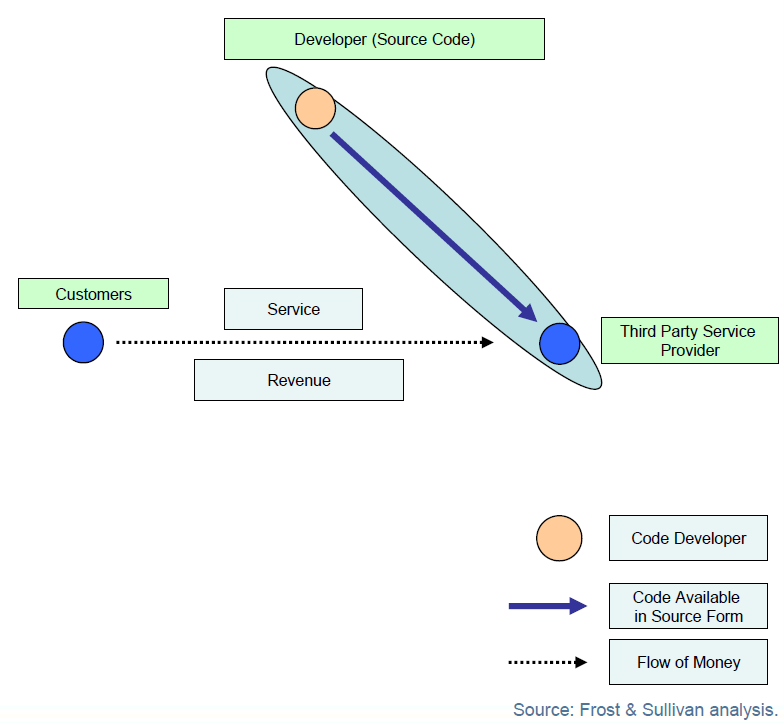
\includegraphics[width=.94\textwidth]{Impact-img2.png}}
%  \caption{The Third-Party Services Model}\label{fig:tps-model}
% \end{figure}

% \begin{compactenum}
% \item The \textbf{GPL model} (see Figure~\ref{fig:gpl-model}): With this model, the vendor
%   is required to make the new code available in source form but it can choose to keep the
%   new code as proprietary and charge for that proprietary software.  The vendor can
%   provide the code commercially as part of a larger platform (hardware/software product)
%   for which the companies receives revenue (license fee for the code + fees for technical
%   support, updates and upgrades).
% \item The \textbf{Third Party Service Model} (see Figure~\ref{fig:tps-model}) Many users
%   may be willing to employ a third party service for distribution, modifications
%   (debugging) and other support.
% \end{compactenum}

\eucommentary{
Where relevant, include information on how the participants will manage
the research data generated and/or collected during the project, in
particular addressing the following issues: What types of data will the
project generate/-collect? What standards will be used? How will this
data be exploited and/or shared/made accessible for verification and
re-use (If data cannot be made available, explain why)? How will this
data be curated and preserved?}

\TOWRITE{E.S. – Nicolas}{, ici je ne peux pas  écrire à ta place. Il faut juste que
tu répondes précisément aux questions posées ci-dessus.}

%Open source software.
%
%
%All software used and/or generated by the project will be Open Source.
%This is a deliberate choice of the project consortium, as commercial
%licenses (and patents) on this type of software only creates barriers
%in our scientific domain.
%
%Benefits of Open Source:
%
%Acquisition and Costs: lower costs, easy access to the infrastructure,
%lower risks of proprietary lock-in
%
%Flexibility: picking up from Open Source projects, reduces dependence on
%supplier, ability to view and modify the source code. Allows peer
%reviewed modifications, community discussions. Open Source provides the
%customer/end user the opportunity to innovate
%
%Support: from developer community.
%
%Besides being cost effective, Open Source software fosters
%reuse, reliability, flexibility, and interoperability.
%
%A consortium agreement will be established to manage ownership and
%access to key knowledge, including software generated by the project.

{\bf Open access policy and data protection.} OpenDreamKit will participate in the Open Research Data Pilot and is fully committed to ensure the open access of relevant project results and data. The consortium will comply with the Guidelines on Open Access to Scientific Publications and Research Data in Horizon 2020. 

The ambitious and interdisciplinary objectives of the project will result in the production of vast amount of research data (we refer to Figure \ref{fig:thebigpicture} and the corresponding subsection for more details). The primary results of the project are expected to take the form of an open-source software, which will be available through the project website and publicly available repositories. Moreover, as the project strives towards efficient integration and representation of various research data and reproducibility of the research results, which represents naturally a challenge, the project will generate a detailed description of the data sources with specifics pertaining to data management (metadata standards, policies for access and sharing and for reuse and distribution, plans for archival and preservation, with accompanying deadlines). This information will be presented in the Data Management Plan, to be delivered within the first six months after the project start and subsequently updated throughout. 

All scientific publications produced in the framework of the project will be either published in open access journals or self-archived using research data repositories. In addition, we will make all experimental data needed to reproduce/validate the results from scientific publications available through research data repositories (e.g. ZENODO, OpenAIRE). 

{\bf Intellectual Property Rights Management.} IPR management will be described in detail in the Consortium Agreement (CA), which will describe all issues regarding the IPR, confidentiality, know-how, rights on exploitation, the rights and obligations of the each partner. The CA will be prepared by the Coordinator, and then signed by all partners before the start of the project. 

Access rights to foreground and background needed for the execution of the project shall be deemed granted, on a royalty-free basis, as of the date of the grant agreement entering into force. Methodology, documents, know-how, software, and tools will be available to all in order to achieve the project objectives during the project lifetime. 

Most of the project results will have joint ownership due to a highly collaborative nature of the project. The CA will specify the terms of the resulting joint ownership, i.e., assignment of shares between joint owners, conditions of use, exploitation and management of jointly used IP. 

The CA will also outline rules for publication procedures to ensure that IP can be protected while minimising publication delay.

The costs related to IPR (including those related to protecting results) and dissemination (i.e., 'gold' open access publications) are included in the project budget of each participating organisation. 

\subsubsection{Communication Activities}
\label{subsubsect:communication}

\eucommentary{Describe the proposed communication measures for promoting the
project and its findings during the period of the grant. Where appropriate
these measures should include social media and public events with user
participation. Measures should be proportionate to the scale of the project,
with clear objectives. They should be tailored to the needs of various audiences,
including groups beyond the project's own community. Where relevant, include
measures for public/societal engagement on issues related to the project.}

Our intention is to increase the attractiveness of mathematics among young generation and females in particular as well as to improve the impact and maximise the visibility of the project activities on the entire VRE ecosystem. The following strategic access points will be used to maximise visibility:

\begin{compactenum}
\item An online presence that explains the OpenDreamKit concept and its applicability in layman's terms and offers significant information (website, social networks, Youtube, press releases).
\item Collaboration with other relevant European and national projects (existing and new ones). We refer to Section \ref{linked-projects} for more details on the linked research and innovation activities.  Presentation of the project results on the annual event 'Worldwide meetings of the free software.' 
\item Collaboration with European and national mathematical societies, e.g., European Mathematical Society, European Women in Mathematics.
\item Presentations/demonstrations at partner institution-specific, locally organised 'science holiday' and 'days of science'.
\item Popularisation papers and communication events addressed to people interested by ICT. 
\item Involvement in workshops / conferences on e-infrastructures and broad mathematical topics, e.g., Swiss Numerical Analysis Day.
\end{compactenum}
%%% Local Variables:
%%% mode: latex
%%% TeX-master: "proposal"
%%% End:

%  LocalWords:  eucommentary programme subsubsection tablehead longtable hline sur est
%  LocalWords:  e-infrastracture sémantique données amont j'ai mal si répond vraiment ce
%  LocalWords:  critère Systeme flushleft arraybslash Ergonomie il faut réflechir façon
%  LocalWords:  rendre l'outil attractif jeune génération génération des chercheurs va je
%  LocalWords:  définir donc terme Réfléchis possibilité tablettes mais aussi l'enseigner
%  LocalWords:  intéressante textgreater partie suivante demande elle ne serait mieux que
%  LocalWords:  unauthorised Maximise subsubsect organisational Pycon IPython Economie tu
%  LocalWords:  Standartisation Logiciel Libre includegraphics Impact-img1.png peux emph
%  LocalWords:  Impact-img2.png écrire répondes précisément posées ci-dessus TOWRITE fbox
%  LocalWords:  Simula Valeriya textwidth textwidth textbf compactenum longtable Jupyter
%  LocalWords:  organisation organise neighbouring Standartization programmes gpl-model
%  LocalWords:  tps-model thebigpicture Popularisation virtualised organisations Logilab
%  LocalWords:  organisations summarise organising capitalise realising minimising
%  LocalWords:  organised


\clearpage

% ---------------------------------------------------------------------------
%  Section 3: Implementation
% ---------------------------------------------------------------------------

\section{Implementation}
\COMMENT{Typical granularity: 5-8 work packages with 3-5 tasks and one
  deliverable per task; 10 milestones}

\subsection{Work Plan --- Work packages, deliverables and milestones}
\label{sect:workplan}
\begin{todo}{from the proposal template}
\begin{enumerate}
\item Describe the overall strategy of the work plan\ednote{Maximum length – one page}
\item Show the timing of the different WPs and their components (Gantt chart or similar).
\end{enumerate}
\end{todo}
\begin{figure}
  \caption{Work package dependencies}
  \label{fig:wp-deps}
\end{figure}

\ganttchart[draft,xscale=.45] 

%%% Local Variables: 
%%% mode: LaTeX
%%% TeX-master: "propB"
%%% End: 

% LocalWords:  workplan.tex ednote wp-deps ganttchart xscale

\newpage

\subsection{Management Structure and Procedures}
\TOWRITE{ALL}{Proofread 3.3 pass 2}
\label{sect:mgt}

\subsubsection{Management}

The project will be coordinated by the Université Paris-Sud (\site{PS}),
represented by Prof.~Nicolas M. Thiéry (Project Coordinator), who has
experience in successfully managing several research projects on the
main \TheProject topics.  A pioneer in community-developed open source
software for research in this field, Thiery founded in 2000 the
Sage-Combinat software project involving 50 researchers in Europe and
abroad.  This project has grown under his leadership to be one of the
largest organised communities of \Sage developers.

The Project Coordinator will be assisted by a part-time (50\%) Project
Manager, who will be hired for this project and located in the
European Affairs and Technology Transfer Office (SAIC) of \site{PS}.
Additional feedback and expertise will be brought by Financial, Legal
and European affairs officers from SAIC.

\subsubsection{Organisational structure and decision-making}

\TOWRITE{Ideally the figure should show that the commission only
  interacts with the Project Coordinator}

\begin{figure}
  \centering
  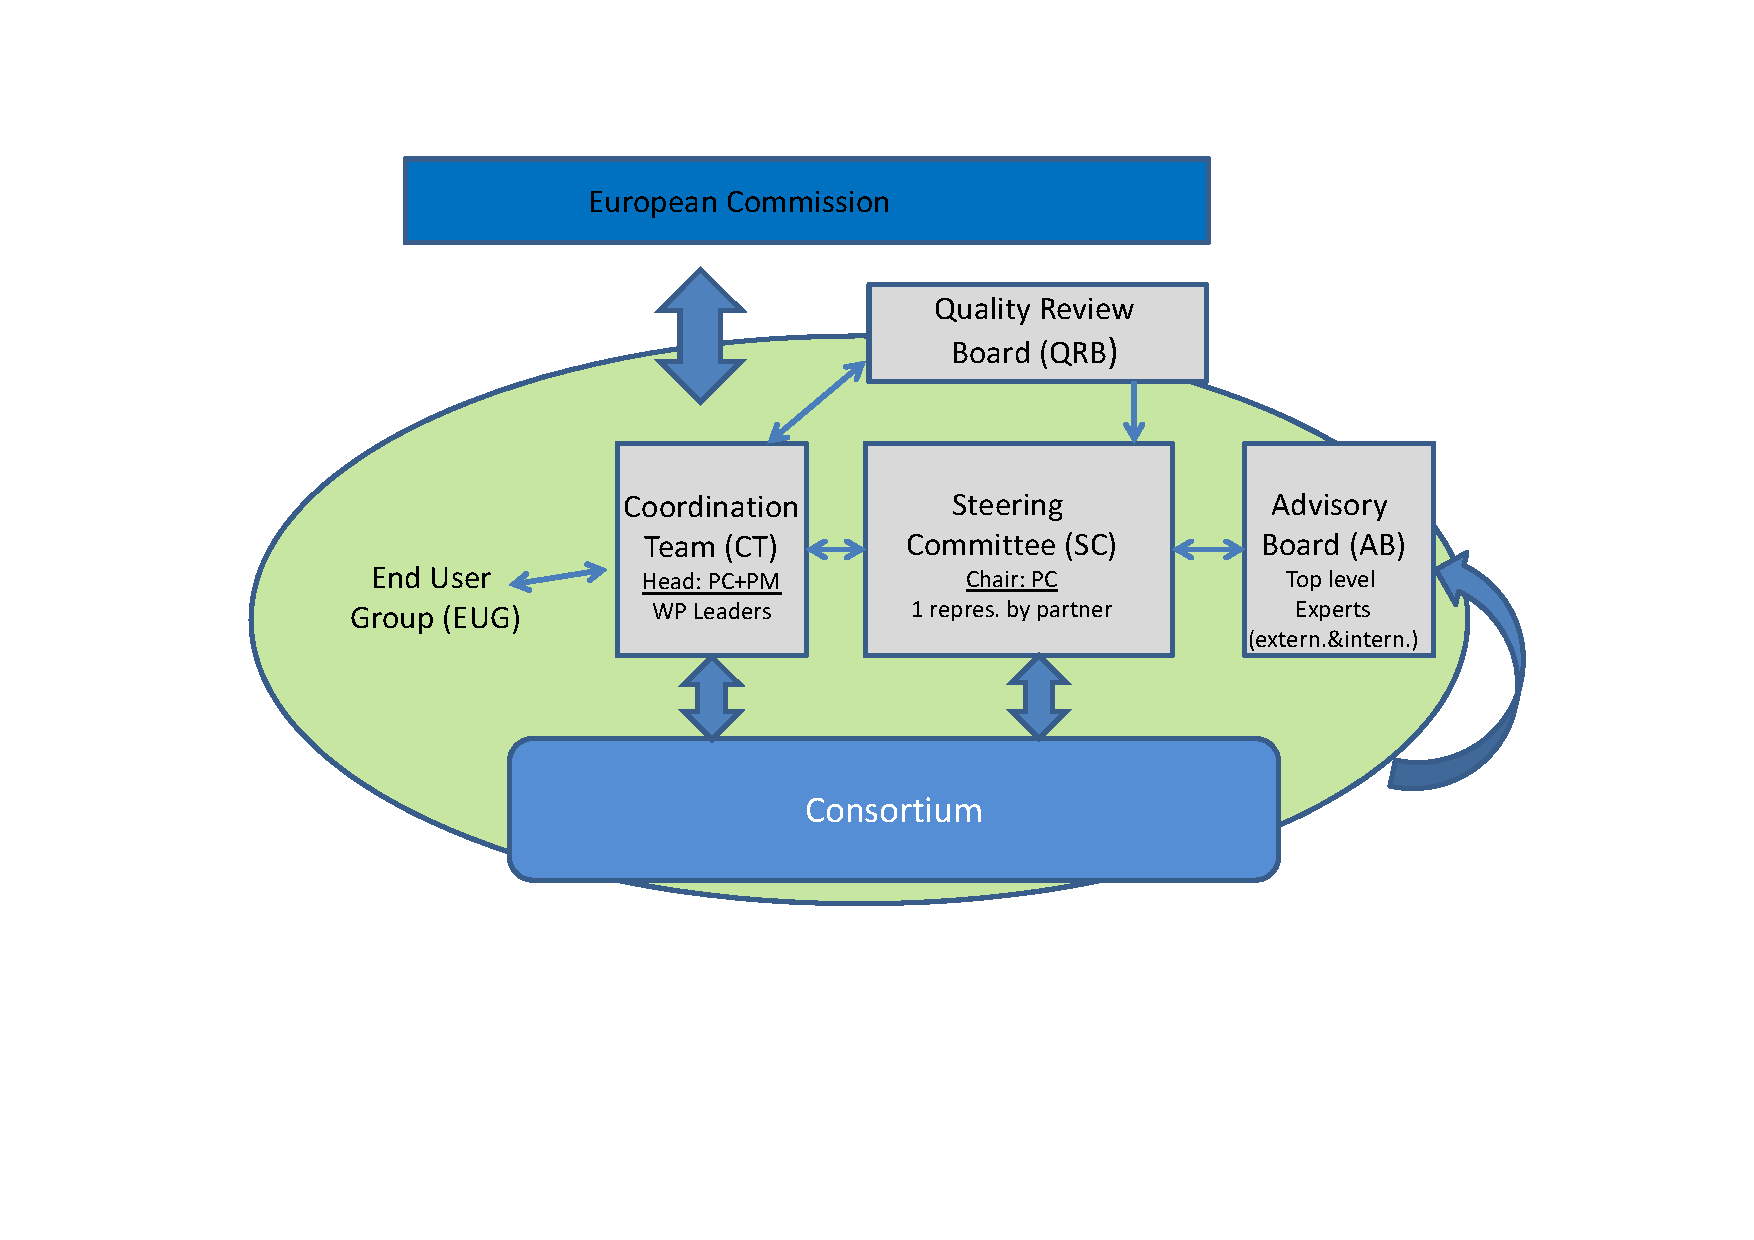
\includegraphics[width=0.75\textwidth]{management_structure.pdf}
  \caption{Management structure}
  \label{figure.management}
\end{figure}

The organisational structure, shown in the Figure~\ref{figure.management}, has been designed
to enable efficient coordination of the project --- the
development and evaluation of a VRE toolkit
integrating several previously separated tools and software and
involving both academic actors and industrial stakeholders.

We have designed the management structure and procedures to deal in a
flexible manner with the following challenges:

\begin{compactitem}
\item to integrate all consortium members and to mobilise their
  expertise, knowledge and networks at every stage of the project;
\item to give the maximum attention to the end-users needs and
  requirements;
\item to continuously involve expertise and knowledge of relevant
  stakeholders and their networks, and
\item to efficiently coordinate the project implementation in a
  collaborative environment and ensure its sustainability.
\end{compactitem}

The coordinator acts as an intermediary between the Partners and
the European Commission. The coordinator will oversee the project
planning, monitor that execution is carried out in time and that
the objectives are achieved and closely interact with the project
officer for project monitoring and delivery of the performance
indicators.  The Project Manager will ensure  efficient day-to-day
management of the project, reporting, feedback to partners on
administrative, financial and legal issues, tracking of  resource
allocation and consumption, and communication inside and outside the
consortium.

The resources of all partners will be mobilised by decentralisation of
responsibilities through the assignment of leadership for work
packages. Clear distribution of tasks, efficient decision making
mechanisms and a sound financial management will safeguard the
achievement of the project's objectives.

\ifgrantagreement\else
\subsubsection{Milestones}
For a description of the milestones and their motivations see
Section~\ref{sec:milestones}; a tabulation of the milestones, which work packages
are involved, and a means of verification can be seen in Table~\ref{tab:milestonetable}.

\milestonetable
\fi

\subsubsection{Project roles}

The following bodies will form the organisational structure of the
\TheProject project : Coordination Team (MT), Steering Committee (SC),
Advisory Board (AB), End User Group (EUG) and Quality Review board
(QRB).

\TOWRITE{NT}{Make this a description}

\begin{description}
\item{\textbf{Coordination Team (CT)}} \nobreak\par
\textbf{Members:} The CT is composed of the Work Package leaders
and headed by the Project Coordinator, assisted by the Project
Manager.

\textbf{Responsibilities:} The CT is an executive body in charge of
the project implementation and monitoring.
It takes operational decisions necessary for the smooth execution of
the project.

\textbf{Tasks:}
\begin{compactenum} 
\item Monitoring the timely execution of the tasks and achievement of
  the objectives;
\item Preparation of scientific and financial progress reports;
\item Controlling Work Package progress by assessing it through technical
  reports developed by the partners;
\item Making proposals to the Steering Committee of re-allocation of
  tasks, resources and financial needs for the fulfilment of the work
  plan;
\item Preparing the drafts and validating the project deliverables to
  be submitted to the Commission; 
\end{compactenum} 

\textbf{Meetings:} Project Coordinator and
  Project Manager can meet any time and at least twice a week. They
  will meet Work-Package leaders every 6 months. If necessary,
  extra meetings will be arranged.



\item{\textbf{Steering Committee (SC)}}\nobreak\par

\textbf{Members:} The SC is chaired by the Project Coordinator
and includes one representative from each partner organisation.

\textbf{Responsibilities:} The SC is the decision-making body in
charge of the strategic orientation of the project.  It takes decisions on scientific
directions, re-allocation of resources, consortium
changes and intellectual property rights.

\textbf{Meetings:} Every 6 months. If necessary, extra-meetings
will be arranged.  Written minutes of each meeting will be produced,
which shall be the formal record of all decisions taken. A procedure
for comment and acceptance is proposed.

\textbf{Voting procedure:} The SC shall not deliberate until all
Members are present or represented.  Each Member shall have one
vote. The SC will work on consensual decisions as much as possible and
resort to voting only if unavoidable. Voting decisions shall be taken
by a majority of two-thirds (2/3) of votes.



\item{\textbf{Advisory board (AB)}}\nobreak\par

\textbf{Members:} top level experts from partner and external
organisations, including both experts from the project scientific
area, and experts on legal and social matters. The following external
persons have already confirmed their interest: William
Stein\footnote{\url{wstein.org}}, lead developer of \SMC, one
representative of the Open Source Software Working Group\footnote{\url{http://www.systematic-paris-region.org/en/get-info-topics/free-and-open-source-software}}
of the Systematic Paris Region Systems \& ICT Cluster,
and Istvan Csabai\footnote{\url{http://complex.elte.hu/~csabai/}} of the
Wigner Research Centre for Physics (WRCP) of the Hungarian Academy of
Sciences.

\textbf{Responsibilities:} to give an independent opinion on
scientific and innovation matters, in order to guaranty quality
implementation of the project, efficient innovation management and
project sustainability.  

\textbf{Meetings:} at the request of the Steering Committee.


\item{\textbf{Quality Review Board (QRB)}}\nobreak\par
\textbf{Members:} The QRB will be composed of 2 senior
researchers from the Consortium, 2 representatives of the End User
Group and 2 experts from the Advisory Board. It will be chaired by one
of the professors within the Consortium. All members will be appointed
at the kick-off meeting of the project.  

\textbf{Responsibilities:}
to monitor the quality of the Deliverables, their whole ‘production
process’ and to recommend improvements during the project to the SC.

\textbf{Meetings:} before publications and reports of the
project.

\item{\textbf{End User Group (EUG)}}\nobreak\par

\textbf{Members:} end-users of the VRE, internal and external to
the consortium, from different disciplines and both from academic and
industrial sector. They are actively involved into the project
execution, and work in close interaction with the project coordinator.

\textbf{Responsibilities:} the EUG is the main actor of the innovation
management within the consortium, as they have a deep understanding of
both market and technical problems, and awareness of
opportunities. The EUG also plays a main role in ensuring the VRE
sustainability.  

\textbf{Tasks:} to control the project execution from the
point of view of the end user needs and requirements, to test the tool
and to detect its potential shortcomings at the early stages, to
propose adaptation measures.  

\textbf{Meetings:} the EUG will have regular
virtual meetings, and will meet physically at least once a year.


\end{description}

\subsubsection{Project management tools and procedures}

Project partners and management bodies will communicate through
a dedicated project web platform, maintained by the Project
Manager. WP leaders will monitor progress of
participants of their WP at least monthly, and participants will inform their WP
leaders when problems are encountered. Major problems will be
discussed in (teleconference) meetings with the Project Coordinator
and Project Manager. Each WP leader will be free to organise
extra meetings with WP partners, if necessary. Scientific and
financial progress reports will be collected, assembled and
transmitted to the Project Coordinator by the WP leaders through the
web platform. On basis of the Progress Reports, the Coordination Team
will monitor progress of the project, identify bottlenecks and find
solutions for these problems. Where needed, adaptations to the project
plan will be made, with the aim of ensuring the delivery of the project
results as agreed with the EC. Major adaptations need to be approved
by the Steering Committee.  If necessary, the SC can submit reports to
the QRB for opinion.

Finally, the EUG, working in close cooperation with the
Project Coordinator, will ensure efficient innovation
management. They will carefully monitor new opportunities in
order to give, if necessary, new directions to the project. For
legal aspects, they will have a feedback from legal officers from the
Coordinator’s European Affairs and Technology Transfer office (SAIC),
specialised in Intellectual Property.

Our management structure and procedures will ensure that our network
of 15 partners from both academic and industrial sectors is focused at
achieving the promised deliverables, efficiently managing the
innovation process and largely opening the VRE to its final users. The
15 partners will sign a Consortium Agreement, in which operational
rules and decision making procedures will be laid down.

\subsubsection{Risk management}\label{sec:risks}

The risk in the project execution as planned is carefully assessed and
managed. We base our plans on long standing experience, and we bring
together the world's experts in the relevant tools and techniques.

A key feature of this project is the involvement of a wide set of
partners from multiple domains. While this ensures complementary
coverage of a wide set of skills and provides robustness in different
ways, we will have to ensure that all partners work as closely knit
team. 

Our open source approach means that all our code and outputs
are open and visible to anybody at sites like Github and bitbucket
throughout the project. In particular, it is common for users of
computational software to use the leading edge versions, thus
beta-testing code in-between major releases. This results in risk
reduction: where our design decision or technical approaches are
controversial, this will be detected early by those users, giving the
consortium useful feedback to consider.

The project coordinator will, with support from the Coordination Team
and Quality Review Board, create a Risk Management Plan
\delivref{management}{ipr} as part of the Management Work Package,
which will be reviewed annually.
\ifgrantagreement\else
An initial risk assessment appears as figure \ref{risk-table}.

\begin{figure}
\begin{center}
\begin{tabular}{|m{.2\textwidth}|m{.12\textwidth}|m{.58\textwidth}|}\hline
  Risk & Level with/without mitigation & Mitigation measures\\\hline

  Recruitment of highly qualified staff & High/Medium &
  Great care was taken identifying pool of candidates to hire from,
  and coordinating with currently running projects to rehire personnel
  with strong track record. Typically, we will rehire European
  postdocs that are currently funded by the Sloan grant to work on
  Jupyter in California and wish to come back to Europe.\\\hline

  Different groups not forming effective team & Medium/Low & Long
  track record of working collaboratively on code across multiple
  sites; Aggressive planning of project meetings, work-shops and
  one-to-one partner visits to facilitate most effective teamwork,
  combining face-to-face time at one site with remote
  collaboration.\\\hline 
  % this also justifies our generous travel budget.

  Implementing infrastructure that does not match the needs of end users & High/Low &
  Most of the members of the consortium are themselves end-users with
  a diverse range of needs and points of views; hence the design of
  the proposal and the governance of the project is naturally steered
  by demand; besides, because we provide a toolkit, users have the
  flexibility to adapt the infrastructure to their needs.\\\hline

  Lack of predictability for tasks that are pursued jointly with
  the community & Medium/Low &
  The PI's have a strong experience managing community-developed
  projects where the execution of tasks depends on the availability of
  partners. Some tasks may end up requiring more manpower from
  \TheProject to be completed on time, while others may be entirely
  taken care of by the community. Reallocating tasks and redefining
  work plans is common practice needed to cater for a
  fast evolving context. Such random factors will be averaged out over
  the large number of independent tasks.\\\hline

  Reliance on external software components & Medium/Low & The non trivial
  software components \TheProject relies on are open source. Most are
  very mature
  and supported by an active community, which offers strong long run
  guarantees.  The critical emerging software component \Jupyter
  builds on \IPython which has been around for a decade and is very
  mature. The other components could be replaced by alternatives, or
  worst comes to worst, taken over by the participants.
  \\\hline
\end{tabular}
\end{center}
\caption{\label{risk-table}Initial Risk Assessment}
\end{figure}
\fi
%\TOWRITE{NT/Eugenia}{Impredictability}

%\includegraphics[width=.94\textwidth]{Pictures/Impact-img1.png}

%   But: since Open Source softwares are freely accessible, security
%   and privacy issues are a concern. Anytime a resource is shared,
%   there is greater risk of unauthorised access and contaminated data.
%   Providers must demonstrate security solutions, which should include
%   physical security controlling access to the facility and protection
%   of user data from corruption and cyber attacks.}


%  LocalWords:  mgt Paris-Sud UPSud Thiery Sage-Combinat decentralisation textwidth hline
%  LocalWords:  textwidth Jupyter slmhnlnhfnhs hsfhs ghshsh includegraphics unauthorised

%%% Local Variables:
%%% mode: latex
%%% TeX-master: "proposal"
%%% End:
%  LocalWords:  TOWRITE subsubsection organisational compactenum ipr Impredictability
%  LocalWords:  textbf nobreak smallbreak


\draftpage
\subsection{Consortium as a Whole}
%\TO WRITE{ALL}{Proofread 3.4 consortium pass 2 [Done by Hans]}
%remove this, as we have more pressing things left.

\eucommentary{\begin{compactitem}
\item
Describe the consortium. How will it match the project's objectives?
How do the members complement one another (and cover the value chain,
where appropriate)? In what way does each of them contribute to the
project? How will they be able to work effectively together?
\item
If applicable, describe the industrial/commercial involvement in the
project to ensure exploitation of the results and explain why this is
consistent with and will help to achieve the specific measures which
are proposed for exploitation of the results of the project (see section 2.3).
\item
Other countries: If one or more of the participants requesting EU funding
is based in a country that is not automatically eligible for such funding
(entities from Member States of the EU, from Associated Countries and
from one of the countries in the exhaustive list included in General
Annex A of the work programme are automatically eligible for EU funding),
 explain why the participation of the entity in question is essential to carrying out the project
\end{compactitem}
}

\TOWRITE{All}{Convert site names to standard abbreviations}

The consortium brings together:
\begin{compactenum}
\item \label{mathsoftware} Lead or core developers of a cross-section of the major open
  source computational components for pure mathematics and applications: \GAP (St.~Andrews,
  Oxford), \Linbox (Grenoble), \MPIR (Kaiserslautern), \Pari (CNRS, Versailles), \Sage
  (Orsay, Versailles, CNRS, Oxford, Warwick, Zürich), \Singular (Kaiserslautern).
\item \label{mathdb} Lead developers of a major online mathematical database: \LMFDB
  (Warwick, Zürich).
\item \label{mathknowledge} Experts in mathematical knowledge management (Bremen).
\item \label{smc} The lead developers of the closest thing currently existing to a Virtual
  Research Environment for mathematics: \SMC (Seattle). Because of the key role of \Sage
  in several aspects of the project, and the relevant experience of \SMC as a forerunner of the types
  of systems we want to build, the informal involvement of this US group is adding great value to our project.
  They are keen to provide the benefit of their experience on an unfunded basis, since they wish to remain closely involved in
  all developments in mathematical VREs.
\item \label{jupyter} Experts and major ``promoters'' of the \Jupyter collaborative user
  interfaces for interactive and exploratory computing in a variety of scientific domains
  (Southampton, Simula, Sheffield, Silesia).
\item \label{pythran} Lead developers of the Pythran system for automatic conversion of
  Python to C++ and experts in numerical code optimisation/parallelisation (\site{LL},
  Grenoble)
\item \label{logilab} A company specialised in open-source based Database and Scientific
  Computing for industry (Logilab); it develops in particular its own virtual environment
  \Simulagora.
\item \label{social} Leading researchers in the sociology of mathematical research and
  collaboration. In particular the coordinating partner of the ``Social Machine of
  Mathematics'' project which has been studying how mathematicians collaborate.
\end{compactenum}





There are many existing points of contact between these groups  and
communities, although many of them are also new to one another. This,
together with the fact that each community is internally collaborative
and part of the broader free software community gives us confidence in
their ability to work together.

\TOWRITE{ALL}{Long track record of collaborations between many of the
  sites. Some of the language below can be used.

Writing interfaces between computer algebra systems from different areas and collaborative
software development are important themes within the DFG Priority Project SPP1489.
As in the {\sc{Sage}} community, networking measures include the regular exchange
of developers and the regular organisation of software workshops (coding sprints) which
bring whole teams together for solution finding and intense code writing. Particular tight
collaborations exist between the {\sc{GAP}} and the {\sc{Singular}} communities, with
major {\sc{GAP-Singular}} developers meetings taking alternately place at St~Andrews,
Kaiserslautern, and Aachen. See \url{http://www.computeralgebra.de/}.
}

The exact role of each partner in each work package is defined
in \ref{sec:workpackages}, but in general terms:
\begin{compactitem}
\item Groups \ref{mathsoftware}, \ref{mathdb}, and
\ref{mathknowledge} (from the list above) will collaborate to design the \TheProject VRE
architecture -- the set of interfaces and standards that allow
components to be assembled into bespoke VREs for particular projects
or areas. This architecture will be informed  by the
experience of \ref{logilab} and \ref{smc}; by the sociological
understanding of \ref{social} and from a
\textbf{diverse range of real world use cases from all areas of scientific
  computing, in academia and industry} drawn from their own user bases
and contributed by \ref{logilab} and \ref{smc}.

They will be supported in this work by \ref{smc}, \ref{jupyter} and \ref{pythran} which
bring respectively expertise in the key technologies \SMC and \Jupyter and the Cython
technology.

\item All the participants will make use of the \TheProject VRE, providing feedback to the
  developers and contributing later to the development of demonstrator projects
  (Objective~\ref{objective:demo}). They will also all participate actively in
  dissemination (Objective~\ref{objective:disseminate}) activities.

\item Group \ref{jupyter} will host and mentor core \Jupyter developers to improve this
  key technology (Objective~\ref{objectives:core}), while \ref{mathsoftware},
  \ref{mathdb}, and \ref{mathknowledge} will update their mathematical software components
  (Objective~\ref{objective:updates}) to comply with the newly developed
  interfaces. \ref{pythran} will be a key asset for this work, providing expertise in
  massive parallelism and HPC, bringing in and further developing the specific \Pythran
  optimisation technology and providing expertise for development of related technologies
  in other components.  Throughout the consortium, groups have substantial
  experience in open source code development.

\item Group \ref{logilab} will further bring in expertise in semantic databases,
  distribution of large software, and open source based business models.

\item Groups \ref{mathsoftware}, \ref{smc}, and \ref{jupyter} already
  have strong experience in community building and engagement
  (Objective~\ref{objective:community}) for instance through the very
  active user and developer communities around \GAP and \Sage. These
  communities and the dissemination to them of the availability new
  free software constitute the primary exploitation route for this
  project. 
\end{compactitem}

Beneficiaries Jacobsuni,USFD, SOUTHAMPTON and UZH are terminated.
\TOWRITE{ALL}{Add previous collaborations}

% joint software/database development
\jointsoft{PS,UB,UO,UV,UW,ZH,UJF,SA,UK,UG} % Sage development
\jointsoft{UO,SA,UK} % GAP development
\jointsoft{UB,UW,UG} % PARI development
\jointsoft{SR,USH,USO,UG,XFEL} % IPython; a bit weak
%\jointsoft{SR,USH,XFEL,UG} % IPython; a bit weak # USO->XFEL
\jointsoft{PS,LL,UW,ZH} % meeting

%joint projects
\jointproj{SA,UK} % IAA GAP5 project
\jointproj{SA,UW,UO} % Science project (CoDiMa)
\jointproj{SR,US} % Education project
\jointproj{USO,UO,XFEL} % eScience project
%\jointproj{XFEL,UO} % eScience project # USO->XFEL
\jointproj{UW,UB,ZH,UK} % LMFDB

%joint supervision
\jointsup{UK,JU,FAU} % Volker Sorge

%joint organization
\jointorga{SA,JU,FAU} % CALCULEMUS WS
\jointorga{SA,UJF} % PASCO'15
\jointorga{JU,ZH,FAU} % CICM
\jointorga{SA,UK} % GAP Days
\jointorga{SA,JU,FAU} % Steve and Mikael, OpenMath events in the 90s
% joint publications
\jointpub{SA,UO} % Steve and Ursula
\jointpub{SA,UK} % Steve and Reimer
\coherencetable[swsites]

%copied pasted JU to FAU and USO to XFEL
%%% Local Variables:
%%% mode: latex
%%% TeX-master: "proposal"
%%% End:

%%% Local Variables:
%%% mode: latex
%%% TeX-master: "proposal"
%%% End:


\draftpage

\subsection{Resources to be Committed}\label{sec:resources}
\TOWRITE{ALL}{Proofread 3.4 pass 2 (especially first paragraph Staff efforts)}

\eucommentary{Please provide the following:
\begin{compactitem}
\item
a table showing number of person/months required (table 3.4a)
\item
a table showing 'other direct costs' (table 3.4b) for participants where
those costs exceed 15\% of the personnel costs (according to the budget
table in section 3 of the administrative proposal forms)
\end{compactitem}}

\subsubsection{Management Level Description of Resources and Budget}
\label{sect:budget-details}

\paragraph{Staff efforts}

\eucommentary{Please indicate the number of person/months over the whole
duration of the planned work, for each work package, for each participant.
Identify the work-package leader for each WP by showing the relevant
person-month figure in bold.}

By design \TheProject is attacking upfront the diverse needs of a
very large community: pure maths and applications. Thanks to its
toolkit approach, it will impact users in many areas of science. This
is a major long term investment which requires the extensive expertise
of a large consortium and the improvement of a great number of
software components. The complex technical nature of the project,
combined with the high quality requirements for guaranteeing long term
sustainability, necessitates recruiting highly experienced software
engineers to complement the participants. Much emphasis is put as well
on studying the social aspects and implementing many demonstrators to
illustrate the breath and depth of potential applications.

This all explains the considerable staff efforts%
\ifgrantagreement.\else{} %
displayed in the following table.
\wpfig[label=fig:staffeffort,caption=Summary of Staff Efforts]
\fi

\paragraph{Travel, dissemination, and outreach}

The community-building nature of this grant proposal requires a large
number of staff exchanges, workshops with project partners, as well as
workshops engaging the wider community in addition to the usual
management and project review meetings. For dissemination, we need to
target the computer science and computational science-focused
communities and their conferences, as well as the domains benefitting
from \TheProject, such as Mathematics and Physical Sciences.

\subparagraph{Guidelines for travel and dissemination}
\label{sect:budget-details-travel}

We use the following guidelines for expected travel expenses:
\euro{2200} for attendance of a typical one week international
conference outside Europe (including travel, subsistence,
accommodation and registration), \euro{1200} for a corresponding
conference in Europe, \euro{750} for a one-week visit of a  project
partner, for instance for coding sprints and one-to-one 
research visits. We expect a similar cost per week while hosting
visitors. For the half-yearly project meetings, we expect on average a
cost of \euro{400} for travel, accommodation and subsistence.

For a partner site with one investigator and one full time researcher,
we expect that both will attend all of the 9 project meetings that take
place every 6 months (cost of 9 * 2 * 400 =
\euro{7200}), and that the site spends \euro{2000} per year to host
external visitors contributing to the project (total \euro{8000}). We
expect the investigator and the researcher in total to do 4 one-week visits
to other sites (each at \euro{750}) every year, totaling \euro{12000} over 4 years).

% 9*2*400 + 2000*4 + 4*750*4
For dissemination, we expect the researcher to attend on average 1
international conference and 2 European meetings per year (totals
\euro{18400}) and the investigator to attend one international and one
european gathering (totals \euro{13600}).
% (2*2200 + 3*1200)*4

Where there are multiple investigators per site, they will share the
travel and associated costs outlined above. Where there are multiple
researchers, or researchers not employed for the full 48 months, the
travel budget is reduced accordingly.

\subparagraph{Guidelines for outreach costs}
\label{sect:budget-outreach-publication-charges}
We also request \euro{1000} per year per partner (several partners
have other means do pay these costs, and for them these are not needed) 
to pay for open access publication charges.

\label{sect:budget-outreach-workshops}
We request funds for outreach activities such as workshops that
facilitate community building, disseminate best practice and
encourages sustained contributions of the community to the project and
beyond the lifetime of the funding. For  a one-week workshop reaching
out to the community, we cost these at about 400 EUR per participant
to provide accommodation and catering. A workshop for 15 people will
thus cost about \euro{6000}. Participants donate their time and will fund
their own travel. The particular budgeted cost will depend on the
local availability of accommodation and will thus vary from workshop to
workshop. We use creative means to increase value and improve
community building where possible, for example by cooking food
ourselves as done in this recent workshop
\href{http://wiki.sagemath.org/days57}{http://wiki.sagemath.org/days57}.

Details are given in the tables below and in the work packages.

\bigskip

\subsubsection{Resource summaries for consortium member sites}
\label{resources.summary}

%%%%%%%%%%%%%%%%%%%%%%%%%%%%%%%%%%%%%%%%%%%%%%%%%%%%%%%%%%%%%%%%
%
% Guidelines for completion of partner specific resource summary:
%
%
% Please explain how many person months for each person are
% requested. Say who is the local lead. Say anything that helps to
% understand why people are recruited as you plan, in particular if
% this deviates from having one research for 48 months.  We can also
% use this bit of the proposal (and the table, see below) to address
% any other unusual arrangements.
%
%
% The table should contain all non-staff costs (the EU requests that
% this table must be present if the non-staff costs exceed
% 15% of the total cost, but it is good practice and will show
% openness and transparency that we show the data for all partners).
%
% Link back from the table to the work packages and tasks for which
% the expenses are required. Add information that makes it easier to
% understand why the expenses are justified.
%
%     To refer to a task in a work package, use "\taskref{WP-ID}{TASK-ID}" where
%     WP-ID is the ID of the work package:
%        WP#: WP-ID - full title
%        ----------------------
%        WP1: 'management' - Management
%        WP2: 'community' - Community Building and Engagement
%        WP3: 'component-architecture' - Component Architecture
%        WP4: 'UI' - User interfaces
%        WP5: 'hpc' - High Performance Computing
%        WP6: 'dksbases' - Data/Knowledge/Software-Bases
%        WP7: 'social-aspects' - Social Aspects
%        WP8: 'dissem' - Dissemination
%
%
%     and "TASK-ID" is the ID of the task. You can set this using
%
%       \begin{task}[id=TASK-ID,title=Math Search Engine,lead=JU,PM=10,lead=JU]
%
%     To refer to deliverables, use "\delivref{WP-ID}{DELIV-ID}" where DELIV-ID is
%     the ID of the deliverable that can be set like this:
%
%       \begin{wpdeliv}[due=36,id=DELIV-ID,dissem=PU,nature=DEM]
%           {Exploratory support for semantic-aware interactive widgets providing views on objects
%           represented and or in databases}
%       \end{wpdeliv}
%
%
% The table is pre-populated with entries most sites are likely
% to need. If a line does not apply to you, just delete it. If you need
% an extra line, then add it. Use common sense: the number of rows should not
% be very big, but at the same time it is useful to give some breakdown/explanation
% of costs.
%
%
% Eventually, try to create you entry similar in style to the others.
% (The Southampton entry is fully populated, so use this as guidance
% if in doubt.)
%
%
%%%%%%%%%%%%%%%%%%%%%%%%%%%%%%%%%%%%%%%%%%%%%%%%%%%%%%%%%%%%%%%%

In this section we briefly describe the requested resources. See the
participant descriptions in the description of the consortium for the
specific role of each member.

%%%%%%%%%%%%%%%%%%%%%%%%%%%%%%%%%%%%%%%%%%%%%%%%%%%%%%%%%%%%%%%%%%%%%%%%%%%%%%
\paragraph{Resources Université Paris-Sud}

\site{PS} requests 12 person months for the project coordinator
(Nicolas M. Thiéry), 5 person months for two researchers (Florent
Hivert, and Samuel Lelièvre) and for the lead PI (Viviane Pons), 44 person-months for a full time developer and 5.5 person-months for a part-time developer, 24 months for a postdoc, and
24 months for a part time project manager for the full duration of the
project.

% 4 * 4k: Developper workshops Cernay
% 6k: Jupyter-Sage
% 2 * 6k: Women in Sage
% Training: 2*4k
% Dissemination CIRM: 16k
% Kickup and final meeting: 2*16k
% workshop: 82k
% (2 * 4 + 3 + 2 * 4 )*(1*2200 + 2*1200) + 2*2000 + 4*750
% travel: 103K


% update table as is appropriate for your contribution. Please remove unused lines.
% Note: it would be nicer to use \site in the caption, but this breaks ...
\bigskip
\begin{table}[H]
\begin{tabular}{|r|r|p{8.5cm}|}
\hline
\textbf{1: \site{PS}} & \textbf{Cost (\euro)} & \textbf{Justification} \\\hline
\textbf{Travel} & 85,139 & Travel (see the guidelines \ref{sect:budget-details-travel})\\\hline
\textbf{Publication charges} & 1,000 & Open access publication charges (see \ref{sect:budget-outreach-publication-charges})\\\hline
%\textbf{Equipment} & ?,??? &  \\\hline    %\taskref{WP-ID}{TASK-ID}
\textbf{Other goods and services} & 92,000 & 8 developer
workshops~\taskref{dissem}{devel-workshops}, 4 training and
dissemination workshops~\taskref{dissem}{dissemination-communication},
audits certificates on the financial statements \\\hline   %\taskref{WP-ID}{TASK-ID} \delivref{WP-ID}{DELIV-ID}
\textbf{Total} & 178,139\\\cline{1-2}
\end{tabular}
\caption{Overview: Non-staff resources to be committed at UPSud (all in \texteuro)}\vspace*{-1em}
\end{table}

%%%%%%%%%%%%%%%%%%%%%%%%%%%%%%%%%%%%%%%%%%%%%%%%%%%%%%%%%%%%%%%%%%%%%%%%%%%%%%
\paragraph{Resources CNRS}

CNRS requests
14 person months for the lead PI Vincent Delecroix,
13 for the \PariGP head Karim Belabas,
8 person months for PIs Adrien Boussicault,
7 person months for PI Bill Allombert,
6 person months for PI S\'ebastien Labb\'e,
5 person months for PI Loïc Gouarin, and
30 person months for a full time developer working on tasks~\taskref{hpc}{hpc-pari},
\taskref{hpc}{hpc-combi}, \taskref{UI}{Sage-display} and \taskref{UI}{pari-python}.

\bigskip
\begin{table}[H]
\begin{tabular}{|r|r|p{8.5cm}|}
\hline
\textbf{2: \site{UB}} & \textbf{Cost (\euro)} & \textbf{Justification} \\\hline
\textbf{Travel}
  &  56,700 & Travel (see the guidelines \ref{sect:budget-details-travel})\\\hline
\textbf{Publication charges}
  &   1,000 & Open access publication charges (see \ref{sect:budget-outreach-publication-charges})\\\hline
%%\textbf{Equipment}
%%  &   0 &  \\\hline    %\taskref{WP-ID}{TASK-ID}
\textbf{Other goods and services}
  & 82,802 &
4 Ateliers \Pari \taskref{dissem}{devel-workshops},
A series of dissemination workshops and trainings in developed and developing countries \taskref{dissem}{dissemination}
 \\\hline   %\taskref{WP-ID}{TASK-ID} \delivref{WP-ID}{DELIV-ID}
\textbf{Total}
 & 140,502\\\cline{1-2}
\end{tabular}
\caption{Overview: Non-staff resources to be committed at CNRS (all in \texteuro)}\vspace*{-1em}
\end{table}


%%%%%%%%%%%%%%%%%%%%%%%%%%%%%%%%%%%%%%%%%%%%%%%%%%%%%%%%%%%%%%%%%%%%%%%%%%%%%%
\paragraph{Resources Jacobs University Bremen
}

\site{JU} requests 6 PM each for a research programmer (Dr. Christian Maeder) and a junior
researcher (Mihnea Iancu M.Sc.). The first will do much of the actually system development
in \WPref{UI} and \WPref{dksbases} while the latter will concentrate on the cases studies
in \WPref{dksbases}. The rest of the PM (11) are to be dispatched within the other \site{JU} participants.

\bigskip
\begin{table}[H]
\begin{tabular}{|r|r|p{8.5cm}|}
  \hline
  \textbf{3: \site{JU}} & \textbf{Cost (\euro)} & \textbf{Justification} \\\hline
  \textbf{Travel} & 8,000 & Travel (see the guidelines \ref{sect:budget-details-travel})\\\hline
  \textbf{Publication charges} & 1,500 & Open access publication charges (see \ref{sect:budget-outreach-publication-charges})\\\hline
  \textbf{Equipment} & & \\\hline
  \textbf{Other goods and services} & & \\\hline
  \textbf{Total} & 9,500\\\cline{1-2}
\end{tabular}
\caption{Overview: Non-staff resources to be committed at JacobsUni (all in \texteuro)}\vspace*{-1em}
\end{table}

%%%%%%%%%%%%%%%%%%%%%%%%%%%%%%%%%%%%%%%%%%%%%%%%%%%%%%%%%%%%%%%%%%%%%%%%%%%%%%
\paragraph{Resources Universit\'{e} Grenoble Alpes}

% See guidance above ("Guidelines for completion of partner specific resource summary") for what to add here.
UGA requests 12 person months for an engineer (Pierrick Brunet) starting in
month 0 and working on \taskref{hpc}{pythran}, 24 person
months for another engineer starting in month 12 and working on \taskref{hpc}{hpc-linbox}, 15 person months for the lead PI
(Clément Pernet) and 9 person months for a PI (Jean-Guillaume Dumas).
The lead PI will take on all management responsibilities. The
engineers will not be employed for the whole project duration, and
the PIs will carry out all tasks for the project in the remaining
period.

% update table as is appropriate for your contribution. Please remove unused lines.
\bigskip
\begin{table}[H]
\begin{tabular}{|r|r|p{8.5cm}|}
\hline
\textbf{4: \site{UJF}} & \textbf{Cost (\euro)} & \textbf{Justification} \\\hline
\textbf{Travel} & 60,850 & Travel (see the guidelines \ref{sect:budget-details-travel})\\\hline
\textbf{Publication charges} & 1,000 & Open access publication charges (see \ref{sect:budget-outreach-publication-charges})\\\hline
\textbf{Equipment} & 24,000 &A large multicore server with
multiple accelerators to experiment heterogeneous computing; 2 laptops  \\\hline     %\taskref{WP-ID}{TASK-ID}

\textbf{Other goods and services} & 34,000 & 2 developer workshops: HPC and Pythran,
audits certificates on the financial statements \\\hline   %\taskref{WP-ID}{TASK-ID} \delivref{WP-ID}{DELIV-ID}
\textbf{Total} & 119,850\\\cline{1-2}
\end{tabular}
\caption{Overview: Non-staff resources to be committed at UGA (all in \texteuro)}\vspace*{-1em}
\end{table}


%%%%%%%%%%%%%%%%%%%%%%%%%%%%%%%%%%%%%%%%%%%%%%%%%%%%%%%%%%%%%%%%%%%%%%%%%%%%%%
\paragraph{Resources University of Kaiserslautern}


% See guidance above ("Guidelines for completion of partner specific resource summary") for what to add here.

\site{UK} requests 48 person months for a researcher to work on
tasks~\taskref{hpc}{hpc-singular} (46 PM), \taskref{UI}{ipython-kernels} (2 PM), 12
person months for a researcher starting in month 6 to work on
\taskref{hpc}{hpc-mpir}. The cost for Professor Decker's
activities within \TheProject (6 PM), including the related overhead,
will be covered by \site{UK} and is therefore not part of the requested
funding. The lead PI will take on all management responsibilities.


% update table as is appropriate for your contribution. Please remove unused lines.
\bigskip
\begin{table}[H]
\begin{tabular}{|r|r|p{8.5cm}|}
\hline
\textbf{5: \site{UK}} & \textbf{Cost (\euro)} & \textbf{Justification} \\\hline
\textbf{Travel} & 67,100 & Travel (see the guidelines \ref{sect:budget-details-travel})\\\hline
\textbf{Other goods and services} & 67,600 &
  5 developer workshops~\taskref{dissem}{devel-workshops},
  audits certificates on the financial statements \\\hline
\textbf{Total} & 134,700\\\cline{1-2}
\end{tabular}
\caption{Overview: Non-staff resources to be committed at UNIKL (all in \texteuro)}\vspace*{-1em}
\end{table}

%%%%%%%%%%%%%%%%%%%%%%%%%%%%%%%%%%%%%%%%%%%%%%%%%%%%%%%%%%%%%%%%%%%%%%%%%%%%%%
\paragraph{Resources University of Oxford}

University of Oxford requests in total 29 Person-Months for its lead PI Dmitrii Pasechnik, Ursula martin and Edith Elkind. 
Martin and Elkind both hold personal fellowships (funded by EPSRC (UK) and by ERC, respectively)
on topics closely related to the project, enabling them to take part 
in the project only at a fraction of the full cost; however, 
they will need funding to travel to project meetings.
Open access publication charges will be met by the host institution.

\bigskip
\begin{table}[H]
\begin{tabular}{|r|r|p{8.5cm}|}
\hline
\textbf{6: \site{UO}} & \textbf{Cost (\euro)} & \textbf{Justification} \\\hline
\textbf{Travel} & 25,000 & Travel (see the guidelines \ref{sect:budget-details-travel})\\\hline
\textbf{Equipment} & 3,000 & Laptop and a large display for a co investigator \\\hline    %\taskref{WP-ID}{TASK-ID}

\textbf{Total} & 28,000\\\cline{1-2}
\end{tabular}
\caption{Overview: Non-staff resources to be committed at UOXF (all in \texteuro)}\vspace*{-1em}
\end{table}

%%%%%%%%%%%%%%%%%%%%%%%%%%%%%%%%%%%%%%%%%%%%%%%%%%%%%%%%%%%%%%%%%%%%%%%%%%%%%%
\paragraph{Resources University of Silesia}

University of Silesia will include three people in the project and
their involvement will 12 person months each. Jerzy Luczka and Jan Aksamit will
work on interactive books \taskref{dissem}{ibook} which will
demonstrate the real case of using both Structured Text and
interactive features of the VRE. Marcin Kostur will lead and
contribute to this task as well.

Marcin Kostur will lead the part of \taskref{UI}{cfd-vis} which will
be connected with 3d visualisation of data produced by the Lattice
Boltzmann software 'sailfish'. After initial research work done
together with Simula (task leader) will require to subcontract the
development of software visualisation.

The justification for subcontracting is as follows. We have much
experience as users of 3d visualisation software for fluid
dynamics. However the expertise in Computer Graphics (e.g. WebGL) is
not enough at the Department of Mathematics, Physics and
Chemistry. Instead of building the expertise it is financially more
efficient to specify and outsource the programming task to professionals.

% travel (4*2200+5*750+5*400)*1.25

\bigskip
\begin{table}[H]
\begin{tabular}{|r|r|p{8.5cm}|}
\hline
\textbf{7: \site{US}} & \textbf{Cost (\euro)} & \textbf{Justification} \\\hline
\textbf{Travel} & 18,188 & Travel (see the guidelines \ref{sect:budget-details-travel})\\\hline
%\textbf{Publication charges} & 0,000 & Open access publication charges (see \ref{sect:budget-outreach-publication-charges})\\\hline
%\textbf{Other goods and services} & 50,000 & Subcontracting costs  \\\hline   %\taskref{WP-ID}{TASK-ID} \delivref{WP-ID}{DELIV-ID}
\textbf{Total} & 18,188\\\cline{1-2}
\end{tabular}
\caption{Overview: Non-staff resources to be committed at USlaski (all in \texteuro)}\vspace*{-1em}
\end{table}

%%%%%%%%%%%%%%%%%%%%%%%%%%%%%%%%%%%%%%%%%%%%%%%%%%%%%%%%%%%%%%%%%%%%%%%%%%%%%%
\paragraph{Resources University of Sheffield}

Sheffield requests 50.03 person months with a main focus on \WPref{dissem} (31.33 PM).
The remaining PM are to be split between \WPref{hpc}, \WPref{UI} and \WPref{management}.
The lead PI will take on all management responsibilities. Two researchers will be employed, one 
with a specific focus on the SGE Implementation \taskref{hpc}{hpc-jupyter}.
The other for a period of whose focus will be on user
interfaces, social aspects \taskref{social-aspects}{social-output} and
course development \taskref{dissem}{project-intro}.  Researchers will
not be employed for the whole project duration, and the PIs will carry
out all tasks for the project in the remaining period.

% See guidance above ("Guidelines for completion of partner specific resource summary") for what to add here.

% Travel costs computation: project meetings + external hosting + site visits + conference travel
% 9*2*400 + 2000*4 + 4*750*2 + (2*2200 + 3*1200)*4

% update table as is appropriate for your contribution. Please remove unused lines.
\bigskip
\begin{table}[H]
\begin{tabular}{|r|r|p{8.5cm}|}
\hline
\textbf{8: \site{USH}} & \textbf{Cost (\euro)} & \textbf{Justification} \\\hline
\textbf{Travel} & 10,000 & Travel (see the guidelines \ref{sect:budget-details-travel})\\\hline
\textbf{Publication charges} & 2,000 & Open access publication charges (see \ref{sect:budget-outreach-publication-charges})\\\hline
\textbf{Equipment} & 5,000 & High performance laptops and multi touch large screen for \taskref{social-aspects}{social-output} \\\hline

\textbf{Other goods and services} & 3,104.55 & Workshops (Project meeting and two dissemination workshops, see \taskref{dissem}{project-intro}),
  HPC Compute Time (see \taskref{hpc}{hpc-jupyter}),
  audits certificates on the financial statements \\\hline
\textbf{Total} & 20 104,55 \\\cline{1-2}
\end{tabular}
\caption{Overview: Non-staff resources to be committed at USFD (all in \texteuro)}\vspace*{-1em}
\end{table}

%%%%%%%%%%%%%%%%%%%%%%%%%%%%%%%%%%%%%%%%%%%%%%%%%%%%%%%%%%%%%%%%%%%%%%%%%%%%%%
% \paragraph{Original Resources Southampton}
%
% Southampton requests 38 person months for a researcher (expected to
% start in month 4 of the project), 6 person months for the lead PI
% (Hans Fangohr) and 2 person months for the co investigator (Ian
% Hawke). The lead PI will take on all management responsibilities. The
% researcher will not be employed for the whole project duration, and
% the PIs will carry out all tasks for the project in the remaining
% period.
%
% \bigskip
% \begin{table}[H]
% \begin{tabular}{|r|r|p{8.5cm}|}
% \hline
% \textbf{9: \site{USO}} & \textbf{Cost (\euro)} & \textbf{Justification} \\\hline
% \textbf{Travel} & 51,500& Travel (see the guidelines \ref{sect:budget-details-travel})\\\hline
% \textbf{Publication charges} & 4,000 & Open access publication charges (see \ref{sect:budget-outreach-publication-charges})\\\hline
% \textbf{Equipment} & 10,000 & HPC Workstation (6k) to host
% micromagnetic VRE web server, \taskref{UI}{oommf-nb-ve}, and two high performance laptops (2x2k)\\\hline
% \textbf{Other goods and services} & 24,800 &
%   4 Dissemination workshops overseas (travel for teachers \& room hire),
%   \taskref{dissem}{dissemination-of-oommf-nb-workshops},
%   audits certificates on the financial statements\\\hline
% \textbf{Total} & 90,300\\\cline{1-2}
% \end{tabular}
% \caption{Overview: Non-staff resources to be committed at SOUTHAMPTON (all in \texteuro)}\label{tab:resources-non-staff-southampton}\vspace*{-1em}
% \end{table}


\paragraph{Resources Southampton}

Southampton requests 16 person months for a researcher and 3 person months for the lead PI
(Hans Fangohr). The lead PI will take on all management responsibilities.

\bigskip
\begin{table}[H]
\begin{tabular}{|r|r|p{8.5cm}|}
\hline
\textbf{9: \site{USO}} & \textbf{Cost (\euro)} & \textbf{Justification} \\\hline
\textbf{Travel} & 15000& Travel (see the guidelines \ref{sect:budget-details-travel})\\\hline
\textbf{Equipment} & 4,000 & two high performance laptops\\\hline
\textbf{Total} & 19,000\\\cline{1-2}
\end{tabular}
\caption{Overview: Non-staff resources to be committed at SOUTHAMPTON (all in \texteuro)}\label{tab:resources-non-staff-southampton}\vspace*{-1em}
\end{table}




%%%%%%%%%%%%%%%%%%%%%%%%%%%%%%%%%%%%%%%%%%%%%%%%%%%%%%%%%%%%%%%%%%%%%%%%%%%%%%
\paragraph{Resources University of St Andrews}

St Andrews requests 9.6 person months for the lead PI
(Steve Linton), 24 person months for the co-investigator
(Alexander Konovalov) and 48 person months for the 
researcher (Markus Pfeiffer). The lead PI will take on all 
management responsibilities.

\bigskip
\begin{table}[H]
\begin{tabular}{|r|r|p{8.5cm}|}
\hline
\textbf{10: \site{SA}} & \textbf{Cost (\euro)} & \textbf{Justification} \\\hline
\textbf{Travel} & 76,800 & Travel (see the guidelines \ref{sect:budget-details-travel})\\\hline
\textbf{Publication charges} & 4,000 & Open access publication charges (see \ref{sect:budget-outreach-publication-charges})\\\hline
\textbf{Equipment} & 15,000 & Compute servers for parallel software development and testing
(tasks \taskref{hpc}{hpc-gap}, \taskref{component-architecture}{component-for-HPC}) \\\hline

\textbf{Other goods and services} & 21,500 &
  2 dissemination workshops (room hire and subsistence for external participants; task \taskref{dissem}{devel-workshops}),
  audits certificates on the financial statements
 \\\hline
\textbf{Total} & 117,300\\\cline{1-2}
\end{tabular}
\caption{Overview: Non-staff resources to be committed at USTAN (all in \texteuro)}\vspace*{-1em}
\end{table}


%%%%%%%%%%%%%%%%%%%%%%%%%%%%%%%%%%%%%%%%%%%%%%%%%%%%%%%%%%%%%%%%%%%%%%%%%%%%%%
\paragraph{Resources Universit\'{e} de Versailles Saint-Quentin}

Universit\'{e} de Versailles Saint-Quentin requests 12 person months
for the lead PI (Luca De Feo) and 2 person months for a researcher
(Nicolas Gama). Because of its small size and geographical proximity
to \site{PS}, Universit\'{e} de Versailles is not going to hire any
full-time personnel for the project.

\bigskip
\begin{table}[H]
\begin{tabular}{|r|r|p{8.5cm}|}
\hline
\textbf{11: \site{UV}} & \textbf{Cost (\euro)} & \textbf{Justification} \\\hline
\textbf{Travel} & 12,600 & Travel (4 EU conferences, 4 one week visits to project partners, 12 project meetings)\\\hline
\textbf{Total} & 12,600\\\cline{1-2}
\end{tabular}
\caption{Overview: Non-staff resources to be committed at UVSQ (all in \texteuro)}\vspace*{-1em}
\end{table}

%%%%%%%%%%%%%%%%%%%%%%%%%%%%%%%%%%%%%%%%%%%%%%%%%%%%%%%%%%%%%%%%%%%%%%%%%%%%%%
\paragraph{Resources University of Warwick}

Warwick requests 24 person months for a researcher expected to start
around month 6 of the project to work on WP6, and 3 person months for
the lead PI (John Cremona) for WP1 (Management) and WP6. The
researcher will not be employed for the whole project duration, and
the PI will carry out any remaining tasks for the project.  The PI,
who is also PI on the LMFDB grant, will be able to use alternative
funding for conference attendance, and only requires travel support
for project meetings and visiting other sites.  The workshop to be
hosted will be joint with the LMFDB project and part-funded by the
LMFDB grant.  Open access publication charges will be met by the host
institution.

% update table as is appropriate for your contribution. Please remove unused lines.
\bigskip
\begin{table}[H]
\begin{tabular}{|r|r|p{8.5cm}|}
\hline
\textbf{12: \site{UW}} & \textbf{Cost (\euro)} & \textbf{Justification} \\\hline
\textbf{Travel} & 9,600 & Project meetings and partner site visits;
investigator co-funded by LMFDB grant (see \ref{sect:budget-details-travel})\\\hline
\textbf{Equipment} & 4,000 & laptops for investigator and researcher\\\hline    %\taskref{WP-ID}{TASK-ID}

\textbf{Other goods and services} & 12,000 & Hosting one workshop
co-funded by LMFDB project\\\hline   %\taskref{WP-ID}{TASK-ID} \delivref{WP-ID}{DELIV-ID}
\textbf{Total} & 25,600\\\cline{1-2}
\end{tabular}
\caption{Overview: Non-staff resources to be committed at UWarwick (all in \texteuro)}\vspace*{-1em}
\end{table}

%%%%%%%%%%%%%%%%%%%%%%%%%%%%%%%%%%%%%%%%%%%%%%%%%%%%%%%%%%%%%%%%%%%%%%%%%%%%%%
\paragraph{Resources University of Z\"{u}rich}
Zurich will employ one person associated with the project, Paul-Olivier Dehaye. Twelve person-months will be dedicated to \WPref{dksbases} and spread over the four years, with an extra one for the management (\WPref{management}). He will devote additional time to these efforts, paid from other sources (University of Zurich and Swiss Science Foundation).

He will lead tasks \taskref{dksbases}{data-assessment}, and assist for
\taskref{dksbases}{data-design}, \taskref{dksbases}{data-triform},
\taskref{dksbases}{data-foundationCAS}, \taskref{dksbases}{data-findstat} and
\taskref{dksbases}{data-LMFDB}. He is in charge of deliverables \delivref{dksbases}{conv},
and \delivref{dksbases}{lfmverif}.

\bigskip
\begin{table}[H]
\begin{tabular}{|r|r|p{8.5cm}|}
\hline
\textbf{13: \site{ZH}} & \textbf{Cost (\euro)} & \textbf{Justification} \\\hline
\textbf{Travel} & 26,800 & Travel (see the guidelines \ref{sect:budget-details-travel})\\\hline
\textbf{Publication charges} & 4,000 & Open access publication charges (see \ref{sect:budget-outreach-publication-charges})\\\hline
\textbf{Equipment} & 2,000 &  laptop for investigator \\\hline    %\taskref{WP-ID}{TASK-ID}

%\textbf{Other goods and services} & ?,??? & Workshops \\\hline   %\taskref{WP-ID}{TASK-ID} \delivref{WP-ID}{DELIV-ID}
\textbf{Total} & 32,800\\\cline{1-2}
\end{tabular}
\caption{Overview: Non-staff resources to be committed at UZH (all in \texteuro)}\vspace*{-1em}
\end{table}


%%%%%%%%%%%%%%%%%%%%%%%%%%%%%%%%%%%%%%%%%%%%%%%%%%%%%%%%%%%%%%%%%%%%%%%%%%%%%%
\paragraph{Resources Logilab}

Logilab requests 36 person months for its engineers (Julien Cristau,
Florent Cayré and Olivier Cayrol). They will bring their expertise
(database design, software architecture, computer-domain knowledge) to
numerous tasks, and will notably contribute to the packaging of \Sage
(\taskref{component-architecture}{mod-packaging}), the enhancement of
existing forges (\taskref{component-architecture}{workflow}) and the
addition of HTML5 widgets in notebooks
(\taskref{UI}{dynamic-inspect}).

Logilab requests 12 person months for subcontracting an engineer
(Serge Guelton), main developer of \Pythran, that will work on
\taskref{hpc}{pythran}.

% Travels: 1 conference extra-EU, 4 conferences EU, 9 project meetings for 2 persons, 4 workshops
% 1*2200 + 4*1200 + 2*2000 + (9*2)*400 + 4*750 = 17,200


\bigskip
\begin{table}[H]
\begin{tabular}{|r|r|p{8.5cm}|}
\hline
\textbf{14: \site{LL}} & \textbf{Cost (\euro)} & \textbf{Justification} \\\hline
\textbf{Travel} & 17,200 & Travel (see the guidelines \ref{sect:budget-details-travel})\\\hline
\textbf{Total} & 17,200\\\cline{1-2}
\end{tabular}
\caption{Overview: Non-staff resources to be committed at Logilab (all in \texteuro)}\vspace*{-1em}
\end{table}

%%%%%%%%%%%%%%%%%%%%%%%%%%%%%%%%%%%%%%%%%%%%%%%%%%%%%%%%%%%%%%%%%%%%%%%%%%%%%%
\paragraph{Simula Research Laboratory}

Simula requests 29 person months for research activities to lead Work package 4 and contribute to its specific tasks.
We also dedicate 4 person months for management  as well as  dissemination and communication activities (to be split equally). These activities will be mainly performed by the lead PI with the extensive support of the local management team.  
% update table as is appropriate for your contribution. Please remove unused lines.
\bigskip
\begin{table}[H]
\begin{tabular}{|r|r|p{8.5cm}|}
\hline
\textbf{15: \site{SR}} & \textbf{Cost (\euro)} & \textbf{Justification} \\\hline
\textbf{Travel} & 56,200 & Travel (see the guidelines \ref{sect:budget-details-travel})\\\hline
\textbf{Publication charges} & 4,000 & Open access publication charges (see \ref{sect:budget-outreach-publication-charges})\\\hline
%\textbf{Equipment} & 0 &  \\\hline    %\taskref{WP-ID}{TASK-ID}

\textbf{Other goods and services} & 11,500 &
   Organisation of the Jupyter workshop,
   audits certificates on the financial statements
   \\\hline   %\taskref{WP-ID}{TASK-ID} \delivref{WP-ID}{DELIV-ID}
\textbf{Total} & 71,700\\\cline{1-2}
\end{tabular}
\caption{Overview: Non-staff resources to be committed at Simula (all in \texteuro)}\vspace*{-1em}
\end{table}

%%%%%%%%%%%%%%%%%%%%%%%%%%%%%%%%%%%%%%%%%%%%%%%%%%%%%%%%%%%%%%%%%%%%%%%%%%%%%%
\paragraph{Resources Ghent University}
Ghent will employ one person associated with the project, Jeroen Demeyer, who is also the PI for UGent. 14 person-months will be dedicated to WP3 and 14 person-months to WP4. He will additionnaly use a 1.5 person-month for WP1 and 1 person-month for WP2. He is in charge of D4.13.


\bigskip
\begin{table}[H]
\begin{tabular}{|r|r|p{8.5cm}|}
\hline
\textbf{16: \site{UG}} & \textbf{Cost (\euro)} & \textbf{Justification} \\\hline
\textbf{Travel} & 10,000 & Travel (see the guidelines \ref{sect:budget-details-travel})\\\hline

\textbf{Total} & 10,000\\\cline{1-2}
\end{tabular}
\caption{Overview: Non-staff resources to be committed at UGhent (all in \texteuro)}\vspace*{-1em}
\end{table}

%%%%%%%%%%%%%%%%%%%%%%%%%%%%%%%%%%%%%%%%%%%%%%%%%%%%%%%%%%%%%%%%%%%%%%%%%%%%%%
\paragraph{Resources European XFEL GmbH}

XFEL requests 24 person months for a researcher, and 3 person months for the lead PI
(Hans Fangohr), to lead and complete the work started at Southampton.

\bigskip
\begin{table}[H]
\begin{tabular}{|r|r|p{8.5cm}|}
\hline
\textbf{17: \site{XFEL}} & \textbf{Cost (\euro)} & \textbf{Justification} \\\hline
\textbf{Travel} & 36,100& Travel (see the guidelines \ref{sect:budget-details-travel})\\\hline
%\textbf{Publication charges} & 0,000 & Open access publication charges (see \ref{sect:budget-outreach-publication-charges})\\\hline
\textbf{Equipment} & 6,000 & HPC Workstation (6k) to host
micromagnetic VRE web server, \taskref{UI}{oommf-nb-ve}\\\hline
\textbf{Other goods and services} & 15,200 &
  Dissemination workshops,
  %\taskref{dissem}{dissemination-of-oommf-nb-workshops},
  audits certificates on the financial statements\\\hline
\textbf{Total} & 57,300\\\cline{1-2}
\end{tabular}
\caption{Overview: Non-staff resources to be committed at XFEL (all in \texteuro)}\label{tab:resources-non-staff-xfel}\vspace*{-1em}
\end{table}

%%%%%%%%%%%%%%%%%%%%%%%%%%%%%%%%%%%%%%%%%%%%%%%%%%%%%%%%%%%%%%%%%%%%%%%%%%%%%%
\paragraph{Resources FAU Erlangen N\"urnberg
}

\site{FAU} requests 6 PM each for the PIs (Prof. Michael Kohlhase leads \WPref{dksbases})
and Dr. habil Florian Rabe (theoretical foundations of triform theories). Furthermore, we
request 12 PM each for 2 junior researchers. One will do much of the actually system
development in \WPref{UI} and \WPref{dksbases} while the other
will concentrate on the cases studies in \WPref{dksbases}. The remaining PM (7)
are to be dispacthed between the \site{FAU} participants according to the Table 3.4.1.

\bigskip
\begin{table}[H]
\begin{tabular}{|r|r|p{8.5cm}|}
  \hline
  \textbf{18: \site{FAU}} & \textbf{Cost (\euro)} & \textbf{Justification} \\\hline
  \textbf{Travel} & 42,100 & Travel (see the guidelines \ref{sect:budget-details-travel})\\\hline
  \textbf{Publication charges} & 2,700 & Open access publication charges (see \ref{sect:budget-outreach-publication-charges})\\\hline
  \textbf{Equipment} & 14,000 &  for two web/compute servers for~\taskref{UI}{mathhub};
   they need 256 GB RAM each for the math search engine from~\taskref{dksbases}{mws}\\\hline
\textbf{Other goods and services} & 7,600 & Audits certificates on the financial statements and organisation of one workshop/interim review \\\hline
\textbf{Total} & 66,400\\\cline{1-2}
\end{tabular}
\caption{Overview: Non-staff resources to be committed at JacobsUni (all in \texteuro)}\vspace*{-1em}
\end{table}

%%%%%%%%%%%%%%%%%%%%%%%%%%%%%%%%%%%%%%%%%%%%%%%%%%%%%%%%%%%%%%%%%%%%%%%%%%%%%%
\paragraph{Resources University of Leeds}

\site{LEEDS} requests in total 21,97 PM. The Person-Months will be mainly used for \WPref{dissem} (14.67 PM) and \WPref{hpc} (6.26 PM).
The remaining PM are to be spent on \WPref{management} and \WPref{UI}.

\bigskip
\begin{table}[H]
\begin{tabular}{|r|r|p{8.5cm}|}
  \hline
  \textbf{18: \site{LEEDS}} & \textbf{Cost (\euro)} & \textbf{Justification} \\\hline
  \textbf{Travel} & 48,000 & Travel (see the guidelines \ref{sect:budget-details-travel})\\\hline
  \textbf{Publication charges} & 2,500 & Open access publication charges (see \ref{sect:budget-outreach-publication-charges})\\\hline
  \textbf{Other goods and services}& 25 195,55 & Dissemination activities and Workshops \\\hline
\textbf{Total} & 75,695.55\\\cline{1-2}
\end{tabular}
\caption{Overview: Non-staff resources to be committed at Leeds (all in \texteuro)}\vspace*{-1em}
\end{table}

%%%%%%%%%%%%%%%%%%%%%%%%%%%%%%%%%%%%%%%%%%%%%%%%%%%%%%%%%%%%%%%%%%%%%%%%%%%%%%

% \subsubsection{Resources Summary}

% \begin{table}[ht]\centering
%   \TODO{Table 3.4.a: insert here table from Figure 3, and transpose; see
%     Table 3.4.a in the word template}
%   \TODO{The work package leader will usually have the largest investment}
%   \TODO{This table is in the wrong place in the proposal - before work packages, not after}
% \caption{Overview: Resources to be committed (all in \texteuro)}\label{tab:resources}\vspace*{-1em}
% \end{table}
% \fbox{\begin{minipage}{\textwidth}

% \eucommentary{Please complete the table below for each participant if the sum of the costs for’ travel’, ‘equipment’,
% and ‘goods and services’ exceeds 15% of the personnel costs for that participant (according to the
% budget table in section 3 of the proposal administrative forms).}

% \begin{center}\Large\bf
% Other direct cost items
% \end{center}
% \end{minipage}}

% \bigskip

% \begin{tabular}{|r|l|p{8.5cm}|}
% \hline
% \textbf{\TheProject} & \textbf{Cost (\euro)} & \textbf{Justification} \\\hline
% \textbf{Travel} & & \\\hline
% \textbf{Equipment} & & \\\hline
% \textbf{Other goods and services} & & \\\hline
% \textbf{Total} & \\\cline{1-2}
% \end{tabular}




%%% Local Variables:
%%% mode: latex
%%% TeX-master: "proposal"
%%% End:

%  LocalWords:  newpage fbox minipage textwidth eucommentary bigskip rr rr rr hline hpc
%  LocalWords:  vspace texteuro textbf textbf textbf TOWRITE subsubsection taskref dissem
%  LocalWords:  dksbases delivref wpdeliv Universit Sud Logilab Fangohr OOMMFNB JacU Feo
%  LocalWords:  oommf-nb-ve dissemination-of-oommf-nb-workshops Simula Laboratory Thiéry
%  LocalWords:  Hivert Lelièvre Developper Cernay Jupyter-Sage Kickup devel-workshops mws
%  LocalWords:  Gama Pierrick pythran hpc-linbox Pernet Delecroix Belabas Allombert Loic
%  LocalWords:  Boussicault Gouarin hpc-combi Dmitrii Pasechnik Matrin Elkind hpc-jupyter
%  LocalWords:  Konovalov mathhub Luczka Aksamit Kostur cfd-vis Dehaye WPref WPref conv
%  LocalWords:  data-findstat lmfmod lmfval Organisation Jupyter habil Maeder Mihnea mpir
%  LocalWords:  Iancu localtaskref ipython-kernels Cristau Cayré Cayrol Guelton wpfig
%  LocalWords:  micromagnetic staffeffort


% ---------------------------------------------------------------------------
%  Section 4: Members of the Consortium
% ---------------------------------------------------------------------------

\newpage

\eucommentary{This section is not covered by the page limit.\\
The information provided here will be used to judge the operational capacity.}

\section{Members of the Consortium}
\TOWRITE{ALL}{Proofread 4. Members of the consortium pass 2}

\subsection{Participants}

\eucommentary{Please provide, for each participant, the following (if available):\\
\begin{compactitem}
\item
a description of the legal entity and its main tasks,
with an explanation of how its profile matches the tasks in the proposal;
\item
a curriculum vitae or description of the profile of the persons,
including their gender, who will be primarily responsible for carrying
out the proposed research and/or innovation activities;
%
this includes a description of the profile of the to-be-recruited personnel
\item
a list of up to 5 relevant publications, and/or products, services
(including widely-used datasets or software), or other achievements
relevant to the call content;
\item
a list of up to 5 relevant previous projects or activities, connected
to the subject of this proposal;
\item
a description of any significant infrastructure and/or any major items
of technical equipment, relevant to the proposed work;
\item
any other supporting documents specified in the work programme for this call.
\end{compactitem}}

\begin{sitedescription}{PS} \label{desc:ParisSud}

The Université Paris-Sud is among the 40 top universities worldwide in the
2013 Shanghai ranking, and is one of the two best French research
universities. With about 27000 students, 1800 permanent teaching staff
and 1300 permanent research scientists from national research
organisations (CNRS, Inserm, INRA, Inria), it is the largest campus in
France. Since 2006, scientists from the University were awarded two
Fields medals, one Nobel Prize and a number of other national and international
(European Inventor Award 2013, Wolf Prize 2010, Holweck Prize 2009,
Japan prize 2007) prizes.  The Université Paris-Sud offers a
complete range of qualifications, ranging from the purest of exact
sciences to clinical practices in medicine, covering life and health
sciences, legal sciences and economics. Research at the Université
Paris-Sud, an essential part of academic understanding, is
complemented by research activities with a high commercialisation
potential. Research contracts and partnership with companies make the
Université Paris-Sud a key actor and a major player in French
research.  The Université is located close to the Plateau de Saclay,
the largest cluster of public and private R\&D institutions in France
(with ca. 16000 research staff), and is one of the core members of the
University Paris Saclay – a world class university and a
world-renowned research and innovation hub.

In the context of this project, the Université Paris-Sud is the
home of one of the largest group of \Sage developers worldwide.
It's a member of the Open Source Thematic Group of the Systematic
Paris Region Systems and ICT Cluster. The University also hosts a
major research group (VALS) working on proof assistants (\software{Coq}) and
another on Human Centered Computing, which will facilitate reaching
toward those communities.

The Université Paris-Sud will lead the project (\WPref{management}),
host the majority of the man power for \WPref{component-architecture}
Component Architecture, and lead or contribute to tasks on or around the \Sage
computational system (\taskref{component-architecture}{extract-smc},
\taskref{component-architecture}{interface-systems},
\taskref{UI}{ipython-kernels}, \taskref{UI}{sage-sphinx},
\taskref{UI}{dynamic-inspect}, \taskref{hpc}{hpc-combi},
\taskref{dksbases}{data-memo}). Finally, it will lead \WPref{dissem} and in
particular host or coorganise many of the community building,
training, and dissemination actions.

% The main participants have accumulated 15 years of experience of
% collaborative open source software development for mathematics
% leadership, and community animation.

\subsubsection*{Curriculum vitae of the investigators}

\begin{participant}[type=leadPI,PM=5,gender=female]{Viviane Pons}
  Maître de Conférences at the Laboratoire de Recherche en Informatique, Viviane Pons is a
  young researcher in Algebraic Combinatorics. She defended her thesis in 2013 and has 3
  papers in international journals and 3 communications in international
  conferences, including a talk at PyCon US 2015. Before starting research career, 
  she worked for two years in industry as a Java and web developer.

  She discovered \Sage during her first \Sage Days in 2010 and has since been an active user
  and contributor with 10 (co)authored tickets improving the support of combinatorial
  objects in \Sage. She is heavily involved in the promotion of \Sage, participating in
  \Sage Days and running \Sage introduction tutorials or \Sage presentations at various
  conferences. She is also one of the main developers of the project \software{FindStat}
  dedicated to databases in combinatorics.
\end{participant}
%%% Local Variables:
%%% mode: latex
%%% TeX-master: "../proposal"
%%% End:

%\input{CVs/Nathann.Cohen}
\begin{participant}[type=PI,PM=5,gender=male]{Florent Hivert}

  Professor at the Laboratoire de Recherche en Informatique, Florent Hivert is a senior
  researcher in Algebraic Combinatorics with 29 papers in international journals and 15
  communications in international conferences.
% including an invited lecture at FPSAC'10

With 100 \Sage tickets (co)authored and as many refereed, Hivert is himself a core \Sage
developer, with contributions including key components of the \Sage infrastructure
(documentation, automated test, combinatorics infrastructure, parallelism, \ldots)
and specialised research libraries.
\end{participant}
%%% Local Variables:
%%% mode: latex
%%% TeX-master: "../proposal"
%%% End:

\begin{participant}[type=PI,PM=12,gender=male]{Nicolas M. Thiéry}
  Professor at the Laboratoire de Recherche en Informatique, Nicolas M. Thiéry is a senior
  researcher in Algebraic Combinatorics with 15 papers published in international
  journals. Among other things, he is a member of the permanent committee of FPSAC, the
  main international conference of the domain, and has collaborators in Canada, India, and
  in the US where he spent three years (Colorado School of Mines, UC Davis). He also
  co-organised fourteen international workshops, in particular \Sage Days, and the semester
  long program on ``Automorphic Forms, Combinatorial Representation Theory and Multiple
  Dirichlet Series'' hosted in Providence (RI, USA) by the Institute for Computational and
  Experimental Research in Mathematics.

  Algebraic combinatorics is a field at the frontier between mathematics and computer
  science, with heavy needs for computer exploration. Pioneer in community-developed open
  source software for research in this field, Thiéry founded in 2000 the \SageCombinat
  software project (incarnated as \MuPADCombinat until 2008); with 50 researchers 
  in Europe and abroad, this project has grown under
  his leadership to be one of the largest organised community of Sage developers, gaining
  a leading position in its field, and making a major impact on one hundred
  publications\footnote{\url{http://sagemath.org/library-publications-combinat.html},
    \url{http://sagemath.org/library-publications-mupad.html}}. Along the way,
%this occasion
%Thiéry gained a strong community building experience, and
  he coauthored part of the proposal for NSF \SageCombinat grant
  OCI-1147247, and co-organised or taught at a dozen training and
  dissemination actions (workshops, summer schools, etc.), in
  America, Africa, Europe and India.

  With 150 tickets (co)authored and as many refereed, Thiéry is himself a core \Sage
  developer, with contributions including key components of the \Sage infrastructure
  (e.g. categories), specialised research libraries (e.g. root systems), thematic
  tutorials, and two chapters of the book ``Calcul Mathématique avec \Sage''.
\end{participant}
%%% Local Variables:
%%% mode: latex
%%% TeX-master: "../proposal"
%%% End:

\begin{participant}[type=R,PM=5,gender=male]{Samuel Lelièvre}
Maître de conférences since 2006 at
Laboratoire de mathématique d'Orsay, Université Paris-Sud,
% PhD Rennes 2004 under Anton Zorich,
% post-doc Warwick with Vladimir Markovic,
Samuel Lelièvre is an established researcher in Dynamics and Geometry,
with 10 papers published in international journals including
Annales scientifiques de l'École normale supérieure,
Crelle, GAFA, Geometry and Topology.
He participated in three ANR projects, and has collaborators
in France, Israel, the UK, the USA.
His research in Dynamics and Geometry
often involves explicit and experimental approaches,
for which he writes code in order to explore
combinatorial objects such as square-tiled surfaces,
translation surfaces, group actions, group presentations.

He uses and actively promotes \Sage since 2010.
He is in the top 15 contributors of the AskSage
questions and answers forum.
He co-organised six international meetings including two \Sage Days,
presented \Sage at PyCon-FR-2011 in Rennes,
supervised \Sage tutorials twice at the GDR-IM yearly school
for French PhD students at the interface of Mathematics and
Computer Science, and at the CIMPA/ICPAM school Bobo2012
on Discrete Mathematics (Bobo Dioulasso, Burkina Faso, 2012).
\end{participant}
%%% Local Variables:
%%% mode: latex
%%% TeX-master: "../proposal"
%%% End:

\begin{participant}[type=R,PM=0,gender=male]{Lo\"ic Gouarin}
  Research Engineer since 2005 at CNRS and more specifically since
  2010 at the Laboratoire de Mathématique d'Orsay, Université
  Paris-Sud, Loïc Gouarin develops scientific computing software in
  different fields like Lattice-Boltzmann methods, Stokes solvers for
  fluid particles interaction, ...

  He is also director of the ``GdR Calcul'' and co-director of the
  ``Réseau Calcul''. These two entities form the ``Groupe Calcul'' of
  the CNRS whose role is to animate the scientific and high
  performance computing community in France, in particular by
  organising conferences, meetings, and seminars. In this context, he
  organises himself 3 to 4 training and development workshops per
  year, and promotes the use of \Python for teaching and research in
  France.

  Organisationally, due to administrative constraints within
  CNRS, Loïc Gouarin will be attached to \site{UB}.
\end{participant}

%%% Local Variables:
%%% mode: latex
%%% TeX-master: "../proposal"
%%% End:


\begin{participant}[type=res,PM=50,salary=5500]{NN}
  We will hire two full time experienced software developers to work
  under the leadership of Nicolas M. Thiéry on the technical tasks
  pursued by \site{PS}, in particular in
  \WPref{component-architecture} Component Architecture and \WPref{UI}
  User Interface. When relevant, the mentoring will be complemented by
  Luca De Feo (\site{UV}), or experts of the tasks at hand from the
  larger community.
  %
  The fellow will have a strong software engineering experience,
  ideally in the Python ecosystem. We further require good
  communication and team working skills, in particular to work in
  tight collaboration with international open-source developer
  communities.
\end{participant}

\begin{participant}[type=res,PM=24,salary=4650]{NN}
  We will hire a postdoc in computer science with a strong
  background in mathematics, to conduct research within
  \WPref{component-architecture}, \WPref{UI}, and \WPref{dksbases},
  and in particular on \taskref{dksbases}{research-categories}.
\end{participant}

\begin{participant}[type=res,PM=24,salary=3932]{NN}
  We will hire an experienced part time project manager to help with
  the overall management during the whole duration of \TheProject.

  To make this into a more attractive full time position, we are
  planning a joint hire with another European project lead by CNRS at
  a nearby institution.
  %Thus, due to administrative constraints within
  % CNRS, this manager will be formally attached to \site{UB}.
\end{participant}

% Participation:
% NT: Project Management: 4PM, Component Architecture: 4PM,
%     Training/Dissemination: 2PM, User Interfaces: 2PM
% Dev 1: Component Architecture: 48PM
% Dev 2: User Interface: 24PM, CA: 10PM, HPC: 2PM
% Florent: HPC: 4PM, User Interface: 2PM (Sphinx & co)
% Viviane: Training/Dissemination: 6PM
% Loic: Training/Dissemination: 3PM, User Interfaces: 2PM
% Sam: Training/Dissemination: 6PM
% Project manager: Project management: 24PM
% PHD: ???
% Total: 

\subsubsection*{Publications, achievements}

\begin{compactenum}
\item Leadership in of the \SageCombinat software project.
\item Coauthoring of the open source book ``Calcul Mathématique avec
  Sage'', the first of its kind comprehensive introduction to
  computational mathematics in \Sage for education.
\item Contributing of more than 500 tickets to \Sage.
\end{compactenum}


\subsubsection*{Previous projects or activities}

\begin{compactenum}
\item Hosting six Sage Days (week-long training and development workshops).
\item Co-organising six other Sage Days.
\item Founding and regular organisation of bimonthly \Sage User Group
  meetings in the greater Paris area.
%\item Expertise exchanges with Logilab
%\item \TODO{XXX}
\end{compactenum}

\subsubsection*{Significant infrastructure}

\site{PS} hosts the lead developers of the open source
cloud infrastructure \software{Stratuslab} and its reference
infrastructure (400 cores). The participants are regular users
of this infrastructure, and are in close contact with the developers.

\site{PS} also hosts the \software{WILDER} platform, an experimental wall-sized
high-resolution interactive touch-screen for conducting research on
collaborative human-computer interaction and the visualisation of
large datasets.

\end{sitedescription}



\begin{draft}
\vspace{1cm}\TOWRITE{VP}{Complete check list below -- delete completed items if you wish}

\begin{verbatim}
- [ ] checked that sum of person months put into finance request is
  the same as sum of person months associated with the Work Packages
  (in proposal.tex, as defined as part of the \begin{workpackage}"
  command.
  
  Take into account person months associated with work package 1, time
  of all staff to be hired and work on the project (including
  investigators). Figure 5 helps with a quick check of the sums over
  different work packages.

- [X] completed site specific resource summary in resources.tex,
  including table of non-staff costs. This is compulsory (EU
  regulations) if the non-staff cost exceed 15% of the total cost, and
  is likely to be the case for most of the partners. We ask everybody
  to do it, to be consistent and show transparently how we have
  planned our total budget.

- [X] Have all our tasks a designated lead institution? Check in the
  Work Packages that all the tasks you are involved in have a
  dedicated lead party. If the lead party is "USO", then use:
  \begin{task}[lead=USO]

- [ ] Have all our deliverables a designated lead institution [using
  the 'lead=' key]?

- [X] In the "Members of the consortium section", have we addressed "a
  description of the legal entity and its main tasks, with an
  explanation of how its profile matches the tasks in the
  proposal"? See Entry for Paris-Sud and Southampton as examples.

- [X] In the Members of the consortium section, have we given
  descriptions of all the people we intend to hire (even if we don't
  know who that is yet). 
  
- [ ] Do all our tasks include us in the list of sites involved?
\end{verbatim}
\end{draft}

%KEY-MORE-TODOS


%%% Local Variables: 
%%% mode: latex
%%% TeX-master: "../proposal"
%%% End: 

%  LocalWords:  sitedescription Paris-Sud organisations Inserm Inria Holweck valorisation
%  LocalWords:  Saclay subsubsection faut formel des projets antérieurs Acronyme titre
%  LocalWords:  agence financement durée Pareil les publi année SageCombinat Calcul avec
%  LocalWords:  Mathématique Logilab Sud texttt Stratuslab Chapuis

\clearpage
\begin{sitedescription}{UB} \label{desc:Bordeaux}
% PIC: 
% see: http://ec.europa.eu/research/participants/portal/desktop/en/orga

% See ../proposal.tex, section Members of the Consortium for a
% complete description of what should go there

The Centre National de la Recherche Scientifique (National Centre for
Scientific Research, CNRS) is a public organization under the responsibility of
the French Ministry of Education and Research. Its missions are
\begin{compactitem}
\item To evaluate and carry out research and
bringing social, cultural, and economic benefits for society.
\item To contribute to the application and promotion of research results.
\item To develop scientific information.
\item To support research training.
\item To participate in the analysis of the national and international
scientific climate in order to develop a
national policy.
\end{compactitem}
It consists of ten institutes in Biology, Humanities, Information Sciences and
Technologies, etc. CNRS laboratories (or research units) are located throughout
France, and employ a large body of tenured researchers, engineers, and support
staff.

Three research units are concerned by this proposal. The Laboratoire
Math\'ematiques d'Orsay (LMO) which is a Joint Research Unit with Université Paris-Sud
which is a partner of this proposal and has already been described
(see~\ref{desc:ParisSud}). Two laboratories in Bordeaux (FR), the Laboratoire
d'Informatique Bordelais (LaBRI) and the Institut Math\'ematiques de
Bordeaux (IMB). Those two units are joint with the Universit\'e de
Bordeaux which is a Third Party Linked to CNRS of this proposal
(see~\ref{section:ThirdParties}).

The Institut Math\'emathiques de Bordeaux (IMB) is a leading
institution in Number Theory. It is the home of the software
\PariGP and the Journal de Th\'eorie des Nombres de Bordeaux.

The city of Bordeaux also hosts two important young laboratories
for computer science: Laboratoire Bordelais d'Informatique (LaBRI)
and INRIA-Bordeaux. The former is a leader in Europe for analytic
combinatorics.

\medskip
In the context of this proposal, Bordeaux has a long standing experience in
Algorithmic Number Theory and two significant hardware infrastructures
(Plafrim and Avakas).

The Bordeaux site will lead the development of \PariGP within
workpackages \WPref{UI},\WPref{hpc}, \WPref{dissem} and will play
a major role in \WPref{hpc} with respect to combinatorics in partnership with \site{PS}.
It will also organise workshops in favour of developing countries (\WPref{dissem}).

\subsubsection*{Curriculum vitae}
%Note that for purely administrative reasons, Loic Gouarin will be attached to
%CNRS but is naturally based at Paris sud - commented out, this is
%duplicated at Loic's CV (AK)

% Curriculum of the personnel at this institution

\begin{participant}[type=leadPI,PM=14,gender=male]{Vincent Delecroix}
CNRS researcher at the LaBRI (Bordeaux, France) since october 2013, Vincent
Delecroix is a junior researcher in Dynamical Systems with strong links with
Combinatorics and Number Theory. He published 7 articles in international
journals with several collaborators around the world (England, Mexico,
United-States).

Since 2010 he is an important contributor to \Sage with 30 tickets authored and
around 50 reviewed. He organised several Sage days and Sage workshops in
Bordeaux, Marseille, Orsay, Perpignan, Bobo Dioulasso (Burkina Faso),
Saint-Louis (S\'en\'egal).
\end{participant}
%%% Local Variables:
%%% mode: latex
%%% TeX-master: "../proposal"
%%% End:


\begin{participant}[type=PI,PM=13,gender=male]{Karim Belabas}
is a Professor of Mathematics in Bordeaux (France) since 2005. He is
a senior researcher in Number Theory, with particular interest in
computational and effective aspects. Karim has published about 25 articles
in international journals, including papers in Duke and Compositio (one of
which co-authored with Manjul Bhargava, 2014 Fields Medalist), and
edited the book ``Explicit methods in number theory''.

Karim was head of the Pure Math teaching department in Bordeaux from 2010 to
2014 and is vice-head of the Institut de Math\'ematiques de Bordeaux since
2015. He has held a grant from the French ANR worth \euro$200$k (ALGOL
project, 2007--2011) and was part of a \euro{2.5}m Marie-Curie Research
Training Network (GTEM project 2006--2010); he was responsible for three
deliverables and supervision of an early stage researcher during her PhD in
the Work Package ``Constructive Galois Theory''. He has (co-)organised 8
international conferences, including a special Trimester at IHP in 2004 and
an influential recurrent workshop on ``Explicit methods'' in Oberwolfach
(every two years since 2007) and 5 \PariGP Ateliers. He has (co-)supervised
11 PhD students and about 15 masters students.

Karim is a leading computational number theorist in France. He
is the project leader for the \PariGP free computer algebra system since
1995, which has had a major impact on hundreds of publications. He is one of
the system's main developers (about 60000 lines of code written, most of the
documentation, and 1300 bug-tracking tickets authored).
\end{participant}
%%% Local Variables:
%%% mode: latex
%%% TeX-master: "../proposal"
%%% End:

\begin{participant}[type=PI,PM=7,gender=male]{Bill Allombert}
is a research engineer in Bordeaux. He has a great expertise in
algorithmic number theory and is one of the main developer of \PariGP.
He is the developer of the \software{GP2C} compiler to convert \software{GP} code into
\software{pari} code, and the \software{GALPOL} database (database of polynomial with
prescribed Galois groups).

He also has 5 articles in international journals and is 
a regular contributor of the software \GAP and the \software{Debian} project.
\end{participant}

%%% Local Variables:
%%% mode: latex
%%% TeX-master: "../proposal"
%%% End:

\begin{participant}[type=R,PM=6,gender=male]{Adrien Boussicault}
  Maître de Conférences at the LaBRI (Laboratoire Bordealais de Recherche en 
  informatique), Adrien Boussicault is a young researcher in Algebraic and 
  Enumerative Combinatorics. He has 8 papers in international journals. 
  His contributions to \Sage include writing 3 tickets to implement 
  combinatorial objects and co-organising \SageCombinat Days 57.
\end{participant}
%%% Local Variables:
%%% mode: latex
%%% TeX-master: "../proposal"
%%% End:


\begin{participant}[type=R, PM=48]{NN}
We will hire a research engineer to work at Bordeaux
 under the leadership of Prof. Karim Belabas and Dr. Vincent
Delecroix on the tasks of \WPref{hpc}, \WPref{component-architecture} and \WPref{UI}.
He or she will work on the following tasks:
\begin{compactitem}
\item parallelisation of some low-level algorithms in \PariGP,
\item creation of \Cython/\Python bindings for \PariGP,
\item implementation of a mixed \software{C}/\Python library for iteration of combinatorial
objects and its integration in \Sage,
\item implementation of the functionality to output combinatorial objects in \Sage
with the support of various possible options (raw text, pretty-printing, export to 
\LaTeX, \software{tikz}, \software{matplotlib}, etc.).
\end{compactitem}
\end{participant}

\begin{participant}[type=R,PM=5,gender=male]{Lo\"ic Gouarin}
  Loïc Gouarin is working at Université Paris-Sud
  (see~\ref{desc:ParisSud} for his CV) but is a CNRS employee and will
  thus be administratively attached to Bordeaux.
\end{participant}

% \begin{participant}[type=res,PM=24,salary=3932]{NN}
%   The part time project manager will be working at the Université
%   Paris-Sud (see~\ref{desc:ParisSud}) but as a CNRS employee, and will
%   thus be administratively attached to this site.
% \end{participant}


\subsubsection*{Publications, products, achievements}

Some recent publications :
\begin{compactenum}
\item 
Karim Belabas, Eduardo Friedman,
\textit{Computing the residue of the Dedekind zeta function}.
Math. Comp. 84 (2015), no. 291, 357--369. 

\item
The PARI Group; \PariGP version 2.7.0, Bordeaux, 2014,
\url{http://pari.math.u-bordeaux.fr/}.

\item
Karim Belabas et al.
\textit{Explicit methods in number theory. Rational points and Diophantine equations},
179 pages, Panoramas et Synthèses 36, 179p., 2012.

\item
Bill Allombert, Yuri Bilu and Amalia Pizarro-Madariaga,
\textit{CM-Points on Straight Lines}, to appear in ``Analytic Number Theory'' (dedicated do H. Maier),
Springer.

\item
Vincent Delecroix,
\textit{Cardinality of Rauzy classes}
Ann. Inst. Fourier, 63 no 5 (2013), p. 1651-1715.

\item
Jean-Christophe Aval, Adrien Boussicault, Mathilde Bouvel, Matteo Silimbani
\textit{Combinatorics of non-ambiguous trees},
Advances in Applied Mathematics 56 (2014), p. 78-108.
\end{compactenum}

\subsubsection*{Previous projects or activities}

Current grants:
\begin{compactenum}
\item
 ANR PEACE (2012-2015).
    Goal: The discrete logarithm problem on algebraic curves is one of the rare
    contact points between deep theoretical questions in arithmetic geometry and
    every day applications. On the one side it involves a better understanding,
    from an effective point of view, of moduli space of curves, of abelian
    varieties, the maps that link these spaces and the objects they classify.
    On the other side, new and efficient algorithms to compute the discrete
    logarithm problem would have dramatic consequences on the security and
    efficiency of already deployed cryptographic devices. 

\item
ERC starting grant ANTICS (2011-2016).
    Goal: "Rebuild algorithmic number theory on the firm grounds of theoretical
    computer science".
    Challenges: complexity (how fast can an algorithm be?), reliability
    (how correct should an algorithm be?), parallelisation.
\end{compactenum}

\subsubsection*{Significant infrastructure}
\begin{compactenum}
\item The Plafrim is a regional federation hosted at INRIA Bordeaux (in partnership with the LaBRI and IMB). It has an important cluster devoted to experimental code (1188 cores).
\item The M\'esocenter de Calcul Intensif Aquitain (MCIA) is localised
in Bordeaux. It hosts the Avakas cluster (3328 cores,  38 TFlops) and the
M3PEC cluster (432 cores).
\end{compactenum}

\end{sitedescription}

%KEY-MORE-TODOS


%%% Local Variables:
%%% mode: latex
%%% TeX-master: "../proposal"
%%% End:

%  LocalWords:  sitedescription th eorie des nombres Plafrim mesocentre Avakas developped
%  LocalWords:  subsubsection Belabas Synthèses Allombert Bilu Pizarro-Madariaga Maier
%  LocalWords:  parallelisation TOWRITE

\clearpage
\begin{sitedescription}{JU}
  Jacobs University is a private Anglo-Saxon style research university.  It opened in 2001
  and has an international student body (1320 students from 115 nations as of 2011).  The
  KWARC (KnoWledge Adaptation and Reasoning for Content~\cite{KWARC:online}) Group headed
  by {\emph{Prof.\ Dr.\ Michael Kohlhase}} specialises in knowledge management for STEM.
  Formal logic, natural language semantics, and semantic web technology provide the
  foundations for the research of the group.
  
  Prof. Dr. Michael Kohlhase has moved to \site{FAU} Erlangen/N\"urnbert 1. September
  2016, but retains an adjunct professorship at Jacobs University until 31. August 2017.  

  In total \site{JU} requests 17 Person-Months, the 4 PM for WP4 and 12 PM for WP6 to be dispactched between the members of the KWARC team.

\subsubsection*{Curriculum vitae}
% Curriculum of the personnel at this institution

\begin{participant}[type=leadPI,gender=male,PM=0]{Michael Kohlhase}
  See \site{FAU}
\end{participant}
\begin{participant}[type=PI,gender=male]{Florian Rabe}
  is a post-doctoral research fellow at Jacobs University Bremen.  He completed his PhD in
  2008 and his habilitation in 2014 and holds the venia legendi.

  He has worked on the formal representation and management of mathematical knowledge for
  10 years.  He was a lead researcher in the LATIN project (2009-2012), which produced a
  highly modular and integrated library of formal languages for knowledge representation.
  He is currently a principal investigator in the OAF project, which builds on LATIN to
  produce an archive of libraries of formal mathematical knowledge.

  He is the creator and main developer of the \software{MMT} language and system, which are the
  backbone of both LATIN and OAF.  \software{MMT} has been developed for 8 years with more than
  10 contributors and currently consists of more than $30,000$ lines of \software{Scala} code.

  He served in the organising committee of 2 and the program committee of 6
  international conferences (2 as track chair) on intelligent computer mathematics, and
  has organised 4 international workshops on module systems and libraries for mathematical
  knowledge.  He has authored 65 research papers (11 in international journals) and has
  supervised 17 undergraduate and graduate theses.
\end{participant}

%%% Local Variables:
%%% mode: latex
%%% TeX-master: "../proposal"
%%% End:

\begin{participant}[type=Res,gender=male,PM=5]{Christian Maeder}
  See \site{FAU}
\end{participant}
\begin{participant}[type=JRes,gender=male,PM=6]{Mihnea Iancu}
  See \site{FAU}
\end{participant}

\subsubsection*{Relevant previous experience:}
See \site{FAU}

\subsubsection*{Specific expertise:}
See \site{FAU}
\end{sitedescription}

%%% Local Variables: 
%%% mode: latex
%%% TeX-master: "../proposal"
%%% End: 

% LocalWords:  site-jacu.tex clange sitedescription emph compactitem pn semmath RabKoh
% LocalWords:  prosuming-flexiformal KohSuc asemf06 GinJucAnc alsaacl09 StaKoh ProKoh
% LocalWords:  tlcspx10 KohDavGin psewads11 ednote Radboud Bia ystok CALCULEMUS textsf
% LocalWords:  textbf keypubs OntoLangMathSemWeb uwb Deyan Ginev Stamerjohanns mwssofse12
% LocalWords:  searchability krasm Iacob KohKoh skmfe08 HilKohSta copmem06 ako IanJucKoh
%  LocalWords:  subsubsection sdm14 Centres vspace TOWRITE Modelling WPtref dksbases

\clearpage
\begin{sitedescription}{UJF}

% PIC: UJF == 999907429
% see: http://ec.europa.eu/research/participants/portal/desktop/en/organisation

% See ../proposal.tex, section Members of the Consortium for a
% complete description of what should go there

The Université Grenoble Alpes (UGA), previously known as Université Joseph Fourier
(UJF), is a research intensive university in an
international and high tech environment with $16\,600$ full time students
including $1\,200$ in a doctoral program, $1\,500$ lecturers and researchers and
$1\,500$ administrative and technical staff. Ranked 150th at the latest Shanga\"i
ranking, 5th french university, and top 75 natural sciences and mathematics.
UGA laboratories have successfully contributed to the FP7 european with 
105 projects, 26 of them being coordinated by UGA. Under H2020, UGA continues to
actively participate with already 4 projects.

The UGA partner gathers two teams from the Laboratoire Jean Kuntzmann
(CASYS team, with Jean-Guillaume Dumas) and the Laboratoire d’Informatique de
Grenoble (MOAIS, Clément Pernet). The 
CASYS team is specialised in Algebraic computations, cryptology, codes and hybrid symbolic-numeric dynamical systems. The MOAIS team is specialised in programming and scheduling
design on distributed resources for applications based on interactive simulation. The software
developed by this partner is significant. It includes the exact arithmetic
library \Givaro, the exact linear algebra libraries \fflas and \Linbox, and the
parallel programming runtime system \software{XKAAPI}.
Relying on this expertise, the UJF site will be coordinating the tasks related
to High Performance Mathematical Computing, forming Work Package~5:
\taskref{hpc}{hpc-pari}, 
\taskref{hpc}{hpc-gap}, 
\taskref{hpc}{hpc-linbox}, 
\taskref{hpc}{hpc-singular},
\taskref{hpc}{hpc-mpir}, 
\taskref{hpc}{hpc-combi},
\taskref{hpc}{pythran},
\taskref{hpc}{hpc-jupyter}.
It will also be in charge of the \taskref{hpc}{hpc-linbox} on the
development of high performance exact linear algebra with the \Linbox library.
\subsubsection*{Curriculum vitae}

% Curriculum of the personnel at this institution

\begin{participant}[type=leadPI,PM=15,gender=male]{Cl\'ement Pernet}
  Associate Professor at the joint Inria-LIG research group MOAIS, Cl\'ement Pernet is a
  junior researcher in Computer Algebra, parallel computing and coding theory with 16
  papers published in international journals or refereed international conferences. He is
  associate editor of the ACM transactions on Mathematical Software and has co-organised
  10 conferences, including 2 sage-days and the 2012 edition of ISSAC, the leading
  conference in computer algebra.

  Since he was a post-doc at University of Washington, under the supervision of William
  Stein, head of the \Sage project, he has had many contributions to \Sage on the exact
  linear algebra and the symbolic computation tools. He co-authored the book ``Calcul
  Mathématique avec \Sage'' with the chapter on Linear algebra.  Cl\'ement Pernet is the
  founder and lead developper of the \software{fflas-ffpack} library, kernel for dense linear algebra
  over a finite field, delivering high performance computation to \Linbox and \Sage. He is a
  core contributor to the \Linbox library and contributed to the \software{m4ri} library.

% \begin{description}
%   \item[Personal Data]\ 

% \begin{tabular}{ll}
% Gender:& male \\
% Nationality:  & French  \\
% Address:        & LIP-AriC, ENS de Lyon\\
%                 & 46, All\'ee d'Italie\\
%                 & F-69364 Lyon CEDEX 07\\
%                 & France \\
% Phone:          & +33 437 28 74 75 \\
% Email:          & clement.pernet@imag.fr \\
% URL:            & http://lig-membres.imag.fr/pernet\\ \\
% Status:         & Associate Professor\\
% \end{tabular}

% \item[Scientific Qualification]\ 

% \begin{tabular}{ll}
% PhD 2006& Universit\'e J. Fourier (Grenoble 1) \\
% Habilitation 2014& Universit\'e J. Fourier (Grenoble 1) \\
% \end{tabular}

% \item[Academic Career]\ 

% \begin{tabular}{ll}
%  2008 & Postdoc, University of Washington \\
%  2009 -- present& Associate Professor, Universit\'e J. Fourier (Grenoble 1)\\
%  2013 -- 2014 & CNRS Research leave at LIP, \'ENS de Lyon\\
%  2014 -- 2015 & Inria Research leave at LIP, \'ENS de Lyon\\
% \end{tabular}

% \item[Scientific Service]\ 

% \begin{tabular}{ll}
%  2008 & Pacific Institute for Math. Sciences (PIMS) fellowship award\\
%  2010--2011 & Coordinator of the CNRS PEPS grant \textit{Parallel Computer Algebra}\\
%  2012-2014 & Member of the Inria associate team QOLAPS (with NCSU, USA) \\
%  2012--2015 & Member (70\%) of the ANR HPAC (High Performance Algebraic
%  Computing) project\\ 
% \end{tabular}





% \item[Selected Mathematical Software]\ 

% \begin{tabular}{ll}
%  1997--present & Coauthor of {\sc{Singular}} libraries for adjoint ideals, absolute factorization, \\
%                           & integral bases, invariant theory, parametrization of rational curves, \\
%                           & primary decomposition, normalization, and sheaf cohomology\\

%  2009--present& Head of the {\sc{Singular}} developers group\\
%\end{tabular}
%\end{description}
\end{participant}
%%% Local Variables:
%%% mode: latex
%%% TeX-master: "../proposal"
%%% End:

\begin{participant}[type=PI,PM=9,gender=male]{Jean-Guillaume Dumas}
  Professor at the Laboratoire Jean Kuntzmann, Jean-Guillaume Dumas is a senior
  researcher in Computer Algebra with 40 papers published in international
  journals or refereed international conferences.  Among other things, he is
  vice-president of ACM Special interest group on symbolic and algebraic
  manipulations (SIGSAM), department chair within his Laboratoire (6 research
  teams, 130 members) and has collaborators in USA, Canada, Ireland, Germany and
  Luxembourg; he has also co-organised fifteen international conferences.

  Computer Algebra is a field at the frontier between mathematics and computer
  science, with heavy needs for computer exploration.  Jean-Guillaume Dumas is
  the main developer of the \Linbox and \Givaro \software{C++} libraries 
  (\software{libgivaro1}, \software{libgivaro-dev}, \software{libgivaro-doc}, 
  \software{liblinbox0}, \software{liblinbox-dev} in \software{Debian}) used, 
  e.g., by \Sage respectively as its exact linear algebra and its finite fields.

  Along the way, he coauthored part of the proposal for NSF-INRIA grant QOLAPS
  on Quantfier elimination, Optimization, Linear Algebra and Polynomial Systems
  and he is the director of the French ANR program on High-Performance Algebraic
  Computations.
\end{participant}

%%%%%%%%%%%%%%%%%%%%%%%%%%%%%%%%%%%%%%%%%%%%%%%%%%%%%%%%%%%%
%%% Local Variables:
%%% mode: latex
%%% mode: flyspell
%%% ispell-local-dictionary: "american"
%%% TeX-master: "../proposal"
%%% fill-column: 80
%%% End:

\begin{participant}[type=R,PM=12,gender=male]{Pierrick Brunet}
  Junior Research and Development Engineer at INRIA Grenoble, Pierrick Brunet is working
  on compilation of \software{C/C++ OpenMP} program to \software{C/C++} programs 
  with calls to specific \software{OpenMP} runtime libraries.

  With about 25\% of all commits in the \Pythran~[\ref{pythran-descr}] project, 
  Pierrick is one of the core developers of
  this project which compiles a subset of the \Python language to native \Python modules.

\TOWRITE{Pierrick Brunet}{add ref to where Pythran is described}
\end{participant}
%%% Local Variables:
%%% mode: latex
%%% TeX-master: "../proposal"
%%% End:

%\input{CVs/First.Last.tex}

\begin{participant}[type=res,PM=24,salary=4200,gender=]{Unknown}
Full time developer on \Linbox, and its integration into \Sage in the framework
of Task~\taskref{hpc}{hpc-linbox}. The recruited
person should master \software{C++} programming and library development in general. A good
knowledge on scientific computing and in particular linear algebra is also required. 
\end{participant}

\subsubsection*{Publications, products, achievements}

% \begin{compactenum}
% \item Coauthoring of the open source book ``Calcul Mathématique avec
%   Sage'', the first of its kind comprehensive introduction to
%   computational mathematics in Sage for education.
% \end{compactenum}
\begin{description}
\item[Software projects]\
  \begin{description}
 \item[\software{fflas-ffpack}:] An open-source \software{C++} library offering dense
    linear algebra kernels over a finite field. In the same  spirit as the
    numerical \software{BLAS} (Basic Linear Algebra Subroutines), and
    \software{LAPACK} libraries, it delivers high performance for the most
    commonly used routines of scientific computing: matrix multiplication,
    solving linear systems, computing echelon forms, determinants,
    characteristic polynomials, etc. This library has set the standard
    approach for high performance exact dense linear algebra. It is currently
    used in \Sage, and has inspired the design of similar routines in
    most commercial computer algebra systems: \Maple, \Magma, etc.
  \item[\Linbox:] An open-source \software{C++} middleware library for
    exact linear algebra. It uses \software{fflas-ffpack} for its dense finite
    field linear algebra part and extends its functionalities to other
    computation domains (integers, rationals, polynomial rings) and type
    matrices (sparse and structures matrices, black-box
    matrices). \Linbox is integrated in \Sage. 
  \item[\Pythran:] \label{pythran-descr}An open-source \Python-to-\texttt{C++} optimizing compiler
    offering an high performance runtime for Scientific Python kernels. Dynamicity of
    the \Python language is not compliant with static compilation. That's why only
    a subset of the \Python language is supported by \Pythran. Thanks to these
    restrictions, \Pythran generate code up to 3000 faster than original module.
    \Pythran takes advantage of multi-cores and SIMD instruction units and,
    thanks to type inference, it requires little annotations. Its runtime
    supports a growing subset of the \Numpy package.
  \end{description}
\item[Selected Publications]\ 
\medskip\noindent
\begin{compactenum}[1.]
\item Coauthoring of the open source book ``Calcul Mathématique avec
  Sage'', the first of its kind comprehensive introduction to
  computational mathematics in Sage for education.

\item Parallel computation of echelon forms (with J-G. Dumas, T. Gautier and Z. Sultan). 
\emph{In Proc. Euro-Par'14}  (2014),  LNCS 499--510. DOI: 10.1007/978-3-319-09873-9\_42.

\item Pythran: Enabling static optimization of scientific python programs
  (Serge Guelton, Pierrick Brunet, Alan Raynaud, Adrien Merlini, and Mehdi Amini.)
\emph{Proceedings of the \Python for Scientific Computing Conference (SciPy)} June 2013.

\item Fast Computation of Hermite Normal forms of random integer matrices (with
W. Stein).
\emph{J. of Number Theory} {\bf{130.7}} (2010), 1675--16833. DOI: 10.1016/j.jnt.2010.01.017

\item Dense Linear Algebra over Word-size Prime Fields (with J.-G. Dumas and P. Giorgi). 
\emph{Trans. on Math. Software} {\bf{35.3}} (2008), 1--42. DOI: 10.1145/1391989.1391992.
\end{compactenum}

\end{description}

\subsubsection*{Previous projects or activities}

\begin{compactenum}
\item Direction of the ANR program on High-Performance Algebraic
  Computations 2012-2015.
\item Participation to the NSF-Inria associate teams QOLAPS (with NCSU, USA)
\item Coordination of a CNRS PEPS grant (parallel computer algebra)
\item Organisation of the ISSAC'12 conference, the main
  international conference in computer algebra, and of PASCO'15, 
  the ISSAC'15 satellite conference on parallel computer algebra.
\end{compactenum}


\end{sitedescription}



\begin{draft}
\vspace{1cm}

\begin{verbatim}
- [X] checked that sum of person months put into finance request is
  the same as sum of person months associated with the Work Packages
  (in proposal.tex, as defined as part of the \begin{workpackage}"
  command.
  
  Take into account person months associated with work package 1, time
  of all staff to be hired and work on the project (including
  investigators). Figure 5 helps with a quick check of the sums over
  different work packages.

- [X] completed site specific resource summary in resources.tex,
  including table of non-staff costs. This is compulsory (EU
  regulations) if the non-staff cost exceed 15% of the total cost, and
  is likely to be the case for most of the partners. We ask everybody
  to do it, to be consistent and show transparently how we have
  planned our total budget.

- [X] Have all our tasks a designated lead institution? Check in the
  Work Packages that all the tasks you are involved in have a
  dedicated lead party. If the lead party is "USO", then use:
  \begin{task}[lead=USO]

- [X] Have all our deliverables a designated lead institution [using
  the 'lead=' key]?

- [X] In the "Members of the consortium section", have we addressed "a
  description of the legal entity and its main tasks, with an
  explanation of how its profile matches the tasks in the
  proposal"? See Entry for Paris Sud and Southampton as examples.

- [X] In the Members of the consortium section, have we given
  descriptions of all the people we intend to hire (even if we don't
  know who that is yet). 
  
- [X] Do all our tasks include us in the list of sites involved?
\end{verbatim}
\end{draft}

%KEY-MORE-TODOS



%%% Local Variables: 
%%% TeX-master: "../proposal.tex"
%%% End: 

%  LocalWords:  sitedescription Laboratoire Kuntzmann Fousse d’Infor matique Pernet Roch
%  LocalWords:  Galet Taktuk ployment subsubsection Calcul Mathématique avec texttt emph
%  LocalWords:  fflas-ffpack texttt LinBox Pythran Dynamicity medskip noindent Guelton
%  LocalWords:  Pierrick Amini SciPy Hermite Storjohann NSF-Inria TOWRITE

\clearpage
\begin{sitedescription}{UK}
% See proposal.tex, Members of the Consortium for a complete description of what should go there
The University of Kaiserslautern (UK) is a medium sized university founded in 1970. It currently 
consists of 12 departments, ranging from mathematics and business studies and economics, 
computer sciences and electrical and computer technology over mechanical and process engineering, 
biology, chemistry and physics to architecture, regional and environmental planning, and social sciences. 
The university has 13,725 students, 3636 of whom are remote study students. The scientific location 
of Kaiserslautern is also distinguished by the presence of multiple external research institutes of 
considerable reputation, including two facilities of the Fraunhofer network and the German Research 
Institution for Artificial Intelligence. All these institutions maintain close links and even share staff 
with the corresponding departments of UK, which is chairing the Science Alliance Kaiserslautern, 
a network of these research institutions. The university conducts a number of international 
collaborations and successfully participated in projects funded under several EU Framework 
Programs and has gathered comprehensive experience both as coordinator and partner in research 
networks and projects. Besides projects with national funding, the UK is 
also very active in the field of international research. In this context, the funding instruments 
available in the EU Framework Programmes play an important role. In total, the UK is partner 
to a total of 11 projects (as of January 2015) conducted under the 7th FP and Horizon 2020. 
Nine further individual projects funded by ERC (2) or Marie-Curie measures (7) are being co-ordinated 
by researchers at UK. By this involvement to date, UK has procured more than 13 million Euros under the 7th FP.

\medskip In the context of this proposal, the
\emph{Algebra, Geometry, and Computer Algebra Group}  of the Department
of Mathematics at UK is widely known for its long tradition in 
computational algebraic geometry and algebra, with particular emphasis on the 
development of the computer algebra system \Singular and its satellites and  
subsystems such as \software{Factory}, \software{PolyBori}, and \software{Plural}.
Kaiserslautern's main tasks in this project are to add very fine-grained 
parallelism to some key components of \Singular and to work
on the maintenance and improvement of \MPIR, whose lead developer,
William Heart, is working at UK.

\subsubsection*{Curriculum vitae}

\begin{participant}[PM=6, type=leadPI,gender=male]{Prof. Dr. Wolfram Decker}

Wolfram Decker is a professor of mathematics at TU Kaiserslautern.
He formerly was a research fellow at Berkeley with a NATO grant,
a visiting researcher at Kyoto with a JSPS grant, and a professor
at Saarbr\"ucken, Germany. Decker has more than 30 publications
including two books on computational algebraic geometry and papers 
in Compositio, Crelle, and Mathematische Annalen. He has held several 
grants in four different priority programmes of the German Research 
Council DFG and is now coordinator of the
priority programme SPP 1489 ``Algorithmic and Experimental 
Methods in Algebra, Geometry, and Number Theory''. He was also
coordinator of the European algebraic geometry network
EuroProj (1996--1999) and Chair of the programme management 
committee of the European algebraic geometry network EAGER
(2000--2004). He held seven grants for EU Highlevel Scientific 
Conferences and (co-)organised about 50 conferences, summer 
schools, workshops, and coding sprints. He was Chair of 
the Minisymposium on Computer Algebra during the third ECM.
Decker has supervised 13 PhD students. He has been a frequent
lecturer at the African Institute of Mathematics (AIMS) at
Cape Town, and he has run 8 schools on computational
algebraic geometry in different countries.

Decker's research interests lie in areas of algebraic geometry and 
computer algebra. In addition to writing theoretical papers, he is
a leader in mathematical software development and has written thousands of 
lines of code himself. He has made contributions to the systems 
{\software{Macaulay2}} and, much more substantially, \Singular. 
Since 2009 he is the head of the \Singular development team.
Current tasks of the team include cross-linking \Singular to
other systems, most notably to \GAP, and parallelising
\Singular. These tasks are fundamental to the \TheProject project.
\end{participant}
%%% Local Variables:
%%% mode: latex
%%% TeX-master: "../proposal"
%%% End:







%\begin{participant}[type=PI,gender=male]{Dr. William Hart}

William Hart is a postdoctoral researcher at the University of
Kaiserslautern. He is the lead developer of the 
\software{Flint} and \software{MPIR} projects
as well as the main author and maintainer of the \software{BSDNT} bignum library, the
\software{Nemo} and \software{ANTIC} libraries and a contributor to various 
other software packages.

Before coming to Kaiserslautern, held a prestigious five year Career
Acceleration Fellowship ``Algorithms in Algebraic Number Theory'' at Warwick
University in the UK. He has been involved in a number of high performance
computing records, including computation of congruent numbers (subject of the
famous Birch and Swinnerton-Dyer conjecture, one of the Millennium Prize Problems 
listed by the Clay Mathematics Institute) for up to a trillion ($10^{12}$).

William is the main author of the FFT code for multiplication of large integers
and polynomials in both \software{MPIR} and \software{Flint}, which are used 
extensively by the \Sage,
\Singular and \software{Macaulay2} computer algebra systems.

The main focus of William's research has been in algorithms for fast arithmetic, 
fast integer and polynomial factorisation and to algebraic number theory,
including computation of modular equations and class invariants.
\end{participant}
%%% Local Variables:
%%% mode: latex
%%% TeX-master: "../proposal"
%%% End:


\begin{participant}[type=res,PM=48]{NN}
We will hire a full time experienced software developer to work
  under the leadership of Wolfram Decker on adding very fine-grained 
  parallelism to some key components of \Singular. The fellow
  will have past experience of parallelism in software development.
  We further require good communication and team working
  skills.
\end{participant}

\begin{participant}[type=res,PM=12]{NN}
  We will hire a full time highly specialised software developer and
  assembly expert, to work under the leadership of Wolfram Decker on the
  performance task \taskref{hpc}{hpc-mpir} for \MPIR.
\end{participant}

\subsubsection*{Publications, products, achievements}

\begin{compactenum}
\item \Singular computer Algebra system.
\item Wolfram Decker is coordinator of the DFG Priority Project SPP1489 \emph{Algorithmic and Experimental Methods in Algebra, Geometry, and
Number Theory}.
\item \software{Flint} and \MPIR \software{C} libraries for number theory and bignum arithmetic.
\end{compactenum}

\subsubsection*{Previous projects or activities}

\begin{compactenum}
\item Member of the DFG Priority Project \emph{Algorithmic Number Theory and Algebra}.
\end{compactenum}

\subsubsection*{Significant infrastructure}

Excellent computing infrastructure (high end servers), access to 
different types of compute clusters through the IT-Centre of the 
TU Kaiserslautern.
\end{sitedescription}



%KEY-MORE-TODOS



%%% Local Variables:
%%% mode: latex
%%% TeX-master: "../proposal"
%%% End:

%  LocalWords:  sitedescription subsubsection sc emph bignum Programmes medskip PolyBori
%  LocalWords:  specialised taskref hpc hpc-mpir

\clearpage
\begin{sitedescription}{UO}

% PIC: 999984350 THE CHANCELLOR, MASTERS AND SCHOLARS OF THE UNIVERSITY OF OXFORD OXFORD UK GB12550673

% See proposal.tex, Members of the Consortium for a complete description of what should go there
%in 3rd amendment Owford moved 15 Pm to WP3 and 2 PM to WP5 after third amendment

The University of Oxford is in the top ten universities worldwide in the Shanghai 2013 and 2014
rankings (the Universities of Cambridge and Oxford are the only non-US university there).
It employs over 10,000 staff and has a student population of over 21,000.
Most staff are directly appointed and managed by one of the University's 130 departments or
other units within a highly devolved operational structure - this includes 5,900 academic related
staff (postgraduate research, computing, senior library, and administrative staff) and
2,820 support staff (including clerical, library, technical, and manual staff). There are also
over 1,600 academic staff (professors, readers, lecturers), whose appointments are in the
main overseen by a combination of broader divisional and local faculty board/departmental
structures. 

The Department of Computer Science is one of the longest established
Computer Science departments in the country. Formerly known as the
University Computing Laboratory, it is home to a community of world-class research and
teaching. Research activities encompass core Computer Science, as well as Security,
Algorithms, computational biology, quantum computing, computational linguistics,
information systems, software verification and software engineering. 

The department is home to undergraduates, full-time and part-time Master's
students, and has a strong doctoral programme.  Students are highly skilled and
motivated, and as practice shows, easily start contributing to open-source
projects such as \Sage.

\subsubsection*{Curriculum vitae}

\begin{participant}[type=PI,PM=2,gender=female]{Ursula Martin}

  Professor Ursula Martin has recently joined the University of Oxford, where she holds a
  Professorship, in conjunction with a Senior EPSRC Fellowship, on a joint arrangement
  between the Department of Computer Science and the Mathematical Institute. Her current
  research concerns social and computational techniques for creating mathematics, building
  on a significant track record at the interface of mathematics and computing. Prior to
  this she worked at Queen Mary University of London, where as Vice Principal for Science
  and Engineering she led strategic change, and was active in knowledge transfer
  activities and developing young staff.

Her work is characterised by strongly interdisciplinary collaboration in new
problem domains at the interface of mathematics and computer science,
identifying novel interactions between theory and practice, with real-world
problems inspiring scientific advance. Major achievements include results
linking randomness and symmetry, new unifying explanations of the power of
computational logic, and new practical techniques for using computational logic
and algebra in industry.

The work that was to be undertaken in the Work Package 7 (Social Aspects) fitted very well
into her current project, which concerned crowdsourced mathematics: the overarching goal was
to understand and extend the human and computer creation of mathematics. 
It was mostly funded by her
2014 EPSRC Advanced Fellowship (EPSRC awards only one or two of these annually
in Computer Science) which is a partnership of industry, government and international
academia.  
\end{participant}
%%% Local Variables:
%%% mode: latex
%%% TeX-master: "../proposal"
%%% End:

\begin{participant}[type=PI,PM=3,gender=female]{Edith Elkind}
  is an Associate Professor at the Department of Computer Science of the University of
  Oxford. She is a leading expert in algorithmic game theory, computational social choice
  and voting theory, and in multiagent systems. In 2014 she received an ERC Starting Grant
  for the project ``Algorithms for Complex Collective Decisions on Structured
  Domains''. The settings considered in the present proposal provide a natural application
  domain for tools to be developed in the ERC project.

  Edith holds a PhD (2005) from Princeton; before coming to Oxford in 2013 she held a
  Singapore National Research Foundation Fellowship totalling \euro 1.6M, graduating 3 PhD
  students and supervising a number of postdoctoral researchers. She chaired/is chairing
  program committees of major international conferences, such as AAMAS, and is an
  associate editor of a number of major journals, such as Artificial Intelligence Journal.
\end{participant}
%%% Local Variables:
%%% mode: latex
%%% TeX-master: "../proposal"
%%% End:

\begin{participant}[type=leadPI,PM=24,gender=male]{Dmitrii Pasechnik}
  is a Senior Research Fellow at the Department of Computer Science of the University of
  Oxford, where he also holds a Lectureship at Pembroke College. Before moving to Oxford
  in 2013, he taught mathematics for 8 years in Nanyang Technological University
  (Singapore). While there, he was successful in receiving individual grant funding
  totalling over \euro 500K, graduated 2 PhD students, supervised post-doctoral
  researchers, and co-organised a 2-months research program at Singapore Institute for
  Mathematical Sciences on a range of topics in computational mathematics, involving over
  100 participants.

  He works on a wide area of interconnected topics, related to computational algebra and
  optimisation, combinatorics, algorithm, symbolic computing, and game theory, and
  authored over 70 papers on these topics, several of them using \Sage and/or its
  components, such as \GAP.

  He is an active \Sage developer, and regularly contributes, himself or together with his
  undergraduate or graduate students, new or improved \Sage interfaces to various
  mathematical packages and databases. He taught a \Sage-based undegraduate course while at
  Nanyang, and has good understanding of the overall \Sage development process, as well as
  of development of other open-source software and databases, including their
  social/community aspects.
\end{participant}
%%% Local Variables:
%%% mode: latex
%%% TeX-master: "../proposal"
%%% End:


\subsubsection*{Publications, products, achievements}
\begin{compactenum}
\item U. Martin. Computational logic and the social. J.Logic \& Computation (2014) [doi:10.1093/logcom/exu036]
\item U. Martin, A. Pease. Mathematical Practice, Crowdsourcing, and Social Machines, in Springer LNCS vol. 7961 (2013) [doi:10.1007/978-3-642-39320-4\_7]
\item G. Chalkiadakis, E. Elkind, M. Wooldridge. Computational Aspects of Cooperative Game Theory, Morgan \& Claypool, 2011 [doi:10.2200/S00355ED1V01Y201107AIM016]
\item E. Elkind, D. Pasechnik, Y. Zick. Dynamic weighted voting games, in Proc. AAMAS 2013 
\url{http://dl.acm.org/citation.cfm?id=2484920.2485003}
\item S.H. Chan, H.D.L. Hollmann, D. Pasechnik. Sandpile groups of generalized de Bruijn and Kautz graphs and circulant matrices over finite fields,
J. Algebra 421(2015) [doi:10.1016/j.jalgebra.2014.08.029]
\end{compactenum}

\subsubsection*{Previous projects or activities}

\begin{compactenum}
\item % {Projects and activities in Oxford} 
U. Martin holds an EPSRC Senior Fellowship, 2014-2017, to study the social machine of mathematics.
\item E. Elkind will hold an ERC Starter Grant, 2015-2020, to study and develop algorithms for collective decision
making on structured domains.
\item D. Pasechnik supervised  students contributing,  and significantly contributes himself, to \Sage, to OEIS, and to \GAP.
\end{compactenum}

\subsubsection*{Significant infrastructure}
Oxford has world-class computational facilities, including numerous HPC clusters and a dedicated
centre, Advanced Research Computing, to support HPC users.
Another dedicated facility, Oxford's e-Research Centre, facilitates 
digital research and drives innovation in technology. Last but not the least,
the library of Oxford University is one of the most complete libraries in the UK.
\end{sitedescription}




%KEY-MORE-TODOS


%%% Local Variables:
%%% mode: latex
%%% TeX-master: "../proposal"
%%% End:

%  LocalWords:  sitedescription programme Sagemath subsubsection Pease Chalkiadakis Zick
%  LocalWords:  Elkind Wooldridge Claypool Pasechnik Hollmann Bruijn Kautz TOWRITE

\clearpage
\begin{sitedescription}{US}

The University of Silesia in Katowice was established in 1968. Now,
with 12 faculties and several interdisciplinary schools and centres,
over 30000 students and over 2000 academic staff the University is one
of the largest in Poland. Students are educated at three educational
levels: Bachelor, Master and Doctoral and their achievement are
accumulated using European Credit Transfer and Accumulation System
(ECTS). Located in the heart of Upper Silesia, Poland's old industrial
region with distinct history and cultural identity, the university
attracts many scientists and students.

The origins of the {\em Faculty of Mathematics, Fhysics and Chemistry} date
back to the academic year 1968/1969 and coincide with the
establishment of the University of Silesia. One of the largest
university units, the faculty incorporates, as its name indicates,
three separate departments: mathematics, physics and chemistry, each
with several divisions and subdivisions carrying out the research and
educational activities. There are over 1900 students, both full-time
and part-time, educated at three educational levels: Bachelor`s,
Master`s and Doctoral. The Faculty is entitled to grant doctoral
degrees in the natural sciences. The Faculty staff consists of 243
academics who are both teachers and researchers.

\subsubsection*{Curriculum vitae}
% AK - rules say "CV or description of the profile of the persons"
% - can we name it "Track record" instead of CV?

% Curriculum of the personnel at this institution

\begin{participant}[type=leadPI,PM=12,gender=male]{Marcin Kostur}
is an assistant Professor at the Institute of Physics. He is the author of over 40
publication cited over 1000 times in the field of statistical physics,
solid state physics (Josephson Junction dynamics), microfluidics and
biophysics. He is experienced in application of GPU architecture to
numerical simulations of stochastic processed in physics. His recent
computational interests are focused at the Open Source project
\software{Sailfish} -- HPC implementation of Lattice Boltzmann Method on GPU.
He is leader of two projects incorporating computations to the science education:
\begin{compactitem}
\item Computing in high school science education - iCSE4schools,
  project funded by Erasmus+, Key Action 2 - ``Strategic Partnerships'',
  (budget: \euro{263}k, 2014-2017)
\item ``Computers in Science Education: iCSE'' http://icse.us.edu.pl
  (budget: \euro{1}m, funded by EFS, 2011-2014)
\end{compactitem}
He is also co-author and a task coordinator of PAAD (Platforma Analiz i
Archiwizacji Danych) project funded by POIG program for 2014-2015 with a total budget
of \euro{4}m. The task ``Interactive HPC services for science''
main goal is to provide interactive interface to HPC infrastructure
(heterogenous cluster of 48 nodes, including 24 GPU and 24 Xeon Phi)
using innovative technology of ``web notebook'' interface.  
\end{participant}
%%% Local Variables:
%%% mode: latex
%%% TeX-master: "../proposal"
%%% End:


\begin{participant}[type=PI,PM=12,gender=male]{Jerzy Łuczka}
Prof. Dr. Jerzy Łuczka (\url{http://zft.us.edu.pl/luczka}) is
a full professor of physics at the University of Silesia (Katowice,
Poland) and the Head of the the Department of Theoretical Physics.

He published more than 150 papers in journals (all on ISI Master
Journal List) which have been cited almost 2000 times.

He is an Editor of European Physical Journal B, Chairman of the
Statistical and Nonlinear Physics Division (European Physical
Society), Fellow of the Institute of Physics (United Kingdom) and
Outstanding Referee (American Physical Society). He was Co-director of
the NATO Advanced Research Workshop ``Stochastic Systems. From
randomness to complexity'', 2002, Erice (Italy) and Member of the
Steering Committee of the program : ``Stochastic Dynamics: Fundamentals
and applications'' (European Science Foundation), 2003-2008.  He
received the DAAD research fellowship (Forschungsaufenthalte für
Hochschullehrer und Wissenschaftler) 1995, 2009 and 20012. He was a
leader of several Polish and two German-Polish grants. He has
collaborators in Germany, Italy and Spain. He has also co-organised
international conferences.

Łuczka’s research interests lie in areas of stochastic processes in
physics, quantum open systems, transport phenomena, physical
fundamentals of quantum information. He has teaching experience with
\Sage in physics, biophysics and econophysics.


\end{participant}
%%% Local Variables:
%%% mode: latex
%%% TeX-master: "../proposal"
%%% End:



\begin{participant}[type=PI,PM=12,gender=male]{Jan Aksamit}
got his PhD in 1982 and worked at the University of Silesia as a research
assistant, lecturer and then senior lecturer. His skills combine 40 years 
experience in teaching algebra, classical and quantum
mechanics, quantum information, statistical physics, and mathematical
methods of physics with proficiency in computing. He has actively
participated in the project iCSE (innovative Computing in Science
Education), where he created \Sage enhanced textbook of Linear Algebra
(Polish only: \url{http://visual.icse.us.edu.pl/LA}) using modern
interactive technologies. In this project his main task will be to
to use his vast lecturing experience for the creation of
interactive demonstrators of \TheProject.
\end{participant}
%%% Local Variables:
%%% mode: latex
%%% TeX-master: "../proposal"
%%% End:


%\input{CVs/First.Last.tex}
%\input{CVs/First.Last.tex}

\subsubsection*{Publications, products, achievements}


\begin{compactenum}

\item Sailfish: A flexible multi-GPU implementation of the lattice Boltzmann method,
 Computer Physics Communications Vol.181(9), 2350-2368;2014,
 \url{http://sailfish.us.edu.pl} 

\item  M.Januszewski and M.Kostur. ``Accelerating numerical solution of stochastic differential equations
with \software{CUDA}'',  Computer Physics Communications, 181(1):183-188, 2010,
\url{https://github.com/marcinofulus/CUDASDE.git}.

\item iCSE course materials, \url{http://visual.icse.us.edu.pl/iCSE\_main/}.

\end{compactenum}

\subsubsection*{Previous projects or activities}

Internationalisation of research and education is one of the priority
directions of development of the University of Silesia. The University
scientists are actively engaged in research at the international
level, actively participates in European Commission initiatives
focused both on educational and scientific development, and implements
projects within the LLP/Erasmus+ programme, the Research Fund for Coal
and Steel, Framework Programmes, as well as the EU Structural Funds.

The institution has been involved in more than 40 FP7 proposals, of
which 15 have been funded.

The Faculty of Mathematics, Physics and Chemistry was involved in the
implementation of several FP6 and FP7 projects:
\begin{compactenum}
\item HadronPhysics (RII3/CT/2003/506078)
\item FlaviaNet (MRTN-CT-2006-035482)
\item LAGUNA (212343)
\item LHCPhenoNet (612536). 
\end{compactenum}

There are following projects which are directly connected to
infrastructures for virtual research environments:

\begin{compactenum}
\item 2011-2014 - iCSE (innovative Computing in Science Education) -
  \euro 1m grant from European Social Fund, incorporating
  computational perspective in teaching of mathematics, physics and
  chemistry using cloud based \Sage system and \Python language.
\item 2014-30.11.2015 PAAD (Platform for data analysis and archiving) 
\euro 3.8m, funded is mostly HPC centre for research with
  interactive access based on web based notebook UI.
\item 2014-30.11.2015 CNS: Centre of Applied Science - 2nd stage,
  Infrastructure grant includes \euro 0.5m funding for small HPC and
  cloud infrastructure for education. Technically this will be
  extension of research HPC centre for educational purposes.
\end{compactenum}



\subsubsection*{Significant infrastructure}

The University of Silesia has finished or currently implements ESF grants
totalling to about \euro 120m for infrastructure, laboratories and
computing centres. New HPC centres are under construction (PAAD and
CNS projects) which will provide necessary hardware for development
and implementation of virtual research environments.
\end{sitedescription}


%KEY-MORE-TODOS


%%% Local Variables:
%%% mode: latex
%%% TeX-master: "../proposal"
%%% End:

%  LocalWords:  sitedescription Fhysics subsubsection M.Januszewski M.Kostur programme
%  LocalWords:  Programmes FlaviaNet LHCPhenoNet

\clearpage
\begin{sitedescription}{USH}

% Our person months should be 54 
% Dissemination: 24, HPC: 12, Social: 18

% PIC: 999976881
% see: http://ec.europa.eu/research/participants/portal/desktop/en/orga

% See ../proposal.tex, section Members of the Consortium for a
% complete description of what should go there
The University of Sheffield is a leading Research University in the
United Kingdom that was ranked 69th in the World in the most recent
2014 QS World University Rankings and was ranked in the top ten for
the most recent UK wide research assessment exercise.  

Dr Mike Croucher is a leading expert in Research Software Engineering (RSE) 
based in the Department of Computer Science. He has an EPSRC RSE fellowship and 
alongside Dr Paul Richmond (also an RSE Fellow) he leads the University's 
efforts in Research Software Engineering. Mike is a Fellow of the Software
Sustainability Institute and has over 10 years experience in Research Software
at the University of Sheffield and the University of Manchester.

%Professor
%Lawrence is based in The Sheffield Institute for Translational
%Neuroscience (SITraN) and the Department of Computer Science at the
%University of Sheffield have a unique partnership based on two shared
%professorial appointments, Professor Winston Hide and Professor Neil
%Lawrence.  SITraN is a world leading research centre for
%neurodegenerative disease, located in a purpose built building on the
%University of Sheffield campus adjacent to the Medical School at
%Sheffield Teaching Hospitals NHS Trust Royal Hallamshire Hospital. 

The Department of Computer Science was ranked 5th across UK
departments by Research Quality by the recent UK-wide Research
Evaluation Framework. It has a particular history of working with data
with internationally leading groups in Machine Learning, Speech and
Language Processing.

The University of Sheffield will focus on tasks on HPC (\taskref{hpc}{hpc-jupyter}),
dissemination (\taskref{dissem}{project-intro}) and social aspects of the project
(\taskref{social-aspects}{social-output}). It will host one of the main project meetings
and run regular workshops on data science and Gaussian processes which incorporate
\TheProject outputs.

\subsubsection*{Curriculum vitae}

% Curriculum of the personnel at this institution

%\begin{participant}[type=PI,PM=2,gender=male]{Neil Lawrence}
  Neil Lawrence received his bachelor's degree in Mechanical
  Engineering from the University of Southampton in 1994. Following a
  period as an field engineer on oil rigs in the North Sea he returned
  to academia to complete his PhD in 2000 at the Computer Lab in
  Cambridge University. He spent a year at Microsoft Research in
  Cambridge before leaving to take up a Lectureship at the University
  of Sheffield, where he was subsequently appointed Senior Lecturer in
  2005. In January 2007 he took up a post as a Senior Research Fellow
  at the School of Computer Science in the University of Manchester
  where he worked in the Machine Learning and Optimisation research
  group. In August 2010 he returned to Sheffield to take up a
  collaborative Chair in Neuroscience and Computer Science.

  Neil's main research interest is machine learning through
  probabilistic models. He focuses on both the algorithmic side of
  these models and their application. He has a particular focus on
  applications in personalised health and computational biology, but
  happily dabbles in other areas such as speech, vision and graphics.

  Neil was Associate Editor in Chief for IEEE Transactions on Pattern
  Analysis and Machine Intelligence (from 2011-2013) and is an Action
  Editor for the Journal of Machine Learning Research. He was the
  founding editor of the JMLR Workshop and Conference Proceedings
  (2006) and is currently series editor. He was Programme Chair for
  AISTATS 2012 and has served on the programme committee of several
  international conferences. He was an area chair for the NIPS
  conference in 2005, 2006, 2012 and 2013, Workshops Chair in 2010 and
  Tutorials Chair in 2013. He was general chair of AISTATS in 2010 and
  AISTATS Programme Chair in 2012. He was Program Chair of NIPS in
  2014.

  Neil is a strong advocate of open source software in machine
  learning and has given many invited talks on the subject. Since 2004
  his research group has made all their implementations available,
  most recently using \Python and \IPython as the main medium for
  communicating their work. Their Gaussian process python software
  framework\footnote{\url{https://github.com/SheffieldML/GPy}} is
  becoming a standard platform for research in these methods and
  underpins a series of Summer Schools and four day road shows that
  Neil has led in the area.\footnote{\url{http://ml.dcs.shef.ac.uk/gpss/}}
\end{participant}
%%% Local Variables:
%%% mode: latex
%%% TeX-master: "../proposal"
%%% End:

\begin{participant}[type=R, PM=6, ,gender=male]{Michael Croucher} is a Research Software Engineer at The University of Sheffield. He received his bachelor's degree in Theoretical Physics from The University of Sheffield in 1999 and completed his Theoretical Physics PhD there in 2005. He subsequently took up a research-support post in The University of Manchester's IT Services department before being appointed as Head of Application Software Support for the Faculty of Engineering and Physical sciences.
 
Michael is passionate about improving the quality of research
software. He enables researchers to ask larger and more complex
research questions by improving the software they develop. By teaching
and demonstrating fundamental software engineering principles, he
assists academic colleagues in producing robust, reproducible, fast
and correct software.
 
He achieves these aims via a number of means:
 
Consultancy: He works directly on research code written in various
languages. For a sample of recent client testimonials, see
\url{http://www.walkingrandomly.com/?page_id=5122}.

Outreach: He is the author of \url{http://www.walkingrandomly.com/} -
a blog focused on mathematics and scientific computing with over
400,000 unique visitors a year. The associated twitter account,
{\tt @walkingrandomly}, has almost 3000 followers.  He is a fellow of the
Software Sustainability Institute, an organisation that promotes and
supports research software engineering.
 
Education: He has taught programming and Software Carpentry classes to
hundreds of researchers and uses his contacts with education and
industry to arrange specialised teaching events relating to research
software.
 
Mentoring: He acts as a 'code-coach' to new researchers, providing
code reviews and private tutorials.
 
Vendor liaison: He has strong relationships with several vendors of
scientific software including Mathworks, Wolfram Research, Maplesoft
and NAG. These relationships have led to many fruitful collaborations
between them and academic colleagues.
 
High Performance Computing: He has been involved with teams that
develop and support Institutional HPC systems such as the Manchester
University Condor Pool - a 3000+ CPU core facility made by utilising
spare time on hundreds of desktop PCs. In this team, his primary role
was to assist researchers in transitioning their workflow from the
desktop to the \software{Condor} system.
\end{participant}

\begin{participant}[type=R, PM=30]{NN}
  We will hire a post-doctoral research fellow to carry out the work
  at Sheffield in collaboration with Neil Lawrence and Mike
  Croucher. The fellow will ideally have a background in data science,
  combined with solid \IPython and \Jupyter{} Notebook experience, and
  past experience of software engineering. We further require good
  communication and team working skills, and in particular interest
  and skills in the development of collaborative educational
  materials. 
\end{participant}
\begin{participant}[type=R, PM=6]{NN}
  We will fund existing post-doctoral research resource to carry out work on implementing \Jupyter on SGE for ease of HPC performance. They will work collaboratively with Neil Lawrence, Mike Croucher and the other Sheffield researcher appointment to achieve this goal. The fellow will have a background in computational science, with experience of HPC and 
  \Jupyter{} Notebook experience. As is normal we will require good communication and team working
  skills.
\end{participant}
\begin{participant}[type=res,PM=1]{NN}
  We will support one month of an administrators time for assistance
  with workshop organisation and project administration across the
  whole duration of \TheProject.
\end{participant}


%\input{CVs/First.Last.tex}

\subsubsection*{Publications, products, achievements}

\begin{compactenum}
\item N. Fusi, C. Lippert, N. D. Lawrence and O. Stegle. (2014) "Warped linear mixed models for the genetic analysis of transformed phenotypes" in Nature Communications 5 (4890)
\item J. Hensman, M. Rattray and N. D. Lawrence. (2014) "Fast nonparametric clustering of structured time-series" in IEEE Transactions on Pattern Analysis and Machine Intelligence
\item M. A. \'Alvarez, D. Luengo and N. D. Lawrence. (2013) "Linear latent force models using Gaussian processes" in IEEE Transactions on Pattern Analysis and Machine Intelligence 35 (11), pp 2693--2705
\item N. Fusi, O. Stegle and N. D. Lawrence. (2012) "Joint modelling of confounding factors and prominent genetic regulators provides increased accuracy in genetical genomics studies" in PLoS Computat Biol 8, pp e1002330
\end{compactenum}

\subsubsection*{Previous projects or activities}

\begin{compactenum}
\item Organisers of the Gaussian Process Summer Schools (three 3-day workshops on Gaussian process models in python and the \IPython notebook).
\item Organisers of five Gaussian Process and Data Science Road Shows (educating on data science and Gaussian process models in Uganda, Colombia, Italy, Australia and Kenya). Each workshop was 3-4 days long.
\end{compactenum}

\subsubsection*{Significant infrastructure}
\begin{compactenum}
\item The Sheffield Institute for Translational Neuroscience is a \pounds 18m world leading institute for research into neurodegenerative disorders. It houses clinicians, biologists and computational scientists under a single roof and contains the Sheffield Microarray and Next Generation sequencing Core Facility. The institute provides an exemplar of how mathematical ideas can be rapidly translated to analysis through provision of appropriate software frameworks.
\item The Sheffield group are regular contributors to open source software including a python framework for Gaussian process modelling (\url{https://github.com/SheffieldML/GPy}), contributions to the Bioconductor framework for computational biology (puma, tigre, gprege), and more recently frameworks for open data science (\url{https://github.com/sods/ods}).  
\item The Sheffield group has taken a leading role in education in data science and machine learning with a series of workshops and summer schools which use \Jupyter as the main interface for practical implementation of ideas (\url{http://ml.dcs.shef.ac.uk/gpss/}).

\end{compactenum}
\end{sitedescription}


\begin{draft}
\vspace{1cm}
\begin{verbatim}
- [X] checked that sum of person months put into finance request is
  the same as sum of person months associated with the Work Packages
  (in proposal.tex, as defined as part of the \begin{workpackage}"
  command.
  
  Take into account person months associated with work package 1, time
  of all staff to be hired and work on the project (including
  investigators). Figure 5 helps with a quick check of the sums over
  different work packages.

- [X] completed site specific resource summary in resources.tex,
  including table of non-staff costs. This is compulsory (EU
  regulations) if the non-staff cost exceed 15% of the total cost, and
  is likely to be the case for most of the partners. We ask everybody
  to do it, to be consistent and show transparently how we have
  planned our total budget.

- [X] Have all our tasks a designated lead institution? Check in the
  Work Packages that all the tasks you are involved in have a
  dedicated lead party. If the lead party is "USO", then use:
  \begin{task}[lead=USO]

- [X] Have all our deliverables a designated lead institution [using
  the 'lead=' key]?

- [X] In the "Members of the consortium section", have we addressed "a
  description of the legal entity and its main tasks, with an
  explanation of how its profile matches the tasks in the
  proposal"? See Entry for Paris Sud and Southampton as examples.

- [X] In the Members of the consortium section, have we given
  descriptions of all the people we intend to hire (even if we don't
  know who that is yet). 
  
- [X] Do all our tasks include us in the list of sites involved?
\end{verbatim}
\end{draft}

%KEY-MORE-TODOS

%  LocalWords:  sitedescription SITraN Hallamshire taskref hpc hpc-jupyter dissem Fusi pp
%  LocalWords:  subsubsection organisation Lippert Stegle Hensman Luengo modelling Biol
%  LocalWords:  Computat Organisers IPython Bioconductor tigre gprege Jupyter vspace

\clearpage
\begin{sitedescription}{USO}

% PIC: 
% see: http://ec.europa.eu/research/participants/portal/desktop/en/orga

% See ../proposal.tex, section Members of the Consortium for a
% complete description of what should go there


  The University of Southampton (USO) is one of the leading
  universities in the United Kingdom, was founded in 1952 and is a
  member of prestigious Russell Group of UK Universities. The
  University of Southampton has more than 19,000 undergraduate
  students and 4,000 postgraduates and is an excellent venue for
  conducting cutting-edge research and for providing high quality
  education. The university is truly international, drawing students
  from over 130 different countries and benefiting from a wide and
  varied culture. It is ranked in the top 1\% of universities
  worldwide (QS world university rankings 2014-15) and in the top 15
  of research led universities in the UK, and is participating in a
  high number of collaborative research projects and related
  initiatives. To ensure the impact of its research projects,
  University of Southampton's Research \& Innovation Services (R\&IS)
  is responsible for professional protection of IP and supporting
  commercial development with industry. R\&IS has had considerable
  success, licensing annual revenue in excess of \EUR{1}m and
  launching twelve successful spin-out companies since 2000.  The
  university has a strong track record of working in European
  projects, especially within the Framework Programme. The EC 6th FP7
  Monitoring Report ranked USO 17th out of all higher and secondary
  education organisations for number of FP7 participations during
  2007-2012. Throughout the FP7 USO has received \EUR{132m} in
  research grants and has been involved in 319 projects, including 63
  ICT and 8 INFRASTRUCTURES Collaborative Projects. 

  The Faculty of Engineering and the Environment (FEE) consists of 370
  research postgraduate students and 340 academic and research
  staff, and is one of the lead engineering faculties in Europe, educating
  a range of professionals and generating research of the highest
  quality. Southampton's world-leading engineering ranking is
  confirmed by being ranked first in the UK for the volume and quality
  of the research in Electronic Engineering, Electrical Engineering
  and General Engineering in the latest Research Excellence Framework
  (REF) 2014. The faculty also hosts the University Technology Centres
  and Research Framework Agreements with key partners including:
  Airbus, Rolls-Royce, Lloyd's Register, Microsoft and Network
  Rail. FEE has a strong background in working on international
  research projects, including 84 EU FP7 projects worth over \euro
  28m.


\medskip In the context of this proposal, Southampton has long
standing experience in high performance computer simulation to advance
science and engineering, with significant hardware infrastructure, a
critical mass of several hundred researchers working in the field, and
a dedicated doctoral training centre in computational modelling.
Southampton's main tasks in this project are the extension and application of the
\Jupyter{} Notebook technology in computational materials research to
provide a virtual research environment demonstrator for a large research community.

\subsubsection*{Curriculum vitae}

% Curriculum of the personnel at this institution

\begin{participant}[PM=6,type=leadPI,gender=male]{Hans Fangohr}
  Hans Fangohr is Professor of Computational Modelling at the
  University of Southampton. He has studied Physics with
  specialisation in Computer Science and Applied Mathematics, gained
  his PhD in High Performance Computing (2002) in computer science and
  has since worked on the development of computational tools and
  application of those in interdisciplinary projects in science and engineering.

  He heads the University's interdisciplinary Computational Modelling
  Group (\url{http://cmg.soton.ac.uk}), and has more than 100
  publications on development of computational methods and applied
  computer simulation in magnetism, superconductivity, biochemistry,
  astrophysics and aircraft design.

  In 2013, he has attracted \EUR{5}m from the UK's Engineering and
  Physical Sciences Research Council (EPSRC) together with additional
  moneys from industry and his University of Southampton to fund the
  \EUR{12}m Centre for Doctoral Training in Next Generation
  Computational Modelling
  (\href{http://ngcm.soton.ac.uk}{ngcm.soton.ac.uk}) in the UK. This
  flagship activity will train about 75 PhD students (10 to 20
  starting every year, first cohort started in September 2014) in the
  state-of-the-art and best-practice in computational modelling, the
  programming of existing and emerging parallel hardware and to apply
  these skills and tools to carry out PhD research projects across a range of
  topics from Science and Engineering. The centre has chosen \IPython
  as a key tool to deliver this teaching, document and communicate
  computational exploration and drive reproducible computation to push
  for excellent computational science.

  Hans Fangohr has led the development of the Open Source \software{Nmag}
  software (\url{http://nmag.soton.ac.uk}), which provides a finite-element
  micromagnetic simulation suite to a community of material
  scientists, engineers and physicists who research magnetic
  nanostructures in academia and industry. He has designed the package
  in 2005 so that it has an \IPython-compatible \Python interface, to
  make the workflow of using the simulation package as accessible as
  possible to scientists without substantial computational
  background. He has extensive experience in micromagnetic simulation
  tool development and use, and due to this an outstanding understanding of the
  requirements for computational workflows in this micromagnetic
  research community.

  He has deep interest in excellence and innovation in learning and
  teaching. He has been awarded the prestigious Vice Chancellor's
  teaching award ($\pounds 1000$) three times (in 2006, 2010, 2013)
  for initiating and realising three separate innovations in the
  university's teaching delivery of computational engineering, and has
  been voted ``best lecturer'' and ``funniest lecturer'' of the year
  by the students. Other Universities in the UK and elsewhere have
  adopted his teaching methods and materials. He has attracted grants
  to further develop learning and teaching activities, and given
  invited talks at international meetings on efficient learning and
  teaching of computational methods.
 
  Hans Fangohr is chairing the UK's national Scientific Advisory Committee for High
  Performance Computing.
\end{participant}

%%% Local Variables:
%%% mode: latex
%%% TeX-master: "../proposal"
%%% End:


\begin{participant}[PM=2,type=PI,gender=male]{Ian Hawke}
%
Ian Hawke is a lecturer in Applied Mathematics at the University of
Southampton and a co-director of the \EUR{12}m EPSRC Centre for Doctoral
Training in Next Generation Computational Modelling. An expert in
nonlinear simulations of relativistic matter and numerical techniques,
he has taught numerical methods in many contexts for ten years. He has
worked on \IPython (\Jupyter{}) Notebooks in education, particularly as an
instructor on the ``Practical Numerical Methods in \Python'' MOOC,
which builds on other open technologies including \software{OpenEdX} and GitHub. The
initial author of the ``\software{Whisky}'' relativistic hydrodynamics code, he has
been a contributor to and maintainer of a range of projects used
across the numerical relativity community, including the 
\software{Einstein Toolkit}, the \software{Cactus} infrastructure and 
the \software{Carpet} mesh refinement
code. His recent research has concentrated on numerical methods for
relativistic matter beyond ideal fluids, including modelling sharp
transitions and surfaces, relativistic elasticity, and the first
nonlinear simulations of relativistic multifluids.
%
\end{participant}

%%% Local Variables:
%%% mode: latex
%%% TeX-master: "../proposal"
%%% End:


\begin{participant}[type=R, PM=38]{NN}
  We will hire a post-doctoral senior research fellow to carry out the work
  at Southampton, under the leadership of and together with Hans
  Fangohr. The fellow will have a background in computational science,
  ideally in micromagnetics, combined with solid \IPython and
  \Jupyter{} Notebook experience, and past experience of software
  engineering. We further require good communication and team working
  skills, and in particular interest and skill in the development of
  educational materials to the best support of this part of the project.
\end{participant}
%\input{CVs/First.Last.tex}

\subsubsection*{Publications, products, achievements}

\begin{compactenum}
\item Open Source micromagnetic simulation framework Nmag,
  \href{http://nmag.soton.ac.uk}{http://nmag.soton.ac.uk}, Thomas
  Fischbacher, Matteo Franchin, Giuliano Bordignon, Hans Fangohr: \emph{
A Systematic Approach to Multiphysics Extensions of Finite-Element-Based Micromagnetic Simulations: Nmag 
IEEE Transactions on Magnetics \textbf{43}, 6, 2896-2898 (2007)}
\item Other open source contributions to the micromagnetic simulation
  community: OVF2VTK, higher order anisotropy extensions to OOMMF,
  OVF2MFM, summarised at
  \href{http://www.southampton.ac.uk/~fangohr/software/index.html}{http://www.southampton.ac.uk/~fangohr/software/index.html} 
\item H. Fangohr.
\emph{A Comparison of \software{C}, \Matlab and \Python as Teaching Languages in Engineering}
Lecture Notes on Computational Science \textbf{3039}, 1210-1217 (2004)
\end{compactenum}

\subsubsection*{Previous projects or activities}

\begin{compactenum}
\item EPSRC Doctoral Training Centre in Complex Systems Simulations
  (\href{http://icss.soton.ac.uk}{http://icss.soton.ac.uk}), jointly
funded by EPSRC and the University of Southampton, \EUR{14m}, (2009--2018)
\end{compactenum}

\subsubsection*{Significant infrastructure}
\begin{compactenum}
\item The University of Southampton hosts ``Iridis 4'', the largest university owned
  Supercomputer in the UK (12,300 cores, 250 TFlops),
  the hardware (\EUR{3.75}m) is refreshed every 3 years.
\item A community of 200 academics and over 500 researchers and
  doctoral students are users of this facility and provide a wide
  network pushing forward excellent computational science in the
  context of solving real world problems.
\item EPSRC Centre for Doctoral Training in Computational Modelling in
  the United Kingdom,
  \EUR{12}m. (\href{http://ngcm.soton.ac.uk}{http://ngcm.soton.ac.uk}),
  (2013--2022)
\end{compactenum}
\end{sitedescription}



%KEY-MORE-TODOS



%%% Local Variables:
%%% mode: latex
%%% TeX-master: "../proposal"
%%% End:

%  LocalWords:  sitedescription Programme organisations programmes Centres subsubsection
%  LocalWords:  micromagnetic Nmag Fischbacher Franchin Bordignon Fangohr emph textbf
%  LocalWords:  Multiphysics summarised Iridis TFlops Modelling

\clearpage
\begin{sitedescription}{SA}

% PIC: 
% see: http://ec.europa.eu/research/participants/portal/desktop/en/orga
% 

% See ../proposal.tex, section Members of the Consortium for a
% complete description of what should go there

The University of St Andrews is the third-oldest in the
English-speaking world (founded 1413) and pursues cutting edge
research in all its academic Schools and interdisciplinary Institutes
and Centres supported by a wide range of grants from many sources. 
The University currently has about 8000 students and 600
academic staff in 19 Schools.

The Centre for Interdisciplinary Research in Computational Algebra (CIRCA)
fosters research at the interface of Mathematics and Computer Science including
abstract and algorithmic algebra and combinatorics, formal languages and
automata, mathematical software and constraint programming. Our success is 
founded on the close integration of theoretical and algorithmic research and 
the development and use of state-of-the-art software. CIRCA includes
36 staff and 20 research students.

In 1997, CIRCA became the centre of the development of \GAP after the 
retirement of Prof.~J. Neub\"user who initiated the system in 
mid-1980s in Aachen. This move was supported by EPSRC, EU and Leverhulme 
grants. Now \GAP and its packages comprise over 1 million lines of C and 
1.25 million lines of \GAP code. The system is distributed freely under the GPL,
and our records show that it has been installed in at least 3000 sites and 
cited in several thousand publications 
(see \url{http://bit.ly/gap_citations} and \url{http://www.gap-system.org/Doc/Bib/bib.html} ). 
\GAP was used in landmark computations such as the ``Millennium Project'' 
to classify all groups of order up to 2000 
and the classification of the over $10^{19}$ semigroups of order 10. It is 
designed to be natural to use for mathematicians; to be powerful and flexible 
for experts and to be freely extensible so that it can encompass new mathematics. 
These objectives have been met and \GAP was awarded the ACM/SIGSAM Richard D. Jenks
Memorial Prize for Excellence in Software Engineering applied to Computer Algebra in 2008.

Nowadays, as one of the centres of \GAP\ development, CIRCA has
excellent contacts with developers and users worldwide. Particularly 
relevant to this proposal are the Singular and homalg groups at 
Kaiserslautern, Soicher at QMUL, Praeger and others at UWA, Cooperman 
and his students at NEU and the other \GAP centres in Aachen and Fort Collins.

CIRCA publishes highly-regarded research in Pure Mathematics and in
Computer Science, recognised by our highly-cited publications in top
international venues in both disciplines. A particular speciality is
research that integrates the two disciplines very closely, for
instance the study of decidability problems in algebraic structures
defined using formal language theory. Beyond the individual international connections of the 
investigators and research staff, CIRCA as a centre has national 
importance and international standing. CIRCA has been selected to host 
major conferences such as CP 2010, BCC 2009, PP 2007, and the 
``Groups St Andrews'' series in 2005 and 2013.


\subsubsection*{Curriculum vitae}

% Curriculum of the personnel at this institution

\begin{participant}[type=leadPI,PM=10,gender=male]{Steve Linton}
  is a Professor of Computer Science at St~Andrews. He has worked in computational algebra
  since 1986 and has helped coordinate the development of \GAP\ %\cite{end}{gap}
  since its move from Aachen in 1997. He personally wrote key features of \GAP, such as
  workspaces and exception handling, and has overseen the development and releases of the
  whole system.  He directed CIRCA from~2000--2013. He is an editor of
  AAECC\footnote{Applicable Algebra and Error Correcting Codes}.  He has been PI of four
  major EPSRC grants and coordinated the EU project~\scienceproject. He is the general chair of
  ISSAC 2015, the main conference in computer algebra.
\end{participant}
%%% Local Variables:
%%% mode: latex
%%% TeX-master: "../proposal"
%%% End:

\begin{participant}[type=PI,PM=24,gender=male]{Alexander Konovalov}
  is a Senior Research Fellow in CIRCA and has worked on \GAP\ for more than 10 years.
  After holding the fellowship at the Vrije Universiteit Brussel in 2006, researching
  computational group ring theory, he moved to St~Andrews in 2007 to join EU
  project~\scienceproject. He leads many aspects of the \GAP project, including release
  preparation, regression testing and liaison with package authors. He has authored 38
  papers and 8~\GAP packages, and co-organised a number of events, most recently the
  LMS/EPSRC Short Instructional Course in Computational Group Theory,
%\footnote{\url{http://www-circa.mcs.st-and.ac.uk/cgt2013/}},
the HPC-GAP workshop (2013), and
%\footnote{\url{http://www.gap-system.org/hpcgap2013/}}
the Summer School on Experimental Methodology in Computational Science Research
(2014).
%\footnote{\url{https://blogs.cs.st-andrews.ac.uk/emcsr2014/}}. 
He is an editor of Journal of Software for Algebra and Geometry 
and a Fellow of the Software Sustainability Institute.
\end{participant}
%%% Local Variables:
%%% mode: latex
%%% TeX-master: "../proposal"
%%% End:

\begin{participant}[type=R,PM=48,gender=male]{Markus Pfeiffer}
is a Research Fellow at the University of St Andrews. He is active both in the 
School of Computer Science and the School of Mathematics and Statistics. 
His unusual breadth of knowledge encompasses expertise in formal language 
theory, decidability, and algebra, as well as practical computation and
programming languages.
Since receiving his PhD in 2013 he has been an active researcher in semigroup 
theory as well as contributing to the \GAP system both as a package author, 
and as a core system developer.
\end{participant}
%%% Local Variables:
%%% mode: latex
%%% TeX-master: "../proposal"
%%% End:

%\input{CVs/First.Last.tex}

% TODO(AK): select and add more items below

\subsubsection*{Publications, products, achievements}

\begin{compactenum}
\item 
S.~Linton, K.~Hammond, A.~Konovalov, C.~Brown, P.W.~Trinder, H.-W.~Loidl, 
P.~Horn and D.~Roozemond, Easy Composition of Symbolic Computation Software using 
SCSCP: A New Lingua Franca for Symbolic Computation.
J. Symbolic Computation, 49 (2013), 95--119.
% http://dx.doi.org/10.1016/j.jsc.2011.12.019
\item
V.~Janjic, C.M.~Brown, M.~Neunh{\"o}ffer, K.~Hammond, S.~Linton, H-W.~Loidl. 
Space exploration using parallel orbits: a study in parallel symbolic computing.
in Parallel Computing: Accelerating Computational Science and Engineering (CSE). 
vol. 25, Advances in Parallel Computing, IOS Press, 2013, p. 225--232.
\item 
A.~Konovalov and S.~Linton. 
SCSCP --- Symbolic Computation Software Composability Protocol, 
Version 2.1.4; 2013. \GAP package (\url{http://alexk.host.cs.st-andrews.ac.uk/scscp/}).
\item
V.~Slavici, D.~Kunkle, G.~Cooperman, S.~Linton. 
An efficient programming model for memory-intensive recursive 
algorithms using parallel disks. In ISSAC 2012: Proceedings of 
the 37th International Symposium on Symbolic and Algebraic Computation. 
New York, ACM Press, 2012, p. 327--334.
\item 
R.~Behrends, A.~Konovalov, S.~Linton, F.~L{\"u}beck, M.~Neunh{\"o}ffer.
Towards high-performance computational algebra with \GAP.
Proceedings of the Third International Congress on Mathematical Software: 
Kobe, Japan, September 13-17, 2010. LNCS 6327, Springer, 2010, p. 58--61.
% http://dx.doi.org/10.1007/978-3-642-15582-6_12 

\end{compactenum}

\subsubsection*{Previous projects or activities}

\begin{compactenum}
\item
\textbf{Multidisciplinary Critical Mass in Computational
Algebra and Applications} EP/C523229 2005--2010, \pounds 1.1m.
Through a range of subprojects this grant developed CIRCA as 
a broad centre of excellence in computational algebra. We 
extended \GAP, developed new algorithms, and opened up new 
applications in AI, combinatorics and physics. The project 
produced over 200 refereed publications in a huge range of 
venues, and delivered, as intended, a sustainable step change 
in the scale and breadth of CIRCA's research.
\item 
\textbf{SCIEnce: Symbolic Computation Infrastructure for Europe}
(FP6 eRII3-CT-026133) 2006--2011, \euro 3.2m, coordinator
(see \ref{linked-projects}).
\item
\textbf{HPCGAP: High Performance Computational Algebra and Discrete Mathematics} 
EP/G055181 2009--2014, \pounds 1.5m, four sites, coordinator (see \ref{linked-projects}).
\end{compactenum}

\subsubsection*{Significant infrastructure}

CIRCA provides hosting for the \GAP website and ftp-servers, runs the 
continuous integration systems used by \GAP and its large collection
of  packages, and manages \GAP release preparation. We have a
substantial pool of multicore compute servers.
\end{sitedescription}


\begin{draft}
  \vspace{1cm}\TOWRITE{SL}{Complete check list below -- delete completed items if you wish}

\begin{verbatim}
- [X] checked that sum of person months put into finance request is
  the same as sum of person months associated with the Work Packages
  (in proposal.tex, as defined as part of the \begin{workpackage}"
  command.
  
  Take into account person months associated with work package 1, time
  of all staff to be hired and work on the project (including
  investigators). Figure 5 helps with a quick check of the sums over
  different work packages.

- [X] completed site specific resource summary in resources.tex,
  including table of non-staff costs. This is compulsory (EU
  regulations) if the non-staff cost exceed 15% of the total cost, and
  is likely to be the case for most of the partners. We ask everybody
  to do it, to be consistent and show transparently how we have
  planned our total budget.

- [X] Have all our tasks a designated lead institution? Check in the
  Work Packages that all the tasks you are involved in have a
  dedicated lead party. If the lead party is "USO", then use:
  \begin{task}[lead=USO]

     SL: all done excepot possibly for Social Aspects


- [X] Have all our deliverables a designated lead institution [using
  the 'lead=' key]?

- [X] In the "Members of the consortium section", have we addressed "a
  description of the legal entity and its main tasks, with an
  explanation of how its profile matches the tasks in the
  proposal"? See Entry for Paris Sud and Southampton as examples.
  
- [X] In the Members of the consortium section, have we given
  descriptions of all the people we intend to hire (even if we don't
  know who that is yet). 
  
- [ ] Do all our tasks include us in the list of sites involved?
\end{verbatim}
\end{draft}

%KEY-MORE-TODOS



%%% Local Variables:
%%% mode: latex
%%% TeX-master: "../proposal"
%%% End:

%  LocalWords:  sitedescription Neub centres recognised subsubsection Konovalov Roozemond
%  LocalWords:  textbf

\clearpage
\begin{sitedescription}{UV}
% PIC: 999837104

\subsection*{Université de Versailles -- Saint-Quentin-en-Yvelines}

{\bf PRiSM Laboratory.} The research teams of the PRiSM laboratory
(Parall\'elisme, Réseaux, Syst\`emes et Mod\'elisation) are involved
in two main scientific themes of UVSQ: Mathematics and Computer
science on one hand, ``Design, Modelling and Implementation of
Systems'' on the other hand. These two directions are not separated
from each other, as shown by many collaborations with other labs, and
the participation of many PRiSM teams to both directions. Within the
``Mathematics and Computer Science'' theme, the PRiSM teams study
cryptology and security, models for algorithms and operational
research. All the teams also participate to the ``Design, Modelling
and Implementation of Systems'' theme, with a particular focus on
communication systems (networks and telecommunication), embedded
systems, mobile systems, high speed networks, and database systems.

PRiSM is home to the ``Cryptology and Information Security''. In its
research activities, the cryptography team aims at widely covering the
various themes of academic research in cryptology, public key and
secret key cryptography, cryptanalysis, security of implementations,
number theory, multivariate cryptography, hash functions, etc. The
cryptology team brings its specificity in the computer science courses
at UVSQ and, since several years, the university offers several
teaching programs with a part devoted to cryptology and information
security. In particular, the research graduate program ``Applied
Algebra'' offers a full course in cryptology. It has been complemented
by a professional graduate program, called SeCReTS (Security of
Contents, Networks, Telecommunications and Systems). Many activities
of the team, require the use of advanced computer algebra. For this,
the team has a long history of using computer algebra systems (\GAP,
\PariGP, \Maple, \Magma, and others). In recent years, with the arrival of young
researchers, and with the affirmation of \Sage in research and
teaching, the team has moved from a pure user perspective to a
contributor one, taking active part in the development of computer
algebra software.

%%%%%%

\subsubsection*{Curriculum vitae of the investigators}

\begin{participant}[PM=12,type=leadPI,gender=male]{Luca De Feo}
  got his PhD in 2010 at Ecole Polytechnique. He was appointed Maître de Conférences at
  Versailles-St-Quentin-en-Yvelines University in 2011. His research interests cover
  Algorithmic Number Theory, Computer Algebra, Cryptology and Automated deduction, and he
  has already published 8 papers in international journals or refereed international
  conferences.

  He is an active \Sage contributor, with a dozen of tickets co-authored and about as much
  reviewed. He is also active in promoting the use of \Sage for research and for teaching:
  most of his papers feature a publicly available \Sage implementation, he teaches \Sage to
  undergraduate and graduate students, he participates and organises various events for
  the introduction of \Sage to beginners and young researchers.
\end{participant}
%%% Local Variables:
%%% mode: latex
%%% TeX-master: "../proposal"
%%% End:

\begin{participant}[PM=2,type=R,gender=male]{Nicolas Gama}
  got his PhD in 2009 at École Normale Supérieure. He was appointed Maître de
  Conférences at University of Versailles-St-Quentin-en-Yvelines in 2010.  His research
  interests cover Lattice reduction algorithms, Theory of computer sciences, Algorithmic
  Number Theory, and Cryptology. He has already published 12 papers in international
  journals or refereed international conferences.

  He developed a fork of the \software{NTL} library to ease the development of parallel lattice
  algorithms, and added various blockwise lattice primitives, tools like high dimensional
  gaussian sampling over lattices and modulo lattices which can be directly used to
  implement the most recent lattice-based schemes. This fork is scheduled to be merged
  with the main branch of \software{NTL}, and the wrapper library for \Sage should then be updated
  accordingly.
\end{participant}
%%% Local Variables:
%%% mode: latex
%%% TeX-master: "../proposal"
%%% End:


\subsubsection*{Publications, achievements}

Recent publications:

\begin{compactenum}
\item A.~Becker, N.~Gama and A.~Joux; Solving shortest and closest
  vector problems: The decomposition approach. ANTS 2014.
\item L.~De~Feo, J.~Doliskani, É.~Schost; Fast arithmetic for the
  algebraic closure of finite fields. ISSAC '14. ACM, 2014. pp
  122-129.
\item N.~El~Mrabet and N.~Gama, Efficient Multiplication over
  Extension Fields, WAIFI 2012.
\item L.~De~Feo, É.~Schost; Transalpyne: a language for automatic
  transposition. ACM SIGSAM Bulletin, 2010, 44 (1/2), pp. 59-71.
\end{compactenum}

Software:

\begin{compactenum}
\item \software{newNTL}. It is a high-performance, portable \software{C++} library providing
  data structures and algorithms for manipulating signed, arbitrary
  length integers, and for vectors, matrices, and polynomials over the
  integers and over finite
  fields. \url{http://www.prism.uvsq.fr/~gama/newntl.html}.
\item \software{FAAST}, a \software{C++} library for Fast Arithmetic in Artin-Schreier
  Towers. \url{http://github.com/defeo/FAAST}.
\end{compactenum}

\subsubsection*{Previous projects or activities}

Current grants:

\begin{compactenum}
\item ANR CLE (2013-2017): Cryptography from Learning with Errors.
  The goal is to propose fast and secure symmetric protocols based on
  the LWE problem.
\item DIGITEO project ARGC (2013-2016): ``Fast arithmetic for geometry
  and cryptology''. The project explores fast algorithms and
  implementations for algebraic geometry and curve-based cryptography.
\item DIGITEO project IdealCodes (2014-2016): IdealCodes
  (\url{http://idealcodes.github.io/}) spans the three research areas
  of algebraic coding theory, cryptography, and computer algebra, by
  investigating the problem of lattice reduction.
\end{compactenum}
\end{sitedescription}



\begin{draft}
\vspace{1cm}\TOWRITE{LDF}{Complete check list below -- delete completed items if you wish}

\begin{verbatim}
- [X] checked that sum of person months put into finance request is
  the same as sum of person months associated with the Work Packages
  (in proposal.tex, as defined as part of the \begin{workpackage}"
  command.
  
  Take into account person months associated with work package 1, time
  of all staff to be hired and work on the project (including
  investigators). Figure 5 helps with a quick check of the sums over
  different work packages.

- [X] completed site specific resource summary in resources.tex,
  including table of non-staff costs. This is compulsory (EU
  regulations) if the non-staff cost exceed 15% of the total cost, and
  is likely to be the case for most of the partners. We ask everybody
  to do it, to be consistent and show transparently how we have
  planned our total budget.

- [X] Have all our tasks a designated lead institution? Check in the
  Work Packages that all the tasks you are involved in have a
  dedicated lead party. If the lead party is "USO", then use:
  \begin{task}[lead=USO]

- [X] Have all our deliverables a designated lead institution [using
  the 'lead=' key]?

- [ ] In the "Members of the consortium section", have we addressed "a
  description of the legal entity and its main tasks, with an
  explanation of how its profile matches the tasks in the
  proposal"? See Entry for Paris Sud and Southampton as examples.

- [ ] In the Members of the consortium section, have we given
  descriptions of all the people we intend to hire (even if we don't
  know who that is yet). 
  
- [X] Do all our tasks include us in the list of sites involved?
\end{verbatim}
\end{draft}

%KEY-MORE-TODOS


%%% Local Variables: 
%%% mode: latex
%%% TeX-master: "../proposal"
%%% End: 

%  LocalWords:  sitedescription Saint-Quentin-en-Yvelines Parall elisme Réseaux Syst emes
%  LocalWords:  elisation Modelization subsubsection Gama Joux Feo Doliskani Schost pp
%  LocalWords:  Mrabet Transalpyne Artin-Schreier DIGITEO

\clearpage
\begin{sitedescription}{UW}
% PIC: 999976784
% see: http://ec.europa.eu/research/participants/portal/desktop/en/orga

The Mathematics Institute at the University of Warwick was ranked 23rd
worldwide in the 2013 QS world university subject rankings, and third in
the UK in the 2014 Research Excellence assessment.  Five
members of the Department are Fellows of the Royal Society, and one,
Regius Professor Martin Hairer, was awarded a Fields Medal in 2014.
Mathematics and Statistics at Warwick currently hold \pounds 35.8m in
research grants from EPSRC (the next highest in the UK being Cambridge
at \pounds 22.8m and Oxford at \pounds 24.2m).  Nine members of the department
currently hold ERC grants.


% See ../proposal.tex, section Members of the Consortium for a
% complete description of what should go there

\subsubsection*{Curriculum vitae}

% Curriculum of the personnel at this institution

\begin{participant}[type=leadPI,PM=3,gender=male]{John E. Cremona}
  Professor of Mathematics.  DPhil (Oxford, 1981) under Birch.
  Previous posts: Michigan, Dartmouth (US), Exeter, and Nottingham (as
  chair and Head of Pure Mathematics). Cremona has around 50
  publications, including a book and papers in Compositio and Crelle.
  He has held grants from EPSRC and other UK sources worth \pounds2.5m
  as well as \euro2.5m from the EU for Marie-Curie Research Training
  Networks in 2000-2004 and 2006-2010.  He was a Scientist in Charge
  of one of twelve teams in both of these networks, and leader of the
  work package ``Effective Cohomology Computations'' in the second,
  responsible for several deliverables.  He has been on the Scientific
  Committee of 30 international conferences (including several \Sage
  Days), and given many invited lecture series.  He co-organised
  semester-long research programmes at IHP Paris (2004) and MSRI
  (2011).  He has been an editor for five journals including the LMS
  Journal of Computation and Mathematics and the Journal of the
  Foundations of Computational Mathematics (FoCM).  He has supervised
  16 PhD students, a dozen Masters students, two EU-funded Marie-Curie
  fellows and currently has three EPSRC-funded postdoctoral research
  assistants working for the LMFDB project.  Cremona has given over 30
  invited conference addresses and seminars in 9 countries in the last
  10 years; most recently he was a Plenary Speaker at the 2014 FoCM
  meeting in Montevideo, where he spoke about the LMFDB project to a
  wide international audience of computational mathematicians.

  Cremona's research includes areas of particular relevance to the
  current project.  His methods for systematically enumerating
  elliptic curves, which are the subject of a book and numerous
  papers, have been used to compile a definitive database of elliptic
  curves which is very widely cited, and now forms part of the LMFDB.
  Cremona's experience in managing such computations and the
  management, publication and electronic dissemination of the
  resulting large datasets set a standard which large-scale
  number-theoretical database projects such as the LMFDB now seek to
  match.  Cremona's experience and reputation in this field have been
  important for the LMFDB project.

  Cremona has been a leading computational number theorist in the UK
  since his PhD thesis in 1981, following in the tradition of Birch
  and Swinnerton-Dyer.  He has written thousands of lines of code in
  his \software{C++} library \software{eclib} (one of the standard packages included in \Sage
  since its inception) which includes his widely-used program
    \software{mwrank} for computing ranks of elliptic curves.  As well as
  writing thousands of lines of new \Python code for \Sage, he has also
  contributed to the active number-theoretical packages \PariGP and
  \Magma.
\end{participant}
%%% Local Variables:
%%% mode: latex
%%% TeX-master: "../proposal"
%%% End:

\begin{participant}[type=R, PM=24]{NN}
  We will hire a computational support technician to work at Warwick,
  under the leadership of Professor John Cremona, on the tasks of Work
  Package 6 (Data/Knowledge/Software-bases).  He or she will develop
  closer integration between \Sage and the \LMFDB, as a prototype for
  similar integration between mathematical software and databases.  He
  or she will have a background in computational science, with
  experience of software engineering, including front-end web
  development (HTML5, CSS), will be proficient in \Python and
  web-development libraries (\software{flask}, \software{jinja2}), 
  and have knowledge of SQL
  and NoSQL databases (\software{SQLite}, \software{MongoDB}). 
  We further require the person
  to have good communication and team-working skills, to be able to
  communicate technical details to casual programmers and able to
  prioritise and delegate tasks.  Experience with \Sage and other
  mathematical software will be an advantage.
\end{participant}

%\input{CVs/First.Last.tex}
%\input{CVs/First.Last.tex}

\subsubsection*{Publications, products, achievements}
\begin{compactenum}
\item
The Number Theory research group at Warwick was started only in 2006,
but has rapidly risen to international status and one of the largest
and most vibrant groups in Europe, comprising 25 members (professors,
lecturers, postdoctoral researchers and early stage researchers).  Of
the group's members, two (Loeffler and Dokchitser) hold Royal Society
Research Fellowships and one (Bartel) a Royal Commission 1851
Fellowship.  Loeffler won a Leverhulme Foundation Prize jointly with
Zerbes.
\item
Several members of the Number Theory group at Warwick are \Sage
developers, including John Cremona, who has contributed thousands of
lines of code to \Sage\ since 2006 both through his \software{eclib} \software{C++}
library and through original \Python code which forms part of the
\Sage library; David Loeffler, who has contributed substantially to
the modular forms module in \Sage; and postdoc Marc Masdeu, who has
worked on the \Sage-\software{Flint} interface.
\end{compactenum}

\subsubsection*{Previous projects or activities}

\begin{compactenum}
\item
In 2013 Professors John Cremona and Samir Siksek, together with
co-investigators at Bristol, were awarded a six-year major grant of
\pounds 2.2m from the UK Engineering and Physical Sciences Research Council
(EPSRC) to support the L-functions and Modular Forms Database (LMFDB)
project.  This grant funds three postdoctoral researchers at Warwick,
computer equipment to host its database and website, and regular LMFDB
workshops.
\item
Each year Warwick hosts a year-long Warwick EPSRC Symposium focussing
on one area of mathematical research.  The 2012-13 Number Theory
Symposium, organised by John Cremona with Samir Siksek, included six
research workshops and a summer school ``Number Theory for
Cryptography'' and raised the international profile of the number
theory group substantially.
\item
As well as workshops for the LMFDB project, John Cremona has
co-organised a \software{Flint}-\Sage-Days workshop at Warwick with William Hart
(now at Kaiserslautern).
\end{compactenum}

\subsubsection*{Significant infrastructure}

Computing infrastructure available to the group is excellent, with
seven dedicated machines (over 300 cores) as well as access through
Warwick's Centre for Scientific Computing which hosts a 6000-core
linux cluster and a 3500-core cluster of workstations.
\end{sitedescription}

\begin{draft}
\end{draft}

%KEY-MORE-TODOS



%%% Local Variables:
%%% mode: latex
%%% TeX-master: "../proposal"
%%% End:


%  LocalWords:  sitedescription Regius Hairer subsubsection Loeffler Dokchitser Zerbes tt
%  LocalWords:  eclib Masdeu Siksek

\clearpage
\begin{sitedescription}{ZH}

% PIC: 
% see: http://ec.europa.eu/research/participants/portal/desktop/en/orga

% See ../proposal.tex, section Members of the Consortium for a
% complete description of what should go there

The University of Zurich consistently ranks among the top 15 research institutions in Europe. It is the largest university in Switzerland, with over 26000 students, and offers the  most comprehensive academic program of the country.  It has close to 600 professors and over 5000 academic staff. 

Switzerland ranks high in innovation, competitiveness and research spending, and much of this is enthusiasm for research is concentrated around Zurich. UZH also benefits from synergies with the ETH Zurich. 

The Mathematics Institute has 17 professors and around 60 PhD students, part of a graduate school run jointly with ETH Zurich. Also joint is a Computational Science program uniting 47 researchers, mostly in the sciences, who make use of computational methods. 


\subsubsection*{Curriculum vitae}

% Curriculum of the personnel at this institution

\begin{participant}[type=leadPI,PM=13,gender=male]{Paul-Olivier Dehaye}
  is a Swiss National Science Foundation Assistant Professor at the
  University of Zurich. After his Phd at Stanford (2006), he has also worked in Oxford, at
  the Institut des Hautes Etudes Scientifiques and at ETH Zurich. He currently has 13
  papers published in international peer-reviewed journals. He is currently supervising
  three PhD students and one post-doc.

  His main research is at the intersection of Number Theory and Combinatorics, and in
  particular in Random Matrix Theory conjectures. He has additional interests in FLOSS,
  semantic tools, massive online education and crowdsourcing, all with the view of
  enabling larger scale mathematical and scientific collaborations. He is also member of
  the program committee of CICM 2015 (Conference on Intelligent Computer Mathematics).

  He is a contributor to the \Sage, \LMFDB and \OpenEdX projects, and has organised two
  conferences relating to these projects. The first was held in 2013 in Edinburgh, and
  organised jointly with Nicolas M. Thiéry. Its official title was \emph{Online databases:
    from L-functions to combinatorics}, and it served as a precursor to some aspects of
  this grant, by bringing the \SageCombinat and \LMFDB communities together.  The second
  was held in June 2014 in Zurich and organised jointly with Stanford. It aimed at
  building a community around the open source python-based MOOC platform \OpenEdX, and
  opened a series of conferences now held twice annually.

  Dehaye has also taught for two years now a python course using \OpenEdX, which aims to
  bring first year students to the level of potential contributor to \Sage. This course
  also has a project-based component. It is now run locally for a small audience, but
  could be scaled up in various ways.
\end{participant}
%%% Local Variables:
%%% mode: latex
%%% TeX-master: "../proposal"
%%% End:




\subsubsection*{Publications, products, achievements}
\begin{compactenum}
\item Dehaye is editor for the LMFDB, and has contributed to the project since its inception (2007). His students are also contributors. 
\item For several of his papers, Dehaye used extensive computer-assisted experimentation (using mostly the combinatorial components of \Sage) to inform the formulation of the eventual theorems, including for instance:
\begin{compactitem}
\item \emph{Combinatorics of lower order terms in the moments conjecture for the Riemann zeta function}, \textsf{arXiv:1201.4478}
\item \emph{Integrality of hook ratios}, \textsf{arXiv:1111.5959}, in \emph{Proceedings of the Formal Power Series and Algebraic Combinatorics 2012 (Nagoya) conference}.
\item \emph{A multiset hook length formula and some applications}, with Guoniu Han, in \emph{Discrete Mathematics}, (311) 23--24, pp.~2690--2702, 2011.
\item \emph{A note on moments of derivatives of characteristic polynomials}, in \emph{DMTCS Proc. Formal Power Series and Algebraic Combinatorics 2010}, vol.~12.
\item \emph{Joint moments of derivatives of characteristic polynomials}, in \emph{Algebra and Number Theory Journal} {\bf 2} (2008), no.~1,  pp.~31--68.
\end{compactitem}
\item Dehaye has been extensively involved in teaching \Python and \Sage at UZH, through an online platform called \OpenEdX. This has led him to organise the first community-driven conference around this (open-source) software, and to develop (together with students) additional tools, such as \texttt{edx-presenter}. 
\end{compactenum}

\subsubsection*{Previous projects or activities}
\begin{description}
\item[Swiss National Foundation PP00P2/138906: Combinatorics of partitions and number theoretic aspects] This grant covers research at the intersection of number theory and combinatorics. Some of its aims are to uncover combinatorial structures that lurk in complicated formulas for moments of $L$-functions (such as the Riemann zeta function). As such, it is simultaneously a heavy user of numerical methods from analytic number theory and of combinatorial techniques implemented in \Sage.
\end{description}

\subsubsection*{Significant infrastructure}
\begin{compactenum}
\item The Faculty of Sciences of the UZH benefits from very strong specialised IT support in the form of the S3IT group. They operate for instance a research cloud and a local supercomputer,  and provide further assistance for the design of hardware and software systems to further research. They have a pool of software engineers that can be hired on projects such as this one for shorter periods.
\item UZH has a stake in Piz Daint, which is, at the time of the submission, 
the sixth largest (and most energy-efficient) supercomputer in the world
(and currently being upgraded).
\end{compactenum}
\end{sitedescription}


\begin{draft}
\vspace{1cm}

\begin{verbatim}
- [X] checked that sum of person months put into finance request is
  the same as sum of person months associated with the Work Packages
  (in proposal.tex, as defined as part of the \begin{workpackage}"
  command.
  
  Take into account person months associated with work package 1, time
  of all staff to be hired and work on the project (including
  investigators). Figure 5 helps with a quick check of the sums over
  different work packages.
  
  Only 1 for Zurich in management!

- [X] completed site specific resource summary in resources.tex,
  including table of non-staff costs. This is compulsory (EU
  regulations) if the non-staff cost exceed 15% of the total cost, and
  is likely to be the case for most of the partners. We ask everybody
  to do it, to be consistent and show transparently how we have
  planned our total budget.

- [X] Have all our tasks a designated lead institution? Check in the
  Work Packages that all the tasks you are involved in have a
  dedicated lead party. If the lead party is "USO", then use:
  \begin{task}[lead=USO]

- [X] Have all our deliverables a designated lead institution [using
  the 'lead=' key]?

- [X] In the "Members of the consortium section", have we addressed "a
  description of the legal entity and its main tasks, with an
  explanation of how its profile matches the tasks in the
  proposal"? See Entry for Paris Sud and Southampton as examples.

- [X] In the Members of the consortium section, have we given
  descriptions of all the people we intend to hire (even if we don't
  know who that is yet). 
  
- [X] Do all our tasks include us in the list of sites involved?
\end{verbatim}
\end{draft}

%KEY-MORE-TODOS


%%% Local Variables:
%%% mode: latex
%%% TeX-master: "../proposal"
%%% End:

%  LocalWords:  sitedescription subsubsection Dehaye emph textsf Guoniu organise texttt
%  LocalWords:  edx-presenter Piz Daint

\clearpage
\begin{sitedescription}{LL}

Logilab (\url{http://www.logilab.fr/}) is a french SME focused on using the web and free software to help
scientists. It has been in business since 2000 and employs over 20 engineers and
PhDs proficient in software engineering, knowledge representation, design and
management of IT infrastructure, and other areas.

Logilab invests 15\% of its turnover in research and development and has been
part of several R\&D projects at the national and european levels, always to
provide technical expertise and support to the other partners.

In the context of this project, Logilab will innovate to support the partners
with tools and infrastructure, including open databases to flexibly store
mathematical objects, user interfaces to visualise complex mathematical
properties, fluid workflow tools to ease large-scale collaboration, etc.

%Logilab's PIC number is 948455525.

% See ../proposal.tex, section Members of the Consortium for a
% complete description of what should go there

\subsubsection*{Curriculum vitae}

% Curriculum of the personnel at this institution

\begin{participant}[type=PI,PM=6,gender=male]{Florent Cayr\'{e}}
  Engineer with a Master Degree from \'{E}cole Centrale de Paris (top
  French engineering school), Florent Cayr\'{e} spent six years in SNECMA
  as an engineer designing the numeric tools for the turbines design
  and then was head of the group ``Méthodes de conception de turbines
  ; aérothermique et combustion'' performing collaborative R\&D programs
  and development and integration of various numeric tools (\Python, \software{C++},
  \software{C}, \software{Fortran}). He co-funded the SecondWeb company tat carries
  out the development of complex Web applications based on \software{CubicWeb} platform.

  Being the Head of the scientific computing department of Logilab since 2012,
  Florent is responsible for team management, strategic vision,
  projects monitoring and technical expertise. He developed several
  tools for defining and managing computations, and producing enhanced
  result reports through \IPython notebooks.
\end{participant}

\begin{participant}[type=lead PI,PM=6,gender=male]{Olivier Cayrol}
  Engineer with a Master Degree from École Centrale de Lyon (top
  French engineering school), Olivier Cayrol spent three years at the
  R\&D department of PSA-Peugeot Citroën, as developer and project
  manager on the modelling and simulation of electronic embedded car
  control devices.

  Co-founder and deputy-CEO of Logilab, he designed and developed the
  system that generates the Logilab's documents from ReST data
  sources. This system is based on several free software products such as
  \software{Sphinx} or \software{reportlab}, and defines numerous extensions for answering
  the specific needs.
\end{participant}

\begin{participant}[type=PI,PM=6,gender=male]{David Douard}
  holds a Master Degree from the Ecole Nationale Sup\'{e}rieure de Physique de
  Strasbourg and a PhD in computer science from Universit\'{e} Paris VI.

  As a PhD studend, he developed a graphical user interface for the
  computational system he used for his research as well as lots of processing
  and visualisation tools.

  He worked two years at EDF where he was the lead developer of the software in
  charge of evaluating financial risks on the energy market with a specific,
  intensive work on the graphical user interface and on the code driving the
  simulations.

  He has been working at Logilab since 2006, building complex scientific
  applications involving the management and visualisation of large amounts of
  data. He has trained tens of engineers and researchers to \software{C/C++},
  \Python, GUI libraries (\software{Tk}, \software{PyQt}, \software{wxPython}),
  \software{Fortran} and scientific computing.
\end{participant}

\begin{participant}[type=PI,PM=18,gender=male]{Julien Cristau}
  holds Master Degree and PhD from University Paris VII, where he carried out
  mathematical research in automata and linear games. As a \software{Debian}
  developer since 2007, he maintained its key components such as the
  \software{X11} windowing system and acted as a \software{Debian} Release
  Manager since 2011.

  Working as a software engineer in the R\&D department of Logilab since
  2011, he developed software using many different languages and systems,
  helped to release and distribute software on many different platforms,
  maintained parts of the infrastructure and trained other people.
\end{participant}

\begin{participant}[type=R,PM=12,gender=male]{Serge Guelton}
    Serge Guelton holds an engineering degree in Computer Science and
    telecommunication from from Télécom Bretagne and a PhD in compilation and
    parallelism. He's been working as an expert engineering in various INRIA
    teams, and as a lead developer in several start-ups.

    He's the lead developer of the \Pythran project, a \Python-to-\software{C++} compiler
    for high-performance scientific kernels.

\end{participant}
%%% Local Variables:
%%% mode: latex
%%% TeX-master: "../proposal"
%%% End:


\subsubsection*{Publications, products, achievements}

\begin{compactenum}
 \item CubicWeb is a semantic web framework that is available under the LGPL
   license and received a DataConnexion prize from Etalab (the french government
   team dedicated to Open Data)

\item Logilab has been contributing to free software since its creation in 2000
  and is known for it in France and several other countries. It authored \software{PyLint},
  the static \Python code checker used worldwide, and has always had at least one
  \software{Debian} Developer on staff, thus supporting the largest free software
  distribution used by millions of people.

 \item At OBHM 2013, the 19th Annual Meeting of the Organisation for Human Brain
   Mapping, Logilab presented a poster which explains the work done using
   CubicWeb on brain imaging and genetics data in collaboration with INRIA,
   INSERM and the CEA during the Brainomics project co-financed by Agence
   nationale de la Recherche.

\end{compactenum}

\subsubsection*{Previous projects or activities}

\begin{compactenum}
\item Logilab was a member of the consortium for the ASWAD EU project, with a
  role of software developer. The project demonstrated the interest of free
  software for setting up workflows in public administrations.
\item Logilab was a member of the consortium for the KIDDANET EU project, with a
  role of software developer. The project implemented a proxy to protect kids
  browsing the internet.
\item Logilab was a member of the consortium for the PYPY EU project, with a
  role of software developer. The project implemented a \Python interpreter in
  \Python, to explore new ways to compile and optimise the execution of \Python
  code.
\item Logilab was a member of the consortium for the OpenHPC french project,
  with a role of software developer. The project advanced the state of the art
  of free software for high performance simulation.
\item Logilab was a member of the consortium for the BRAINOMICS french ANR
  project, with a role of software developer. The project advanced the state of
  the art of shared databases for the brain imaging and genetics data.
\item Logilab was a member of the consortium for the THALER french ANR project,
  with a role of software developer. The project advanced the state of the art
  of free software for high performance simulation of molecular dynamics.
\end{compactenum}

\subsubsection*{Significant infrastructure}

Logilab is maintaining its own infrastructure, using virtualisation techniques
and tools such as \software{OpenStack}, \software{SaltStack}, \software{Docker}
and others.

\end{sitedescription}


%KEY-MORE-TODOS


%%% Local Variables:
%%% mode: latex
%%% TeX-master: "../proposal"
%%% End:

%  LocalWords:  sitedescription Logilab TOWRITE subsubsection publi Brainomics KIDDANET
%  LocalWords:  fr

\clearpage
\begin{sitedescription}{SR}

Dedicated to tackling scientific challenges with long-term impact and of genuine importance to real life, Simula Research Laboratory (Simula) offers an environment that emphasises and promotes basic research. At the same time, we are deeply involved in research education and application-driven innovation and commercialisation. 

Simula was established as a non-profit, limited company in 2001, and is fully owned by the Norwegian Ministry of Education and Research. Its research is funded through competitive grants from national funding agencies and the EC, research contracts with industry, and a basic allowance from the state.  Simula's operations are conducted in a seamless integration with the two subsidiaries Simula School of Research and Innovation and Simula Innovation.

At its outset, the laboratory was given the mandate of becoming an internationally leading research institution within select fields in information and communications technology. These fields are (i) communication systems, including cyber-security; (ii) scientific computing, aiming at fast and reliable solutions of mathematical models in biomedicine, geoscience, and renewable energy; and (iii) software engineering, focusing on testing and verification of mission-critical software systems, and on planning and cost estimation of large software development projects. Recent evaluations state that Simula has met its challenge and is an acknowledged contributor to top-level research in its focus areas. Specifically, in the 2012 national evaluation of ICT research organised by the Research Council of Norway and conducted by an international expert panel, Simula received the highest average score (4.67) on a 1-5 scale among all evaluated institutions.  In comparison, the national average was 3.38. Only five of the 62 research groups evaluated were awarded the top grade (5), and two of these five groups are located at Simula.

Simula is currently hosting one Norwegian Centre of Excellence, Centre for Biomedical Computing (2007-2017), and one Norwegian Centre for Research-based Innovation, Certus (2011-2018). In addition, we participate as research partner in another Centre for Research-based Innovation, Centre for Cardiological Innovation (2011-2018), hosted by Oslo University Hospital. These two centre-oriented schemes are the most prestigious funding instruments offered by the Research Council of Norway. 

\subsubsection*{Curriculum vitae}

% Curriculum of the personnel at this institution

\begin{participant}[PM = 8, type=leadPI, gender=male]{Hans Petter Langtangen}
Hans Petter Langtangen is director of the Centre for Biomedical Computing at Simula Research Laboratory, a Norwegian Centre of Excellence doing inter-disciplinary research in the intersection of mathematics, physics, computer science, geoscience and medicine. Langtangen is on 80\% leave from a position as professor at the Department of Informatics, University of Oslo.

Langtangen received his PhD from the Department of Mathematics, University of Oslo, in 1989, and then worked at SINTEF before being hired as assistant professor at the University of Oslo in 1991. After being promoted to full professor of mechanics at the Department of Mathematics in 1998, he moved in 1999 to a professorship in computer science. In the period 1999-2002 he also held an adjunct professor position at the Department of Scientific Computing at Uppsala University in Sweden. The Simula Research Laboratory was formed in 2001, and Langtangen has since then worked with research and management at this laboratory. The scientific computing activity at Simula has been awarded the highest grade, Excellent, by five panels of top-ranked international scientists in the period 2001-2012.

Langtangen's research is inter-disciplinary and involves continuum mechanical modelling, applied mathematics, stochastic uncertainty quantification, and scientific computing, with applications to biomedicine and geoscience in particular. He has also been occupied with developing and distributing scientific software to make the research results more widely accessible and help accelerate research elsewhere. For over three decades he has been very active with teaching and supervision.

His scientific output consists of 4 authored books, 3 edited books, about 60 papers in international journals, about 60 peer-reviewed book chapters and conference papers, and over 130 scientific presentations. The publications cover fluid flow, elasticity, wave propagation, heat transfer, finite element methods, uncertainty quantification, and implementation techniques for scientific software. Langtangen is on the editorial board of 7 journals and serves as Editor-in-Chief of the leading SIAM Journal on Scientific Computing. He is also a member of the Norwegian Academy of Science and Letters.

\end{participant}

\begin{participant}[PM=24, type=R]{NN}
  We will hire a post-doctoral senior research fellow to carry out the work
  at Simula, under the leadership of and together with Hans Petter Langtangen. The fellow will have a background in computational science,
 combined with profound \IPython and
  \Jupyter{} Notebook experience, and past experience of software
  engineering. Ideal candidate will also have good communication skills and team working
  abilities, and in particular interest and skill in the development of
  education materials to best support this part of the project.
\end{participant}

%\input{CVs/First.Last.tex}

\subsubsection*{Publications, products, achievements}

\begin{compactenum}
\item  A. Logg, K.-A. Mardal, G. N. Wells et al. Automated Solution of Differential Equations by the Finite Element Method, Springer (2012). [doi:10.1007/978-3-642-23099-8]
\item P. E. Farrell, D. A. Ham, S. W. Funke, and M. E. Rognes.	Automated Derivation of the Adjoint of High-Level Transient Finite Element Programs. SIAM J. Sci. Comput. 35-4 (2013), pp. C369-C393
\item H.P. Langtangen. A Primer on Scientific Programming with Python. Texts in Computational Science and Engineering, Springer (2014), 792 pp..
\item M. S. Aln\ae s, A. Logg, K. B. \O lgaard, M. E. Rognes, G. N. Wells. Unified Form Language: A domain-specific language for weak formulations of partial differential equations, ACM Transactions on Mathematical Software, 40(2) (2014).
\end{compactenum}

\subsubsection*{Previous projects or activities}

\begin{compactenum}
\item The Centre for Biomedical Computing, a Norwegian Centre of Excellence, awarded by the Research Council of Norway (\euro 10m, 2007--2017).
\item The FEniCS Project (\url{www.fenicsproject.org}, ongoing since 2007). 
\end{compactenum}

\subsubsection*{Significant infrastructure}

The fully owned Simula subsidiary Simula Innovation handles pre-commercial innovation projects, creation and follow-up of company spin-offs, and general support for entrepreneurs.
\end{sitedescription}



%KEY-MORE-TODOS


%%% Local Variables:
%%% mode: latex
%%% TeX-master: "../proposal"
%%% End:

%  LocalWords:  sitedescription Simula Simula commercialisation Certus subsubsection Logg
%  LocalWords:  Mardal Funke Rognes Sci Comput Langtangen FEniCS Aln ae lgaard vspace
%  LocalWords:  TOWRITE emphasises organised

\clearpage
\begin{sitedescription}{UG}

Today Ghent University attracts over 41000 students, with a foreign student population of about 4100.
In 2015, the university invested over 242 million Euros in research projects
on behalf of public and private partners, and employed around 6600 academic staff members.
Ghent University is ranked 71st in the Shanghai and 118th in the Times ranking.
The University has participated in more than 200 research projects in the EU's Sixth Framework Programme (2002--2006)
and in 260 projects in the Seventh Framework Programme, of which 27 ERC grants and 26 Marie Curie Fellowships.
Ghent University coordinated 42 collaborative projects in FP7.
Up till now, Ghent University is under H2020 (the new Framework Programme (2014--2020)) involved in 100 projects, and coordinates 9 of them.
Among these newly acquired projects, Ghent University hosts 15 ERC grant holders and supervises 9 Marie Sk{\l}odowska Curie fellowships.
The university provides excellent training opportunities to both young and experienced researchers,
and awarded 660 PhD degrees in 2015 of which over 30\% went to international young researchers.
The university is one of the fastest growing European universities in terms of research capacity and productivity,
and its commitment to European research excellence is reflected by the recent extension of the `European Office'
in its Research Office, i.e.~the department overseeing, guiding and administering research projects.

\subsubsection*{Curriculum vitae}

\begin{participant}[type=leadPI,PM=30,gender=male]{Jeroen Demeyer} % Should be 30.5
is a post-doctoral assistant at Ghent University (Belgium).
He has broad mathematical interests, mainly in number theory and its
connections with logic.
He received his PhD in mathematics in Ghent in 2007.
Since then, he has been working as a post-doc in Ghent,
except for a stay of 15 months at the Scuola Normale Superiore in Pisa (Italy).
At Ghent University, he introduced \Sage{} in the mathematics education
and teaches two courses with it.

He is a very active contributor to \Sage{} and he has been its
release manager for a period of 3 years, from 2011 to 2013.
He is the main author of the \software{cysignals} package
for interrupt and signal support in \Cython{}.
He also made various contributions to other projects,
such as \PariGP{}, \Cython{}, and \Jupyter{}.
\end{participant}

%%% Local Variables:
%%% mode: latex
%%% TeX-master: "../proposal"
%%% End:


\subsubsection*{Publications, products, achievements}

At the Department of Mathematics of Ghent University,
researchers have always been interested in computational aspects:
Jeroen Demeyer has contributed to \Sage{} and
Jan De Beule and Michel Lavrauw are co-authors
of the \GAP{} package FinInG for finite incidence geometry.

% \subsubsection*{Previous projects or activities}
%
% Nothing significant that I can think of...

\subsubsection*{Significant infrastructure}

Ghent University has a large High Performance Cluster infrastructure,
consisting of 5 distinct clusters for various purposes, totalling 11328 CPU cores.
On top of this, it also hosts the Tier-1 Flemish Supercomputer,
a single cluster with 8448 cores, to be used for all research institutions in Flanders.

Ghent University is using SageMath for teaching in the mathematics education.
To support this, there are two 12-core servers running a Sage Notebook server.
There is also a VM running Jupyter Hub.
Eventually, this should also be used for teaching purposes,
but this is currently in an experimental phase.
\end{sitedescription}
%%% Local Variables:
%%% mode: latex
%%% TeX-master: "../proposal"
%%% End:

\clearpage
\begin{sitedescription}{XFEL}
  \label{sitedescription:xfel}

% PIC:
% see: http://ec.europa.eu/research/participants/portal/desktop/en/orga

% See ../proposal.tex, section Members of the Consortium for a
% complete description of what should go there

  The European X-Ray Free-Electron Laser Facility GmbH is a limited
  liability company under German law. At present, 11 countries are
  supporting European XFEL through cash and in-kind contributions:
  Denmark, France, Germany, Hungary, Italy, Poland, Russia, Slovakia,
  Spain, Sweden, and Switzerland. The company is in charge of the
  construction and operation of the European XFEL, a 3.4$\,$km long X-ray
  free-electron laser facility extending from Hamburg to the
  neighbouring town of Schenefeld in the German federal state of
  Schleswig-Holstein. Civil construction started in early 2009; the
  beginning of user operation is planned for 2017. With its repetition
  rate of 27,000 pulses per second and a peak brilliance a billion
  times higher than that of the best synchrotron X-ray radiation
  sources, it is expected that the European XFEL will enable the
  investigation of still open scientific problems in a variety of
  disciplines (physics, structural biology, chemistry, planetary
  science, study of matter under extreme conditions and many others).

  European XFEL, a landmark on the ESFRI Roadmap, is a single site
  X-ray research infrastructure. When operational, 3~beamlines and
  6~experiments will be available for scientific users. The SASE1
  beamline comprises the instruments Single Particles, clusters, and
  Biomolecules and Serial Femtosecond Crystallography (SPB/SFX) and
  Femtosecond X-ray Experiments (FXE), SASE 2 includes Materials
  Imaging and Dynamics (MID) and High Energy Density Science (HED) and
  SASE3 Small Quantum Systems (SQS), and Spectroscopy \& Coherent
  Scattering (SCS).


\medskip In the context of this proposal, Hans Fangohr has long
standing experience in high performance computer simulation to advance
science and engineering, and the education of researchers in the
most effective pursuit of computational science.

European XFEL is using IPython and the Jupyter
Notebook as core utilities in their large scale experiment control,
data capture and data analysis.

\subsubsection*{Curriculum vitae}

% Curriculum of the personnel at this institution
%
\begin{participant}[PM=3,type=leadPI,gender=male]{Hans Fangohr}
  Hans Fangohr is Professor of Computational Modelling at the
  University of Southampton until August 2017 (3PM), then Senior Data
  Analysis Scientist at the European XFEL GmbH (3PM). He has studied Physics with
  specialisation in Computer Science and Applied Mathematics, gained
  his PhD in High Performance Computing (2002) in computer science and
  has since worked on the development of computational tools and
  application of those in interdisciplinary projects in science and engineering.

  He heads the University's interdisciplinary Computational Modelling
  Group (\url{http://cmg.soton.ac.uk}) at Southampton, and has more than 100
  publications on development of computational methods and applied
  computer simulation in magnetism, superconductivity, biochemistry,
  astrophysics and aircraft design.

  In 2013, he has attracted \EUR{5}m from the UK's Engineering and
  Physical Sciences Research Council (EPSRC) together with additional
  moneys from industry and his University of Southampton to fund the
  \EUR{12}m Centre for Doctoral Training in Next Generation
  Computational Modelling
  (\href{http://ngcm.soton.ac.uk}{ngcm.soton.ac.uk}) in the UK. This
  flagship activity will train about 75 PhD students (10 to 20
  starting every year, first cohort started in September 2014) in the
  state-of-the-art and best-practice in computational modelling, the
  programming of existing and emerging parallel hardware and to apply
  these skills and tools to carry out PhD research projects across a range of
  topics from Science and Engineering. The centre has chosen \IPython
  as a key tool to deliver this teaching, document and communicate
  computational exploration and drive reproducible computation to push
  for excellent computational science.

  Hans Fangohr has led the development of the Open Source \software{Nmag}
  software (\url{http://nmag.soton.ac.uk}), which provides a finite-element
  micromagnetic simulation suite to a community of material
  scientists, engineers and physicists who research magnetic
  nanostructures in academia and industry. He has designed the package
  in 2005 so that it has an \IPython-compatible \Python interface, to
  make the workflow of using the simulation package as accessible as
  possible to scientists without substantial computational
  background. He has extensive experience in micromagnetic simulation
  tool development and use, and due to this an outstanding understanding of the
  requirements for computational workflows in this micromagnetic
  research community.

  He has deep interest in excellence and innovation in learning and
  teaching. He has been awarded the prestigious Vice Chancellor's
  teaching award ($\pounds 1000$) three times (in 2006, 2010, 2013)
  for initiating and realising three separate innovations in the
  university's teaching delivery of computational engineering, and has
  been voted ``best lecturer'' and ``funniest lecturer'' of the year
  by the students. Other Universities in the UK and elsewhere have
  adopted his teaching methods and materials. He has attracted grants
  to further develop learning and teaching activities, and given
  invited talks at international meetings on efficient learning and
  teaching of computational methods.

  Hans Fangohr is chairing the UK's national Scientific Advisory
  Committee for High Performance Computing.
\end{participant}

%%% Local Variables:
%%% mode: latex
%%% TeX-master: "../proposal"
%%% End:

% \begin{participant}[PM=2,type=PI,gender=male]{Ian Hawke}
%
Ian Hawke is a lecturer in Applied Mathematics at the University of
Southampton and a co-director of the \EUR{12}m EPSRC Centre for Doctoral
Training in Next Generation Computational Modelling. An expert in
nonlinear simulations of relativistic matter and numerical techniques,
he has taught numerical methods in many contexts for ten years. He has
worked on \IPython (\Jupyter{}) Notebooks in education, particularly as an
instructor on the ``Practical Numerical Methods in \Python'' MOOC,
which builds on other open technologies including \software{OpenEdX} and GitHub. The
initial author of the ``\software{Whisky}'' relativistic hydrodynamics code, he has
been a contributor to and maintainer of a range of projects used
across the numerical relativity community, including the 
\software{Einstein Toolkit}, the \software{Cactus} infrastructure and 
the \software{Carpet} mesh refinement
code. His recent research has concentrated on numerical methods for
relativistic matter beyond ideal fluids, including modelling sharp
transitions and surfaces, relativistic elasticity, and the first
nonlinear simulations of relativistic multifluids.
%
\end{participant}

%%% Local Variables:
%%% mode: latex
%%% TeX-master: "../proposal"
%%% End:


\begin{participant}[type=R, PM=24,gender=male]{Marijan Beg}
  Dr Marijan Beg is a post-doctoral researcher with experience in
  computational science, IPython and the Jupyter Notebook and micromagnetic
  simulations. He is working under the leadership of and together with Hans
  Fangohr at Southampton until August 2017 (16PM), and then moving to
  continue the work at European XFEL GmbH from September 2017 onwards (24PM).
\end{participant}

% %\input{CVs/First.Last.tex}
%
\subsubsection*{Publications, products, achievements}

\begin{compactenum}
\item Open Source micromagnetic simulation framework Nmag,
  \href{http://nmag.soton.ac.uk}{http://nmag.soton.ac.uk}, Thomas
  Fischbacher, Matteo Franchin, Giuliano Bordignon, Hans Fangohr: \emph{
A Systematic Approach to Multiphysics Extensions of Finite-Element-Based Micromagnetic Simulations: Nmag
IEEE Transactions on Magnetics \textbf{43}, 6, 2896-2898 (2007)}
\item Other open source contributions to the micromagnetic simulation
  community: OVF2VTK, higher order anisotropy extensions to OOMMF,
  OVF2MFM, summarised at
  \href{http://www.southampton.ac.uk/~fangohr/software/index.html}{http://www.southampton.ac.uk/~fangohr/software/index.html}
\item H. Fangohr.
\emph{A Comparison of \software{C}, \Matlab and \Python as Teaching Languages in Engineering}
Lecture Notes on Computational Science \textbf{3039}, 1210-1217 (2004)
\end{compactenum}

\end{sitedescription}



%KEY-MORE-TODOS



%%% Local Variables:
%%% mode: latex
%%% TeX-master: "../proposal"
%%% End:

%  LocalWords:  sitedescription Programme organisations programmes Centres subsubsection
%  LocalWords:  micromagnetic Nmag Fischbacher Franchin Bordignon Fangohr emph textbf
%  LocalWords:  Multiphysics summarised Iridis TFlops Modelling

\clearpage
\begin{sitedescription}{FAU}
  Friedrich Alexander Universit\"at Erlangen/N\"urnberg (FAU) is a public research
  university in the cities of Erlangen and Nuremberg, Germany. FAU is the second largest
  state university in the state Bavaria. It has 5 faculties, 23 departments/schools, 30
  clinical departments, 19 autonomous departments, 656 professors, and ca 40\,000
  students.

  Prof. Dr. Michael Kohlhase has moved to \site{FAU} from \site{JU} 1. September 2016 and
  continues his research there. 

  The KWARC (KnoWledge Adaptation and Reasoning for Content~\cite{KWARC:online}) Group
  headed by {\emph{Prof.\ Dr.\ Michael Kohlhase}} specialises in knowledge management for
  STEM.  Formal logic, natural language semantics, and semantic web technology provide the
  foundations for the research of the group. The KWARC group moved to FAU over fall 2016. Its group working on OpenDreamKit will be composed of the following non-exhaustive list: Michael Kohlhase, Florian Rabe, Mihnea Iancu and Tom Wiesing.  The total number of Person-Months will go up to 43 Person-Months according to the Table 3.4.1.
  

\subsubsection*{Curriculum vitae}
% Curriculum of the personnel at this institution
\begin{participant}[type=leadPI,gender=male,PM=6]{Michael Kohlhase}
  is full professor for Computer Science at Jacobs University Bremen
  and an associate adjunct professor at Carnegie Mellon University.

  He studied pure mathematics at the Universities of T\"ubingen and Bonn (1983 - 1989) and
  continued with computer science, in particular higher-order unification and automated
  theorem proving (Ph.D. 1994, Saarland University).

  His current research interests include knowledge representation for mathematics,
  inference-based techniques for natural language processing, and computer-supported
  education. He has pursued these interests during extended visits to Carnegie Mellon
  University, SRI International, and the Universities of Amsterdam, Edinburgh, and
  Auckland.

  Michael Kohlhase is recipient of the dissertation award of the Association of German
  Artificial Intelligence Institutes (AKI; 1995) and of a Heisenberg stipend of the German
  Research Council (DFG 2000-2003). He was a member of the Special Research Action 378
  (Resource-Adaptive Cognitive Processes), leading projects on both automated theorem
  proving and computational linguistics. Michael Kohlhase was trustee of the Conference on
  Automated Deduction (CADE), Mathematical Knowledge Management (MKM), and the CALCULEMUS
  conference, he is a member of the W3C Math working group, president of the OpenMath
  Society, and the general secretary of the Conference on Intelligence Computer
  Mathematics (CICM).
\end{participant}

%%% Local Variables:
%%% mode: latex
%%% TeX-master: "../proposal"
%%% End:


 



\begin{participant}[type=Res,gender=male]{Christian Maeder}
  Dr. Christian Maeder is a research software developer at Jacobs University. He has extensive
  experience in designing and implementing logic-based software systems. He is the lead
  implementor of the \software{HETS} system.
\end{participant}

%%% Local Variables:
%%% mode: latex
%%% TeX-master: "../proposal"
%%% End:


 



\begin{participant}[type=JRes,PM=24,gender=male]{Mihnea Iancu}
  Mihnea Iancu is a third-year doctoral student at the KWARC group. He is the lead
  implementor of the \software{MathHub.info} system. He has worked extensively on the representation
  for formal and informal mathematical knowledge in the \software{MMT} system.
\end{participant}

%%% Local Variables:
%%% mode: latex
%%% TeX-master: "../proposal"
%%% End:


 




\subsubsection*{Relevant previous experience:}

The KWARC group is the lead implementor of the OMDoc (Open Mathematical Document) format
for representing mathematical knowledge \cite{Kohlhase:OMDoc1.2} and redeveloped its
formal core in the OMDoc/MMT format~\cite{RabKoh:WSMSML13}. The latter has been
implemented in the MMT system~\cite{MMTSVN:on,RabKoh:WSMSML13} which provides efficient
implementations of the computational primitives such as type checking, flattening, and
presentation at a logic/foundation-independent level.  The group has developed services
powered by such semantically rich representations, different paths to obtaining them, as
well as platforms that integrate both aspects.  \emph{Services} include the adaptive
context-sensitive presentation framework provided by the MMT API and the semantic search
engine MathWebSearch\cite{KohSuc:asemf06,ProKoh:mwssofse12}. 

Semantic services can be integrated into the documents generated from OMDoc/MMT
representations, making them into ``active documents'', i.e. documents that are
interactive and adaptive to the user and situation.  For \emph{obtaining} rich content,
the group investigates assisted manual editing \cite{JucKoh:sidesc10:biblatex} as well as
automatic annotation using linguistic techniques \cite{GinJucAnc:alsaacl09}.  Finally,
KWARC has developed the \textsf{MathHub.info} portal a community-based library and
knowledge management system for flexiformal libraries, which can be used for semantic
publishing and eLearning~ \cite{KohDavGin:psewads11,MathHub:on,IanJucKoh:sdm14}.

The \textsf{OMDoc/MMT} knowledge representation format and the \textsf{MathHub.info}
system will an important basis for the developments Work Packages 4 and 6.

Michael Kohlhase has initiated and led the CALCULEMUS! IHP-Research and Training Network
and participated in the FP6 IST MoWGLI (Mathematics on the Web: Get it by Logic and
Interfaces) project, the FP6 CSA Once-CS (Open Network of Centres of Excellence in Complex
Systems), The FP7 EDC project WebALT (Web Advanced Learning Technologies).

\subsubsection*{Specific expertise:}
\begin{compactitem}
\item Modelling formal structures of mathematical knowledge in a web-scalable way.
\item Transforming large collections of legacy scientific publications to semantically
  structured markup.
\item Designing user interfaces for authoring and interacting with mathematical knowledge.
\end{compactitem}

\site{JU} lead \WPtref{dksbases} and tasks related to active and structured documents as
user interfaces (\WPtref{UI}) to the math VRE to be developed in \TheProject. It will run
an infrastructure for authoring and interacting with such documents and a search engine for
the \DKS base. 
\end{sitedescription}

%%% Local Variables: 
%%% mode: latex
%%% TeX-master: "../proposal"
%%% End: 

% LocalWords:  site-jacu.tex clange sitedescription emph compactitem pn semmath RabKoh
% LocalWords:  prosuming-flexiformal KohSuc asemf06 GinJucAnc alsaacl09 StaKoh ProKoh
% LocalWords:  tlcspx10 KohDavGin psewads11 ednote Radboud Bia ystok CALCULEMUS textsf
% LocalWords:  textbf keypubs OntoLangMathSemWeb uwb Deyan Ginev Stamerjohanns mwssofse12
% LocalWords:  searchability krasm Iacob KohKoh skmfe08 HilKohSta copmem06 ako IanJucKoh
%  LocalWords:  subsubsection sdm14 Centres vspace TOWRITE Modelling WPtref dksbases

\clearpage
\begin{sitedescription}{LEEDS}

% Our person months should be 54 
% Dissemination: 24, HPC: 12, Social: 18

% PIC: 999976881
% see: http://ec.europa.eu/research/participants/portal/desktop/en/orga

% See ../proposal.tex, section Members of the Consortium for a
% complete description of what should go there
The University of Leeds is a leading Research University in the
United Kingdom that was ranked 101st in the World in the most recent
2018 QS World University Rankings. In the 2014 UK Research Excellence Framework (REF),
Leeds was ranked in 10th place for research power, a measure of the number of people producing the highest quality research.
The assessment identified that over 80\% of research at Leeds has a top quality rating of either “world leading” or “internationally excellent”.

Dr Mike Croucher is a leading expert in Research Software Engineering (RSE) based in the Departments of Computer Science and IT Services.
He has an EPSRC RSE fellowship and is Head of Research Computing at The University of Leeds which includes High Performance Computing, Research Software Engineering and Data Analytics.
Mike is a Fellow of the Software Sustainability Institute and has over 13 years experience in Research Software.

The University of Leeds will focus on tasks on HPC (\taskref{hpc}{hpc-jupyter}),
dissemination (\taskref{dissem}{project-intro}).
\TheProject outputs. Most of the research tasks will be accomplished by the two researchers hired on the project, under the supervision of Mike Croucher who has replaced Neil lawrence as leadPI in the course of the project. The total amount ot PM goes up to 72.

\subsubsection*{Curriculum vitae}

% Curriculum of the personnel at this institution

%\begin{participant}[type=PI,PM=2,gender=male]{Neil Lawrence}
  Neil Lawrence received his bachelor's degree in Mechanical
  Engineering from the University of Southampton in 1994. Following a
  period as an field engineer on oil rigs in the North Sea he returned
  to academia to complete his PhD in 2000 at the Computer Lab in
  Cambridge University. He spent a year at Microsoft Research in
  Cambridge before leaving to take up a Lectureship at the University
  of Sheffield, where he was subsequently appointed Senior Lecturer in
  2005. In January 2007 he took up a post as a Senior Research Fellow
  at the School of Computer Science in the University of Manchester
  where he worked in the Machine Learning and Optimisation research
  group. In August 2010 he returned to Sheffield to take up a
  collaborative Chair in Neuroscience and Computer Science.

  Neil's main research interest is machine learning through
  probabilistic models. He focuses on both the algorithmic side of
  these models and their application. He has a particular focus on
  applications in personalised health and computational biology, but
  happily dabbles in other areas such as speech, vision and graphics.

  Neil was Associate Editor in Chief for IEEE Transactions on Pattern
  Analysis and Machine Intelligence (from 2011-2013) and is an Action
  Editor for the Journal of Machine Learning Research. He was the
  founding editor of the JMLR Workshop and Conference Proceedings
  (2006) and is currently series editor. He was Programme Chair for
  AISTATS 2012 and has served on the programme committee of several
  international conferences. He was an area chair for the NIPS
  conference in 2005, 2006, 2012 and 2013, Workshops Chair in 2010 and
  Tutorials Chair in 2013. He was general chair of AISTATS in 2010 and
  AISTATS Programme Chair in 2012. He was Program Chair of NIPS in
  2014.

  Neil is a strong advocate of open source software in machine
  learning and has given many invited talks on the subject. Since 2004
  his research group has made all their implementations available,
  most recently using \Python and \IPython as the main medium for
  communicating their work. Their Gaussian process python software
  framework\footnote{\url{https://github.com/SheffieldML/GPy}} is
  becoming a standard platform for research in these methods and
  underpins a series of Summer Schools and four day road shows that
  Neil has led in the area.\footnote{\url{http://ml.dcs.shef.ac.uk/gpss/}}
\end{participant}
%%% Local Variables:
%%% mode: latex
%%% TeX-master: "../proposal"
%%% End:

\begin{participant}[type=R, PM=6, ,gender=male]{Michael Croucher} is a Research Software Engineer at The University of Sheffield. He received his bachelor's degree in Theoretical Physics from The University of Sheffield in 1999 and completed his Theoretical Physics PhD there in 2005. He subsequently took up a research-support post in The University of Manchester's IT Services department before being appointed as Head of Application Software Support for the Faculty of Engineering and Physical sciences.
 
Michael is passionate about improving the quality of research
software. He enables researchers to ask larger and more complex
research questions by improving the software they develop. By teaching
and demonstrating fundamental software engineering principles, he
assists academic colleagues in producing robust, reproducible, fast
and correct software.
 
He achieves these aims via a number of means:
 
Consultancy: He works directly on research code written in various
languages. For a sample of recent client testimonials, see
\url{http://www.walkingrandomly.com/?page_id=5122}.

Outreach: He is the author of \url{http://www.walkingrandomly.com/} -
a blog focused on mathematics and scientific computing with over
400,000 unique visitors a year. The associated twitter account,
{\tt @walkingrandomly}, has almost 3000 followers.  He is a fellow of the
Software Sustainability Institute, an organisation that promotes and
supports research software engineering.
 
Education: He has taught programming and Software Carpentry classes to
hundreds of researchers and uses his contacts with education and
industry to arrange specialised teaching events relating to research
software.
 
Mentoring: He acts as a 'code-coach' to new researchers, providing
code reviews and private tutorials.
 
Vendor liaison: He has strong relationships with several vendors of
scientific software including Mathworks, Wolfram Research, Maplesoft
and NAG. These relationships have led to many fruitful collaborations
between them and academic colleagues.
 
High Performance Computing: He has been involved with teams that
develop and support Institutional HPC systems such as the Manchester
University Condor Pool - a 3000+ CPU core facility made by utilising
spare time on hundreds of desktop PCs. In this team, his primary role
was to assist researchers in transitioning their workflow from the
desktop to the \software{Condor} system.
\end{participant}

\begin{participant}[type=res,PM=1]{NN}
  We will support one month of an administrators time for assistance
  with workshop organisation and project administration across the
  whole duration of \TheProject.
\end{participant}


%\input{CVs/First.Last.tex}

\end{sitedescription}


\begin{draft}
\vspace{1cm}
\begin{verbatim}
- [X] checked that sum of person months put into finance request is
  the same as sum of person months associated with the Work Packages
  (in proposal.tex, as defined as part of the \begin{workpackage}"
  command.
  
  Take into account person months associated with work package 1, time
  of all staff to be hired and work on the project (including
  investigators). Figure 5 helps with a quick check of the sums over
  different work packages.

- [X] completed site specific resource summary in resources.tex,
  including table of non-staff costs. This is compulsory (EU
  regulations) if the non-staff cost exceed 15% of the total cost, and
  is likely to be the case for most of the partners. We ask everybody
  to do it, to be consistent and show transparently how we have
  planned our total budget.

- [X] Have all our tasks a designated lead institution? Check in the
  Work Packages that all the tasks you are involved in have a
  dedicated lead party. If the lead party is "USO", then use:
  \begin{task}[lead=USO]

- [X] Have all our deliverables a designated lead institution [using
  the 'lead=' key]?

- [X] In the "Members of the consortium section", have we addressed "a
  description of the legal entity and its main tasks, with an
  explanation of how its profile matches the tasks in the
  proposal"? See Entry for Paris Sud and Southampton as examples.

- [X] In the Members of the consortium section, have we given
  descriptions of all the people we intend to hire (even if we don't
  know who that is yet). 
  
- [X] Do all our tasks include us in the list of sites involved?
\end{verbatim}
\end{draft}

%KEY-MORE-TODOS

%  LocalWords:  sitedescription SITraN Hallamshire taskref hpc hpc-jupyter dissem Fusi pp
%  LocalWords:  subsubsection organisation Lippert Stegle Hensman Luengo modelling Biol
%  LocalWords:  Computat Organisers IPython Bioconductor tigre gprege Jupyter vspace

%\begin{sitedescription}{UWS}

%\TOWRITEDISABLED{WS}{Expand description of University of Washington}

% PIC:
% see: http://ec.europa.eu/research/participants/portal/desktop/en/orga
% AK: the link above is broken
%
% See ../proposal.tex, section Members of the Consortium for a
% complete description of what should go there

The University of Washington is a large research university,
which receives over a billion dollars a year in federal funding.

\subsubsection*{Curriculum vitae}
% AK - rules say "CV or description of the profile of the persons"
% - can we name it "Track record" instead of CV?

% Curriculum of the personnel at this institution

\begin{participant}[type=R,PM=0,gender=male]{William Stein}
% I put PM=0, since I will be completely unpaid by this grant.
% I think you may need to say how much resource you (or more
% accurately UW) plans to put in, even though the EU is not funding it.

William Stein is a number theorist at the University of Washington
who does research on elliptic curves and modular forms.
He founded the \Sage project in 2004, wrote a large
amount of the code of \Sage, organised numerous \Sage Days workshops,
and won the {\em 2013 Richard Dimick Jenks
Memorial Prize for Excellence in
Software Engineering applied to Computer Algebra} for his work on \Sage.
He has written dozens of research papers and
also published two mathematics textbooks, and has two more books
under contract to publish within the next year.

Stein's main current software development project is \SMC,
which is an open source web application he launched in 2013
that lets people use \Sage and much more collaboratively online.
In addition to growing the user base and implementing
new functionality, he is also creating a company to make
\SMC better supported and
more widely available and scalable.

\end{participant}
%%% Local Variables:
%%% mode: latex
%%% TeX-master: "../proposal"
%%% End:

%\input{CVs/First.Last.tex}
%\input{CVs/First.Last.tex}

\subsubsection*{Publications, products, achievements}

\subsubsection*{Previous projects or activities}

\begin{compactenum}
\item William Stein has received many grants from the
National Science Foundation for work on \Sage and number theory.
\item  There have been an average of 4 \Sage Days workshops at UW
every year since 2006.
\end{compactenum}

\subsubsection*{Significant infrastructure}

University of Washington hosts a farm of 30 computers (well over 500
cores) dedicated to the \Sage project.

\end{sitedescription}



\begin{draft}
\vspace{1cm}%\TOWRITEDISABLED{WS}{Complete check list below -- delete completed items if you wish}

\begin{verbatim}
- [ ] checked that sum of person months put into finance request is
  the same as sum of person months associated with the Work Packages
  (in proposal.tex, as defined as part of the \begin{workpackage}"
  command.
  
  Take into account person months associated with work package 1, time
  of all staff to be hired and work on the project (including
  investigators). Figure 5 helps with a quick check of the sums over
  different work packages.

- [ ] completed site specific resource summary in resources.tex,
  including table of non-staff costs. This is compulsory (EU
  regulations) if the non-staff cost exceed 15% of the total cost, and
  is likely to be the case for most of the partners. We ask everybody
  to do it, to be consistent and show transparently how we have
  planned our total budget.

- [ ] Have all our tasks a designated lead institution? Check in the
  Work Packages that all the tasks you are involved in have a
  dedicated lead party. If the lead party is "USO", then use:
  \begin{task}[lead=USO]

- [ ] Have all our deliverables a designated lead institution [using
  the 'lead=' key]?

- [ ] In the "Members of the consortium section", have we addressed "a
  description of the legal entity and its main tasks, with an
  explanation of how its profile matches the tasks in the
  proposal"? See Entry for Paris Sud and Southampton as examples.

- [ ] In the Members of the consortium section, have we given
  descriptions of all the people we intend to hire (even if we don't
  know who that is yet). 
  
- [ ] Do all our tasks include us in the list of sites involved?
\end{verbatim}
\end{draft}

%KEY-MORE-TODOS



%%% Local Variables:
%%% mode: latex
%%% TeX-master: "../proposal"
%%% End:

%  LocalWords:  sitedescription TOWRITE subsubsection


%\cite{science-project}

\subsection{Third Parties Involved in the Project (including use of third party resources)}
\label{section:ThirdParties}

\paragraph{CNRS}\ 

\eucommentary{Please complete, for each participant, the table
(see page 27 of "VRETemplate.PDF"),
or simply state "No third parties involved", if applicable.}

The University of Bordeaux will be involved as a Third Party Linked to CNRS.
Indeed, both the LaBRI and the IMB are Joint Research Units for which both the
University of Bordeaux and CNRS are supervisory authorities ; Karim Belabas and
Adrien Boussicault are staff of the University of Bordeaux and actively
participate in the project (see~\ref{desc:Bordeaux}).
The University of
Bordeaux was founded in the 15th century and nowadays the city hosts two
universities, dozens of schools and 100 research laboratories with partner
institutions such as CNRS, Inserm, INRA and INRIA. It is an important centre of
studies and research in France with approximately 50,000 students, 2,000 PhD
students and 5,000 researchers.

\smallskip

\bgroup
\def\arraystretch{1.5}  % 1 is the default
\noindent \begin{tabular}{|p{0.6\textwidth}|c|}
\hline
Does the participant plan to subcontract certain
tasks & No \\
\hline
\multicolumn{2}{|l|}{} \\
\hline
Does the participant envisage that part of its work
is performed by linked third parties & Yes \\
\hline
\multicolumn{2}{|l|}{\textit{Two participants of the project are staff of the University of Bordeaux: Karim Belabas and Adrien Boussicault (see above).}} \\
\hline
Does the participant envisage the use of
contributions in kind provided by
third parties & No \\
\hline
\multicolumn{2}{|l|}{} \\
\hline
\end{tabular}
\egroup

\bigskip

\paragraph{University of Silesia}\ 

\bgroup
\def\arraystretch{1.5}  % 1 is the default
\noindent \begin{tabular}{|p{0.6\textwidth}|c|}
\hline
Does the participant plan to subcontract certain
tasks & Yes \\
\hline
\multicolumn{2}{|l|}{See~\ref{resources.summary} for justification} \\
\hline
Does the participant envisage that part of its work
is performed by linked third parties & No \\
\hline
\multicolumn{2}{|l|}{} \\
\hline
Does the participant envisage the use of
contributions in kind provided by
third parties & No \\
\hline
\multicolumn{2}{|l|}{} \\
\hline
\end{tabular}
\egroup

\paragraph{Logilab}\ 

\bgroup
\def\arraystretch{1.5}  % 1 is the default
\noindent \begin{tabular}{|p{0.6\textwidth}|c|}
\hline
Does the participant plan to subcontract certain
tasks & Yes \\
\hline
\multicolumn{2}{|l|}{See~\ref{resources.summary} for justification} \\
\hline
Does the participant envisage that part of its work
is performed by linked third parties & No \\
\hline
\multicolumn{2}{|l|}{} \\
\hline
Does the participant envisage the use of
contributions in kind provided by
third parties & No \\
\hline
\multicolumn{2}{|l|}{} \\
\hline
\end{tabular}
\egroup

\paragraph{FAU}\ 

\bgroup
\def\arraystretch{1.5}  % 1 is the default
\noindent \begin{tabular}{|p{0.6\textwidth}|c|}
\hline
Does the participant plan to subcontract certain
tasks & Yes \\
\hline
\multicolumn{2}{|l|}{The justification for subcontracting is as follows: 
The Isabelle system is so complex that it is impossible for anybody but a few experts to 
implement the export. Even then it takes considerable effort as the low-level data structures have to 
improved in order to even make the export feasible. Makarius Wenzel is the main developer of Isabelle 
and has developed an API to access the relevant data structures. He is the only candidate who can implement 
the export. FAU will subcontract the Isabelle Case study to Makarius Wenzel's company for 30 000€.} \\
\hline
Does the participant envisage that part of its work
is performed by linked third parties & No \\
\hline
\multicolumn{2}{|l|}{} \\
\hline
Does the participant envisage the use of
contributions in kind provided by
third parties & No \\
\hline
\multicolumn{2}{|l|}{} \\
\hline
\end{tabular}
\egroup


\paragraph{Other participants}\ 

There is no subcontracting costs for other participants.

%No third parties involved.

%\TODO{Or Seattle? See https://www.iprhelpdesk.eu/node/2549}

%%% Local Variables:
%%% mode: latex
%%% TeX-master: "proposal"
%%% End:


% ---------------------------------------------------------------------------
%  Section 5: Ethics and Security
% ---------------------------------------------------------------------------

\newpage

\section{Ethics and Security}
\eucommentary{This section is not covered by the page limit.}

\subsection{Ethics}

\eucommentary{
If you have entered any ethics issues in the ethical issue table in the administrative proposal forms, you must:\\
$\bullet$ submit an ethics self-assessment, which: \\
-- describes how the proposal meets the national legal and ethical requirements of the
country or countries where the tasks raising ethical issues are to be carried out;\\
-- explains in detail how you intend to address the issues in the ethical issues table, in
particular as regards:
research objectives (e.g. study of vulnerable populations, dual use, etc.),
research methodology (e.g. clinical trials, involvement of children and related
consent procedures, protection of any data collected, etc.),
the potential impact of the research (e.g. dual use issues, environmental damage,
stigmatisation of particular social groups, political or financial retaliation,
benefit-sharing, malevolent use , etc.)\\
$\bullet$ provide the documents that you need under national law (if you already have them), e.g.:\\
-- an ethics committee opinion;\\
-- the document notifying activities raising ethical issues or authorizing such activities\\
If these documents are not in English, you must also submit an English summary of them
(containing, if available, the conclusions of the committee or authority concerned).\\
If you plan to request these documents specifically for the project
you are proposing, your request must contain an explicit reference to the project title}

\subsection{Security}

Please indicate if your proposal will involve:

\begin{compactitem}
\item activities or results raising security issues: NO
\item 'EU-classified information' as background or results: NO
\end{compactitem}

%%% Local Variables:
%%% mode: latex
%%% TeX-master: "proposal"
%%% End:

\end{proposal}
\TOWRITE{ALL}{Search through final.pdf ('make final') and look for questions marks ?? and XX and YY and XYZ as place holders where people intended to later add a link, or where a link is broken.}
\end{document}

%%% Local Variables:
%%% mode: latex
%%% TeX-master: t
%%% End:

%  LocalWords:  sud logilab urich Simula thiery acrolong igital esearch nvironments pn wp
%  LocalWords:  athematics pnlong callname callid challengeid objectiveid outcomeid emph
%  LocalWords:  compactht newcommand tableofcontents Linbox IPython textbf eucommentary
%  LocalWords:  vre TOWRITE citability Cython Laboratoire Recherche Informatique devs WPs
%  LocalWords:  clearpage draftpage programme workplan subsubsection pdatacount wplist sc
%  LocalWords:  WPref dissem pageref newpage sssec hline ganttchart xscale makeatletter
%  LocalWords:  makeatother wpfigstyle footnotesize tabcolsep wpfig inputdelivs mgt smc
%  LocalWords:  mathsoftware mathdb mathknowledge jupyter silesia pythran Pythran ldots
%  LocalWords:  Simulagora stigmatisation compactenum planetmath.org Univ botupPM Gnuplot
%  LocalWords:  boxedminipage textwidth compactitem fangohr providecommand classoptions
%  LocalWords:  ifsubmit setcounter tocdepth neighbouring incentivesed Gowers analyse hpc
%  LocalWords:  incentivised Ebay taskref structdocs taskref minimising parallelisation
%  LocalWords:  dksbases decisionmaking oommf-nb-evaluation gantttaskchart yscale Belabas
%  LocalWords:  Boussicault endeavours github isocial-decisionmaking enlargethispage
%  LocalWords:  coordinatorsite proposalnumber grantagreement-history ifgrantagreement
%  LocalWords:  Centering
